
%
% FICHIER STYLE
%
%
%\documentclass{book}
%\documentclass[10pt,a4paper,twoside,openright]{report}
%\documentclass[12pt,a4paper,twoside]{report}
%
\documentclass[10pt,a4paper,twoside,openright,titlepage]{book}
%\documentclass[10pt,a4paper,twoside]{report}
%\documentclass[10pt,a4paper,twoside]{book}
%\documentclass[12pt,a4paper,twoside]{book}
%%
%%
%% PACKAGES
%%
%\usepackage[utf8]{inputenc}
%\usepackage[french]{babel}
%%
%
% FROM annales.sty (c) H&K
%
%%%%
% Ami lecteur, bonjour !
%
% Ce fichier regroupe les commandes utilis�es par les �ditions H&K pour
% l'�laboration des Annales des Concours. Si vous �tes auteur dans cette
% collection, vous trouverez de nombreuses explications dans la documentation
% que vous avez t�l�charg�e par ftp, ou sur www.h-k.fr/annales.
%
% Les auteurs des Annales des Concours sont explicitement autoris�s �
% r�utiliser tout ou partie de ce fichier pour leurs travaux personnels 
% � but non commercial (m�moire, rapport, th�se, etc.).
% 
% Si vous n'avez pas particip� aux Annales des Concours, veuillez contacter
% directement les �ditions H&K (contact@h-k.fr) si vous souhaitez utiliser
% ce fichier.
%
% Les macros propos�es ci-dessous ont n�cessit� des centaines d'heures de
% travail. Elles ne sont pas dans le domaine public, hormis l'environnement
% \breakbox.
%
%                                                         Seb.
%
%
% Le mainteneur du fichier peut toujours �tre joint � l'adresse
% annales.sty@H-K.fr
%
% 2001.11.03:	* Migration de certains \mathop vers \DeclareMathOperator.
%               * Ajout des symboles chimiques � deux lettres (\Al, etc.).
%               * Ajout de [t] et d'une option dans {rcl}.
% 2001.11.27:	* Correction d'un bug dans \leftcentersright.
% 2001.12.06:	* Ajout de \Me, \liq, \sol, \gaz et \Equilibre.
% 2001.12.07: 	* Ajout de l'option [t] dans \leqsystsimple.
%               * Ajout de \Image.
% 2001.12.08:	* Changement de police pour \apriori et ses amis.
% 2001.12.11:	* Ajout de \abs pour les valeurs absolues.
% 2002.02.21:	* Ajout de \Dpc et \DPC (Teteph)
% 2002.04.19:	* Ajout de \note
% 2002.04.20:	* Passage de fancyheadings � fancyhdr (suggestion de JJ).
% 2002.04.21:	* Cr�ation \(leftcenters|centers|ref)numero (JJ).
% 2002.04.22:	* Ajout de \accolades et \paa (David Chapot, JJ).
% 2002.05.12:	* Retrait d'un espace dans \cf.
%               * Retrait des \left et \right dans \intn (Walter).
% 2002.05.16:	* Correction de \RX et \CX (Jean).
% 2002.05.17:	* Ajout du package {tabularx} (JJ).
% 2002.05.24:	* Retrait de {tabularx}.
% 2002.05.31:	* Correction de \ANcenters et \ANencadre (JJ).
% 2002.06.14:	* Modification de \enonce pour faire des hachures.
% 2002.06.19:	* Modification de \celsius (BBR).
%               * Cr�ation de la commande \angstrom (BBR, Teteph).
% 2002.06.24:	* Modification de \Star (Alex).
% 2002.06.25:	* Cr�ation de \conc et \Kzero (Alex).
% 2002.06.26:	* Cr�ation de \serie (Walter).
% 2002.06.27:	* Cr�ation de \butyl et \Bu (Alex).
% 2002.06.28:	* Modification de \ANcenters et \ANencadre (Alex).
% 2002.06.30:	* Modification de \degres (BBR).
% 2002.07.04:	* Modification de \celsius (Nico).
% 2002.07.08:	* Modification de \etc (JJ).
% 2002.07.08:	* Modification de \cf: droit, point (�milia).
% 2002.07.12:	* Ajout de \intnn (Mathieu).
% 2002.07.16:	* Abandon de fancyhdr pour fancyheadings � cause des titres
%                 courants dans les annexes (JJ).
% 2002.08.14:	* D�coupage du fichier en trois morceaux ind�pendants:
%                 d�clarations, mise en page et commandes scientifiques.
%               * R��criture de la plupart des commentaires contextuels.
% 2003.02.12:	* Cas des arguments vides dans \intff et al (Walter).
% 2003.03.05:	* Modification de la commande \partie (Paul).
% 2003.03.10:	* Remplacement des \mathbb par des \mathBB (Paul).
% 2003.03.18:   * Ajout de la commande \reperes (VF).
% 2003.05.05:	* Passage � des titres courants centr�s (Paul).
% 2003.05.11:	* Ajout de \mathaccent"17E (JJ).
% 2003.05.21:	* Ajout de \ir, \jr, \ex et \exi (Paul et VF).
% 2003.05.26:	* Ajout de \OIInt (TTF, ST) et de \sulfate (Manu).
% 2003.05.27:	* Ajout de \vectux, \vectuy, \vectuz, \vectex, \vectey,
%                 \vectez, \vux, \vuy, \vuz, \vex, \vey et \vez.
% 2003.06.01:	* Ajout de \suite et \liste (Paul).
% 2003.06.06:	* Ajout de dsfont.sty pour \mathds{1}.
% 2003.06.28:	* Cr�ation de \petito et \grando (JJ, Walter, Paul).
% 2003.06.29:	* Ajout de \pmgras (Mike).
% 2003.06.30:	* Cr�ation de \Sumt (Walter).
% 2003.10.16:	* Ajout de \NoAutoSpaceBeforeFDP dans \codesource (Walter).
% 2003.10.23:	* Ajout de \NoAutoSpaceBeforeFDP dans \web.
% 2003.12.07:	* Ajout de \encadreminipage (Aur�lien).
% 2003.12.08:	* Ajout de \graphicspath
% 2004.02.19:	* Ajout de \Produit (Paul, C�line).
% 2004.02.21:	* Ajout de \scalar (C�line).
% 2004.02.27:	* Am�lioration de \intff et ses amis (C�line).
% 2004.03.06:	* Red�finition de \bs (Seb, C�line).
% 2004.03.08:	* Am�lioration de \leftcentersright et ses d�riv�s: l'argument
%                 du milieu est maintenant centr� dans la page, pas dans
%                 l'environnement (C�line, Paul).
% 2004.03.09:	* Bug-fix dans \Sum (port�e de \ensuremath) (C�line).
% 2004.03.15:   * Ajout de \ofg pour les guillemets fran�ais (Manu).
% 2004.03.16:   * Passage de fancyheadings � fancyhdr.
% 2004.03.18:   * Ajout des environnements {egalites}, {inegalites:leq}, 
%                 {inegalites:geq}, {calculs}, {calculs:rcl}, 
%                 {calculs:rcl:extracol} et {calculs:latotale}
%                 (C�line, Paul, Seb, JB)
% 2004.03.20:   * Modification de la commande \note; par d�faut, elle
%                 rajoute un num�ro � l'endroit o� on l'appelle et avec
%                 l'option 0 ou simple elle reprend son ancien
%                 comportement (JJ)
%               * Am�lioration de \Sum, \SUM et \Int (JJ)
%               * Modification des commandes \partie, \Partie et
%                 \Indications pour pouvoir obtenir les petites
%                 capitales m�me avec aeguill (JJ)
% 2004.03.22:   * Changement de l'option d'alignement par d�faut dans
%                 les environnements {systsimple} et d�riv�s
%               * \finalementcenters donne d�sormais � Finalement, � au 
%                 lieu de � Finalement: � .
%               * Modification des tailles du papier et des marges (Seb).
% 2004.03.25:	* Modification de la l�gende des sommaires crois�s.
% 2004.03.29:	* Ajout de \Rdeux, \Rtrois, \Cdeux et \Ctrois.
% 2004.04.01:	* Ajout de \centersminipage (Seb).
% 2004.04.03:   * Transfert des commandes pour les sommaires crois�s
%                 vers les fichiers concern�s.
% 2004.04.04:	* Retrait de {aeguill}.
% 2004.04.08:   * Bug-fix dans un commentaire (Seb).
% 2004.04.09:   * Suppression du commentaire sur l'installation TeX
%                 d'Ulm (FX).
% 2004.04.18:	* Ajout de \notemark et \notetext pour pouvoir utiliser
%                 \note dans n'importe quel environnement.
%               * Ajout de \arraybox pour remplacer \EncadreDansTableau.
% 2004.04.20:   * Ajout de \typeout dans \EncadreDansTableau (Teteph).
% 2004.04.23:	* Abandon de la police Times dans \partie.
%               * Ajout de l'option dans \donccenters et ses amis.
% 2004.04.30:	* Ajout de \DecimalMathComma (Paul).
% 2004.05.04:	* Passage � \StandardMathComma par d�faut (Teteph).
% 2004.05.05:	* Correction d'un bug dans \leftcentersright.
% 2004.05.08:	* Ajout de \aq (FX).
% 2004.05.14:	* Ajout de \null dans les \qetq.
%               * Modification de \leftcentersright: l'argument est
%                 toujours centr� dans la page, sauf dans les
%                 {remarque} (Manu).
%               * Ajout de \textegras, \textgras, \gras, \nongras,
%                 modification de \mathBB, \mathscr, 
%                 \partie et \Partie (Walter).
% 2004.05.15:   * Ajout de \thallium et \Tl (Alex).
%               * Ajout de \Pzero et \czero (FX).
%               * Ajout de \base.
% 2004.05.16:   * Ajout de \Rb et \rubidium (Tiphaine).
% 2004.05.17:	* \mathscr renomm� en \mathscrchoice (Seb).
% 2004.05.18:	* Ajout de \Iint et \IInt. Modification des longueurs
%                 dans \oiint et \OIInt (Marc, Paul).
% 2004.05.19:	* Ajout de \deltar et \deltaf (Alex).
% 2004.05.20:	* Ajout de \Avogadro et \avogadro (JJ).
% 2004.05.21:	* Retrait de \Avogadro et \avogadro pour ne pas
%                 privil�gier de notation.
% 2004.05.22:	* Ajout de \exmi (Aur�lien).
%               * Ajout de \Ce et \cerium (Alex).
% 2004.05.26:	* Red�finition de \venonce (Alex).
% 2004.05.27:	* Ajout de \uvect (Aur�lien).
%               * Ajout de \encadrenumero et \leftencadrenumero (Aur�lien).
% 2004.05.28:	* Ajout de \vectu (Aur�lien).
% 2004.05.31:	* Ajout de \Zr et \zirconium (Nicolas).
% 2004.06.09:	* Am�lioration de \simple, \double, \triple (FX).
% 2004.06.11:   * Am�lioration de \pm et \pmgras (Vincent).
% 2004.06.14:   * Retrait de \typeout dans \EncadreDansTableau.
% 2004.06.17:   * Ajout de \indenter (Teteph).
%               * Modification de \centers pour proteger l'argument central
%                 (Teteph).
% 2004.07.01:   * Ajout d'une option � \titre (Teteph).
% 2004.07.02:   * Modification de \petito et \grando (David, Seb).
% 2004.07.03:   * Ajout de \ajusterletitrecourant.
% 2004.07.05:   * Remplacement de \LeTitre par \LeTitreCourant dans les
%                 commandes \titresommaire, \JusteNumeroPage, \mkTitreCourant.
% 2004.11.02:   * Am�lioration de \pm et \pmgras (Emmanuel).
%               * Changement du \renewcommand en \def dans la d�finition de
%                 \degres car la commande \degres n'existe plus sur clipper
%                 � l'ENS.
% 2004.12.09:   * Ajout de \xspace dans les d�finitions des raccourcis
%                 \droite, \plan, \cercle, etc (Seb).
%               * Ajout d'une bascule (\CentersOnPage (d�faut) et 
%                 \CentersOnItems) pour que \centers centre soit par rapport �
%                 la page soit par rapport � l'{itemize}. Cette bascule est
%                 remise � sa valeur par d�faut dans la commande \titre (Seb). 
% 2004.12.17:   * Ajout de \arcdecercle (JJ).
% 2005.01.02:   * Ajout de \email (Seb).
% 2005.05.06:   * Ajout de \partieentieresup (Sam).
% 2005.05.07:   * Ajout de \oeuf et \oeufs (Seb).
% 2005.05.24:   * Ajout de \maitre (Seb).
%               * Am�lioration de \madame, \mademoiselle, \docteur, \maitre.
% 2005.05.30:   * Ajout de \Iiint et \IIInt (Teteph).
% 2005.06.05:   * Ajout de \matricedd.
% 2005.06.07:   * Ajout des \xspace dans \R, \C et commandes similaires.
% 2005.06.28:   * Am�lioration de \pa (Vincent).
% 2005.06.29:   * Am�lioration de \pac et \paa (Teteph).
% 2005.07.08:   * Ajout de \Sm, \samarium, \Eu, \europium (Alex).
% 2005.07.12:   * Ajout de \tdemi, \ttiers, \tquart (Alex).
%               * Mise � jour de la l�gende des sommaires crois�s.
% 2005.07.15:   * Modification des commandes � base de \mathBB: l'ajout de
%                 \xspace faisait buguer la version �toil�e (David).
%				* Ajout du package longtable et modification du sommaire
%                 (JJ).
% 2006.03.28:   * Modification des marges due au changement de format (pas de 
%                 changement de la taille du texte) (JJ).
% 2006.05.12:   * Ajout de \dessinpgf pour les courbes cr��es avec les 
%                 extensions LaTeX PGF et TikZ (Teteph).
% 2006.05.14:   * Ajout de \indicatrice.
%               * Changement de la d�finition de \ronde et \angstrom (Seb, 
%                 JJ).
% 2006.05.16:   * Ajout de \soeur, \soeurs, \Soeur, \Soeurs (Sattisvar).
% 2006.05.23:   * Ajout de \vcol (Aur�lien, Fr�d�ric).
%               * Am�lioration de \moyenne (Teteph).
% 2006.05.25:   * Ajout de \souspartie (Teteph, Seb).
% 2006.05.31:   * Ajout de \transp (Aur�lien, Seb).
% 2006.06.02:   * Ajout de \fem et \AO (Aur�lien, Seb).
%               * Modification de \transp (qui devient synonyme de \trans).
% 2006.06.06:   * Modification de \f@thousandsep, utilis�e dans \nombre.
%               * Ajout de \nb, raccourci pour \nombre.
% 2006.06.12:   * Modification des tailles des marges (Alex).
% 2006.06.14:   * Bug-fix de l'alignement de {QCM} (Aur�lien).
% 2006.06.18:   * Ajout du test sur les . et - dans \souspartie.
% 2006.06.27:   * Ajout d'un argument optionnel � \norme (Teteph).
% 2006.07.07:   * Modification de \partie et \Partie.
% 2006.07.08:   * Annulation de la modification de \partie et \Partie 
%                 (Teteph).
% 2006.07.08:   * Am�lioration de \dessinpgf (Teteph).
% 2006.07.09:   * Ajout de \kdonne (Alex).
% 2006.07.11:   * Modification des commandes pour les sommaires: ajout de 
%                 \tdmtabular, \tdmoutils, \tdmtitresommaire et \tdmConcours.
% 2006.07.11:   * Modification de la l�gende des sommaires crois�s.
%%%

%\documentclass[twoside]{article}
%\documentclass[twoside]{report}


%!!!!!!!!!!!!!!!!!!!!!!!!!!                  !!!!!!!!!!!!!!!!!!!!!!!!!!
%!!!!!!!!!!!!!!!!!!!!!!!!!!   Les packages   !!!!!!!!!!!!!!!!!!!!!!!!!!
%!!!!!!!!!!!!!!!!!!!!!!!!!!                  !!!!!!!!!!!!!!!!!!!!!!!!!!

%% Les packages � charger en standard.



\usepackage[utf8]{inputenc}
\usepackage[english,french]{babel}

%\usepackage{times}

%\usepackage[frenchb]{babel}	% Typo francaise.
%\FrenchItemizeSpacingfalse	% Pour avoir des \bullet dans les {itemize}
            				% et ne pas d�r�gler les espaces verticaux.
\usepackage[OT1]{fontenc}	% Accents cod�s dans la fonte.
%\usepackage[T1]{fontenc}	% Accents cod�s dans la fonte.
%\usepackage[latin1]{inputenc}	% Accents 8 bits dans le fichier.
\usepackage{vmargin}		% R�gler la taille de la feuille.
\usepackage{fancyhdr}		% R�gler le titre courant et le bas de page.
%\usepackage{fancyheadings}
\usepackage{calc}	    	% Faire des calculs sur les longueurs.
\usepackage{ifthen}		    % Faire des tests if/then/else.
\usepackage{pifont}		    % La police \ding.
\usepackage{supertabular}	% Les grands tableaux.
\usepackage{longtable}
\usepackage{multicol}		% Plusieurs colonnes.
\usepackage{wrapfig}		% Dessins dans le texte.
\usepackage{fancybox}		% Bo�tes avec une ombre pour les parties.
\usepackage{rotating}		% Pour tourner un texte.
\usepackage{xspace}		    % Ajuster l'espace apr�s des mots.



%% Les packages pour les maths.

\usepackage{amsmath}	% Les symboles les plus fr�quents.
\usepackage{amssymb}	% Des symboles.
\usepackage{amsfonts}	% Des fontes, eg pour \mathbb.
\usepackage{verbatim}	% Pour les codes sources en informatique.
\usepackage{mathrsfs}	% Des lettres majuscules cursives (\mathscr).
%\usepackage{dsfont}

%% Les packages pour les dessins.

\usepackage{array}
\usepackage{curves}
\usepackage{epic}
\usepackage{eepic}
\usepackage{epsfig}
\usepackage{graphics}
\graphicspath{{PS/}}





%!!!!!!!!!!!!!!!!!!!!!!                          !!!!!!!!!!!!!!!!!!!!!!
%!!!!!!!!!!!!!!!!!!!!!!   Pr�sentation globale   !!!!!!!!!!!!!!!!!!!!!!
%!!!!!!!!!!!!!!!!!!!!!!                          !!!!!!!!!!!!!!!!!!!!!!

%% Une taille standard pour le texte.

%        % Pour centrer le texte sur la page (utilisation courante).
%\setpapersize{custom}{21.5cm}{26.5cm}
%\setmarginsrb{43mm}{10mm}{43mm}{15mm}{10mm}{6mm}{0mm}{10mm}

		% Pour envoyer � l'imprimeur.
		% Nouveau format 17x25, sans changement de la taille du texte
		% Rajout des 5mm � l'ext�rieur (13.5 -> 18.5mm),
		% en haut (1 -> 3.5mm) et en bas (4 -> 6.5mm).
		% Attention, lors de l'export en postscript, il faut alors passer
		% l'option -T17cm,25cm � dvips.
		% En TeTeX 3, il faut �galement l'option -tunknown pour dvips.
%\setpapersize{custom}{17cm}{25cm}
%\setmarginsrb{22.5mm}{3.5mm}{18.5mm}{6.5mm}{10mm}{6mm}{0mm}{10mm}

        % Pour pouvoir utiliser un zoom=3 dans xdvi.
        % Coupl� � l'option -rv de xdvi, cela permet d'�viter les migraines
        % apr�s $n$ heures devant l'�cran.
%\setpapersize{custom}{12.9cm}{24.5cm}
%\setmarginsrb{0mm}{1mm}{0mm}{4mm}{10mm}{6mm}{0mm}{10mm}

%%		% Obsol�te.
%%      % Pour envoyer � l'imprimeur.
%%      % Attention, lors de l'export en postscript, il faut alors passer
%%      % l'option -T16.5cm,24.5cm � dvips.
%%\setpapersizeobsolete{custom}{16.5cm}{24.5cm}
%%\setmarginsrbobsolete{22.5mm}{1mm}{13.5mm}{4mm}{10mm}{6mm}{0mm}{10mm}
		

\newcommand{\latex}{\LaTeX}

%% Pour que la virgule devienne un s�parateur d�cimal.
\providecommand\DecimalMathComma{\iflanguage{frenchb}%
                                 {\mathcode`\,="013B}{}%
   \addto\extrasfrenchb{\mathcode`\,="013B}}

\providecommand\StandardMathComma{\mathcode`\,="613B%
   \addto\extrasfrenchb{\mathcode`\,="613B}}

\StandardMathComma

%% Un hack pour que l'espace avant les doubles ponctuations soit un demi-espace.

\makeatletter
\declare@shorthand{frenchb}{:}{%
    \ifhmode
      \ifdim\lastskip>\z@
        \unskip\penalty\@M\thinspace
      \else
        \FDP@thinspace
      \fi
    \fi
    \string:}
\makeatother



%!!!!!!!!!!!!!!!!!!!!!!                          !!!!!!!!!!!!!!!!!!!!!!
%!!!!!!!!!!!!!!!!!!!!!!   Pr�sentation globale   !!!!!!!!!!!!!!!!!!!!!!
%!!!!!!!!!!!!!!!!!!!!!!                          !!!!!!!!!!!!!!!!!!!!!!

%% Les notes dans la marge.

\newcounter{ifnote}
\setcounter{ifnote}{1}		% Accepter les notes dans la marge
%\setcounter{ifnote}{0}		% Refuser  les notes dans la marge

%% Les traits horizontaux pour l'alignement horizontal des �nonc�s.

\newcounter{IfAlignementEnonces}
%\setcounter{IfAlignementEnonces}{1}	% Mettre les hachures
\setcounter{IfAlignementEnonces}{0}	% Ne pas mettre les hachures

%% Les �quations num�rot�es.

\newcounter{Corrige}
%\newcounter{Chapter}
\newcounter{Equation}[Corrige]
%\newcounter{Equation}[Chapter]


%%%%%%%%%
%% AYM %%
%%%%%%%%%

%%%%% debut macro %%%%
\makeatletter
\@addtoreset{Equation}{chapter}
\renewcommand\theEquation{\thechapter.\arabic{Equation}}
\makeatother
%%%%%% fin macro %%%%



%!!!!!!!!!!!!!!!!!!!!                               !!!!!!!!!!!!!!!!!!!!
%!!!!!!!!!!!!!!!!!!!!   Mise en page d'un corrig�   !!!!!!!!!!!!!!!!!!!!
%!!!!!!!!!!!!!!!!!!!!                               !!!!!!!!!!!!!!!!!!!!

%% Le titre courant.

\pagestyle{fancy}
%\lhead[\thepage]{\footnotesize\LeTitre}
%\chead[]{}
%\rhead[\footnotesize\LeTitre]{\thepage}
\lhead[\thepage]{}
\chead[\footnotesize\LeTitreCourant]{\footnotesize\LeTitreCourant}
\rhead[]{\thepage}
\lfoot[]{}
\cfoot[]{}
\rfoot[]{}

%% Le titre du corrig�.

% La variable dans laquelle est stock�e le titre
\newcommand{\LeTitre}{} % Red�fini dans \titre
\newcommand{\LeTitreCourant}{CHANGER LE TITRE !!!}

% Afficher le titre.
\newcommand{\Titre}{
	\begin{center}
	{\bfseries\Large \LeTitre}
	\end{center}
	\vskip 1 cm
	}

% Synth�se : on n'appelle qu'une seule commande.
%\newcommand{\titre}[1]{
%	\renewcommand{\LeTitre}{#1}
%	\Titre
%	\stepcounter{Corrige}	% pour \centersnumero
%        \renewcommand{\labelitemi}{\ensuremath{\bullet}}
%	}

\newcommand{\titre}[2][]{%
    \ifthenelse{\equal{#1}{}}{%
        \renewcommand{\LeTitreCourant}{#2}%
    }{%
        \renewcommand{\LeTitreCourant}{#1}%
    }%
    \renewcommand{\LeTitre}{#2}%
    \Titre%
	\CentersOnPage
    \stepcounter{Corrige}%   % pour \centersnumero
        \renewcommand{\labelitemi}{\ensuremath{\bullet}}%
    }

\newcommand{\ajusterletitrecourant}[1]{%
	\renewcommand{\LeTitreCourant}{#1}%
}

%% Quelques commandes de mise en forme.

% Des parties qui se voient bien.
% Exemple: 
%	\partie{
%		Premi�re partie\\[4mm]
%		Les pincettes optiques
%	}
\newcommand{\partie}[1]{%
	\vspace*{\smallskipamount}%
	\begin{center}\large\textegras{\scshape #1}\end{center}%
}
%\newcommand{\partie}[1]{%
%	\null\vspace*{\smallskipamount}%
%	\nopagebreak[4]%
%	\begin{center}\large\textegras{\scshape #1}\end{center}%
%}

% Lorsque le titre comporte un num�ro (II. \quad Mon titre), on ne peut pas
% facilement combiner ��\partie�� et ��\\ � � cause de l'alignement vertical.
% En pareil cas, on peut utiliser \Partie, qui prend deux arguments:
%	* le num�ro de la partie
%	* le texte
% Exemple:
%	\Partie{I}{Mon titre}
% Bonus: si le titre est long, il sera automatiquement coup� pour passer �
% la ligne. On peut bien s�r toujours forcer le passage � la ligne � un
% endroit pr�cis en utilisant ��\\��.
% Enfin, on peut passer un argument optionnel sp�cifiant la largeur souhait�e
% pour le texte: \Partie[6cm]{I}{Mon titre}. Veillez � ne pas utiliser des
% longueurs trop grandes.
\newlength{\PartieWidth}
\newcommand{\Partie}[3][8cm]{%
    \settowidth{\PartieWidth}{{\large\textegras{\scshape #3}}}%
    \ifthenelse{\lengthtest{\PartieWidth > #1}}{%
        \setlength{\PartieWidth}{#1}%
    }{}%
    \vspace*{\smallskipamount}%
    \begin{center}%
    {\large\textgras{#2.}}{\normalsize\quad}%
    \begin{minipage}[t]{\PartieWidth}%
    {\large\textgras{\scshape #3}}%
    \end{minipage}%
    \end{center}%
}
%\newcommand{\Partie}[3][8cm]{%
%    \settowidth{\PartieWidth}{{\large\textegras{\scshape #3}}}%
%    \ifthenelse{\lengthtest{\PartieWidth > #1}}{%
%        \setlength{\PartieWidth}{#1}%
%    }{}%
%    \null\vspace*{\smallskipamount}%
%	\nopagebreak[4]%
%    \begin{center}%
%    {\large\textgras{#2.}}{\normalsize\quad}%
%    \begin{minipage}[t]{\PartieWidth}%
%    {\large\textgras{\scshape #3}}%
%    \end{minipage}%
%    \end{center}%
%}

% Des sous-parties standardis�es.
% Si le premier argument contient un point ou un tiret, il est �crit tel quel,
% sinon il est suivi d'un point.
% Exemples:
% \souspartie{1}{�tude d'une fonction}
%   1. �tude d'une fonction
% \souspartie{1.2}{�tude d'une fonction}
%   1.2 �tude d'une fonction
% \souspartie{1-2}{�tude d'une fonction}
%   1-2 �tude d'une fonction

\newif\iftiret
\newif\ifpoint

\def\testtiret{%
    \futurelet\next\testtiretsuivant%
}
\def\testtiretbis#1{%
    \testtiret%
}
\def\testtiretsuivant{%
    \ifx\next\endoftesttiret\def\endoftesttiret{}%
    \else\if\next-\tirettrue%
         \fi%
         \expandafter\testtiretbis%
    \fi%
}

\def\testpoint{%
    \futurelet\next\testpointsuivant%
}
\def\testpointbis#1{%
    \testpoint%
}
\def\testpointsuivant{%
    \ifx\next\endoftestpoint\def\endoftestpoint{}%
    \else\if\next.\pointtrue%
         \fi%
         \expandafter\testpointbis%
    \fi%
}


\def\souspartie#1#2{%
    \vskip\bigskipamount%
    \ifthenelse{\equal{#1}{}}{%
        \centers{\textbf{{#1}\quad {#2}}}%
    }{%
        \tiretfalse\pointfalse%
        \testtiret#1\endoftesttiret%
        \testpoint#1\endoftestpoint%
        \iftiret \centers{\textbf{{#1}\quad {#2}}}%
        \else \ifpoint \centers{\textbf{{#1}\quad {#2}}}%
              \else \centers{\textbf{{#1}.\quad {#2}}}%
              \fi%
        \fi%
        \tiretfalse%
        \pointfalse%
    }%
    \vskip\bigskipamount%
}

%\newcommand{\souspartie}[2]{%
%        \vskip\bigskipamount%
%        \centers{\textbf{{#1}.\quad {#2}}}
%%        \centers{\textbf{{#1}\quad {#2}}}
%        \vskip\medskipamount%
%}

% Pour le cas particulier des indications, il est souhaitable de limiter
% l'espace avant et apr�s \partie. La commande \Indications est l� pour �a.
\newcommand{\Indications}{% 
	\vspace{-2mm}% 
	\centers[0]{{\large\textbf{\scshape Indications}}}% 
	\medskip 
}      

% Num�roter les questions.
\newcommand{\question}[1]{\noindent\fbox{\bfseries#1}}

% Les QCM de l'ENAC.
%
% � l'ENAC, le candidat doit r�pondre � un QCM; pour chaque question, il doit
% noircir, sur sa feuille de r�ponse, les rectangles qui correspondent aux
% affirmations exactes. Les commandes ci-dessous permettent de simuler la
% feuille de r�ponse au sein du corrig�.
%
% Exemple (les r�ponses 1 et 4 sont exactes):
%	\begin{QCM}
%	\vrai{1}
%	\vrai{4}
%	\end{QCM}

\newenvironment{QCM}
        {
        \begin{center}
        \setlength{\unitlength}{1pt}
%        \begin{picture}(190,15)(0,-15)
        \begin{picture}(180,15)(0,-15)
        \allinethickness{0.5pt}
        \multiput(0,0)(40,0){5}{\line(1,0){20}}
        \multiput(0,-5)(40,0){5}{\line(1,0){20}}
        \multiput(0,0)(20,0){10}{\line(0,-1){5}}
        \put(10,-15){\makebox[0pt]{A}}
        \put(50,-15){\makebox[0pt]{B}}
        \put(90,-15){\makebox[0pt]{C}}
        \put(130,-15){\makebox[0pt]{D}}
        \put(170,-15){\makebox[0pt]{E}}
        }
        {
        \end{picture} 
        \end{center}
        }
\newcounter{lareponse}
\newcommand{\vrai}[1]{
        \setcounter{lareponse}{#1}
        \addtocounter{lareponse}{-1}  
        \setcounter{lareponse}{\value{lareponse}*40}
        \put(\thelareponse,0){\rule[-5pt]{20pt}{5pt}}
        }

%!!!!!!!!!!!!                                              !!!!!!!!!!!!
%!!!!!!!!!!!!   Les pages de pr�sentation et les annexes   !!!!!!!!!!!!
%!!!!!!!!!!!!                                              !!!!!!!!!!!!

% Ins�rer une page d'�nonc� scann�e.
\newcommand{\enonce}[2][0]{%
        \noindent%
        \epsfig{file=#2,angle=#1,width=\linewidth,clip=}%
        \ifthenelse{\value{IfAlignementEnonces} = 1}{%   
                \begin{picture}(0,0)%
                \multiput(-400,600)(0,-9){70}{\line(1,0){500}}%
                \end{picture}%
        }%
        {}%
}
%\newcommand{\venonce}[2][20.3]{\noindent\centers{\epsfig{file=#2,%
%	height=#1cm,clip=}}}

% Lorsque les pages d'�nonc� ont un rapport hauteur/largeur sup�rieur �
% celui d'une page d'Annales, l'utilisation de \enonce entra�ne un
% overfull vbox. Pour �viter cela on utilise \venonce qui fixe la hauteur
% de la figure incluse et non la largeur. C'est moche mais on n'a pas le
% choix.

\newcommand{\venonce}[2][21.25]{%
    \ifthenelse{\value{IfAlignementEnonces} = 1}{%
        \noindent\centers{\epsfig{file=#2, height=20.8  cm, clip=}}%
        \begin{picture}(0,0)%
        \multiput(-50,600)(0,-9){70}{\line(1,0){500}}%
        \end{picture}%
    }{%
        \noindent\centers{\epsfig{file=#2, height=#1cm, clip=}}%
    }%
}


%% Pour le sommaire.
\newlength{\Sujet}
\newlength{\Resume}
\newlength{\Enonces}
\newlength{\Corriges}
\setlength{\Enonces}{7mm} 
\setlength{\Corriges}{7mm}

\newcommand{\tdmtitresommaire}[1]{
%	\renewcommand{\LeTitre}{#1}
	\renewcommand{\LeTitreCourant}{#1}
	\stepcounter{Corrige}	% pour \centersnumero
        \renewcommand{\labelitemi}{\ensuremath{\bullet}}
	\begin{tdmtabular}
		\mbox{}&\mbox{}\hfill{\bfseries\Large 
			Sommaire}\hfill\mbox{}&\mbox{}&\mbox{}\\ \\
	\end{tdmtabular}
	}

\newenvironment{tdmtabular}{%
    \begin{tabular}{
            p{\Sujet}     % Le sujet
            p{\Resume}       % Les infos
            p{\Enonces}      % Les pages des �nonc�s
            p{\Corriges}}     % Les pages des corrig�s
    }{%
    \end{tabular}%
}

% L'espace entre chaque �preuve d'un concours se r�gle via la commande
% \tdmspace. Elle vaut 0pt par d�faut (et peut devenir n�gative).
\newlength{\tdmspace}
\setlength{\tdmspace}{0pt}

% L'espace entre le r�sum� et les outils se r�gle via la longueur suivante,
% valant \sk par d�faut:
\newlength{\tdmintraspace}
\setlength{\tdmintraspace}{3pt plus 1pt minus 1pt}

% L'espace avant le titre des concours se r�gle via
% \tdmEspaceAvantTitreConcours et vaut 1mm par d�faut.
\newlength{\tdmEspaceAvantTitreConcours}
\setlength{\tdmEspaceAvantTitreConcours}{1mm}

% De m�me pour l'espace apr�s les titres des concours, avec 2mm comme valeur
% par d�faut.
\newlength{\tdmEspaceApresTitreConcours}
\setlength{\tdmEspaceApresTitreConcours}{2mm}

\newcommand{\tdmoutils}[1]{\par\vskip\tdmintraspace{{\small\slshape#1}}}

\newcommand{\tdmConcours}[1]{%
    &\mbox{}\hfill{\bfseries\textsc{#1}}\hfill\mbox{}%
    &&\\[\tdmEspaceApresTitreConcours]%
}

\newcommand{\tdmPolytechnique}{\tdmConcours{Polytechnique}}
\newcommand{\tdmXENS}{\tdmConcours{X\ensuremath{\mathgras{/}}ENS}}
\newcommand{\tdmPetitesMines}{\tdmConcours{Mines}}
\newcommand{\tdmMines}{\tdmConcours{Mines-Ponts}}
\newcommand{\tdmENAC}{\tdmConcours{E.N.A.C.}}
\newcommand{\tdmCentrale}{\tdmConcours{Centrale-Sup�lec}}
\newcommand{\tdmCCP}{
	&\mbox{}\hfill{\bfseries\textsc{Concours Communs}}\hfill\mbox{}&&
		\\[0.5mm]
	&\mbox{}\hfill{\bfseries\textsc{Polytechniques}}\hfill\mbox{}%
		&&\\[\tdmEspaceApresTitreConcours]
}

\newcommand{\PagesEnoncesCorriges}{
        && \mbox{}\hfill \begin{sideways}�nonc�\end{sideways}
        &  \mbox{}\hfill \begin{sideways}Corrig�\end{sideways}
	\\
	}

%\newcommand{\Annexes}{\Concours{Annexes}}
\newcommand{\Annexes}{\Concours{Formulaires}}

% Les commandes obsol�tes.
\newcommand{\outils}[1]{\sk\newline{\small\slshape#1}}

\newenvironment{sommaire}
%	{\begin{supertabular}{
	{\begin{longtable}{
			p{\Sujet}     % Le sujet
			p{\Resume}       % Les infos
			p{\Enonces}      % Les pages des �nonc�s
			p{\Corriges}     % Les pages des corrig�s
	        }
	}
%	{\end{supertabular}}
	{\end{longtable}}

\newcommand{\titresommaire}[1]{
%	\renewcommand{\LeTitre}{#1}
	\renewcommand{\LeTitreCourant}{#1}
	\stepcounter{Corrige}	% pour \centersnumero
        \renewcommand{\labelitemi}{\ensuremath{\bullet}}
	\begin{sommaire}
		\mbox{}&\mbox{}\hfill{\bfseries\Large 
			Sommaire}\hfill\mbox{}&\mbox{}&\mbox{}\\ \\
	\end{sommaire}
	}

%\newlength{\ConcoursSkip}
%\newcommand{\Concours}[1]
%	{&\mbox{}\hskip\ConcoursSkip{\bfseries\textsc{#1}}&&\\ \\}
\newcommand{\Concours}[1]
	{&\mbox{}\hfill{\bfseries\textsc{#1}}\hfill\mbox{}&&\\ \\}

\newcommand{\Polytechnique}{\Concours{Polytechnique}}
\newcommand{\XENS}{\Concours{X\ensuremath{\mathgras{/}}ENS}}
\newcommand{\PetitesMines}{\Concours{Mines}}
\newcommand{\Mines}{\Concours{Mines-Ponts}}
\newcommand{\ENAC}{\Concours{E.N.A.C.}}
\newcommand{\Centrale}{\Concours{Centrale-Sup�lec}}
%\newcommand{\CCP}{\Concours{
%	\mbox{}\hskip-3mm
%	\begin{minipage}[t]{4cm}
%	Concours Communs\newline Polytechniques
%	\end{minipage}
%	}}
\newcommand{\CCP}{
	&\mbox{}\hfill{\bfseries\textsc{Concours Communs}}\hfill\mbox{}&&
		\\[0.5mm]
	&\mbox{}\hfill{\bfseries\textsc{Polytechniques}}\hfill\mbox{}&&\\ \\
}

%% Pour le sommaire crois�.
\newlength{\TitreCouche}

% Pour 2004
\newcommand{\LegendeSommaire}{\begin{turn}{270}%
        \raisebox{2.6cm}{%
                \begin{tabular}{@{}c@{\,}l@{\quad}l@{}}
                \raisebox{0pt}{\scriptsize\ding{172}}
                                &:& 1 fois depuis 1999          \\[-2mm]
                \raisebox{-1pt}{\ding{173}}
                                &:& 2 fois depuis 1999          \\[-2mm]
                \vdots          &&                              \\[-2mm]
                \raisebox{-4pt}{\LARGE\ding{176}}
                                &:& 5 fois depuis 1999          \\
                \raisebox{0pt}{\scriptsize\ding{182}}
                               &:& 1 fois depuis 1999 dont 2004
							        \\[-2mm]
                \raisebox{-1pt}{\ding{183}}
                                &:& 2 fois depuis 1999 dont 2004          
                                                                \\[-2mm]
                \vdots          &&                              \\[-2mm]
                \raisebox{-5.5pt}{\huge\ding{187}}
                                &:& 6 fois depuis 1999 dont 2004
                \end{tabular}%
        }
        \end{turn}%
        }

% Pour 2005
\newcommand{\LegendeSommaireCinq}{\begin{turn}{270}%
        \raisebox{2.6cm}{%
                \begin{tabular}{@{}c@{\,}l@{\quad}l@{}}
                \raisebox{0pt}{\scriptsize\ding{172}, \scriptsize\ding{173}}
                                &:& 1 ou 2 fois depuis 1999          \\[-2mm]
                \raisebox{-1pt}{\ding{174}}
                                &:& 3 fois depuis 1999          \\[-2mm]
                \vdots          &&                              \\[-2mm]
                \raisebox{-4pt}{\LARGE\ding{177}}
                                &:& 6 fois depuis 1999          \\
                \raisebox{0pt}{\scriptsize\ding{182}, \scriptsize\ding{183}}
                               &:& 1 ou 2 fois depuis 1999 dont 2005
                                    \\[-2mm]
                \raisebox{-1pt}{\ding{184}}
                                &:& 3 fois depuis 1999 dont 2005
                                                                \\[-2mm]
                \vdots          &&                              \\[-2mm]
                \raisebox{-5.5pt}{\huge\ding{188}}
                                &:& 7 fois depuis 1999 dont 2005
                \end{tabular}%
        }
        \end{turn}%
		}

% Pour 2006
% On cesse d'utiliser les commandes \scriptsize, ..., \huge, et on utilise une 
% �chelle lin�aire.
% Le plus petit rond mesure 1mm, le plus grand 3mm: on place les autres 
% � intervalles r�guliers entre les deux.

% La valeur de 1/(annee-1999+1) pour d�terminer les intervalles.
\newlength{\tailleminsommairecroise}
\newlength{\taillemaxsommairecroise}
\newlength{\intervallesommairecroise}
\newlength{\hauteursommairecroise}
\newlength{\grandehauteursommairecroise}
\newlength{\longueursommairecroise}

\setlength{\tailleminsommairecroise}{1mm}
\setlength{\taillemaxsommairecroise}{2mm}

\newcommand{\LegendeSommaireCroise}[1]{%
	\ifthenelse{\equal{#1}{2006}}{%
		\begin{turn}{270}%
        \raisebox{2.6cm}{%
        	\begin{tabular}{@{}c@{\,}l@{\quad}l@{}}
            \raisebox{0pt}{\resizebox{%
			\tailleminsommairecroise+\intervallesommairecroise}{!}{%
			\ding{172}}}
                                &:& 1 fois depuis 1999          \\[-2mm]
            \raisebox{-1pt}{\resizebox{%
			\tailleminsommairecroise+2\intervallesommairecroise}{!}{%
			\ding{173}}}%
                                &:& 2 fois depuis 1999          \\[-2mm]
                \vdots          &&                              \\[-2mm]
                \raisebox{-4pt}{\resizebox{%
				\tailleminsommairecroise+7\intervallesommairecroise}{!}{%
				\ding{178}}}%
                                &:& 7 fois depuis 1999          \\
                \raisebox{0pt}{\resizebox{%
				\tailleminsommairecroise+\intervallesommairecroise}{!}{%
				\ding{182}}}
                               &:& 1 fois depuis 1999 dont 2006
                                    \\[-2mm]
                \raisebox{-1pt}{\resizebox{%
				\tailleminsommairecroise+2\intervallesommairecroise}{!}{%
				\ding{183}}}
                                &:& 2 fois depuis 1999 dont 2006
                                                                \\[-2mm]
                \vdots          &&                              \\[-2mm]
                \raisebox{-5.5pt}{\resizebox{%
				\tailleminsommairecroise+8\intervallesommairecroise}{!}{%
				\ding{189}}}
                                &:& 8 fois depuis 1999 dont 2006
                \end{tabular}%
        }
        \end{turn}%
	}{%
	% else: l'an prochain
	}
}

\newcommand{\presentation}[1]{ 
        \mbox{}
        \thispagestyle{empty}
        \vfill
        \centers{{\bfseries\Huge #1}}
        \mbox{}
        \vskip2cm
        \mbox{}
        \vfill
        \mbox{}
        \newpage
}
\newcommand{\formulaires}{\presentation{Formulaires}}

\newcommand{\presentationCCP}[1]{
        \mbox{}
        \thispagestyle{empty}
        \vfill
        \centers{{\bfseries\Huge Concours Communs}}
        \centers{{\bfseries\Huge Polytechniques}}
        \mbox{}
        \vskip2cm
        \mbox{}
        \vfill
        \mbox{}
        \newpage
}

% L'ISBN.
\newcommand{\ISBN}{XXXXXXXXXXXX}

% Aligner dans les annexes de maths.
\newlength{\alignelength}
\newcommand{\aligne}[3]{%
        \settowidth{\alignelength}{#2}%
        #2%
        \hskip-\alignelength%  
        \hskip #1 cm%
        #3%
        }

% N'indiquer que le num�ro de page dans le titre courant (annexes).
\newcommand{\JusteNumeroPage}{
%	\renewcommand{\LeTitre}{}
	\renewcommand{\LeTitreCourant}{}
	\renewcommand{\headrulewidth}{0pt}
%	\setlength{\headrulewidth}{0pt}
	}

% Utiliser � nouveau un titre courant complet (annexes).
\newcommand{\mkTitreCourant}[1]{
%	\renewcommand{\LeTitre}{#1}
	\renewcommand{\LeTitreCourant}{#1}
	\renewcommand{\headrulewidth}{0.5pt}
%	\setlength{\headrulewidth}{0.5pt}
	}

% ��Ins�rer une page blanche.�� Plus utile depuis 1999...
\newcommand{\pageblanche}[1][\thepage]{\thispagestyle{empty}  
        \mbox{} \vskip 2 cm%
        \Centers{{\bfseries\huge Ne pas imprimer}}\par%
        \Centers{{\bfseries\huge Ins�rer une page blanche}}%
        \vskip 3 cm%
        \Centers{{\bfseries\huge Page #1}}%
        \clearpage
        }


%!!!!!!!!!!!!!!!!!!!!!                             !!!!!!!!!!!!!!!!!!!!!
%!!!!!!!!!!!!!!!!!!!!!   Des commandes pratiques   !!!!!!!!!!!!!!!!!!!!!
%!!!!!!!!!!!!!!!!!!!!!                             !!!!!!!!!!!!!!!!!!!!!

%% On ne veut pas que les lettres majuscules soient inclin�es dans les
%% formules math�matiques.

\mathcode`A="7041 \mathcode`B="7042 \mathcode`C="7043 \mathcode`D="7044
\mathcode`E="7045 \mathcode`F="7046 \mathcode`G="7047 \mathcode`H="7048
\mathcode`I="7049 \mathcode`J="704A \mathcode`K="704B \mathcode`L="704C
\mathcode`M="704D \mathcode`N="704E \mathcode`O="704F \mathcode`P="7050
\mathcode`Q="7051 \mathcode`R="7052 \mathcode`S="7053 \mathcode`T="7054
\mathcode`U="7055 \mathcode`V="7056 \mathcode`W="7057 \mathcode`X="7058
\mathcode`Y="7059 \mathcode`Z="705A


%% Rendre les guillemets ('�' et '�') actifs.
%%
%% Attention, cela implique de ne pas mettre d'espace apr�s '�'
%% ni avant '�' dans le code source.
%%
%% Exemple de composition correcte: �comme ceci�.

%\catcode`\�=\active
%\catcode`\�=\active
%\def�{\og\ignorespaces}
%\def�{{\fg}}

\newcommand{\ofg}[1]{\og{}#1\fg{}}

% L'environnement {remarque}.

% Le test \ifremarque est utile pour \leftcentersright.
\newif\ifremarque

\newenvironment{remarque}
        {\remarquetrue\bigskip\noindent\begin{filet}}   % Voir plus bas.
        {\end{filet}\bigskip\remarquefalse}

% L'environnement {indications}. Le nom ��custom-itemize���est plus 
% ��g�n�rique��...
\newenvironment{custom-itemize}[1]%
	{%
	\begin{list}{}%
		{%
		\settowidth{\labelwidth}{#1}%
		\setlength{\leftmargin}{\labelwidth+\labelsep}%
		}%
        }%
        {\end{list}}
\newenvironment{indications}[1]{\begin{custom-itemize}{#1}}%
	{\end{custom-itemize}}

% Ins�rer une ligne de s�paration horizontale.
\newcommand{\separation}{\begin{center}\rule{3 cm}{1 pt}\end{center}}
\newcommand{\Separation}{\separation}

% Indenter les paragraphes dans une minipage.

\newlength{\longueurindentation}
\setlength{\longueurindentation}{\parindent}

\newcommand{\indenter}{\hskip\longueurindentation}



% La communication entre auteurs et relecteurs est un facteur tr�s
% important dans la qualit� finale des Annales. Les commandes suivantes
% servent � la faciliter.
%
% Lorsque l'auteur souhaite poser une question � ses relecteurs
% scientifiques, ou leur expliquer pourquoi il n'est pas d'accord avec
% telle ou telle proposition, ou encore pour dialoguer avec le relecteur
% typographique, le moyen ��imm�diat���est d'�crire, dans un courrier
% �lectronique, quelque chose comme ��page 7, question I.4.b, paragraphe
% 2, ligne 7, je pense que �����. Ce n'est pas tr�s ergonomique�!
%
% La commande \note permet d'ajouter un commentaire directement dans le
% corrig� ou, plut�t, dans la marge du corrig�. De la sorte, la question
% ou le commentaire est vu par le relecteur (scientifique ou typo)
% directement dans le contexte: finis les allers et retours entre le
% corrig� et le mail. C'est bien plus pratique pour tout le monde.
%
% L'�quipe des Annales a d�fini deux mani�res de pr�senter les notes.
% La commande \notesimple met le commentaire dans la marge; \notenumero
% indique en outre un num�ro bien visible. Si vous �crivez toutes vos
% remarques avec \note, vous obtenez par d�faut l'effet de \notenumero,
% mais vous pouvez obtenir le m�me rendu que par \notesimple avec
% l'option 0 ou simple.
%
% Exemple:
% [���] ce qui se r�sout\notenumero{r�soud ou r�sout?} en [���]
%
% Un inconv�nient de ces diff�rentes commandes est qu'elles ne peuvent
% pas s'�crire dans certains environnements. Pour pallier ce
% probl�me, vous disposez des commandes \notemark et \notetext. Elles
% s'utilisent sur le m�me mod�le que \footnotemark et \footnotetext.
% Pour rep�rer un endroit dans un environnement, il suffit d'utiliser 
% \notemark qui place le num�ro dans le texte (de la m�me mani�re que
% \notenumero). Pour ensuite �crire la note correspondante, il faut
% utiliser la commande \notetext en dehors de l'environnement, soit
% avant soit apr�s; elle comportera le m�me num�ro. 
%
% Vous pouvez utiliser plusieurs \notemark dans le m�me environnement.
% La num�rotation sera respect�e � condition d'�crire les \notetext
% dans le m�me ordre (mais certains peuvent �tre avant l'environnement 
% et les suivants apr�s, cela n'a pas d'importance).
%
% Vous pouvez utiliser dans votre corrig� � la fois des \note et
% \notetext; la num�rotation sera correcte sous r�serve que vous
% preniez garde � ce qu'il y ait autant de \notemark que de \notetext
% entre deux occurences de \note.
%
% Exemple : 
% [...]\notetext{r�soud ou r�sout ?}
% \begin{remarque}
% [���] ce qui se r�sout\notemark en [���] 
% \end{remarque}
%
% Dans quelques rares cas (\partie, \Partie, \arraybox, \vect, \rest
% principalement), lors d'une utilisation de \notemark, le compteur
% sera incr�ment� d'une unit� de trop. Ceci est d� aux \settowidth ou
% \settoheight de ces commandes. Il faut donc �viter d'utiliser
% \notemark dans ces circonstances.
%
% Important : pour toutes ces commandes, il ne faut pas laisser d'espace
% avant le '\' sinon l'espace final sera trop grand.


\reversemarginpar
\marginparwidth 3.1cm


\newcounter{Note}[page]
\setcounter{Note}{0}

\newcounter{notesimple}
\setcounter{notesimple}{0}

% Pour les environnements hostiles
\newcounter{notemark}
\setcounter{notemark}{0}
\newcounter{notemarkref}
\setcounter{notemarkref}{0}
\newcounter{notetext}
\setcounter{notetext}{0}
\newcounter{notetextref}
\setcounter{notetextref}{0}

% Les compteurs \*ref servent � se rappeler o� on en est, par exemple
% dans le cas o� plusieurs \notemark se suivent avant l'apparition du
% premier \notetext; il faut en effet que le num�ro de celui-ci
% corresponde au num�ro du premier \notemark.

\newcommand{\notemark}{%
	\ifthenelse{\equal{\value{notemark}}{\value{notemarkref}}}{%
        		%on est au debut de l'environnement (premiere note)
        	\refstepcounter{notemark}%
        	\refstepcounter{notemarkref}%
        	\setcounter{Note}{\value{notemark}}%
       }{%
        		%notes suivantes
        	\refstepcounter{notemark}%
        	\setcounter{Note}{\value{notemark}}%
	}%
			%on prepare la suite
	\setcounter{notetextref}{\value{notemarkref}}%
			%on �crit le num�ro
	\begin{picture}(0,0)%
        	\put(-3,-3){\LARGE\theNote}
	\end{picture}\xspace
}

\newcommand{\notetextbase}[1]{%
        \ifthenelse{\value{ifnote} = 1}{%
        \marginpar{\notedebasenumero{#1}}%
        }{}%
}

\newcommand{\notetext}[1]{
	\ifthenelse{\equal{\value{notetext}}{\value{notetextref}}}{%
        		%on est a la premi�re note
        	\refstepcounter{notetext}%
        	\refstepcounter{notetextref}%
        	\setcounter{Note}{\value{notetext}}
        }{
       			 %notes suivantes
        	\refstepcounter{notetext}%
        	\setcounter{Note}{\value{notetext}}
	}%
			%on prepare la suite
\setcounter{notemarkref}{\value{notetextref}}%
\notetextbase{#1}%
}



\newcommand{\notedebase}[1]{%
	\raggedright%
        \footnotesize%
        \vskip-0.5\baselineskip
        \rule[-1.4mm]{\linewidth}{0.5pt}
        \rule[1.4mm]{\linewidth}{0.5pt} \\%
        \vskip-0.5\baselineskip
        #1 \\%
        \vskip-\baselineskip
        \rule[-1.4mm]{\linewidth}{0.5pt}
        \rule[1.4mm]{\linewidth}{0.5pt} \\%
}

\newcommand{\notedebasenumero}[1]{%
	{\LARGE\theNote}
	\notedebase{#1}%
}

\newcommand{\notesimple}[1]{%
	\ifthenelse{\value{ifnote} = 1}{%
	\marginpar{\notedebase{#1}}%	
	}{}%
}

\newcommand{\notenumero}[1]{%
        \ifthenelse{\value{ifnote} = 1}{%
        \refstepcounter{Note}%
        \setcounter{notemarkref}{\value{Note}}%
        \setcounter{notetextref}{\value{Note}}%
        \setcounter{notemark}{\value{Note}}%
        \setcounter{notetext}{\value{Note}}%
        \begin{picture}(0,0)%
        \put(-3,-3){\LARGE\theNote}
        \end{picture}%
        \ifthenelse{\isodd{\value{Note}}}{%
        	\protect\reversemarginpar%
	      	\marginpar[{\notedebasenumero{#1}}]{\notedebasenumero{#1}}}{%
           	\protect\normalmarginpar%
       		\marginpar[{\notedebasenumero{#1}}]{\notedebasenumero{#1}}}%
        }{}%
}

\newcommand{\typo}[1]{\notenumero{#1}}

\newcommand{\note}[2][1]{%
	\ifthenelse{\equal{#1}{0} \or \equal{#1}{simple}}{%
                \setcounter{notesimple}{1}%
        }{}%
	%
	\ifthenelse{\value{notesimple} = 0}{%
		\notenumero{#2}%
	}{%
		\notesimple{#2}%
	}
}



%!!!!!!!!!!!!!!!!!!!                                 !!!!!!!!!!!!!!!!!!!
%!!!!!!!!!!!!!!!!!!!   Petits raccourcis pratiques   !!!!!!!!!!!!!!!!!!!
%!!!!!!!!!!!!!!!!!!!                                 !!!!!!!!!!!!!!!!!!!

% Les espaces verticaux et horizontaux.
\newcommand{\sk}{\smallskip}
\newcommand{\mk}{\medskip}
\newcommand{\bk}{\bigskip}
\newcommand{\vk}{\vskip 1.5 cm}
\newcommand{\hk}{\hskip 1 cm\relax}
\newcommand{\marge}{\noindent}
\newcommand{\dquad}{\hskip.5em\relax}

% Quelques raccourcis pour des expressions, en italique ou pas.
\newcommand{\mkemph}[1]{\text{\emph{#1}}\xspace}
\newcommand{\etc}{etc.\xspace}
\newcommand{\apriori}{a priori\xspace}
\newcommand{\afortiori}{a fortiori\xspace}
\newcommand{\ie}{\mkemph{ie}}
\newcommand{\infine}{in fine\xspace}
\newcommand{\ssi}{\mkemph{ssi}}
\newcommand{\cf}{cf.\xspace}
\newcommand{\tiret}{\textbf{--}\xspace} % plus �pais que la normale

% Mettre du texte en \texttt.
\newcommand{\ttt}[1]{\texttt{#1}}
\newcommand{\web}[1]{%
    \NoAutoSpaceBeforeFDP%  Pas d'espace avant les ':' et ';'
	\makeatletter%
	\texttt{#1}%
	\makeatother%
    \AutoSpaceBeforeFDP%
} % G�re '@'.

% Pour les adresses email.
% Exemple: \email{contact}{H-K.fr}
\newcommand{\email}[2]{%
    \texttt{#1}%
    {\fontfamily{ptm}\selectfont\at}%
    \texttt{#2}%
    }

% Quelques raccourcis.
\newcommand{\mbx}[1]{\mbox{#1}}	% Anti-goliotages...
\newcommand{\unentoure}{\ding{172}}
\newcommand{\deuxentoure}{\ding{173}}
\newcommand{\troisentoure}{\ding{174}}
\newcommand{\quatreentoure}{\ding{175}}
\newcommand{\cinqentoure}{\ding{176}}

% Les ��e dans l'o�� de merde et autres raccourcis standards.
\newcommand{\coeur}{c{\oe}ur\xspace}
\newcommand{\Coeur}{C{\oe}ur\xspace}
\newcommand{\coeurs}{c{\oe}urs\xspace}
\newcommand{\Coeurs}{C{\oe}urs\xspace}
\newcommand{\choeur}{ch{\oe}ur\xspace}
\newcommand{\Choeur}{Ch{\oe}ur\xspace}
\newcommand{\choeurs}{ch{\oe}urs\xspace}
\newcommand{\Choeurs}{Ch{\oe}urs\xspace}
\newcommand{\oeuvre}{{\oe}uvre\xspace}
\newcommand{\Oeuvre}{{\OE}uvre\xspace}
\newcommand{\oeuvres}{{\oe}uvres\xspace}
\newcommand{\Oeuvres}{{\OE}uvres\xspace}
\newcommand{\oeil}{{\oe}il\xspace}
\newcommand{\Oeil}{{\OE}il\xspace}
\newcommand{\oeuf}{{\oe}uf\xspace}
\newcommand{\oeufs}{{\oe}ufs\xspace}
\newcommand{\noeud}{n{\oe}ud\xspace}
\newcommand{\noeuds}{n{\oe}uds\xspace}
\newcommand{\Noeud}{N{\oe}ud\xspace}
\newcommand{\Noeuds}{N{\oe}uds\xspace}
\newcommand{\soeur}{s{\oe}ur\xspace}
\newcommand{\soeurs}{s{\oe}urs\xspace}
\newcommand{\Soeur}{S{\oe}ur\xspace}
\newcommand{\Soeurs}{S{\oe}urs\xspace}
\newcommand{\voeu}{v{\oe}u\xspace}
\newcommand{\Voeu}{V{\oe}u\xspace}
\newcommand{\voeux}{v{\oe}ux\xspace}
\newcommand{\Voeux}{V{\oe}ux\xspace}
%\newcommand{\madame}{M${}^{{\rm me}}$\xspace}   
\newcommand{\madame}{M\textsuperscript{me}\xspace}   
\newcommand{\Mme}{\madame}
%\newcommand{\mademoiselle}{M${}^{{\rm lle}}$\xspace}
\newcommand{\mademoiselle}{M\textsuperscript{lle}\xspace}
\newcommand{\mamzelle}{\mademoiselle}   
\newcommand{\Melle}{\mademoiselle}   
%\newcommand{\docteur}{D${}^{{\rm r}}$\xspace}
\newcommand{\docteur}{D\textsuperscript{r}\xspace}
\newcommand{\Dr}{\docteur}
\newcommand{\HK}{H{\footnotesize\&}K\xspace}
	% Attention, cela ne marche que pour la taille standard.
%\newcommand{\maitre}{M${}^{{\rm e}}$\xspace}
\newcommand{\maitre}{M\textsuperscript{e}\xspace}

%!!!!!!!!!!!!!!                                           !!!!!!!!!!!!!!
%!!!!!!!!!!!!!!   Commandes sp�cifiques de mise en page   !!!!!!!!!!!!!!
%!!!!!!!!!!!!!!                                           !!!!!!!!!!!!!!

% Faire des tableaux dans lesquels les lignes sont bien espac�es.
% Cet environnement ���loigne�� toutes les lignes d'un tableau, ce qui peut
% �tre utile lorsque les lignes sont syst�matiquement s�par�es par des traits.
%
% L'argument optionnel permet d'adapter le taux d'�loignement.
%
% Pour �carter les lignes horizontales autour d'une ligne particuli�re du
% tableau, plut�t que pour tout le tableau, on utilisera plut�t \vphantom,
% comme dans les exemples ci-dessous:
%	\vphantom{$\Sum{}{}$}
%	\vphantom{$\Int{}{}$}
%	\vphantom{$\Sum{0}{1}$}
%	\vphantom{\rule{1cm}{1cm}}
%
% Exemple :	\begin{ltab}
%		\begin{tabular}���\end{tabular}
%		\end{ltab}

\newenvironment{ltab}[1][2]{%
        \renewcommand{\arraystretch}{#1}}{%
        \renewcommand{\arraystretch}{1}}

% Pour placer deux {minipage} c�te � c�te de mani�re � optimiser l'espace
% horizontal disponible, il faut sp�cifier des largeurs dont la somme fait
% la largeur de la page. Une mani�re plus pratique est de ne sp�cifier que
% la largeur de la premi�re {minipage} et d'utiliser \complete comme 
% ci-dessous pour sp�cifier la largeur de la deuxi�me.
%
% Attention � ne pas oublier le \noindent, sinon LaTeX vous avertira d'un
% 'Overfull hbox'.
%
% Exemple:	\noindent
%		\begin{minipage}{5cm}���\end{minipage}
%		\begin{minipage}{\complete{5}}���\end{minipage}
%
% Exemple:	\noindent
%		\begin{minipage}{5cm}���\end{minipage}
%		\hskip1cm
%		\begin{minipage}{\complete{6}}���\end{minipage}

\newcommand{\complete}[1]{\linewidth - #1 cm - 3 pt}

% Pour les dessins avec LaTeX.
%
% Cet environnement permet d'augmenter proprement la taille des traits
% dans un dessin fait avec latex. Le param�tre � passer peut prendre n'importe
% quelle valeur positive. Une valeur de 0.5 correspond � ne rien changer � 
% l'�paisseur des traits. Une valeur de 2.5 correspond � multiplier
% l'�paisseur des traits par 5, etc.
%
% ATTENTION: le positionnement des figures d�pend de la version de LaTeX
% lorsque \allinethickness est utilis�. Autrement dit, n'utilisez JAMAIS cet
% environnement pour des traits qui doivent �tre plac�s finement, comme des
% axes d'un rep�re, des hachures ou encore en chimie organique.
%
% Exemple:	\begin{epaisseur}{1}	% Doubler l'�paisseur des traits
%		\begin{picture}(0,0)���\end{picture}
%		\end{epaisseur}

\newenvironment{epaisseur}[1]
        {\allinethickness{#1 pt}}
        {\allinethickness{0.5 pt}}

% On souhaite parfois ajouter des annotations sur une courbe r�alis�e avec
% gnuplot (par exemple). Une solution pratique est d'inclure cette courbe
% (au format postscript) avec \epsfig puis de cr�er un dessin de taille
% nulle (\begin{picture}(0,0)), dans lequel on ajoute les �l�ments souhait�s
% (comme un vecteur (\vector) ou une valeur, $\pi$, etc.) gr�ce � la commande
% \put de LaTeX. Le probl�me avec cette m�thode est qu'il faut deviner les
% ��bonnes coordonn�es�� du point en lequel on souhaite placer un �l�ment.
% Pour faciliter cette recherche des coordonn�es, la commande \reperes dessine
% des graduations sur un rep�re virtuel. Ces graduations sont espac�es de
% 10 points en 10 points, avec des traits plus grands pour les cinquantaines
% et les centaines. La commande \reperes prend un argument optionnel, qui est
% le nombre de graduations souhait�. La valeur par d�faut est 20.
%
% Exemple:	\begin{picture}(0,0)
%		\reperes[15]
%		\put(37,48){$\f{\pi}{2}$}	% Comment trouver (37,48)�?
%		\end{picture}
%
% Attention, cette commande a vocation � �tre temporaire, elle ne sert qu'�
% trouver des coordonn�es. N'oubliez pas de l'effacer de votre fichier une
% fois votre dessin termin�.

\newcounter{cinquantaine}
\newcounter{centaine}
\newcommand{\reperes}[1][20]{
	\ifthenelse{\value{ifnote} = 1}{%
		\setcounter{cinquantaine}{#1/5+1}%
		\setcounter{centaine}{#1/10+1}%
		\multiput(0,0)(10,0){#1}{\line(0,1){1}}%
		\multiput(0,0)(10,0){#1}{\line(0,-1){1}}%
		\multiput(0,0)(0,10){#1}{\line(1,0){1}}%
		\multiput(0,0)(0,10){#1}{\line(-1,0){1}}%
		\multiput(0,0)(-10,0){#1}{\line(0,1){1}}%
		\multiput(0,0)(-10,0){#1}{\line(0,-1){1}}%
		\multiput(0,0)(0,-10){#1}{\line(1,0){1}}%
		\multiput(0,0)(0,-10){#1}{\line(-1,0){1}}%
		\multiput(0,0)(50,0){\thecinquantaine}{\line(0,1){3}}%
		\multiput(0,0)(50,0){\thecinquantaine}{\line(0,-1){3}}%
		\multiput(0,0)(0,50){\thecinquantaine}{\line(1,0){3}}%
		\multiput(0,0)(0,50){\thecinquantaine}{\line(-1,0){3}}%
		\multiput(0,0)(-50,0){\thecinquantaine}{\line(0,1){3}}%
		\multiput(0,0)(-50,0){\thecinquantaine}{\line(0,-1){3}}%
		\multiput(0,0)(0,-50){\thecinquantaine}{\line(1,0){3}}%
		\multiput(0,0)(0,-50){\thecinquantaine}{\line(-1,0){3}}%
		\multiput(0,0)(100,0){\thecentaine}{\line(0,1){5}}%
		\multiput(0,0)(100,0){\thecentaine}{\line(0,-1){5}}%
		\multiput(0,0)(0,100){\thecentaine}{\line(1,0){5}}%
		\multiput(0,0)(0,100){\thecentaine}{\line(-1,0){5}}%
		\multiput(0,0)(-100,0){\thecentaine}{\line(0,1){5}}%
		\multiput(0,0)(-100,0){\thecentaine}{\line(0,-1){5}}%
		\multiput(0,0)(0,-100){\thecentaine}{\line(1,0){5}}%
		\multiput(0,0)(0,-100){\thecentaine}{\line(-1,0){5}}%
	}%
	{}%
}

% Pour cr�er des courbes, vous pouvez utiliser les extensions LaTeX PGF et
% TikZ (� la mani�re de l'environnement {picture}, mais beaucoup plus 
% puissantes). Attention, ce cas est un peu particulier, car il vous est 
% impossible de les utiliser directement dans le corrig�, il vous faut cr�er 
% un fichier � part que vous placerez ensuite dans le sous-r�pertoire PS/ de 
% votre corrig�.
%
% Pour plus d'informations, consultez la Doc � ce sujet:
% http://auteurs.h-k.fr/annales/Doc/Graphique/Utiliser_l_extension_PGF_Ti.html
%
% Voici un exemple minimal:
%
% %%%
% Ami lecteur, bonjour !
%
% Ce fichier regroupe les commandes utilis�es par les �ditions H&K pour
% l'�laboration des Annales des Concours. Si vous �tes auteur dans cette
% collection, vous trouverez de nombreuses explications dans la documentation
% que vous avez t�l�charg�e par ftp, ou sur www.h-k.fr/annales.
%
% Les auteurs des Annales des Concours sont explicitement autoris�s �
% r�utiliser tout ou partie de ce fichier pour leurs travaux personnels 
% � but non commercial (m�moire, rapport, th�se, etc.).
% 
% Si vous n'avez pas particip� aux Annales des Concours, veuillez contacter
% directement les �ditions H&K (contact@h-k.fr) si vous souhaitez utiliser
% ce fichier.
%
% Les macros propos�es ci-dessous ont n�cessit� des centaines d'heures de
% travail. Elles ne sont pas dans le domaine public, hormis l'environnement
% \breakbox.
%
%                                                         Seb.
%
%
% Le mainteneur du fichier peut toujours �tre joint � l'adresse
% annales.sty@H-K.fr
%
% 2001.11.03:	* Migration de certains \mathop vers \DeclareMathOperator.
%               * Ajout des symboles chimiques � deux lettres (\Al, etc.).
%               * Ajout de [t] et d'une option dans {rcl}.
% 2001.11.27:	* Correction d'un bug dans \leftcentersright.
% 2001.12.06:	* Ajout de \Me, \liq, \sol, \gaz et \Equilibre.
% 2001.12.07: 	* Ajout de l'option [t] dans \leqsystsimple.
%               * Ajout de \Image.
% 2001.12.08:	* Changement de police pour \apriori et ses amis.
% 2001.12.11:	* Ajout de \abs pour les valeurs absolues.
% 2002.02.21:	* Ajout de \Dpc et \DPC (Teteph)
% 2002.04.19:	* Ajout de \note
% 2002.04.20:	* Passage de fancyheadings � fancyhdr (suggestion de JJ).
% 2002.04.21:	* Cr�ation \(leftcenters|centers|ref)numero (JJ).
% 2002.04.22:	* Ajout de \accolades et \paa (David Chapot, JJ).
% 2002.05.12:	* Retrait d'un espace dans \cf.
%               * Retrait des \left et \right dans \intn (Walter).
% 2002.05.16:	* Correction de \RX et \CX (Jean).
% 2002.05.17:	* Ajout du package {tabularx} (JJ).
% 2002.05.24:	* Retrait de {tabularx}.
% 2002.05.31:	* Correction de \ANcenters et \ANencadre (JJ).
% 2002.06.14:	* Modification de \enonce pour faire des hachures.
% 2002.06.19:	* Modification de \celsius (BBR).
%               * Cr�ation de la commande \angstrom (BBR, Teteph).
% 2002.06.24:	* Modification de \Star (Alex).
% 2002.06.25:	* Cr�ation de \conc et \Kzero (Alex).
% 2002.06.26:	* Cr�ation de \serie (Walter).
% 2002.06.27:	* Cr�ation de \butyl et \Bu (Alex).
% 2002.06.28:	* Modification de \ANcenters et \ANencadre (Alex).
% 2002.06.30:	* Modification de \degres (BBR).
% 2002.07.04:	* Modification de \celsius (Nico).
% 2002.07.08:	* Modification de \etc (JJ).
% 2002.07.08:	* Modification de \cf: droit, point (�milia).
% 2002.07.12:	* Ajout de \intnn (Mathieu).
% 2002.07.16:	* Abandon de fancyhdr pour fancyheadings � cause des titres
%                 courants dans les annexes (JJ).
% 2002.08.14:	* D�coupage du fichier en trois morceaux ind�pendants:
%                 d�clarations, mise en page et commandes scientifiques.
%               * R��criture de la plupart des commentaires contextuels.
% 2003.02.12:	* Cas des arguments vides dans \intff et al (Walter).
% 2003.03.05:	* Modification de la commande \partie (Paul).
% 2003.03.10:	* Remplacement des \mathbb par des \mathBB (Paul).
% 2003.03.18:   * Ajout de la commande \reperes (VF).
% 2003.05.05:	* Passage � des titres courants centr�s (Paul).
% 2003.05.11:	* Ajout de \mathaccent"17E (JJ).
% 2003.05.21:	* Ajout de \ir, \jr, \ex et \exi (Paul et VF).
% 2003.05.26:	* Ajout de \OIInt (TTF, ST) et de \sulfate (Manu).
% 2003.05.27:	* Ajout de \vectux, \vectuy, \vectuz, \vectex, \vectey,
%                 \vectez, \vux, \vuy, \vuz, \vex, \vey et \vez.
% 2003.06.01:	* Ajout de \suite et \liste (Paul).
% 2003.06.06:	* Ajout de dsfont.sty pour \mathds{1}.
% 2003.06.28:	* Cr�ation de \petito et \grando (JJ, Walter, Paul).
% 2003.06.29:	* Ajout de \pmgras (Mike).
% 2003.06.30:	* Cr�ation de \Sumt (Walter).
% 2003.10.16:	* Ajout de \NoAutoSpaceBeforeFDP dans \codesource (Walter).
% 2003.10.23:	* Ajout de \NoAutoSpaceBeforeFDP dans \web.
% 2003.12.07:	* Ajout de \encadreminipage (Aur�lien).
% 2003.12.08:	* Ajout de \graphicspath
% 2004.02.19:	* Ajout de \Produit (Paul, C�line).
% 2004.02.21:	* Ajout de \scalar (C�line).
% 2004.02.27:	* Am�lioration de \intff et ses amis (C�line).
% 2004.03.06:	* Red�finition de \bs (Seb, C�line).
% 2004.03.08:	* Am�lioration de \leftcentersright et ses d�riv�s: l'argument
%                 du milieu est maintenant centr� dans la page, pas dans
%                 l'environnement (C�line, Paul).
% 2004.03.09:	* Bug-fix dans \Sum (port�e de \ensuremath) (C�line).
% 2004.03.15:   * Ajout de \ofg pour les guillemets fran�ais (Manu).
% 2004.03.16:   * Passage de fancyheadings � fancyhdr.
% 2004.03.18:   * Ajout des environnements {egalites}, {inegalites:leq}, 
%                 {inegalites:geq}, {calculs}, {calculs:rcl}, 
%                 {calculs:rcl:extracol} et {calculs:latotale}
%                 (C�line, Paul, Seb, JB)
% 2004.03.20:   * Modification de la commande \note; par d�faut, elle
%                 rajoute un num�ro � l'endroit o� on l'appelle et avec
%                 l'option 0 ou simple elle reprend son ancien
%                 comportement (JJ)
%               * Am�lioration de \Sum, \SUM et \Int (JJ)
%               * Modification des commandes \partie, \Partie et
%                 \Indications pour pouvoir obtenir les petites
%                 capitales m�me avec aeguill (JJ)
% 2004.03.22:   * Changement de l'option d'alignement par d�faut dans
%                 les environnements {systsimple} et d�riv�s
%               * \finalementcenters donne d�sormais � Finalement, � au 
%                 lieu de � Finalement: � .
%               * Modification des tailles du papier et des marges (Seb).
% 2004.03.25:	* Modification de la l�gende des sommaires crois�s.
% 2004.03.29:	* Ajout de \Rdeux, \Rtrois, \Cdeux et \Ctrois.
% 2004.04.01:	* Ajout de \centersminipage (Seb).
% 2004.04.03:   * Transfert des commandes pour les sommaires crois�s
%                 vers les fichiers concern�s.
% 2004.04.04:	* Retrait de {aeguill}.
% 2004.04.08:   * Bug-fix dans un commentaire (Seb).
% 2004.04.09:   * Suppression du commentaire sur l'installation TeX
%                 d'Ulm (FX).
% 2004.04.18:	* Ajout de \notemark et \notetext pour pouvoir utiliser
%                 \note dans n'importe quel environnement.
%               * Ajout de \arraybox pour remplacer \EncadreDansTableau.
% 2004.04.20:   * Ajout de \typeout dans \EncadreDansTableau (Teteph).
% 2004.04.23:	* Abandon de la police Times dans \partie.
%               * Ajout de l'option dans \donccenters et ses amis.
% 2004.04.30:	* Ajout de \DecimalMathComma (Paul).
% 2004.05.04:	* Passage � \StandardMathComma par d�faut (Teteph).
% 2004.05.05:	* Correction d'un bug dans \leftcentersright.
% 2004.05.08:	* Ajout de \aq (FX).
% 2004.05.14:	* Ajout de \null dans les \qetq.
%               * Modification de \leftcentersright: l'argument est
%                 toujours centr� dans la page, sauf dans les
%                 {remarque} (Manu).
%               * Ajout de \textegras, \textgras, \gras, \nongras,
%                 modification de \mathBB, \mathscr, 
%                 \partie et \Partie (Walter).
% 2004.05.15:   * Ajout de \thallium et \Tl (Alex).
%               * Ajout de \Pzero et \czero (FX).
%               * Ajout de \base.
% 2004.05.16:   * Ajout de \Rb et \rubidium (Tiphaine).
% 2004.05.17:	* \mathscr renomm� en \mathscrchoice (Seb).
% 2004.05.18:	* Ajout de \Iint et \IInt. Modification des longueurs
%                 dans \oiint et \OIInt (Marc, Paul).
% 2004.05.19:	* Ajout de \deltar et \deltaf (Alex).
% 2004.05.20:	* Ajout de \Avogadro et \avogadro (JJ).
% 2004.05.21:	* Retrait de \Avogadro et \avogadro pour ne pas
%                 privil�gier de notation.
% 2004.05.22:	* Ajout de \exmi (Aur�lien).
%               * Ajout de \Ce et \cerium (Alex).
% 2004.05.26:	* Red�finition de \venonce (Alex).
% 2004.05.27:	* Ajout de \uvect (Aur�lien).
%               * Ajout de \encadrenumero et \leftencadrenumero (Aur�lien).
% 2004.05.28:	* Ajout de \vectu (Aur�lien).
% 2004.05.31:	* Ajout de \Zr et \zirconium (Nicolas).
% 2004.06.09:	* Am�lioration de \simple, \double, \triple (FX).
% 2004.06.11:   * Am�lioration de \pm et \pmgras (Vincent).
% 2004.06.14:   * Retrait de \typeout dans \EncadreDansTableau.
% 2004.06.17:   * Ajout de \indenter (Teteph).
%               * Modification de \centers pour proteger l'argument central
%                 (Teteph).
% 2004.07.01:   * Ajout d'une option � \titre (Teteph).
% 2004.07.02:   * Modification de \petito et \grando (David, Seb).
% 2004.07.03:   * Ajout de \ajusterletitrecourant.
% 2004.07.05:   * Remplacement de \LeTitre par \LeTitreCourant dans les
%                 commandes \titresommaire, \JusteNumeroPage, \mkTitreCourant.
% 2004.11.02:   * Am�lioration de \pm et \pmgras (Emmanuel).
%               * Changement du \renewcommand en \def dans la d�finition de
%                 \degres car la commande \degres n'existe plus sur clipper
%                 � l'ENS.
% 2004.12.09:   * Ajout de \xspace dans les d�finitions des raccourcis
%                 \droite, \plan, \cercle, etc (Seb).
%               * Ajout d'une bascule (\CentersOnPage (d�faut) et 
%                 \CentersOnItems) pour que \centers centre soit par rapport �
%                 la page soit par rapport � l'{itemize}. Cette bascule est
%                 remise � sa valeur par d�faut dans la commande \titre (Seb). 
% 2004.12.17:   * Ajout de \arcdecercle (JJ).
% 2005.01.02:   * Ajout de \email (Seb).
% 2005.05.06:   * Ajout de \partieentieresup (Sam).
% 2005.05.07:   * Ajout de \oeuf et \oeufs (Seb).
% 2005.05.24:   * Ajout de \maitre (Seb).
%               * Am�lioration de \madame, \mademoiselle, \docteur, \maitre.
% 2005.05.30:   * Ajout de \Iiint et \IIInt (Teteph).
% 2005.06.05:   * Ajout de \matricedd.
% 2005.06.07:   * Ajout des \xspace dans \R, \C et commandes similaires.
% 2005.06.28:   * Am�lioration de \pa (Vincent).
% 2005.06.29:   * Am�lioration de \pac et \paa (Teteph).
% 2005.07.08:   * Ajout de \Sm, \samarium, \Eu, \europium (Alex).
% 2005.07.12:   * Ajout de \tdemi, \ttiers, \tquart (Alex).
%               * Mise � jour de la l�gende des sommaires crois�s.
% 2005.07.15:   * Modification des commandes � base de \mathBB: l'ajout de
%                 \xspace faisait buguer la version �toil�e (David).
%				* Ajout du package longtable et modification du sommaire
%                 (JJ).
% 2006.03.28:   * Modification des marges due au changement de format (pas de 
%                 changement de la taille du texte) (JJ).
% 2006.05.12:   * Ajout de \dessinpgf pour les courbes cr��es avec les 
%                 extensions LaTeX PGF et TikZ (Teteph).
% 2006.05.14:   * Ajout de \indicatrice.
%               * Changement de la d�finition de \ronde et \angstrom (Seb, 
%                 JJ).
% 2006.05.16:   * Ajout de \soeur, \soeurs, \Soeur, \Soeurs (Sattisvar).
% 2006.05.23:   * Ajout de \vcol (Aur�lien, Fr�d�ric).
%               * Am�lioration de \moyenne (Teteph).
% 2006.05.25:   * Ajout de \souspartie (Teteph, Seb).
% 2006.05.31:   * Ajout de \transp (Aur�lien, Seb).
% 2006.06.02:   * Ajout de \fem et \AO (Aur�lien, Seb).
%               * Modification de \transp (qui devient synonyme de \trans).
% 2006.06.06:   * Modification de \f@thousandsep, utilis�e dans \nombre.
%               * Ajout de \nb, raccourci pour \nombre.
% 2006.06.12:   * Modification des tailles des marges (Alex).
% 2006.06.14:   * Bug-fix de l'alignement de {QCM} (Aur�lien).
% 2006.06.18:   * Ajout du test sur les . et - dans \souspartie.
% 2006.06.27:   * Ajout d'un argument optionnel � \norme (Teteph).
% 2006.07.07:   * Modification de \partie et \Partie.
% 2006.07.08:   * Annulation de la modification de \partie et \Partie 
%                 (Teteph).
% 2006.07.08:   * Am�lioration de \dessinpgf (Teteph).
% 2006.07.09:   * Ajout de \kdonne (Alex).
% 2006.07.11:   * Modification des commandes pour les sommaires: ajout de 
%                 \tdmtabular, \tdmoutils, \tdmtitresommaire et \tdmConcours.
% 2006.07.11:   * Modification de la l�gende des sommaires crois�s.
%%%

%\documentclass[twoside]{article}
%\documentclass[twoside]{report}


%!!!!!!!!!!!!!!!!!!!!!!!!!!                  !!!!!!!!!!!!!!!!!!!!!!!!!!
%!!!!!!!!!!!!!!!!!!!!!!!!!!   Les packages   !!!!!!!!!!!!!!!!!!!!!!!!!!
%!!!!!!!!!!!!!!!!!!!!!!!!!!                  !!!!!!!!!!!!!!!!!!!!!!!!!!

%% Les packages � charger en standard.



\usepackage[utf8]{inputenc}
\usepackage[english,french]{babel}

%\usepackage{times}

%\usepackage[frenchb]{babel}	% Typo francaise.
%\FrenchItemizeSpacingfalse	% Pour avoir des \bullet dans les {itemize}
            				% et ne pas d�r�gler les espaces verticaux.
\usepackage[OT1]{fontenc}	% Accents cod�s dans la fonte.
%\usepackage[T1]{fontenc}	% Accents cod�s dans la fonte.
%\usepackage[latin1]{inputenc}	% Accents 8 bits dans le fichier.
\usepackage{vmargin}		% R�gler la taille de la feuille.
\usepackage{fancyhdr}		% R�gler le titre courant et le bas de page.
%\usepackage{fancyheadings}
\usepackage{calc}	    	% Faire des calculs sur les longueurs.
\usepackage{ifthen}		    % Faire des tests if/then/else.
\usepackage{pifont}		    % La police \ding.
\usepackage{supertabular}	% Les grands tableaux.
\usepackage{longtable}
\usepackage{multicol}		% Plusieurs colonnes.
\usepackage{wrapfig}		% Dessins dans le texte.
\usepackage{fancybox}		% Bo�tes avec une ombre pour les parties.
\usepackage{rotating}		% Pour tourner un texte.
\usepackage{xspace}		    % Ajuster l'espace apr�s des mots.



%% Les packages pour les maths.

\usepackage{amsmath}	% Les symboles les plus fr�quents.
\usepackage{amssymb}	% Des symboles.
\usepackage{amsfonts}	% Des fontes, eg pour \mathbb.
\usepackage{verbatim}	% Pour les codes sources en informatique.
\usepackage{mathrsfs}	% Des lettres majuscules cursives (\mathscr).
%\usepackage{dsfont}

%% Les packages pour les dessins.

\usepackage{array}
\usepackage{curves}
\usepackage{epic}
\usepackage{eepic}
\usepackage{epsfig}
\usepackage{graphics}
\graphicspath{{PS/}}





%!!!!!!!!!!!!!!!!!!!!!!                          !!!!!!!!!!!!!!!!!!!!!!
%!!!!!!!!!!!!!!!!!!!!!!   Pr�sentation globale   !!!!!!!!!!!!!!!!!!!!!!
%!!!!!!!!!!!!!!!!!!!!!!                          !!!!!!!!!!!!!!!!!!!!!!

%% Une taille standard pour le texte.

%        % Pour centrer le texte sur la page (utilisation courante).
%\setpapersize{custom}{21.5cm}{26.5cm}
%\setmarginsrb{43mm}{10mm}{43mm}{15mm}{10mm}{6mm}{0mm}{10mm}

		% Pour envoyer � l'imprimeur.
		% Nouveau format 17x25, sans changement de la taille du texte
		% Rajout des 5mm � l'ext�rieur (13.5 -> 18.5mm),
		% en haut (1 -> 3.5mm) et en bas (4 -> 6.5mm).
		% Attention, lors de l'export en postscript, il faut alors passer
		% l'option -T17cm,25cm � dvips.
		% En TeTeX 3, il faut �galement l'option -tunknown pour dvips.
%\setpapersize{custom}{17cm}{25cm}
%\setmarginsrb{22.5mm}{3.5mm}{18.5mm}{6.5mm}{10mm}{6mm}{0mm}{10mm}

        % Pour pouvoir utiliser un zoom=3 dans xdvi.
        % Coupl� � l'option -rv de xdvi, cela permet d'�viter les migraines
        % apr�s $n$ heures devant l'�cran.
%\setpapersize{custom}{12.9cm}{24.5cm}
%\setmarginsrb{0mm}{1mm}{0mm}{4mm}{10mm}{6mm}{0mm}{10mm}

%%		% Obsol�te.
%%      % Pour envoyer � l'imprimeur.
%%      % Attention, lors de l'export en postscript, il faut alors passer
%%      % l'option -T16.5cm,24.5cm � dvips.
%%\setpapersizeobsolete{custom}{16.5cm}{24.5cm}
%%\setmarginsrbobsolete{22.5mm}{1mm}{13.5mm}{4mm}{10mm}{6mm}{0mm}{10mm}
		

\newcommand{\latex}{\LaTeX}

%% Pour que la virgule devienne un s�parateur d�cimal.
\providecommand\DecimalMathComma{\iflanguage{frenchb}%
                                 {\mathcode`\,="013B}{}%
   \addto\extrasfrenchb{\mathcode`\,="013B}}

\providecommand\StandardMathComma{\mathcode`\,="613B%
   \addto\extrasfrenchb{\mathcode`\,="613B}}

\StandardMathComma

%% Un hack pour que l'espace avant les doubles ponctuations soit un demi-espace.

\makeatletter
\declare@shorthand{frenchb}{:}{%
    \ifhmode
      \ifdim\lastskip>\z@
        \unskip\penalty\@M\thinspace
      \else
        \FDP@thinspace
      \fi
    \fi
    \string:}
\makeatother



%!!!!!!!!!!!!!!!!!!!!!!                          !!!!!!!!!!!!!!!!!!!!!!
%!!!!!!!!!!!!!!!!!!!!!!   Pr�sentation globale   !!!!!!!!!!!!!!!!!!!!!!
%!!!!!!!!!!!!!!!!!!!!!!                          !!!!!!!!!!!!!!!!!!!!!!

%% Les notes dans la marge.

\newcounter{ifnote}
\setcounter{ifnote}{1}		% Accepter les notes dans la marge
%\setcounter{ifnote}{0}		% Refuser  les notes dans la marge

%% Les traits horizontaux pour l'alignement horizontal des �nonc�s.

\newcounter{IfAlignementEnonces}
%\setcounter{IfAlignementEnonces}{1}	% Mettre les hachures
\setcounter{IfAlignementEnonces}{0}	% Ne pas mettre les hachures

%% Les �quations num�rot�es.

\newcounter{Corrige}
%\newcounter{Chapter}
\newcounter{Equation}[Corrige]
%\newcounter{Equation}[Chapter]


%%%%%%%%%
%% AYM %%
%%%%%%%%%

%%%%% debut macro %%%%
\makeatletter
\@addtoreset{Equation}{chapter}
\renewcommand\theEquation{\thechapter.\arabic{Equation}}
\makeatother
%%%%%% fin macro %%%%



%!!!!!!!!!!!!!!!!!!!!                               !!!!!!!!!!!!!!!!!!!!
%!!!!!!!!!!!!!!!!!!!!   Mise en page d'un corrig�   !!!!!!!!!!!!!!!!!!!!
%!!!!!!!!!!!!!!!!!!!!                               !!!!!!!!!!!!!!!!!!!!

%% Le titre courant.

\pagestyle{fancy}
%\lhead[\thepage]{\footnotesize\LeTitre}
%\chead[]{}
%\rhead[\footnotesize\LeTitre]{\thepage}
\lhead[\thepage]{}
\chead[\footnotesize\LeTitreCourant]{\footnotesize\LeTitreCourant}
\rhead[]{\thepage}
\lfoot[]{}
\cfoot[]{}
\rfoot[]{}

%% Le titre du corrig�.

% La variable dans laquelle est stock�e le titre
\newcommand{\LeTitre}{} % Red�fini dans \titre
\newcommand{\LeTitreCourant}{CHANGER LE TITRE !!!}

% Afficher le titre.
\newcommand{\Titre}{
	\begin{center}
	{\bfseries\Large \LeTitre}
	\end{center}
	\vskip 1 cm
	}

% Synth�se : on n'appelle qu'une seule commande.
%\newcommand{\titre}[1]{
%	\renewcommand{\LeTitre}{#1}
%	\Titre
%	\stepcounter{Corrige}	% pour \centersnumero
%        \renewcommand{\labelitemi}{\ensuremath{\bullet}}
%	}

\newcommand{\titre}[2][]{%
    \ifthenelse{\equal{#1}{}}{%
        \renewcommand{\LeTitreCourant}{#2}%
    }{%
        \renewcommand{\LeTitreCourant}{#1}%
    }%
    \renewcommand{\LeTitre}{#2}%
    \Titre%
	\CentersOnPage
    \stepcounter{Corrige}%   % pour \centersnumero
        \renewcommand{\labelitemi}{\ensuremath{\bullet}}%
    }

\newcommand{\ajusterletitrecourant}[1]{%
	\renewcommand{\LeTitreCourant}{#1}%
}

%% Quelques commandes de mise en forme.

% Des parties qui se voient bien.
% Exemple: 
%	\partie{
%		Premi�re partie\\[4mm]
%		Les pincettes optiques
%	}
\newcommand{\partie}[1]{%
	\vspace*{\smallskipamount}%
	\begin{center}\large\textegras{\scshape #1}\end{center}%
}
%\newcommand{\partie}[1]{%
%	\null\vspace*{\smallskipamount}%
%	\nopagebreak[4]%
%	\begin{center}\large\textegras{\scshape #1}\end{center}%
%}

% Lorsque le titre comporte un num�ro (II. \quad Mon titre), on ne peut pas
% facilement combiner ��\partie�� et ��\\ � � cause de l'alignement vertical.
% En pareil cas, on peut utiliser \Partie, qui prend deux arguments:
%	* le num�ro de la partie
%	* le texte
% Exemple:
%	\Partie{I}{Mon titre}
% Bonus: si le titre est long, il sera automatiquement coup� pour passer �
% la ligne. On peut bien s�r toujours forcer le passage � la ligne � un
% endroit pr�cis en utilisant ��\\��.
% Enfin, on peut passer un argument optionnel sp�cifiant la largeur souhait�e
% pour le texte: \Partie[6cm]{I}{Mon titre}. Veillez � ne pas utiliser des
% longueurs trop grandes.
\newlength{\PartieWidth}
\newcommand{\Partie}[3][8cm]{%
    \settowidth{\PartieWidth}{{\large\textegras{\scshape #3}}}%
    \ifthenelse{\lengthtest{\PartieWidth > #1}}{%
        \setlength{\PartieWidth}{#1}%
    }{}%
    \vspace*{\smallskipamount}%
    \begin{center}%
    {\large\textgras{#2.}}{\normalsize\quad}%
    \begin{minipage}[t]{\PartieWidth}%
    {\large\textgras{\scshape #3}}%
    \end{minipage}%
    \end{center}%
}
%\newcommand{\Partie}[3][8cm]{%
%    \settowidth{\PartieWidth}{{\large\textegras{\scshape #3}}}%
%    \ifthenelse{\lengthtest{\PartieWidth > #1}}{%
%        \setlength{\PartieWidth}{#1}%
%    }{}%
%    \null\vspace*{\smallskipamount}%
%	\nopagebreak[4]%
%    \begin{center}%
%    {\large\textgras{#2.}}{\normalsize\quad}%
%    \begin{minipage}[t]{\PartieWidth}%
%    {\large\textgras{\scshape #3}}%
%    \end{minipage}%
%    \end{center}%
%}

% Des sous-parties standardis�es.
% Si le premier argument contient un point ou un tiret, il est �crit tel quel,
% sinon il est suivi d'un point.
% Exemples:
% \souspartie{1}{�tude d'une fonction}
%   1. �tude d'une fonction
% \souspartie{1.2}{�tude d'une fonction}
%   1.2 �tude d'une fonction
% \souspartie{1-2}{�tude d'une fonction}
%   1-2 �tude d'une fonction

\newif\iftiret
\newif\ifpoint

\def\testtiret{%
    \futurelet\next\testtiretsuivant%
}
\def\testtiretbis#1{%
    \testtiret%
}
\def\testtiretsuivant{%
    \ifx\next\endoftesttiret\def\endoftesttiret{}%
    \else\if\next-\tirettrue%
         \fi%
         \expandafter\testtiretbis%
    \fi%
}

\def\testpoint{%
    \futurelet\next\testpointsuivant%
}
\def\testpointbis#1{%
    \testpoint%
}
\def\testpointsuivant{%
    \ifx\next\endoftestpoint\def\endoftestpoint{}%
    \else\if\next.\pointtrue%
         \fi%
         \expandafter\testpointbis%
    \fi%
}


\def\souspartie#1#2{%
    \vskip\bigskipamount%
    \ifthenelse{\equal{#1}{}}{%
        \centers{\textbf{{#1}\quad {#2}}}%
    }{%
        \tiretfalse\pointfalse%
        \testtiret#1\endoftesttiret%
        \testpoint#1\endoftestpoint%
        \iftiret \centers{\textbf{{#1}\quad {#2}}}%
        \else \ifpoint \centers{\textbf{{#1}\quad {#2}}}%
              \else \centers{\textbf{{#1}.\quad {#2}}}%
              \fi%
        \fi%
        \tiretfalse%
        \pointfalse%
    }%
    \vskip\bigskipamount%
}

%\newcommand{\souspartie}[2]{%
%        \vskip\bigskipamount%
%        \centers{\textbf{{#1}.\quad {#2}}}
%%        \centers{\textbf{{#1}\quad {#2}}}
%        \vskip\medskipamount%
%}

% Pour le cas particulier des indications, il est souhaitable de limiter
% l'espace avant et apr�s \partie. La commande \Indications est l� pour �a.
\newcommand{\Indications}{% 
	\vspace{-2mm}% 
	\centers[0]{{\large\textbf{\scshape Indications}}}% 
	\medskip 
}      

% Num�roter les questions.
\newcommand{\question}[1]{\noindent\fbox{\bfseries#1}}

% Les QCM de l'ENAC.
%
% � l'ENAC, le candidat doit r�pondre � un QCM; pour chaque question, il doit
% noircir, sur sa feuille de r�ponse, les rectangles qui correspondent aux
% affirmations exactes. Les commandes ci-dessous permettent de simuler la
% feuille de r�ponse au sein du corrig�.
%
% Exemple (les r�ponses 1 et 4 sont exactes):
%	\begin{QCM}
%	\vrai{1}
%	\vrai{4}
%	\end{QCM}

\newenvironment{QCM}
        {
        \begin{center}
        \setlength{\unitlength}{1pt}
%        \begin{picture}(190,15)(0,-15)
        \begin{picture}(180,15)(0,-15)
        \allinethickness{0.5pt}
        \multiput(0,0)(40,0){5}{\line(1,0){20}}
        \multiput(0,-5)(40,0){5}{\line(1,0){20}}
        \multiput(0,0)(20,0){10}{\line(0,-1){5}}
        \put(10,-15){\makebox[0pt]{A}}
        \put(50,-15){\makebox[0pt]{B}}
        \put(90,-15){\makebox[0pt]{C}}
        \put(130,-15){\makebox[0pt]{D}}
        \put(170,-15){\makebox[0pt]{E}}
        }
        {
        \end{picture} 
        \end{center}
        }
\newcounter{lareponse}
\newcommand{\vrai}[1]{
        \setcounter{lareponse}{#1}
        \addtocounter{lareponse}{-1}  
        \setcounter{lareponse}{\value{lareponse}*40}
        \put(\thelareponse,0){\rule[-5pt]{20pt}{5pt}}
        }

%!!!!!!!!!!!!                                              !!!!!!!!!!!!
%!!!!!!!!!!!!   Les pages de pr�sentation et les annexes   !!!!!!!!!!!!
%!!!!!!!!!!!!                                              !!!!!!!!!!!!

% Ins�rer une page d'�nonc� scann�e.
\newcommand{\enonce}[2][0]{%
        \noindent%
        \epsfig{file=#2,angle=#1,width=\linewidth,clip=}%
        \ifthenelse{\value{IfAlignementEnonces} = 1}{%   
                \begin{picture}(0,0)%
                \multiput(-400,600)(0,-9){70}{\line(1,0){500}}%
                \end{picture}%
        }%
        {}%
}
%\newcommand{\venonce}[2][20.3]{\noindent\centers{\epsfig{file=#2,%
%	height=#1cm,clip=}}}

% Lorsque les pages d'�nonc� ont un rapport hauteur/largeur sup�rieur �
% celui d'une page d'Annales, l'utilisation de \enonce entra�ne un
% overfull vbox. Pour �viter cela on utilise \venonce qui fixe la hauteur
% de la figure incluse et non la largeur. C'est moche mais on n'a pas le
% choix.

\newcommand{\venonce}[2][21.25]{%
    \ifthenelse{\value{IfAlignementEnonces} = 1}{%
        \noindent\centers{\epsfig{file=#2, height=20.8  cm, clip=}}%
        \begin{picture}(0,0)%
        \multiput(-50,600)(0,-9){70}{\line(1,0){500}}%
        \end{picture}%
    }{%
        \noindent\centers{\epsfig{file=#2, height=#1cm, clip=}}%
    }%
}


%% Pour le sommaire.
\newlength{\Sujet}
\newlength{\Resume}
\newlength{\Enonces}
\newlength{\Corriges}
\setlength{\Enonces}{7mm} 
\setlength{\Corriges}{7mm}

\newcommand{\tdmtitresommaire}[1]{
%	\renewcommand{\LeTitre}{#1}
	\renewcommand{\LeTitreCourant}{#1}
	\stepcounter{Corrige}	% pour \centersnumero
        \renewcommand{\labelitemi}{\ensuremath{\bullet}}
	\begin{tdmtabular}
		\mbox{}&\mbox{}\hfill{\bfseries\Large 
			Sommaire}\hfill\mbox{}&\mbox{}&\mbox{}\\ \\
	\end{tdmtabular}
	}

\newenvironment{tdmtabular}{%
    \begin{tabular}{
            p{\Sujet}     % Le sujet
            p{\Resume}       % Les infos
            p{\Enonces}      % Les pages des �nonc�s
            p{\Corriges}}     % Les pages des corrig�s
    }{%
    \end{tabular}%
}

% L'espace entre chaque �preuve d'un concours se r�gle via la commande
% \tdmspace. Elle vaut 0pt par d�faut (et peut devenir n�gative).
\newlength{\tdmspace}
\setlength{\tdmspace}{0pt}

% L'espace entre le r�sum� et les outils se r�gle via la longueur suivante,
% valant \sk par d�faut:
\newlength{\tdmintraspace}
\setlength{\tdmintraspace}{3pt plus 1pt minus 1pt}

% L'espace avant le titre des concours se r�gle via
% \tdmEspaceAvantTitreConcours et vaut 1mm par d�faut.
\newlength{\tdmEspaceAvantTitreConcours}
\setlength{\tdmEspaceAvantTitreConcours}{1mm}

% De m�me pour l'espace apr�s les titres des concours, avec 2mm comme valeur
% par d�faut.
\newlength{\tdmEspaceApresTitreConcours}
\setlength{\tdmEspaceApresTitreConcours}{2mm}

\newcommand{\tdmoutils}[1]{\par\vskip\tdmintraspace{{\small\slshape#1}}}

\newcommand{\tdmConcours}[1]{%
    &\mbox{}\hfill{\bfseries\textsc{#1}}\hfill\mbox{}%
    &&\\[\tdmEspaceApresTitreConcours]%
}

\newcommand{\tdmPolytechnique}{\tdmConcours{Polytechnique}}
\newcommand{\tdmXENS}{\tdmConcours{X\ensuremath{\mathgras{/}}ENS}}
\newcommand{\tdmPetitesMines}{\tdmConcours{Mines}}
\newcommand{\tdmMines}{\tdmConcours{Mines-Ponts}}
\newcommand{\tdmENAC}{\tdmConcours{E.N.A.C.}}
\newcommand{\tdmCentrale}{\tdmConcours{Centrale-Sup�lec}}
\newcommand{\tdmCCP}{
	&\mbox{}\hfill{\bfseries\textsc{Concours Communs}}\hfill\mbox{}&&
		\\[0.5mm]
	&\mbox{}\hfill{\bfseries\textsc{Polytechniques}}\hfill\mbox{}%
		&&\\[\tdmEspaceApresTitreConcours]
}

\newcommand{\PagesEnoncesCorriges}{
        && \mbox{}\hfill \begin{sideways}�nonc�\end{sideways}
        &  \mbox{}\hfill \begin{sideways}Corrig�\end{sideways}
	\\
	}

%\newcommand{\Annexes}{\Concours{Annexes}}
\newcommand{\Annexes}{\Concours{Formulaires}}

% Les commandes obsol�tes.
\newcommand{\outils}[1]{\sk\newline{\small\slshape#1}}

\newenvironment{sommaire}
%	{\begin{supertabular}{
	{\begin{longtable}{
			p{\Sujet}     % Le sujet
			p{\Resume}       % Les infos
			p{\Enonces}      % Les pages des �nonc�s
			p{\Corriges}     % Les pages des corrig�s
	        }
	}
%	{\end{supertabular}}
	{\end{longtable}}

\newcommand{\titresommaire}[1]{
%	\renewcommand{\LeTitre}{#1}
	\renewcommand{\LeTitreCourant}{#1}
	\stepcounter{Corrige}	% pour \centersnumero
        \renewcommand{\labelitemi}{\ensuremath{\bullet}}
	\begin{sommaire}
		\mbox{}&\mbox{}\hfill{\bfseries\Large 
			Sommaire}\hfill\mbox{}&\mbox{}&\mbox{}\\ \\
	\end{sommaire}
	}

%\newlength{\ConcoursSkip}
%\newcommand{\Concours}[1]
%	{&\mbox{}\hskip\ConcoursSkip{\bfseries\textsc{#1}}&&\\ \\}
\newcommand{\Concours}[1]
	{&\mbox{}\hfill{\bfseries\textsc{#1}}\hfill\mbox{}&&\\ \\}

\newcommand{\Polytechnique}{\Concours{Polytechnique}}
\newcommand{\XENS}{\Concours{X\ensuremath{\mathgras{/}}ENS}}
\newcommand{\PetitesMines}{\Concours{Mines}}
\newcommand{\Mines}{\Concours{Mines-Ponts}}
\newcommand{\ENAC}{\Concours{E.N.A.C.}}
\newcommand{\Centrale}{\Concours{Centrale-Sup�lec}}
%\newcommand{\CCP}{\Concours{
%	\mbox{}\hskip-3mm
%	\begin{minipage}[t]{4cm}
%	Concours Communs\newline Polytechniques
%	\end{minipage}
%	}}
\newcommand{\CCP}{
	&\mbox{}\hfill{\bfseries\textsc{Concours Communs}}\hfill\mbox{}&&
		\\[0.5mm]
	&\mbox{}\hfill{\bfseries\textsc{Polytechniques}}\hfill\mbox{}&&\\ \\
}

%% Pour le sommaire crois�.
\newlength{\TitreCouche}

% Pour 2004
\newcommand{\LegendeSommaire}{\begin{turn}{270}%
        \raisebox{2.6cm}{%
                \begin{tabular}{@{}c@{\,}l@{\quad}l@{}}
                \raisebox{0pt}{\scriptsize\ding{172}}
                                &:& 1 fois depuis 1999          \\[-2mm]
                \raisebox{-1pt}{\ding{173}}
                                &:& 2 fois depuis 1999          \\[-2mm]
                \vdots          &&                              \\[-2mm]
                \raisebox{-4pt}{\LARGE\ding{176}}
                                &:& 5 fois depuis 1999          \\
                \raisebox{0pt}{\scriptsize\ding{182}}
                               &:& 1 fois depuis 1999 dont 2004
							        \\[-2mm]
                \raisebox{-1pt}{\ding{183}}
                                &:& 2 fois depuis 1999 dont 2004          
                                                                \\[-2mm]
                \vdots          &&                              \\[-2mm]
                \raisebox{-5.5pt}{\huge\ding{187}}
                                &:& 6 fois depuis 1999 dont 2004
                \end{tabular}%
        }
        \end{turn}%
        }

% Pour 2005
\newcommand{\LegendeSommaireCinq}{\begin{turn}{270}%
        \raisebox{2.6cm}{%
                \begin{tabular}{@{}c@{\,}l@{\quad}l@{}}
                \raisebox{0pt}{\scriptsize\ding{172}, \scriptsize\ding{173}}
                                &:& 1 ou 2 fois depuis 1999          \\[-2mm]
                \raisebox{-1pt}{\ding{174}}
                                &:& 3 fois depuis 1999          \\[-2mm]
                \vdots          &&                              \\[-2mm]
                \raisebox{-4pt}{\LARGE\ding{177}}
                                &:& 6 fois depuis 1999          \\
                \raisebox{0pt}{\scriptsize\ding{182}, \scriptsize\ding{183}}
                               &:& 1 ou 2 fois depuis 1999 dont 2005
                                    \\[-2mm]
                \raisebox{-1pt}{\ding{184}}
                                &:& 3 fois depuis 1999 dont 2005
                                                                \\[-2mm]
                \vdots          &&                              \\[-2mm]
                \raisebox{-5.5pt}{\huge\ding{188}}
                                &:& 7 fois depuis 1999 dont 2005
                \end{tabular}%
        }
        \end{turn}%
		}

% Pour 2006
% On cesse d'utiliser les commandes \scriptsize, ..., \huge, et on utilise une 
% �chelle lin�aire.
% Le plus petit rond mesure 1mm, le plus grand 3mm: on place les autres 
% � intervalles r�guliers entre les deux.

% La valeur de 1/(annee-1999+1) pour d�terminer les intervalles.
\newlength{\tailleminsommairecroise}
\newlength{\taillemaxsommairecroise}
\newlength{\intervallesommairecroise}
\newlength{\hauteursommairecroise}
\newlength{\grandehauteursommairecroise}
\newlength{\longueursommairecroise}

\setlength{\tailleminsommairecroise}{1mm}
\setlength{\taillemaxsommairecroise}{2mm}

\newcommand{\LegendeSommaireCroise}[1]{%
	\ifthenelse{\equal{#1}{2006}}{%
		\begin{turn}{270}%
        \raisebox{2.6cm}{%
        	\begin{tabular}{@{}c@{\,}l@{\quad}l@{}}
            \raisebox{0pt}{\resizebox{%
			\tailleminsommairecroise+\intervallesommairecroise}{!}{%
			\ding{172}}}
                                &:& 1 fois depuis 1999          \\[-2mm]
            \raisebox{-1pt}{\resizebox{%
			\tailleminsommairecroise+2\intervallesommairecroise}{!}{%
			\ding{173}}}%
                                &:& 2 fois depuis 1999          \\[-2mm]
                \vdots          &&                              \\[-2mm]
                \raisebox{-4pt}{\resizebox{%
				\tailleminsommairecroise+7\intervallesommairecroise}{!}{%
				\ding{178}}}%
                                &:& 7 fois depuis 1999          \\
                \raisebox{0pt}{\resizebox{%
				\tailleminsommairecroise+\intervallesommairecroise}{!}{%
				\ding{182}}}
                               &:& 1 fois depuis 1999 dont 2006
                                    \\[-2mm]
                \raisebox{-1pt}{\resizebox{%
				\tailleminsommairecroise+2\intervallesommairecroise}{!}{%
				\ding{183}}}
                                &:& 2 fois depuis 1999 dont 2006
                                                                \\[-2mm]
                \vdots          &&                              \\[-2mm]
                \raisebox{-5.5pt}{\resizebox{%
				\tailleminsommairecroise+8\intervallesommairecroise}{!}{%
				\ding{189}}}
                                &:& 8 fois depuis 1999 dont 2006
                \end{tabular}%
        }
        \end{turn}%
	}{%
	% else: l'an prochain
	}
}

\newcommand{\presentation}[1]{ 
        \mbox{}
        \thispagestyle{empty}
        \vfill
        \centers{{\bfseries\Huge #1}}
        \mbox{}
        \vskip2cm
        \mbox{}
        \vfill
        \mbox{}
        \newpage
}
\newcommand{\formulaires}{\presentation{Formulaires}}

\newcommand{\presentationCCP}[1]{
        \mbox{}
        \thispagestyle{empty}
        \vfill
        \centers{{\bfseries\Huge Concours Communs}}
        \centers{{\bfseries\Huge Polytechniques}}
        \mbox{}
        \vskip2cm
        \mbox{}
        \vfill
        \mbox{}
        \newpage
}

% L'ISBN.
\newcommand{\ISBN}{XXXXXXXXXXXX}

% Aligner dans les annexes de maths.
\newlength{\alignelength}
\newcommand{\aligne}[3]{%
        \settowidth{\alignelength}{#2}%
        #2%
        \hskip-\alignelength%  
        \hskip #1 cm%
        #3%
        }

% N'indiquer que le num�ro de page dans le titre courant (annexes).
\newcommand{\JusteNumeroPage}{
%	\renewcommand{\LeTitre}{}
	\renewcommand{\LeTitreCourant}{}
	\renewcommand{\headrulewidth}{0pt}
%	\setlength{\headrulewidth}{0pt}
	}

% Utiliser � nouveau un titre courant complet (annexes).
\newcommand{\mkTitreCourant}[1]{
%	\renewcommand{\LeTitre}{#1}
	\renewcommand{\LeTitreCourant}{#1}
	\renewcommand{\headrulewidth}{0.5pt}
%	\setlength{\headrulewidth}{0.5pt}
	}

% ��Ins�rer une page blanche.�� Plus utile depuis 1999...
\newcommand{\pageblanche}[1][\thepage]{\thispagestyle{empty}  
        \mbox{} \vskip 2 cm%
        \Centers{{\bfseries\huge Ne pas imprimer}}\par%
        \Centers{{\bfseries\huge Ins�rer une page blanche}}%
        \vskip 3 cm%
        \Centers{{\bfseries\huge Page #1}}%
        \clearpage
        }


%!!!!!!!!!!!!!!!!!!!!!                             !!!!!!!!!!!!!!!!!!!!!
%!!!!!!!!!!!!!!!!!!!!!   Des commandes pratiques   !!!!!!!!!!!!!!!!!!!!!
%!!!!!!!!!!!!!!!!!!!!!                             !!!!!!!!!!!!!!!!!!!!!

%% On ne veut pas que les lettres majuscules soient inclin�es dans les
%% formules math�matiques.

\mathcode`A="7041 \mathcode`B="7042 \mathcode`C="7043 \mathcode`D="7044
\mathcode`E="7045 \mathcode`F="7046 \mathcode`G="7047 \mathcode`H="7048
\mathcode`I="7049 \mathcode`J="704A \mathcode`K="704B \mathcode`L="704C
\mathcode`M="704D \mathcode`N="704E \mathcode`O="704F \mathcode`P="7050
\mathcode`Q="7051 \mathcode`R="7052 \mathcode`S="7053 \mathcode`T="7054
\mathcode`U="7055 \mathcode`V="7056 \mathcode`W="7057 \mathcode`X="7058
\mathcode`Y="7059 \mathcode`Z="705A


%% Rendre les guillemets ('�' et '�') actifs.
%%
%% Attention, cela implique de ne pas mettre d'espace apr�s '�'
%% ni avant '�' dans le code source.
%%
%% Exemple de composition correcte: �comme ceci�.

%\catcode`\�=\active
%\catcode`\�=\active
%\def�{\og\ignorespaces}
%\def�{{\fg}}

\newcommand{\ofg}[1]{\og{}#1\fg{}}

% L'environnement {remarque}.

% Le test \ifremarque est utile pour \leftcentersright.
\newif\ifremarque

\newenvironment{remarque}
        {\remarquetrue\bigskip\noindent\begin{filet}}   % Voir plus bas.
        {\end{filet}\bigskip\remarquefalse}

% L'environnement {indications}. Le nom ��custom-itemize���est plus 
% ��g�n�rique��...
\newenvironment{custom-itemize}[1]%
	{%
	\begin{list}{}%
		{%
		\settowidth{\labelwidth}{#1}%
		\setlength{\leftmargin}{\labelwidth+\labelsep}%
		}%
        }%
        {\end{list}}
\newenvironment{indications}[1]{\begin{custom-itemize}{#1}}%
	{\end{custom-itemize}}

% Ins�rer une ligne de s�paration horizontale.
\newcommand{\separation}{\begin{center}\rule{3 cm}{1 pt}\end{center}}
\newcommand{\Separation}{\separation}

% Indenter les paragraphes dans une minipage.

\newlength{\longueurindentation}
\setlength{\longueurindentation}{\parindent}

\newcommand{\indenter}{\hskip\longueurindentation}



% La communication entre auteurs et relecteurs est un facteur tr�s
% important dans la qualit� finale des Annales. Les commandes suivantes
% servent � la faciliter.
%
% Lorsque l'auteur souhaite poser une question � ses relecteurs
% scientifiques, ou leur expliquer pourquoi il n'est pas d'accord avec
% telle ou telle proposition, ou encore pour dialoguer avec le relecteur
% typographique, le moyen ��imm�diat���est d'�crire, dans un courrier
% �lectronique, quelque chose comme ��page 7, question I.4.b, paragraphe
% 2, ligne 7, je pense que �����. Ce n'est pas tr�s ergonomique�!
%
% La commande \note permet d'ajouter un commentaire directement dans le
% corrig� ou, plut�t, dans la marge du corrig�. De la sorte, la question
% ou le commentaire est vu par le relecteur (scientifique ou typo)
% directement dans le contexte: finis les allers et retours entre le
% corrig� et le mail. C'est bien plus pratique pour tout le monde.
%
% L'�quipe des Annales a d�fini deux mani�res de pr�senter les notes.
% La commande \notesimple met le commentaire dans la marge; \notenumero
% indique en outre un num�ro bien visible. Si vous �crivez toutes vos
% remarques avec \note, vous obtenez par d�faut l'effet de \notenumero,
% mais vous pouvez obtenir le m�me rendu que par \notesimple avec
% l'option 0 ou simple.
%
% Exemple:
% [���] ce qui se r�sout\notenumero{r�soud ou r�sout?} en [���]
%
% Un inconv�nient de ces diff�rentes commandes est qu'elles ne peuvent
% pas s'�crire dans certains environnements. Pour pallier ce
% probl�me, vous disposez des commandes \notemark et \notetext. Elles
% s'utilisent sur le m�me mod�le que \footnotemark et \footnotetext.
% Pour rep�rer un endroit dans un environnement, il suffit d'utiliser 
% \notemark qui place le num�ro dans le texte (de la m�me mani�re que
% \notenumero). Pour ensuite �crire la note correspondante, il faut
% utiliser la commande \notetext en dehors de l'environnement, soit
% avant soit apr�s; elle comportera le m�me num�ro. 
%
% Vous pouvez utiliser plusieurs \notemark dans le m�me environnement.
% La num�rotation sera respect�e � condition d'�crire les \notetext
% dans le m�me ordre (mais certains peuvent �tre avant l'environnement 
% et les suivants apr�s, cela n'a pas d'importance).
%
% Vous pouvez utiliser dans votre corrig� � la fois des \note et
% \notetext; la num�rotation sera correcte sous r�serve que vous
% preniez garde � ce qu'il y ait autant de \notemark que de \notetext
% entre deux occurences de \note.
%
% Exemple : 
% [...]\notetext{r�soud ou r�sout ?}
% \begin{remarque}
% [���] ce qui se r�sout\notemark en [���] 
% \end{remarque}
%
% Dans quelques rares cas (\partie, \Partie, \arraybox, \vect, \rest
% principalement), lors d'une utilisation de \notemark, le compteur
% sera incr�ment� d'une unit� de trop. Ceci est d� aux \settowidth ou
% \settoheight de ces commandes. Il faut donc �viter d'utiliser
% \notemark dans ces circonstances.
%
% Important : pour toutes ces commandes, il ne faut pas laisser d'espace
% avant le '\' sinon l'espace final sera trop grand.


\reversemarginpar
\marginparwidth 3.1cm


\newcounter{Note}[page]
\setcounter{Note}{0}

\newcounter{notesimple}
\setcounter{notesimple}{0}

% Pour les environnements hostiles
\newcounter{notemark}
\setcounter{notemark}{0}
\newcounter{notemarkref}
\setcounter{notemarkref}{0}
\newcounter{notetext}
\setcounter{notetext}{0}
\newcounter{notetextref}
\setcounter{notetextref}{0}

% Les compteurs \*ref servent � se rappeler o� on en est, par exemple
% dans le cas o� plusieurs \notemark se suivent avant l'apparition du
% premier \notetext; il faut en effet que le num�ro de celui-ci
% corresponde au num�ro du premier \notemark.

\newcommand{\notemark}{%
	\ifthenelse{\equal{\value{notemark}}{\value{notemarkref}}}{%
        		%on est au debut de l'environnement (premiere note)
        	\refstepcounter{notemark}%
        	\refstepcounter{notemarkref}%
        	\setcounter{Note}{\value{notemark}}%
       }{%
        		%notes suivantes
        	\refstepcounter{notemark}%
        	\setcounter{Note}{\value{notemark}}%
	}%
			%on prepare la suite
	\setcounter{notetextref}{\value{notemarkref}}%
			%on �crit le num�ro
	\begin{picture}(0,0)%
        	\put(-3,-3){\LARGE\theNote}
	\end{picture}\xspace
}

\newcommand{\notetextbase}[1]{%
        \ifthenelse{\value{ifnote} = 1}{%
        \marginpar{\notedebasenumero{#1}}%
        }{}%
}

\newcommand{\notetext}[1]{
	\ifthenelse{\equal{\value{notetext}}{\value{notetextref}}}{%
        		%on est a la premi�re note
        	\refstepcounter{notetext}%
        	\refstepcounter{notetextref}%
        	\setcounter{Note}{\value{notetext}}
        }{
       			 %notes suivantes
        	\refstepcounter{notetext}%
        	\setcounter{Note}{\value{notetext}}
	}%
			%on prepare la suite
\setcounter{notemarkref}{\value{notetextref}}%
\notetextbase{#1}%
}



\newcommand{\notedebase}[1]{%
	\raggedright%
        \footnotesize%
        \vskip-0.5\baselineskip
        \rule[-1.4mm]{\linewidth}{0.5pt}
        \rule[1.4mm]{\linewidth}{0.5pt} \\%
        \vskip-0.5\baselineskip
        #1 \\%
        \vskip-\baselineskip
        \rule[-1.4mm]{\linewidth}{0.5pt}
        \rule[1.4mm]{\linewidth}{0.5pt} \\%
}

\newcommand{\notedebasenumero}[1]{%
	{\LARGE\theNote}
	\notedebase{#1}%
}

\newcommand{\notesimple}[1]{%
	\ifthenelse{\value{ifnote} = 1}{%
	\marginpar{\notedebase{#1}}%	
	}{}%
}

\newcommand{\notenumero}[1]{%
        \ifthenelse{\value{ifnote} = 1}{%
        \refstepcounter{Note}%
        \setcounter{notemarkref}{\value{Note}}%
        \setcounter{notetextref}{\value{Note}}%
        \setcounter{notemark}{\value{Note}}%
        \setcounter{notetext}{\value{Note}}%
        \begin{picture}(0,0)%
        \put(-3,-3){\LARGE\theNote}
        \end{picture}%
        \ifthenelse{\isodd{\value{Note}}}{%
        	\protect\reversemarginpar%
	      	\marginpar[{\notedebasenumero{#1}}]{\notedebasenumero{#1}}}{%
           	\protect\normalmarginpar%
       		\marginpar[{\notedebasenumero{#1}}]{\notedebasenumero{#1}}}%
        }{}%
}

\newcommand{\typo}[1]{\notenumero{#1}}

\newcommand{\note}[2][1]{%
	\ifthenelse{\equal{#1}{0} \or \equal{#1}{simple}}{%
                \setcounter{notesimple}{1}%
        }{}%
	%
	\ifthenelse{\value{notesimple} = 0}{%
		\notenumero{#2}%
	}{%
		\notesimple{#2}%
	}
}



%!!!!!!!!!!!!!!!!!!!                                 !!!!!!!!!!!!!!!!!!!
%!!!!!!!!!!!!!!!!!!!   Petits raccourcis pratiques   !!!!!!!!!!!!!!!!!!!
%!!!!!!!!!!!!!!!!!!!                                 !!!!!!!!!!!!!!!!!!!

% Les espaces verticaux et horizontaux.
\newcommand{\sk}{\smallskip}
\newcommand{\mk}{\medskip}
\newcommand{\bk}{\bigskip}
\newcommand{\vk}{\vskip 1.5 cm}
\newcommand{\hk}{\hskip 1 cm\relax}
\newcommand{\marge}{\noindent}
\newcommand{\dquad}{\hskip.5em\relax}

% Quelques raccourcis pour des expressions, en italique ou pas.
\newcommand{\mkemph}[1]{\text{\emph{#1}}\xspace}
\newcommand{\etc}{etc.\xspace}
\newcommand{\apriori}{a priori\xspace}
\newcommand{\afortiori}{a fortiori\xspace}
\newcommand{\ie}{\mkemph{ie}}
\newcommand{\infine}{in fine\xspace}
\newcommand{\ssi}{\mkemph{ssi}}
\newcommand{\cf}{cf.\xspace}
\newcommand{\tiret}{\textbf{--}\xspace} % plus �pais que la normale

% Mettre du texte en \texttt.
\newcommand{\ttt}[1]{\texttt{#1}}
\newcommand{\web}[1]{%
    \NoAutoSpaceBeforeFDP%  Pas d'espace avant les ':' et ';'
	\makeatletter%
	\texttt{#1}%
	\makeatother%
    \AutoSpaceBeforeFDP%
} % G�re '@'.

% Pour les adresses email.
% Exemple: \email{contact}{H-K.fr}
\newcommand{\email}[2]{%
    \texttt{#1}%
    {\fontfamily{ptm}\selectfont\at}%
    \texttt{#2}%
    }

% Quelques raccourcis.
\newcommand{\mbx}[1]{\mbox{#1}}	% Anti-goliotages...
\newcommand{\unentoure}{\ding{172}}
\newcommand{\deuxentoure}{\ding{173}}
\newcommand{\troisentoure}{\ding{174}}
\newcommand{\quatreentoure}{\ding{175}}
\newcommand{\cinqentoure}{\ding{176}}

% Les ��e dans l'o�� de merde et autres raccourcis standards.
\newcommand{\coeur}{c{\oe}ur\xspace}
\newcommand{\Coeur}{C{\oe}ur\xspace}
\newcommand{\coeurs}{c{\oe}urs\xspace}
\newcommand{\Coeurs}{C{\oe}urs\xspace}
\newcommand{\choeur}{ch{\oe}ur\xspace}
\newcommand{\Choeur}{Ch{\oe}ur\xspace}
\newcommand{\choeurs}{ch{\oe}urs\xspace}
\newcommand{\Choeurs}{Ch{\oe}urs\xspace}
\newcommand{\oeuvre}{{\oe}uvre\xspace}
\newcommand{\Oeuvre}{{\OE}uvre\xspace}
\newcommand{\oeuvres}{{\oe}uvres\xspace}
\newcommand{\Oeuvres}{{\OE}uvres\xspace}
\newcommand{\oeil}{{\oe}il\xspace}
\newcommand{\Oeil}{{\OE}il\xspace}
\newcommand{\oeuf}{{\oe}uf\xspace}
\newcommand{\oeufs}{{\oe}ufs\xspace}
\newcommand{\noeud}{n{\oe}ud\xspace}
\newcommand{\noeuds}{n{\oe}uds\xspace}
\newcommand{\Noeud}{N{\oe}ud\xspace}
\newcommand{\Noeuds}{N{\oe}uds\xspace}
\newcommand{\soeur}{s{\oe}ur\xspace}
\newcommand{\soeurs}{s{\oe}urs\xspace}
\newcommand{\Soeur}{S{\oe}ur\xspace}
\newcommand{\Soeurs}{S{\oe}urs\xspace}
\newcommand{\voeu}{v{\oe}u\xspace}
\newcommand{\Voeu}{V{\oe}u\xspace}
\newcommand{\voeux}{v{\oe}ux\xspace}
\newcommand{\Voeux}{V{\oe}ux\xspace}
%\newcommand{\madame}{M${}^{{\rm me}}$\xspace}   
\newcommand{\madame}{M\textsuperscript{me}\xspace}   
\newcommand{\Mme}{\madame}
%\newcommand{\mademoiselle}{M${}^{{\rm lle}}$\xspace}
\newcommand{\mademoiselle}{M\textsuperscript{lle}\xspace}
\newcommand{\mamzelle}{\mademoiselle}   
\newcommand{\Melle}{\mademoiselle}   
%\newcommand{\docteur}{D${}^{{\rm r}}$\xspace}
\newcommand{\docteur}{D\textsuperscript{r}\xspace}
\newcommand{\Dr}{\docteur}
\newcommand{\HK}{H{\footnotesize\&}K\xspace}
	% Attention, cela ne marche que pour la taille standard.
%\newcommand{\maitre}{M${}^{{\rm e}}$\xspace}
\newcommand{\maitre}{M\textsuperscript{e}\xspace}

%!!!!!!!!!!!!!!                                           !!!!!!!!!!!!!!
%!!!!!!!!!!!!!!   Commandes sp�cifiques de mise en page   !!!!!!!!!!!!!!
%!!!!!!!!!!!!!!                                           !!!!!!!!!!!!!!

% Faire des tableaux dans lesquels les lignes sont bien espac�es.
% Cet environnement ���loigne�� toutes les lignes d'un tableau, ce qui peut
% �tre utile lorsque les lignes sont syst�matiquement s�par�es par des traits.
%
% L'argument optionnel permet d'adapter le taux d'�loignement.
%
% Pour �carter les lignes horizontales autour d'une ligne particuli�re du
% tableau, plut�t que pour tout le tableau, on utilisera plut�t \vphantom,
% comme dans les exemples ci-dessous:
%	\vphantom{$\Sum{}{}$}
%	\vphantom{$\Int{}{}$}
%	\vphantom{$\Sum{0}{1}$}
%	\vphantom{\rule{1cm}{1cm}}
%
% Exemple :	\begin{ltab}
%		\begin{tabular}���\end{tabular}
%		\end{ltab}

\newenvironment{ltab}[1][2]{%
        \renewcommand{\arraystretch}{#1}}{%
        \renewcommand{\arraystretch}{1}}

% Pour placer deux {minipage} c�te � c�te de mani�re � optimiser l'espace
% horizontal disponible, il faut sp�cifier des largeurs dont la somme fait
% la largeur de la page. Une mani�re plus pratique est de ne sp�cifier que
% la largeur de la premi�re {minipage} et d'utiliser \complete comme 
% ci-dessous pour sp�cifier la largeur de la deuxi�me.
%
% Attention � ne pas oublier le \noindent, sinon LaTeX vous avertira d'un
% 'Overfull hbox'.
%
% Exemple:	\noindent
%		\begin{minipage}{5cm}���\end{minipage}
%		\begin{minipage}{\complete{5}}���\end{minipage}
%
% Exemple:	\noindent
%		\begin{minipage}{5cm}���\end{minipage}
%		\hskip1cm
%		\begin{minipage}{\complete{6}}���\end{minipage}

\newcommand{\complete}[1]{\linewidth - #1 cm - 3 pt}

% Pour les dessins avec LaTeX.
%
% Cet environnement permet d'augmenter proprement la taille des traits
% dans un dessin fait avec latex. Le param�tre � passer peut prendre n'importe
% quelle valeur positive. Une valeur de 0.5 correspond � ne rien changer � 
% l'�paisseur des traits. Une valeur de 2.5 correspond � multiplier
% l'�paisseur des traits par 5, etc.
%
% ATTENTION: le positionnement des figures d�pend de la version de LaTeX
% lorsque \allinethickness est utilis�. Autrement dit, n'utilisez JAMAIS cet
% environnement pour des traits qui doivent �tre plac�s finement, comme des
% axes d'un rep�re, des hachures ou encore en chimie organique.
%
% Exemple:	\begin{epaisseur}{1}	% Doubler l'�paisseur des traits
%		\begin{picture}(0,0)���\end{picture}
%		\end{epaisseur}

\newenvironment{epaisseur}[1]
        {\allinethickness{#1 pt}}
        {\allinethickness{0.5 pt}}

% On souhaite parfois ajouter des annotations sur une courbe r�alis�e avec
% gnuplot (par exemple). Une solution pratique est d'inclure cette courbe
% (au format postscript) avec \epsfig puis de cr�er un dessin de taille
% nulle (\begin{picture}(0,0)), dans lequel on ajoute les �l�ments souhait�s
% (comme un vecteur (\vector) ou une valeur, $\pi$, etc.) gr�ce � la commande
% \put de LaTeX. Le probl�me avec cette m�thode est qu'il faut deviner les
% ��bonnes coordonn�es�� du point en lequel on souhaite placer un �l�ment.
% Pour faciliter cette recherche des coordonn�es, la commande \reperes dessine
% des graduations sur un rep�re virtuel. Ces graduations sont espac�es de
% 10 points en 10 points, avec des traits plus grands pour les cinquantaines
% et les centaines. La commande \reperes prend un argument optionnel, qui est
% le nombre de graduations souhait�. La valeur par d�faut est 20.
%
% Exemple:	\begin{picture}(0,0)
%		\reperes[15]
%		\put(37,48){$\f{\pi}{2}$}	% Comment trouver (37,48)�?
%		\end{picture}
%
% Attention, cette commande a vocation � �tre temporaire, elle ne sert qu'�
% trouver des coordonn�es. N'oubliez pas de l'effacer de votre fichier une
% fois votre dessin termin�.

\newcounter{cinquantaine}
\newcounter{centaine}
\newcommand{\reperes}[1][20]{
	\ifthenelse{\value{ifnote} = 1}{%
		\setcounter{cinquantaine}{#1/5+1}%
		\setcounter{centaine}{#1/10+1}%
		\multiput(0,0)(10,0){#1}{\line(0,1){1}}%
		\multiput(0,0)(10,0){#1}{\line(0,-1){1}}%
		\multiput(0,0)(0,10){#1}{\line(1,0){1}}%
		\multiput(0,0)(0,10){#1}{\line(-1,0){1}}%
		\multiput(0,0)(-10,0){#1}{\line(0,1){1}}%
		\multiput(0,0)(-10,0){#1}{\line(0,-1){1}}%
		\multiput(0,0)(0,-10){#1}{\line(1,0){1}}%
		\multiput(0,0)(0,-10){#1}{\line(-1,0){1}}%
		\multiput(0,0)(50,0){\thecinquantaine}{\line(0,1){3}}%
		\multiput(0,0)(50,0){\thecinquantaine}{\line(0,-1){3}}%
		\multiput(0,0)(0,50){\thecinquantaine}{\line(1,0){3}}%
		\multiput(0,0)(0,50){\thecinquantaine}{\line(-1,0){3}}%
		\multiput(0,0)(-50,0){\thecinquantaine}{\line(0,1){3}}%
		\multiput(0,0)(-50,0){\thecinquantaine}{\line(0,-1){3}}%
		\multiput(0,0)(0,-50){\thecinquantaine}{\line(1,0){3}}%
		\multiput(0,0)(0,-50){\thecinquantaine}{\line(-1,0){3}}%
		\multiput(0,0)(100,0){\thecentaine}{\line(0,1){5}}%
		\multiput(0,0)(100,0){\thecentaine}{\line(0,-1){5}}%
		\multiput(0,0)(0,100){\thecentaine}{\line(1,0){5}}%
		\multiput(0,0)(0,100){\thecentaine}{\line(-1,0){5}}%
		\multiput(0,0)(-100,0){\thecentaine}{\line(0,1){5}}%
		\multiput(0,0)(-100,0){\thecentaine}{\line(0,-1){5}}%
		\multiput(0,0)(0,-100){\thecentaine}{\line(1,0){5}}%
		\multiput(0,0)(0,-100){\thecentaine}{\line(-1,0){5}}%
	}%
	{}%
}

% Pour cr�er des courbes, vous pouvez utiliser les extensions LaTeX PGF et
% TikZ (� la mani�re de l'environnement {picture}, mais beaucoup plus 
% puissantes). Attention, ce cas est un peu particulier, car il vous est 
% impossible de les utiliser directement dans le corrig�, il vous faut cr�er 
% un fichier � part que vous placerez ensuite dans le sous-r�pertoire PS/ de 
% votre corrig�.
%
% Pour plus d'informations, consultez la Doc � ce sujet:
% http://auteurs.h-k.fr/annales/Doc/Graphique/Utiliser_l_extension_PGF_Ti.html
%
% Voici un exemple minimal:
%
% \input{annales.sty}
% \usepackage{tikz}
% \pagestyle{empty}
% \begin{document}
% 
% \begin{dessinpgf}{1cm}{.05cm}
%	\draw [->] (-2,0) -- (2,0) node [pos=1, below] {$\log x$};
%	\draw [->] (0,-50) -- (0,20) node [pos=1, left] {$G$};
%	\draw [dashed] (-2,12) -- (0,12) -- (1.5,-48) node
%		[pos=.65,above,sloped] {$-40\U{dB/dec}$};
%	\draw (0,12) node [right] {$G_0 $};
%	\draw plot [samples=200,id=exp1,domain=-2:1.5] function {12.0 -10.0*
%		log10((1.0-10.**(2.*x))**2 + 22.47*10.**(2.*x))};
% \end{dessinpgf}
%
% \end{document}

\newenvironment{dessinpgf}[3][]{%
		\begin{tikzpicture}[#1]%
		\pgfsetxvec{\pgfpoint{#2}{0pt}}%
		\pgfsetyvec{\pgfpoint{0pt}{#3}}%
	}{%
		\end{tikzpicture}%
}


% \mathbf ne suffit pas toujours � mettre en gras. En pareil cas, on peut
% avoir recours � \mathgras. Il ne vaut toutefois mieux pas l'utiliser
% syst�matiquement, car il ralentit la compilation du corrig�.
%
% Exemple�: $a \mathgras{=} b$.
% 
% Deux autres avantages: d'une part, tout texte en indice ou en exposant
% est automatiquement en gras; d'autre part, la police reste la m�me (ce
% qui n'est pas le cas avec \mathbf).  

\newcommand{\mathgras}[1]{\grastrue\ensuremath{%
	{\text{\mathversion{bold}\ensuremath{#1}}}%
	}\grasfalse}

% Pour tout mettre en gras, on peut aussi utiliser \textegras ou \gras
% et \nongras, qui pr�sentent l'avantage d'obtenir les lettres
% n'existant pas en gras.
%
% Exemple: \textegras{On a $a = b$.}
% 	   \gras On a $a = b$. \nongras
%
% Ces commandes sont dues � Walter et pr�sentes dans la d�finition de
% \partie, \Partie et des commandes � base de \mathBB.

\newcommand{\textegras}[1]{\grastrue\textbf{\mathversion{bold}#1}\grasfalse}%
\newcommand{\textgras}[1]{\textegras{#1}}
\newcommand{\gras}{\grastrue\bfseries\mathversion{bold}}%
\newcommand{\nongras}{\grasfalse\mathversion{normal}\normalfont}

\newif\ifgras

% Num�roter les parties et sous-parties (annexes).
\renewcommand{\thesection}{\Roman{section}}
\renewcommand{\thesubsection}{\arabic{subsection}}

% Pour commencer sur une page de droite et laisser proprement une page
% blanche en cas de besoin.
\newcommand{\clearemptydoublepage}{\newpage{\pagestyle{empty}\cleardoublepage}}

% Des points de suspension sans limite de longueur.
\def\leaderfill{\leaders\hbox to 1ex{\hss.\hss}\hfill}

% Un peu sp�cieux, mais en fait pratique pour les annexes de maths.
\newcommand{\es}[1]{\ensuremath{#1}}

% Ins�rer une page de s�paration, qui contient par exemple ��Annexes�� en
% �norme centr� sur la page.
\newcommand{\pageseparation}[1]{%   
	\thispagestyle{empty}
        \mbox{}\vfill
        \begin{center}
        {\bfseries\Huge #1}
        \end{center}\vfill
        }

% Pour le tableau des constantes en chimie.
\newenvironment{deuxcolonnes}%
        {\setlength{\columnsep}{8 mm}%
        \setlength{\columnseprule}{0.5 pt}%
        \begin{multicols}{2}}%
        {\end{multicols}}

%%%%%%%%%%%%%%%%%%%%%%%%%%%%%%%%%%%%%%%%%%%%%%%%%%%%%%%%%%%%%%%%%%%%%%%%
%%%%%%%%%%%%%%%%%%%%%%%%%%%%%%%%%%%%%%%%%%%%%%%%%%%%%%%%%%%%%%%%%%%%%%%%
%%%%%%%%%%%%%%%%%%                                     %%%%%%%%%%%%%%%%%
%%%%%%%%%%%%%%%%%%   Pour l'environnement {remarque}   %%%%%%%%%%%%%%%%%
%%%%%%%%%%%%%%%%%%                                     %%%%%%%%%%%%%%%%%
%%%%%%%%%%%%%%%%%%%%%%%%%%%%%%%%%%%%%%%%%%%%%%%%%%%%%%%%%%%%%%%%%%%%%%%%
%%%%%%%%%%%%%%%%%%%%%%%%%%%%%%%%%%%%%%%%%%%%%%%%%%%%%%%%%%%%%%%%%%%%%%%%

\makeatletter

\newbox\bk@bxb
\newbox\bk@bxa
\newif\if@bkcont 
\newif\ifbkcount
\newcount\bk@lcnt

\def\breakboxskip{2pt}
\def\breakboxparindent{1.8em}
\def\margesep{1cm}	% �cart entre la marge de gauche et le filet.
\def\intervalle{1mm}	% �cart suppl�mentaire entre le filet et le texte.

\def\filet{\vskip\breakboxskip\relax
\setbox\bk@bxb\vbox\bgroup
\advance\linewidth -\fboxrule
\advance\linewidth -\margesep
\advance\linewidth -\intervalle
\advance\linewidth -\fboxsep
\hsize\linewidth\@parboxrestore
\parindent\breakboxparindent\relax}

% \@tempdimb: amount of vertical skip 
% between the first line (\bk@bxa) and the rest (\bk@bxb)
\def\bk@split{%
\@tempdimb\ht\bk@bxb % height of original box
\advance\@tempdimb\dp\bk@bxb 
\setbox\bk@bxa\vsplit\bk@bxb to\z@ % split it
\setbox\bk@bxa\vbox{\unvbox\bk@bxa}% recover height & depth of \bk@bxa
\setbox\@tempboxa\vbox{\copy\bk@bxa\copy\bk@bxb}% naive concatenation
\advance\@tempdimb-\ht\@tempboxa 
\advance\@tempdimb-\dp\@tempboxa}% gap between two boxes
 

% \@tempdima: height of the first line (\bk@bxa) + fboxsep
\def\bk@addfsepht{%
     \setbox\bk@bxa\vbox{\vskip\fboxsep\box\bk@bxa}}

\def\bk@addskipht{%
     \setbox\bk@bxa\vbox{\vskip\@tempdimb\box\bk@bxa}}

% \@tempdima: depth of the first line (\bk@bxa) + fboxsep
\def\bk@addfsepdp{%
     \@tempdima\dp\bk@bxa
%     \advance\@tempdima\fboxsep
     \dp\bk@bxa\@tempdima}

% \@tempdima: depth of the first line (\bk@bxa) + vertical skip
\def\bk@addskipdp{%
     \@tempdima\dp\bk@bxa
     \advance\@tempdima\@tempdimb
     \dp\bk@bxa\@tempdima}

\def\bk@line{%
    \hbox to \linewidth{\ifbkcount\smash{\llap{\the\bk@lcnt\ }}\fi
    \hskip\margesep
    \vrule \@width\fboxrule\hskip\fboxsep
    \hskip\intervalle
    \box\bk@bxa\hfil
%    \hskip\fboxsep
	}}

\def\endfilet{\egroup
\ifhmode\par\fi{\noindent\bk@lcnt\@ne 
\@bkconttrue\baselineskip\z@\lineskiplimit\z@
\lineskip\z@\vfuzz\maxdimen
\bk@split\bk@addfsepht\bk@addskipdp
\ifvoid\bk@bxb      % Only one line
\def\bk@fstln{\bk@addfsepdp
%\vbox{\hrule\@height\fboxrule\bk@line\hrule\@height\fboxrule}}%
\vbox{\bk@line}}%
\else               % More than one line
%\def\bk@fstln{\vbox{\hrule\@height\fboxrule\bk@line}\hfil
\def\bk@fstln{\vbox{\bk@line}\hfil
\advance\bk@lcnt\@ne
\loop 
 \bk@split\bk@addskipdp\leavevmode
\ifvoid\bk@bxb      % The last line
 \@bkcontfalse\bk@addfsepdp
% \vtop{\bk@line\hrule\@height\fboxrule}%
 \vtop{\bk@line}%
\else               % 2,...,(n-1)
 \bk@line
\fi
 \hfil\advance\bk@lcnt\@ne
\if@bkcont\repeat}%
\fi
\leavevmode\bk@fstln\par}\vskip\breakboxskip\relax}

\bkcountfalse

\makeatother


%!!!!!!!!!!!!!!!!!!!!!!!!!!!!!             !!!!!!!!!!!!!!!!!!!!!!!!!!!!!
%!!!!!!!!!!!!!!!!!!!!!!!!!!!!!   Centrer   !!!!!!!!!!!!!!!!!!!!!!!!!!!!!
%!!!!!!!!!!!!!!!!!!!!!!!!!!!!!             !!!!!!!!!!!!!!!!!!!!!!!!!!!!!

% LaTeX pr�voit un m�canisme pour centrer les �quations: $$���$$ (ou, de 
% mani�re �quivalente, \[���\]). Ces commandes doivent �tre proscrites dans un
% travail en commun, parce que l'espace vertical plac� avant et apr�s 
% ces environnements change d'un site � l'autre, de sorte qu'il n'est pas 
% possible de pr�server une mise en page soign�e.
%
% En remplacement, voici une s�rie de commandes plus g�n�rales (elles 
% permettent de centrer n'importe quoi: texte, formule, tableau, dessin, etc.).
%
% Supposons que l'on veuille simplement centrer une formule sur la page, comme
% ceci:
%
%				x_0 = 7
%
% On pourra utiliser la commande \centers.
%
% Exemple: \centers{$ x_0 = 7 $}
%	   \centers{Ceci est un texte centr�}
%
% On peut vouloir y ajouter un petit mot de liaison en d�but de ligne, coll�
% � la marge, en particulier dans une suite de calculs, comme ceci:
%
% d'o�				x_0 = 7
%
% On pourra alors utiliser \leftcenters.
%
% Exemple: \leftcenters{ d'o� }{ $x_0 = 7$ }
%
% Il est aussi parfois utile de placer du texte � droite de la ligne, coll�
% � la marge, comme ceci:
%
% d'o�				x_0 = 7					(2)
%
% On utilisera dans ce cas \leftcentersright.
%
% Exemple: \leftcentersright{ d'o� }{ $x_0 = 7$ }{ \deux }
%
% Et si l'on ne souhaite rien placer � gauche, on dispose de \centersright.
%
% Pour toutes ces commandes, le texte du milieu est parfaitement centr� sur
% la page quels que soient les deux autres arguments de \leftcentersright.
%
% Attention d�s lors au risque de chevauchement: puisque le texte � gauche ne
% ��pousse�� pas celui du milieu vers la droite, ces deux textes peuvent tr�s
% bien se chevaucher s'ils sont tous deux suffisamment longs. LaTeX ne vous
% pr�viendra pas, il faudra le d�celer vous-m�me en regardant une version
% compil�e. Cela ne devrait en g�n�ral poser aucun probl�me.
%
% Les trois commandes pr�c�dentes admettent une variante en rempla�ant
% 'centers' par 'encadre'; dans ce cas, le texte � centrer sera encadr�.
%
% Exemple: \leftencadre{ En conclusion, }{ $A=0$ }
%
% Enfin, tous ces environnements (aussi bien avec 'centers' qu'avec 'encadre'
% laissent un espace vertical avant et apr�s eux. Cet espace est, par d�faut,
% �quivalent � un \medskip. Mais vous pouvez le changer en passant un argument
% optionnel.
%
% Exemple:	\centers[0]	<==> 	Pas d'espace
%		\centers[1]	<==>	Laisser un \smallskip
%		\centers[2]	<==>	Laisser un \medskip
%		\centers[3]	<==>	Laisser un \bigskip
%		\centers[4]	<==>	Laisser 1�cm
%
% L'espace laiss� avant et l'espace laiss� apr�s sont toujours identiques.

% L'ancienne commande \centers centrait par rapport � l'{itemize} (ou 
% l'environnement en cours) plut�t que par rapport � la page. On dispose
% d'une bascule pour passer d'un mode � l'autre.

\newcounter{Centers}
\setcounter{Centers}{0}

\newcommand{\CentersOnPage}{\setcounter{Centers}{0}}
\newcommand{\CentersOnItems}{\setcounter{Centers}{1}}

\newcommand{\leftcentersright}[4][2]{%
	\ifthenelse{\equal{\value{Centers}}{0}}{%
		\leftcentersrightonpage[#1]{#2}{#3}{#4}%
	}{
		\leftcentersrightonitems[#1]{#2}{#3}{#4}%		
	}
}

\newcounter{vcenterstest}
\newlength{\leftlength}
\newlength{\rightlength}
\newlength{\vcentersskip}
\newcommand{\leftcentersrightonitems}[4][2]{%
	\settowidth{\leftlength}{#2}%
	\settowidth{\rightlength}{#4}%
	\setcounter{vcenterstest}{#1}%
	\ifthenelse{\value{vcenterstest} = 0}
		{\setlength{\vcentersskip}{0pt}}{}%
	\ifthenelse{\value{vcenterstest} = 1}
		{\setlength{\vcentersskip}{\smallskipamount}}{}%
	\ifthenelse{\value{vcenterstest} = 2}
		{\setlength{\vcentersskip}{\medskipamount}}{}%
	\ifthenelse{\value{vcenterstest} = 3}
		{\setlength{\vcentersskip}{\bigskipamount}}{}%
	\ifthenelse{\value{vcenterstest} = 4}
		{\setlength{\vcentersskip}{1cm}}{}%
		% On laisse un espace vertical d�fini par l'argument
		% optionnel #1
	\vskip\vcentersskip
		% On place #2 et on recule de sa longueur
	\noindent#2\hskip-\leftlength%
		% On centre #3
	\hfill#3\hfill%
		% On va au bout de la ligne, on recule de la longueur de #4 et
		% on place #4
	\mbox{}\hskip-\rightlength#4%
		% On laisse un espace vertical d�fini par l'argument
		% optionnel #1
	\vskip\vcentersskip%
}

%\newlength{\leftlength}
%\newlength{\rightlength}
\newlength{\calculskip}
\newcommand{\calculvskip}[1]{% 
  \ifthenelse{#1 = 0}{\setlength{\calculskip}{0pt}}{}%
  \ifthenelse{#1 = 1}{\setlength{\calculskip}{\smallskipamount}}{}%
  \ifthenelse{#1 = 2}{\setlength{\calculskip}{\medskipamount}}{}%
  \ifthenelse{#1 = 3}{\setlength{\calculskip}{\bigskipamount}}{}%
  \ifthenelse{#1 = 4}{\setlength{\calculskip}{1cm}}{}%
  \vskip\calculskip
} 

\newcommand{\leftcentersrightonpage}[4][2]{%
	\settowidth{\leftlength}{#2}%
	\settowidth{\rightlength}{#4}%
		% On laisse un espace vertical d�fini par l'argument
		% optionnel #1
	\calculvskip{#1}
        % On place #2 et on recule de sa longueur
		% Am�lioration par C�line: la ligne suivante fait en sorte
		% que l'argument du milieu soit toujours bien centr� sur la
		% page, plut�t que centr� dans l'environnement (sauf
		% dans une {remarque}, � la demande de Manu).
	\noindent#2\hskip-\leftlength%
%	\hskip\linewidth\hskip-\textwidth%
	\ifremarque{}\else\hskip\linewidth\hskip-\textwidth\fi%
		% On centre #3
	\hfill{#3}\hfill
		% On va au bout de la ligne, on recule de la longueur de #4 et
		% on place #4
	\mbox{}\hskip-\rightlength#4%
		% On laisse un espace vertical d�fini par l'argument
		% optionnel #1
	\vskip\calculskip%
}

\newcommand{\centers}[2][2]{\leftcentersright[#1]{}{#2}{}}
\newcommand{\leftcenters}[3][2]{\leftcentersright[#1]{#2}{#3}{}}
\newcommand{\centersright}[3][2]{\leftcentersright[#1]{}{#2}{#3}}
\newcommand{\leftencadreright}[4][2]{\leftcentersright[#1]{#2}{\fbox{#3}}{#4}}
\newcommand{\encadre}[2][2]{\leftcentersright[#1]{}{\fbox{#2}}{}}
\newcommand{\leftencadre}[3][2]{\leftcentersright[#1]{#2}{\fbox{#3}}{}}
\newcommand{\encadreright}[3][2]{\leftcentersright[#1]{}{\fbox{#2}}{#3}}
\newcommand{\remandcenters}[3][2]{\leftcentersright[#1]{#2}{#3}{}} % Synonyme
\newcommand{\centrer}[2][2]{\leftcentersright[#1]{}{#2}{}}	% Synonyme
\newcommand{\Centers}[2][2]{\leftcentersright[#1]{}{#2}{}}	% Synonyme



% Pour encadrer un texte trop long pour tenir sur une seule ligne, il faut
% inclure ce texte dans une {minipage}. La commande \encadreminipage prend
% deux arguments: la largeur de la {minipage}, puis le texte. On peut
% �galement inclure un argument optionnel pour r�gler l'espace avant et apr�s
% la {minipage}.
%
% Exemple:	\encadreminipage{8cm}{texte ��� texte}

\newcommand{\encadreminipage}[3][2]{%
	\leftcentersright[#1]{}{\fbox{%
		\begin{minipage}{#2} #3 \end{minipage}%
	}}{}%
}

\newcommand{\centersminipage}[3][2]{%
        \leftcentersright[#1]{}{%
                \begin{minipage}{#2} #3 \end{minipage}%
        }{}%
}

%!!!!!!!!!!!!!!!!!!!!                              !!!!!!!!!!!!!!!!!!!!
%!!!!!!!!!!!!!!!!!!!!   Raccourcis de correction   !!!!!!!!!!!!!!!!!!!!
%!!!!!!!!!!!!!!!!!!!!                              !!!!!!!!!!!!!!!!!!!!

% Les raccourcis ci-dessous sont surtout utiles pour corriger le travail
% d'une tierce personne. Rien ne vous emp�che n�anmoins de les utiliser.

\newcommand{\donccenters}[2][2]{\leftcenters[#1]{donc}{#2}}
\newcommand{\doucenters}[2][2]{\leftcenters[#1]{d'o�}{#2}}
\newcommand{\carcenters}[2][2]{\leftcenters[#1]{car}{#2}}
\newcommand{\cadcenters}[2][2]{\leftcenters[#1]{c'est-�-dire}{#2}}
\newcommand{\puiscenters}[2][2]{\leftcenters[#1]{puis}{#2}}
\newcommand{\ainsicenters}[2][2]{\leftcenters[#1]{Ainsi,}{#2}}
\newcommand{\depluscenters}[2][2]{\leftcenters[#1]{De plus,}{#2}}
\newcommand{\aveccenters}[2][2]{\leftcenters[#1]{avec}{#2}}
\newcommand{\soitcenters}[2][2]{\leftcenters[#1]{soit}{#2}}
\newcommand{\alorscenters}[2][2]{\leftcenters[#1]{alors}{#2}}
\newcommand{\maiscenters}[2][2]{\leftcenters[#1]{mais}{#2}}
\newcommand{\commecenters}[2][2]{\leftcenters[#1]{Comme}{#2}}
\newcommand{\ailleurscenters}[2][2]{\leftcenters[#1]{Par ailleurs,}{#2}}
\newcommand{\orcenters}[2][2]{\leftcenters[#1]{Or,}{#2}}
\newcommand{\etcenters}[2][2]{\leftcenters[#1]{et}{#2}}
\newcommand{\deduitcenters}[2][2]{\leftcenters[#1]{On en d�duit}{#2}}
\newcommand{\parsuitecenters}[2][2]{\leftcenters[#1]{Par suite,}{#2}}
\newcommand{\parcsqcenters}[2][2]{\leftcenters[#1]{Par cons�quent,}{#2}}
\newcommand{\ilvientcenters}[2][2]{\leftcenters[#1]{Il vient}{#2}}
\newcommand{\conclusioncenters}[2][2]{\leftcenters[#1]{Conclusion�:}{#2}}
\newcommand{\finalementcenters}[2][2]{\leftcenters[#1]{Finalement,}{#2}}
\newcommand{\ANcenters}[2][2]{\leftcenters[#1]{\textit{Application
	num�rique\/}\,:}{#2}}
%
\newcommand{\doncencadre}[2][2]{\leftencadre[#1]{donc}{#2}}
\newcommand{\douencadre}[2][2]{\leftencadre[#1]{d'o�}{#2}}
\newcommand{\carencadre}[2][2]{\leftencadre[#1]{car}{#2}}
\newcommand{\cadencadre}[2][2]{\leftencadre[#1]{c'est-�-dire}{#2}}
\newcommand{\puisencadre}[2][2]{\leftencadre[#1]{puis}{#2}}
\newcommand{\ainsiencadre}[2][2]{\leftencadre[#1]{Ainsi,}{#2}}
\newcommand{\deplusencadre}[2][2]{\leftencadre[#1]{De plus,}{#2}}
\newcommand{\avecencadre}[2][2]{\leftencadre[#1]{avec}{#2}}
\newcommand{\soitencadre}[2][2]{\leftencadre[#1]{soit}{#2}}
\newcommand{\alorsencadre}[2][2]{\leftencadre[#1]{alors}{#2}}
\newcommand{\maisencadre}[2][2]{\leftencadre[#1]{mais}{#2}}
\newcommand{\ailleursencadre}[2][2]{\leftencadre[#1]{Par ailleurs,}{#2}}
\newcommand{\orencadre}[2][2]{\leftencadre[#1]{Or}{#2}}
\newcommand{\etencadre}[2][2]{\leftencadre[#1]{et}{#2}}
\newcommand{\deduitencadre}[2][2]{\leftencadre[#1]{On en d�duit}{#2}}
\newcommand{\parsuiteencadre}[2][2]{\leftencadre[#1]{Par suite,}{#2}}
\newcommand{\parcsqencadre}[2][2]{\leftencadre[#1]{Par cons�quent,}{#2}}
\newcommand{\ilvientencadre}[2][2]{\leftencadre[#1]{Il vient}{#2}}
\newcommand{\conclusionencadre}[2][2]{\leftencadre[#1]{Conclusion�:}{#2}}
\newcommand{\finalementencadre}[2][2]{\leftencadre[#1]{Finalement,}{#2}}
\newcommand{\ANencadre}[2][2]{\leftencadre[#1]{\textit{Application
	num�rique\/}\,:}{#2}}

% Les exposants.
\newcommand{\moinsun}{\ensuremath{{}^{-1}}}
\newcommand{\moinsdeux}{\ensuremath{{}^{-2}}}
\newcommand{\moinstrois}{\ensuremath{{}^{-3}}}



%!!!!!!!!!!!!!!!!!!!!!                             !!!!!!!!!!!!!!!!!!!!!
%!!!!!!!!!!!!!!!!!!!!!   Calculs et commentaires   !!!!!!!!!!!!!!!!!!!!!
%!!!!!!!!!!!!!!!!!!!!!                             !!!!!!!!!!!!!!!!!!!!!

% Les outils de cette section sont une g�n�ralisation de \leftcentersright
% et des environnements du type {systsimple}. L'id�e est de pouvoir:
%
%       * centrer des calculs sur la page
%       * �crire un commentaire sp�cifique � une ligne, coll� � la marge gauche
%       * �crire un commentaire sp�cifique � une ligne, coll� � la marge droite
%
% Visuellement, le rendu pourrait ressembler � ceci:
%
% On sait que                    a = b
% et                             b = c              d'apr�s la question IV.2.c
% donc                           a = c                        par transitivit�
% En outre,                      d = c
% c'est-�-dire                   c = d
% d'o�                           a = d              en rassemblant les calculs
%
% On ne peut pas se contenter d'utiliser \leftcentersright � chaque ligne,
% car les signes '=' ne seraient alors pas align�s. Il est n�cessaire
% d'utiliser un tableau ({array}) pour garantir leur alignement.
%
% Nous allons voir plusieurs environnements, du plus simple au plus g�n�ral.
%
% Les commandes de cette section ont �t� �crites par C�line.

% D'abord, quelques routines et d�clarations.

\newsavebox{\boite}
\def\debutcom{\begin{lrbox}{\boite}}
\def\fincomg{\end{lrbox}\makebox[0cm][l]{\usebox{\boite}}%
             \hskip\linewidth\hskip-\textwidth}
\def\fincomd{\end{lrbox}\makebox[0cm][r]{\usebox{\boite}}}


% L'environnement {egalites} r�alise l'illustration donn�e en pr�ambule.
% Voici un exemple d'utilisation�:
%
% \begin{egalites}
%     On a   & a & b &              \\
%     et     & b & c & (question 3) \\
%     donc   & a & c &              \\
% \end{egalites}
%
% ce qui produit:
%
% On a                            a = b
% et                              b = c                           (question 3)
% donc                            a = c
%
% Remarquez que l'environnement {egalites} utilise un tableau � 4�colonnes.
% La premi�re et la derni�re sont r�serv�es aux commentaires: on peut donc
% y �crire du texte en fran�ais. En revanche, la deuxi�me et la troisi�me
% servent pour les math�matiques: il n'est pas besoin de pr�ciser les $ du
% mode maths, ils sont inclus pour vous. (Plus pr�cis�ment, il ne faut pas
% les indiquer dans votre code, sinon vous annulez leur effet.)
%
% {egalites}, comme tous les autres environnements de cette section, poss�de
% une propri�t� bien sympathique: les colonnes coll�es �la marge sont
% ��infiniment extensibles��, c'est-�-dire que contrairement � la coutume,
% elles ne r�servent pas une place fixe calcul�es sur la largeur de l'�l�ment
% le plus large. Ainsi, on peut tout � fait obtenir:
%
% On a               a = b + c + d + e + f + g + h + i + j + k + l
% et             u + v = x + y                  d'apr�s la question pr�c�dente
% donc  age(capitaine) = 30                          (m�me si �a d�pend quand)
%
% (Ce qu'il faut remarquer, c'est que la colonne comportant le paquet
% d'additions ��mord�� sur la colonne des commentaires sans que cela g�ne
% cette derni�re.)
%
% Tout comme \leftcentersright et ses d�riv�s (\centers, \leftcenters, etc.),
% l'environnement {egalites} accepte un argument optionnel, qui permet de
% r�gler les espaces verticaux avant et apr�s. Pour laisser un argument plus
% grand que la normale, on �crirait donc:
%
% \begin{egalites}[3]   % Valeur par d�faut: 2.
%                       % Valeur maximale:�4.
%
% Et pour ne laisser aucun espace avant ni apr�s:
%
% \begin{egalites}[0]
%
% L'espace entre les lignes du calcul peut en outre �tre g�r� tr�s finement,
% ligne par ligne, en utilisant l'argument optionnel de '\\', selon la
% proc�dure classique:
%
% \begin{egalites}
%     On a   & a & b &              \\[2mm]
%     et     & b & c & (question 3) \\[4mm]
%     donc   & a & c &              \\
% \end{egalites}
%
% Enfin, sachez que l'environnement {egalites} (comme les suivants) n'est
% pas compatible avec \leftcentersright ou l'un de ses d�riv�s. On ne peut
% donc _pas_ �crire \centers{\begin{egalites} ��� \end{egalites}}.
% Ce serait d'ailleurs tout � fait inutile. Si vous pensez en avoir
% v�ritablement besoin un jour, utilisez simplement une {minipage}.

\newenvironment{calculs:base}[2][2]{%
	% On laisse un espace vertical d�fini par l'argument optionnel #1
  	\calculvskip{#1}
  	\noindent
  	\begin{tabular*}{\linewidth}[t]%
    		{@{}>{\debutcom}l<{\fincomg}@{\extracolsep{\fill}}%
      		>{$}r<{$}%
      		@{$\ #2\ $}%
      		@{\extracolsep{0pt}}>{$}l<{$}%
      		@{\extracolsep{\fill}}>{\debutcom}r<{\fincomd}@{}}
	}{%
  	\end{tabular*}%
  	\vskip\calculskip
}

\newenvironment{egalites}[1][2]{%
	\begin{calculs:base}[#1]{=}}{%
	\end{calculs:base}
}

% Autre cas fr�quent: le symbole de relation entre les membres de gauche et
% de droite n'est pas '=', mais '\leq', ou '\geq'. On dispose de deux
% environnements pour r�pondre � ce besoin:
%
% \begin{inegalites:leq}
%     On a   & a & b &              \\[2mm]
%     et     & b & c & (question 3) \\[2mm]
%     donc   & a & c &              \\
% \end{inegalites:leq}
%
% \begin{inegalites:geq}
%     On a   & a & b &              \\[2mm]
%     et     & b & c & (question 3) \\[2mm]
%     donc   & a & c &              \\
% \end{inegalites:geq}
%
% Le premier cas �tant de loin le plus fr�quent, il est �galement accessible
% par la version abr�g�e {inegalites}:
%
% \begin{inegalites}
%     On a   & a & b &              \\[2mm]
%     et     & b & c & (question 3) \\[2mm]
%     donc   & a & c &              \\
% \end{inegalites}

\newenvironment{inegalites}{%
	\begin{inegalites:leq}}{%
	\end{inegalites:leq}
}

\newenvironment{inegalites:leq}[1][2]{%
	\begin{calculs:base}[#1]{\leq}}{%
	\end{calculs:base}
}

\newenvironment{inegalites:geq}[1][2]{%
	\begin{calculs:base}[#1]{\geq}}{%
	\end{calculs:base}
}

% Les environnements pr�c�dents sont pratiques, mais ils sont loin de couvrir
% tous les cas. Bien souvent, le symbole de relation change en cours de
% calcul, ce qui n�cessite un environnement plus g�n�ral: {calculs}.
%
% Dans cet environnement, vous devez pr�ciser le symbole de relation � chaque
% ligne, dans une colonne � part:
%
% \begin{calculs}
%     On a   & a &  =   & b &              \\
%     et     & b & \leq & c & (question 3) \\
%     donc   & a & \leq & c &              \\
% \end{calculs}
%
% Le principe est inchang� pour les autres colonnes.

\newenvironment{calculs}[1][2]%
        {\begin{calculs:rcl}[#1]{r}{c}{l}}%
        {\end{calculs:rcl}}

% Lorsque les calculs se compliquent, il est parfois souhaitable de ne pas
% suivre les consignes g�n�rales d'alignement, qui veulent que la colonne
% de gauche (dans les calculs, ie celle qui pr�c�de le symbole de relation)
% soit justifi�e � droite, et la colonne de droite justifi�e � gauche.
%
% LaTeX utilise les lettres
%   * l (left)
%   * c (center)
%   * r (right)
% pour classer les types d'alignements. La r�gle classique est donc
% r (colonne de gauche) puis c (symbole de relation) puis l (colonne de droite).
%
% L'environnement {calculs:rcl} fonctionne comme {calculs}, hormis qu'il
% exige trois param�tres, en plus de l'argument optionnel; ces param�tres
% r�gleront pour vous la justification des colonnes.
%
% \begin{calculs:rcl}{c}{c}{l}
%     On a   & a & = & b &              \\[2mm]
%     et     & b & = & c & (question 3) \\[2mm]
%     donc   & a & = & c &              \\
% \end{calculs:rcl}
%
% Remarquez qu'il n'est pas possible de changer l'alignement des colonnes
% ligne par ligne: ceci est une limitation de LaTeX.

\newenvironment{calculs:rcl}[4][2]{%
	% On laisse un espace vertical d�fini par l'argument
        % optionnel #1
	\calculvskip{#1}
  	\noindent
  	\begin{tabular*}{\linewidth}[t]%
  		{@{}>{\debutcom}l<{\fincomg}@{\extracolsep{\fill}}
		>{$}#2<{$}@{\extracolsep{0pt}}%
		>{$\ }#3<{\ $}%
      		@{\extracolsep{0pt}}>{$}#4<{$}%
      		@{\extracolsep{\fill}}>{\debutcom}r<{\fincomd}@{}}%
	}{%
  	\end{tabular*}%
  	\vskip\calculskip
}

% Occasionnellement, il arrive que l'on ait besoin de s�parer en deux morceaux
% la colonne de droite dans un calcul. Cela peut avoir lieu dans deux cas:
%
%   1� lorsqu'une ligne est trop longue;
%   2� lorsque le membre de droite comporte deux termes bien distincts.
%
% Le premier cas n'est pas trait� ici. En revanche, pour le deuxi�me, c'est
% simple: il suffit de diviser la colonne de droite en deux colonnes ou, ce
% qui revient au m�me, � introduire une colonne suppl�mentaire entre la
% colonne des relations et la colonne des commentaires coll�s � la marge de
% droite.
%
% Voici un exemple d'utilisation:
%
% \begin{calculs:rcl:extracol}{r}{c}{l}{l}
%     On a   & a   &  =   & b_1 & + b_2 &               \\[2mm]
%     et     & b_1 & \leq & c   &       & (question 3a) \\[2mm]
%            & b_2 & \leq & d   &       & (question 3b) \\[2mm]
%     donc   & a   & \leq & c   & + d   &               \\
% \end{calculs:rcl:extracol}
%
% Dans cet exemple, imaginez bien s�r que b_1, b_2, c et d sont des
% expressions plut�t complexes: il va de soi que vous n'avez pas besoin
% de cet environnement pour additionner des termes de petite taille.

\newenvironment{calculs:rcl:extracol}[5][2]{%
	\calculvskip{#1}
 	\noindent
	\begin{tabular*}{\linewidth}[t]%
                {@{}>{\debutcom}l<{\fincomg}@{\extracolsep{\fill}}%
		>{$}#2<{$}@{\extracolsep{0pt}}%
		>{$\ }#3<{\ $}@{\extracolsep{0pt}}%
		>{$}#4<{$}@{\extracolsep{0pt}}%
      		>{$\null}#5<{$}%
      		@{\extracolsep{\fill}}>{\debutcom}r<{\fincomd}@{}}%
}{%
  	\end{tabular*}%
  	\vskip\calculskip
}

% Aucun des environnements pr�c�dents ne r�pond pleinement � vos besoins�?
% Vos calculs sont abominables au-del� de toute norme�?
% Nous avons la solution.
%
% L'environnement {calculs:rcl:extracol} vous ouvrait une colonne
% suppl�mentaire mais imposait encore que le symbole se trouve dans la
% deuxi�me (sans compter celle des commentaires coll�s � la marge de gauche).
%
% Avec {calculs:latotale}, vous disposez de 5 colonnes garanties sans
% restriction, en plus des deux colonnes qui servent aux commentaires coll�s
% aux marges. Vous pouvez les utiliser comme bon vous semble pour cr�er
% des dispositions adapt�es � vos besoins.
%
% Attention, le corollaire de cette libert� est que les espaces autour des
% relations (=, \leq, etc.) ne sont plus r�gl�s pour vous, vous allez devoir
% les placer � la main en les faisant pr�c�der et suivre d'un espace
% (remplacer '=' par '\ =\ \null'). Voici un exemple d'utilisation:
%
% \begin{calculs:latotale}[3]{c}{l}{c}{l}{l}
%     On a   & a & + b & \ = \    \null & c & + d &               \\[2mm]
%     et     & a & + c & \ = \    \null & e & + d & (question 3a) \\[4mm]
%     donc   & a & - b & \ \leq \ \null & f &     &               \\
% \end{calculs:latotale}
%
% Plus simplement, vous pouvez aussi r�gler ces espaces pour toute la
% colonne d'un coup � l'aide de '<' et '>'. Dans l'exemple pr�c�dent,
% cela donnerait:
%
% \begin{calculs:latotale}[3]{c}{l}{>{\ }c<{\ }}{l}{l}
%     On a   & a & + b & =    & c & + d &               \\[2mm]
%     et     & a & + c & =    & e & + d & (question 3a) \\[4mm]
%     donc   & a & - b & \leq & f &     &               \\
% \end{calculs:latotale}

\newenvironment{calculs:latotale}[6][2]{%
  	\calculvskip{#1}
  	\noindent
  	\begin{tabular*}{\linewidth}[t]%
    	        {@{}>{\debutcom}l<{\fincomg}@{\extracolsep{\fill}}%
      		>{$\null}#2<{$}@{\extracolsep{0pt}}%
      		>{$\null}#3<{$}@{\extracolsep{0pt}}%
      		>{$\null}#4<{$}%
      		@{\extracolsep{0pt}}>{$\null}#5<{$}%
     		@{\extracolsep{0pt}}>{$\null}#6<{$}%
      		@{\extracolsep{\fill}}>{\debutcom}r<{\fincomd}@{}}%
}{%
  	\end{tabular*}%
  	\vskip\calculskip
}

% Bravo d'avoir lu jusque-l�! Pour vous en remercier, voici une petite
% astuce: les s�parateurs '&' n'ont pas besoin d'�tre pr�cis�s lorsqu'ils
% pr�c�dent imm�diatement le retour � la ligne '\\'. Autrement dit, si
% vous ne collez pas de commentaire � la marge de droite, vous pouvez
% vous �viter de taper un '&' et, surtout, vous �viter de compter ces
% symboles.


%%%%%%%%%%%%%%%%%%%%%%%%%%%%%%%%%%%%%%%%%%%%%%%%%%%%%%%%%%%%%%%%%%%%%%%
%%%%%%%%%%%%%%%%%%%%%%%%%%%%%%%%%%%%%%%%%%%%%%%%%%%%%%%%%%%%%%%%%%%%%%%
%%%%%%%%%%%%%%%%%%%                                  %%%%%%%%%%%%%%%%%%
%%%%%%%%%%%%%%%%%%%   Le langage des math�matiques   %%%%%%%%%%%%%%%%%%
%%%%%%%%%%%%%%%%%%%                                  %%%%%%%%%%%%%%%%%%
%%%%%%%%%%%%%%%%%%%%%%%%%%%%%%%%%%%%%%%%%%%%%%%%%%%%%%%%%%%%%%%%%%%%%%%
%%%%%%%%%%%%%%%%%%%%%%%%%%%%%%%%%%%%%%%%%%%%%%%%%%%%%%%%%%%%%%%%%%%%%%%

%!!!!!!!!!!!!!!!!!!!!!!!!!!                   !!!!!!!!!!!!!!!!!!!!!!!!!!
%!!!!!!!!!!!!!!!!!!!!!!!!!!   Les fractions   !!!!!!!!!!!!!!!!!!!!!!!!!!
%!!!!!!!!!!!!!!!!!!!!!!!!!!                   !!!!!!!!!!!!!!!!!!!!!!!!!!

% La taille des fractions doit s'adapter au contexte: grandes dans une 
% �quation, petites en exposant ou en indice. La commande \f g�re pour vous
% tous les cas.
%
% Exemple�: $ \f{1}{2} $
%	    $ x^{\f{3}{2}} $
%	    $ \Int{0}{ \f{pi}{2} } \cos�t \dt $
\newcommand{\f}[2]{{\ensuremath{%
	\mathchoice%
	{\dfrac{#1}{#2}}
    {\dfrac{#1}{#2}}
	{\frac{#1}{#2}}
	{\frac{#1}{#2}}
}}}

% Dans le texte, on a souvent envie d'�crire 1/2 plut�t que \f{1}{2}.
% La macro \tf permet de corriger rapidement un \f malheureux.
% Exemple: $ \tf{1}{\sqrt{2}} $  <==>  $1 / \sqrt{2}$
\newcommand{\tf}[2]{\ensuremath{#1/#2}}

% Quelques raccourcis pour les infortun�s qui utilisent un clavier azerty.
\newcommand{\demi}{\ensuremath{\f{1}{2}}\xspace}
\newcommand{\tdemi}{\ensuremath{1/2}\xspace}
\newcommand{\tiers}{\ensuremath{\f{1}{3}}\xspace}
\newcommand{\ttiers}{\ensuremath{1/3}\xspace}
\newcommand{\quart}{\ensuremath{\f{1}{4}}\xspace}
\newcommand{\tquart}{\ensuremath{1/4}\xspace}

%!!!!!!!!!!!!!!!!!!!!!!!!!                     !!!!!!!!!!!!!!!!!!!!!!!!!
%!!!!!!!!!!!!!!!!!!!!!!!!!   Les parenth�ses   !!!!!!!!!!!!!!!!!!!!!!!!!
%!!!!!!!!!!!!!!!!!!!!!!!!!                     !!!!!!!!!!!!!!!!!!!!!!!!!

% Pour indiquer des parenth�ses autour d'une grosse expression, il peut
% parfois �tre utile d'utiliser une macro plut�t que la commande explicite,
% qui est \left(���\right).
%
% Exemple: $ \pa{ \Int{0}{1} f(t) \dt }^{\f{1}{2}} $
%
% Attention, il ne faut pas utiliser cette macro dans les deux cas suivants:
%
% * Autour d'une lettre seule, comme dans $f\pa(x)$: l'espace apr�s
%   le $f$ ne serait pas bon. Utiliser simplement $f(x)$.
%
% * Autour d'un vecteur seul, comme dans $\pa{\vect{E}}$. Il est
%   normal et souhaitable que la fl�che d�passe des parenth�ses.
%   Utiliser simplement $(\vect{E})$. S'il y a une fraction,
%   pr�f�rez $ \pa{ \f{1}{2} \vect{E} } $ �
%            $ \pa{ \f{\vect{E}}{2} $.
%
% En r�sum�, n'utilisez \pa que lorsque vous en avez vraiment besoin, ce qui
% n'est pas le cas courant.
%
% La commande \pa poss�de une option pour corriger facilement des
% parenth�ses trop grandes:
% \pa[0] supprime les parenth�ses
% \pa[1] les transforme en parenth�ses simples
% \pa[2-5] les transforme en parenth�ses de plus en plus grandes 

%\newcommand{\pa}[1]{\ensuremath{\left(#1\right)}}
\newcommand{\pa}[2][9]{%
	\ifthenelse{#1 = 0}
		{\ensuremath{#2}}{}%
	\ifthenelse{#1 = 1}
		{\ensuremath{(#2)}}{}%
	\ifthenelse{#1 = 2}
		{\ensuremath{\big(#2\big)}}{}%
	\ifthenelse{#1 = 3}
		{\ensuremath{\Big(#2\Big)}}{}%
	\ifthenelse{#1 = 4}
		{\ensuremath{\bigg(#2\bigg)}}{}%
	\ifthenelse{#1 = 5}
		{\ensuremath{\Bigg(#2\Bigg)}}{}%
	\ifthenelse{#1 = 9}
		{\ensuremath{\left(#2\right)}}{}%
}

% Des parenth�ses autour d'une fraction (tr�s tr�s pratique�!).
% Exemple: $ \paf{1}{2} $
\newcommand{\paf}[2]{\ensuremath{\left(\f{#1}{#2}\right)}}

% Et l'analogue de \tf pour les parenth�ses autour d'une fraction:
\newcommand{\patf}[2]{\ensuremath{\left({#1}/{#2}\right)}}

% On peut aussi vouloir des crochets de la bonne taille plut�t que des 
% parenth�ses (analogue de \pa: m�mes recommandations).
% Exemple: $\crochets{ \f{1}{2} x \ln x }$
%\newcommand{\crochets}[1]{\ensuremath{\left[#1\right]}}
%\newcommand{\pac}[1]{\ensuremath{\crochets{#1}}}		% Synonyme
\newcommand{\crochets}[2][9]{%
	\ifthenelse{#1 = 0}
		{\ensuremath{#2}}{}%
	\ifthenelse{#1 = 1}
		{\ensuremath{[#2]}}{}%
	\ifthenelse{#1 = 2}
		{\ensuremath{\big[#2\big]}}{}%
	\ifthenelse{#1 = 3}
		{\ensuremath{\Big[#2\Big]}}{}%
	\ifthenelse{#1 = 4}
		{\ensuremath{\bigg[#2\bigg]}}{}%
	\ifthenelse{#1 = 5}
		{\ensuremath{\Bigg[#2\Bigg]}}{}%
	\ifthenelse{#1 = 9}
		{\ensuremath{\left[#2\right]}}{}%
}
\newcommand{\pac}[2][9]{\ensuremath{\crochets[#1]{#2}}}		% Synonyme

% Ou pourquoi pas des accolades (analogue de \pa: m�mes recommandations).
%\newcommand{\accolades}[1]{\ensuremath{\left\{#1\right\}}}
%\newcommand{\paa}[1]{\ensuremath{\accolades{#1}}}		% Synonyme
\newcommand{\accolades}[2][9]{%
	\ifthenelse{#1 = 0}
		{\ensuremath{#2}}{}%
	\ifthenelse{#1 = 1}
		{\ensuremath{\{#2\}}}{}%
	\ifthenelse{#1 = 2}
		{\ensuremath{\big\{#2\big\}}}{}%
	\ifthenelse{#1 = 3}
		{\ensuremath{\Big\{#2\Big\}}}{}%
	\ifthenelse{#1 = 4}
		{\ensuremath{\bigg\{#2\bigg\}}}{}%
	\ifthenelse{#1 = 5}
		{\ensuremath{\Bigg\{#2\Bigg\}}}{}%
	\ifthenelse{#1 = 9}
		{\ensuremath{\left\{#2\right\}}}{}%
}
\newcommand{\paa}[2][9]{\ensuremath{\accolades[#1]{#2}}}		% Synonyme

% Ou encore des barres pour les valeurs absolues (analogue de \pa: m�mes
% recommandations).
%\newcommand{\abs}[1]{\ensuremath{\left|#1\right|}}
\newcommand{\abs}[2][9]{%
	\ifthenelse{#1 = 0}
		{\ensuremath{#2}}{}%
	\ifthenelse{#1 = 1}
		{\ensuremath{|#2|}}{}%
	\ifthenelse{#1 = 2}
		{\ensuremath{\big|#2\big|}}{}%
	\ifthenelse{#1 = 3}
		{\ensuremath{\Big|#2\Big|}}{}%
	\ifthenelse{#1 = 4}
		{\ensuremath{\bigg|#2\bigg|}}{}%
	\ifthenelse{#1 = 5}
		{\ensuremath{\Bigg|#2\Bigg|}}{}%
	\ifthenelse{#1 = 9}
		{\ensuremath{\left|#2\right|}}{}%
}

% Pour virer des parenth�ses�quand on corrige un fichier.
\newcommand{\nopa}[1]{\ensuremath{#1}}

% Pour transformer \pa en parenth�ses simples.
\newcommand{\cpa}[1]{\ensuremath{(#1)}}

%!!!!!!!!!!!!!!!                                        !!!!!!!!!!!!!!!
%!!!!!!!!!!!!!!!   Quelques conventions et raccourcis   !!!!!!!!!!!!!!!
%!!!!!!!!!!!!!!!                                        !!!!!!!!!!!!!!!

% Les constantes.
\newcommand{\cte}{\ensuremath{C^{\mbox{\scriptsize{te}}}}}
\newcommand{\Cte}{\cte}						% Synonyme

% La force �lectromotrice.
\newcommand{\fem}{f.�.m.\xspace}

% L'amplificateur op�rationnel.
\newcommand{\AO}{AO\xspace}

% La fonction indicatrice.
\newcommand{\indicatrice}{\ensuremath{\mathds{1}}}

% Les espaces de s�paration pour les milliers.
% Exemple:
% $\nombre{1234567}$ a le m�me effet que $1\,234\,567$.
\makeatletter
\def\f@thousandsep{\ifmmode\mskip3mu\else\penalty\@M\kern.3em\fi}
\makeatother
\newcommand{\nb}[1]{\nombre{#1}}

% ��Grand O � et ��petit o�� sont dans un bateau.
% 
% Exemples:
%       En 0, $\sin x = x + \petito(x)$.
% 
%       $f(x) = x + \petito[x\to0](x)$.
%
% La premi�re forme est celle recommand�e, mais lorsque le contexte est
% flou, on peut utiliser l'argument optionnel pour pr�ciser comment il faut
% entendre le ��o��.
%
% Dans tous les cas, n'�crivez pas ��x \to 0�� sous un signe �gal.

%\newcommand{\petito}[1][]{\ensuremath{\underset{#1}{\text{o}}}}
%\newcommand{\grando}[1][]{\ensuremath{\underset{#1}{\text{O}}}}

\newcommand{\petito}[1][]{%
    \ifthenelse{%
        \equal{#1}{}%
    }{%
        \ensuremath{\text{o}}%
    }{%
        \ensuremath{\underset{#1}{\text{o}}}%
    }%
}

\newcommand{\grando}[1][]{%
    \ifthenelse{%
        \equal{#1}{}%
    }{%
        \ensuremath{\text{O}}%
    }{%
        \ensuremath{\underset{#1}{\text{O}}}%
    }%
}

% Les deux commandes suivantes sont obsol�tes; elles ne sont laiss�es que pour
% la compatibilit� ascendante. Veuillez ne pas les utiliser.
\newcommand{\pto}[1]{\ensuremath{\text{o}\left ( #1 \right )}}
\newcommand{\gdo}[1]{\ensuremath{O\left ( #1 \right )}}

% La probabilit� d'un �v�nement.
% Exemple: $ \proba{X} $
\newcommand{\proba}[1]{\ensuremath{\text{Pr}\left(#1\right)}}

% Les chapeaux et les tildes doivent avoir une bonne taille pour �tre bien
% visibles et �viter ainsi les confusions.
\renewcommand{\hat}[1]{\ensuremath{\widehat{#1}}}
\renewcommand{\tilde}[1]{\ensuremath{\widetilde{#1}}}

% Dessiner un arrondi au-dessus d'un groupe de lettres, disons 'AB',
% pour signifier que l'on consid�re un arc de cercle d'extr�mit�s A et B.
% Exemple: \arcdecercle{AB}

\newlength{\longueurarcdecercle}
\newcommand{\arcdecercle}[1]{\ensuremath{%
    \settowidth{\longueurarcdecercle}{\ensuremath{#1}}%
    \overset{%
        \mbox{%
                \resizebox{\longueurarcdecercle}{4pt}{%
                        \rotatebox{90}{\ensuremath{\hskip-1pt)}}%
                }%
        }%
    }{#1}%
}}

% Plus et moins l'infini.
%
% Lorsque l'on �crit $+\infty$, le plus est trop gros. On fait la m�me 
% remarque avec $-\infty$. Pour contourner ce probl�me, vous pouvez utiliser
% des macros sp�cifiques � ces cas-l�.
%
% Exemple: $ \sqrt{n} \tvn \pinf $
%
% Attention, n'utilisez jamais \plus et \moins dans vos corrig�s.
% Ces macros n'existent que pour d�finir \pinf et \minf et quelques autres
% bidouilles comme \Rplus.
% Ne les utilisez pas � la place de + et - dans les op�rations courantes�!

\newcommand{\plus}{\mbox{\protect\raisebox{.2mm}{\tiny{\ensuremath{+}}}}}
\newcommand{\moins}{\mbox{\protect\raisebox{.2mm}{\tiny{\ensuremath{-}}}}}
\newcommand{\pinf}{\plus\ensuremath{\infty}}
\newcommand{\minf}{\moins\ensuremath{\infty}}

% Le ��plus ou moins�� (\pm) de LaTeX est vraiment trop laid.
\newlength{\pmlength} 
\settowidth{\pmlength}{{\scriptsize$+$}}
\newlength{\pmsmalllength}
\settowidth{\pmsmalllength}{{\tiny$+$}}
%\renewcommand{\pm}{%
%        \mathop{\raisebox{0.8mm}{{\scriptsize\ensuremath{+}}}%
%        \hskip-\pmlength%
%        \raisebox{-0.4mm}{{\scriptsize\ensuremath{-}}}}%
%}
\renewcommand{\pm}{%
    \mathchoice{%
            \mathop{\raisebox{0.528ex}{{\scriptsize\ensuremath{+}}}%
            \hskip-\pmlength%
            \raisebox{-0.264ex}{{\scriptsize\ensuremath{-}}}}%
    }{%
            \mathop{\raisebox{0.528ex}{{\scriptsize\ensuremath{+}}}%
            \hskip-\pmlength%
            \raisebox{-0.264ex}{{\scriptsize\ensuremath{-}}}}%
    }{%
            \mathop{\raisebox{0.528ex}{{\tiny\ensuremath{+}}}%
            \hskip-\pmsmalllength\hskip-0.035ex%
            \raisebox{-0.14ex}{{\tiny\ensuremath{-}}}}%
    }{%
            \mathop{\raisebox{0.528ex}{{\tiny\ensuremath{+}}}%
            \hskip-\pmsmalllength\hskip-0.035ex%
            \raisebox{-0.14ex}{{\tiny\ensuremath{-}}}}%
    }
}

% La commande \pm pr�c�dente ne passe pas bien en \mathgras... En voici
% une version sp�cialement pr�vue dans ce cas.
\newlength{\pmgraslength} 
\settowidth{\pmgraslength}{{\scriptsize\ensuremath{\mathgras{$+$}}}}
\newlength{\pmgrassmalllength}
\settowidth{\pmgrassmalllength}{{\tiny\ensuremath{\mathgras{$+$}}}}
%\newcommand{\pmgras}{%
%        \mathop{\raisebox{0.8mm}{{\scriptsize\ensuremath{\mathgras{+}}}}%
%        \hskip-\pmgraslength%
%		\hskip-0.9pt%
%        \raisebox{-0.6mm}{{\scriptsize\ensuremath{\mathgras{-}}}}}%
%}
\newcommand{\pmgras}{%
    \mathchoice{%
        \mathop{\raisebox{0.528ex}{{\scriptsize\ensuremath{\mathgras{+}}}}%
            \hskip-\pmgraslength%
            \hskip-0.9pt%
        \raisebox{-0.396ex}{{\scriptsize\ensuremath{\mathgras{-}}}}}%
    }{%
        \mathop{\raisebox{0.528ex}{{\scriptsize\ensuremath{\mathgras{+}}}}%
            \hskip-\pmgraslength%
            \hskip-0.9pt%
        \raisebox{-0.396ex}{{\scriptsize\ensuremath{\mathgras{-}}}}}%
    }{%
        \mathop{\raisebox{0.528ex}{{\tiny\ensuremath{\mathgras{+}}}}%
            \hskip-\pmgrassmalllength%
            \hskip-0.739pt%
        \raisebox{-0.22ex}{{\tiny\ensuremath{\mathgras{-}}}}}%
    }{%
        \mathop{\raisebox{0.528ex}{{\tiny\ensuremath{\mathgras{+}}}}%
            \hskip-\pmgrassmalllength%
            \hskip-0.739pt%
        \raisebox{-0.22ex}{{\tiny\ensuremath{\mathgras{-}}}}}%
    }
}


% Id�alement, le ��e�� de l'exponentielle et le ��i���des complexes devraient
% �tre compos�s en romain (��droit��). Ceci est facultatif dans les Annales,
% parce que la composition est rendue moins intuitive.
% Toutefois, pour simplifier la composition des auteurs qui souhaitent suivre
% cette louable convention, les commandes suivantes peuvent �tre utiles.
%
% Exemples: 	La fonction $f \colon x \mapsto \ex{x+1}$ etc.
%		La �racine carr�e� de $-1$ est not�e \ir.
%		La racine troisi�me de l'unit� est not�e $\jr$.
%		$1 + \ir = \sqrt{2} \: \exi{\pi / 4}$.

\newcommand{\ir}{\ensuremath{\mathrm{i}}\xspace}	% ��i romain��
\newcommand{\jr}{\ensuremath{\mathrm{j}}\xspace}	% ��j romain��
\newcommand{\ex}[1]{\ensuremath{\mathrm{e}^{\,#1}}\xspace}
\newcommand{\exi}[1]{\ensuremath{\mathrm{e}^{\,\mathrm{i}\,#1}}\xspace}
\newcommand{\exmi}[1]{\ensuremath{\mathrm{e}^{\,-\mathrm{i}\,#1}}\xspace}

% Le principe de r�currence est un outil puissant pour r�soudre de nombreux
% probl�mes. Parfois, il suffit de l'invoquer pour conclure: ��On en d�duit,
% par une r�currence imm�diate, que tous les chats sont gris.�� 
% Toutefois, d�s lors que la r�currence doit �tre explicitement d�roul�e, il
% faut mettre ses �tapes en valeur, avec {itemize} et les commandes 
% ci-dessous.
%
% Exemple:
%	Montrons que la propri�t�:
%
%	\centers{$
%		\PP(n): \quad u_n \geq 0
%		$}
%
%	\marge est vraie pour tout $n \geq 0$.
%
%	\begin{itemize}
%
%	\item $\recz$ est vraie par hypoth�se.
%	\item $\rec{n}{n+1}$: blabla
%	\item \leftcenters{\underline{Conclusion}:}{$
%		\forall n \geq 0    \qquad    u_n \geq 0
%		$}
%
%	\end{itemize}

\newcommand{\PP}{\ensuremath{\mathscrchoice{P}}}
\newcommand{\QQ}{\ensuremath{\mathscrchoice{Q}}}
	% Quand \PP est d�j� utilis�, ou pour une famille de polyn�mes...
\newcommand{\rec}[2]{\underline{\ensuremath{\mathscrchoice{P}(#1) \imply%
        \mathscrchoice{P}(#2)}}}
	% $\rec{n}{n+1}$ <==> \underline{$\PP{n}\imply\PP{n+1}$}
\newcommand{\recz}[1][0]{\underline{\ensuremath{\mathscrchoice{P}(#1)}}\xspace}
	% L'initialisation de la r�currence.
	% On �crit $\recz[2]$ pour partir de $n=2$.
	% Si on ne pr�cise pas d'argument optionnel, la valeur 0 est utilis�e.

% Donner la bonne t�te aux symboles courants: sacr�s amerloques�!
\renewcommand{\leq}{\ensuremath{\leqslant}}
\renewcommand{\geq}{\ensuremath{\geqslant}}
\renewcommand{\le}{\ensuremath{\leq}}				% Synonyme
\renewcommand{\ge}{\ensuremath{\geq}}				% Synonyme
\renewcommand{\epsilon}{\ensuremath{\varepsilon}}
\newcommand{\eps}{\epsilon}
\renewcommand{\setminus}{\smallsetminus}	% $\R \setminus \Q$
%\newcommand{\bs}{\ensuremath{\backslash}}	% Quand \setminus est trop petit
\newcommand{\bs}{\texttt{\symbol{92}}}


% \phi et \varphi.
% Neuf fois sur dix, c'est \varphi que l'on veut dessiner, ce qui m�rite un
% raccourci.
\newcommand{\ph}{\ensuremath{\varphi}}

% Une moyenne bien pr�sent�e.
% Exemple: $ \moyenne{ \vectE } $
%\newcommand{\moyenne}[1]{\ensuremath{\left\langle#1\right\rangle}}
\newcommand{\moyenne}[2][9]{%
	\ifthenelse{#1 = 0}
		{\ensuremath{#2}}{}%
	\ifthenelse{#1 = 1}
		{\ensuremath{\langle#2\rangle}}{}%
	\ifthenelse{#1 = 2}
		{\ensuremath{\big\langle#2\big\rangle}}{}%
	\ifthenelse{#1 = 3}
		{\ensuremath{\Big\langle#2\Big\rangle}}{}%
	\ifthenelse{#1 = 4}
		{\ensuremath{\bigg\langle#2\bigg\rangle}}{}%
	\ifthenelse{#1 = 5}
		{\ensuremath{\Bigg\langle#2\Bigg\rangle}}{}%
	\ifthenelse{#1 = 9}
		{\ensuremath{\left\langle#2\right\rangle}}{}%
}

% Pour placer une conjonction entre deux termes dans une formule centr�e.
\newcommand{\qetq}{\quad\text{et}\quad\null}
\newcommand{\qqetqq}{\qquad\text{et}\qquad\null}
\newcommand{\qcarq}{\quad\text{car}\quad\null}
\newcommand{\qqcarqq}{\qquad\text{car}\qquad\null}
\newcommand{\qavecq}{\quad\text{avec}\quad\null}
\newcommand{\qqavecqq}{\qquad\text{avec}\qquad\null}

% Lorsque l'on d�finit une fonction, on a besoin de:
%	* son nom
%	* l'ensemble de d�part
%	* l'ensemble d'arriv�e
%	* le nom de la variable
%	* l'expression de la fonction
% On veut alors obtenir un tableau dont la premi�re ligne concerne les
% ensembles, la deuxi�me les transformations de la variable, une accolade
% � gauche et le nom de la variable devant. C'est ce que fait \fonction.
%
% Exemple: $ \fonction{f}{ \R }{ \Z }{ x }{ \partieentiere{x} } $

\newcommand{\fonction}[5]{%
        \ensuremath{#1\colon
        \left\{\hskip -1.5 mm
        \begin{array}{c@{\ }c@{\ }l}
        \medskip #2 & \longrightarrow & #3 \\
        #4 & \longmapsto & #5 \\
        \end{array}
        \right .
        }}

% Pour dessiner la restriction d'une fonction � un ensemble, la coutume est
% de placer le nom de la fonction, une barre verticale et en indice, 
% l'ensemble dans lequel on fait vivre la restriction. C'est l'objet de cette 
% commande.
%
% Exemple: $ \rest{f}{ \Z } $

\newlength{\restsubwidth}
\newlength{\restsubheight}
\newlength{\restsubmoreheight}
\setlength{\restsubmoreheight}{4 pt}
\newcommand{\rest}[2]{%
        \settowidth{\restsubwidth}{\ensuremath{#2}}
        \settoheight{\restsubheight}{\ensuremath{{}_{#2}}}
        \ensuremath{{#1\hskip 0.5 pt}_{\vrule\kern2pt\parbox[b][%
        \the\restsubheight +
                \the\restsubmoreheight][b]{\the\restsubwidth}{%
                        \ensuremath{{}_{#2}}}}}
        }

% Les combinaisons peuvent �tre not�es � la fran�aise ou � l'anglaise.
% Le m�rite de cette derni�re appara�t lorsque les arguments sont trop
% grands pour une simple lettre�C. 
%
% Rappel: � la fran�aise, on indique le 'n' (nombre total d'�l�ments) en bas 
% et le 'p' (nombre d'�l�ments � choisir) en haut. � l'anglaise, c'est 
% l'inverse.
%
% Exemple: $ \Comb{n}{p} $	� la fran�aise
%	   $ \comb{n}{p} $	� l'anglaise

\newcommand{\Comb}[2]{\ensuremath{C_{#1}^{#2}}}
\newcommand{\comb}[2]{\ensuremath{\begin{pmatrix}#1\\#2\\\end{pmatrix}}}

% La partie enti�re peut �tre �crite � l'am�ricaine plut�t qu'avec 
% l'�nigmatique fonction 'E'. C'est efficace...
\newcommand{\partieentiere}[1]{\ensuremath{\left\lfloor#1\right\rfloor}}
\newcommand{\partieentieresup}[1]{\ensuremath{\left\lceil#1\right\rceil}}

%!!!!!!!!!!!!!!!!!                                    !!!!!!!!!!!!!!!!!
%!!!!!!!!!!!!!!!!!   Int�grales, sommes et produits   !!!!!!!!!!!!!!!!!
%!!!!!!!!!!!!!!!!!                                    !!!!!!!!!!!!!!!!!

% � la main, on dessine toujours des int�grales ayant la m�me taille.
% Dans l'�dition fran�aise, c'est assez standard; ce sont les anglo-saxons
% qui adaptent la taille de leurs int�grales au contexte (leurs int�grales
% sont plus petites dans le texte). Pour avoir toujours une int�grale de 
% taille standard, on dispose de la commande \Int, qui prend deux arguments:
% ses bornes.
%
% Exemple: $ \Int{0}{\f \pi 2} \sin t \dt $
%
% Exemple: $ \Int{}{} \ln t \dt $
%
% Attention, il ne faut jamais utiliser \int dans les Annales.

\newcommand{\Int}[2]{\ensuremath{\mathchoice%
	{{\displaystyle\int_{#1}^{#2}}}
	{{\displaystyle\int_{#1}^{#2}}}
	{\int_{#1}^{#2}}
	{\int_{#1}^{#2}}
	}}

% Les �l�ments diff�rentiels.
%
% Ils doivent �tre compos�s avec un 'd' droit. On dispose pour cela de la 
% commande \dd.
%
% Exemple: $ \dd x $
%
% Cette commande convient parfaitement � une d�riv�e temporelle, par exemple.
%
% Exemple: $ \f{\dd f}{\dd t} $
%
% Dans les int�grales, il faut aussi laisser un peu d'espace avant l'�l�ment
% diff�rentiel; les commandes suivantes (\dx, \dt, etc.) incluent cet espace.
%
% Exemple: $ \Int{0}{1} f(t) \dt $
%
% Attention toutefois, il ne faut pas les utiliser lorsque l'�l�ment 
% diff�rentiel fait partie d'une fraction. En pareil cas on en revient � '\:'
% pour l'espace et � \dd pour le 'd' droit.
%
% Exemple: $ \Int{0}{1} f(t) \: \f{\dd t}{2} $

\newcommand{\dd}{\ensuremath{\mathrm{d}}}
\newcommand{\dt}{\ensuremath{\:\dd t}}
\newcommand{\dx}{\ensuremath{\:\dd x}}
\newcommand{\dy}{\ensuremath{\:\dd y}}
\newcommand{\dz}{\ensuremath{\:\dd z}}
\newcommand{\du}{\ensuremath{\:\dd u}}
\newcommand{\dv}{\ensuremath{\:\dd v}}
\newcommand{\dr}{\ensuremath{\:\dd r}}
\newcommand{\dS}{\ensuremath{\,\dd\!\vect{S}}}		% �l�ment de surface
\newcommand{\dl}{\ensuremath{\,\dd\!\vect{\ell}}}	% �l�ment de longueur
\newcommand{\dT}{\ensuremath{\:\dd T}}			% Temp�ratures
\newcommand{\dtheta}{\ensuremath{\:\dd \theta}}
\newcommand{\dphi}{\ensuremath{\:\dd \varphi}}
\newcommand{\dtau}{\ensuremath{\:\dd \tau}}
\newcommand{\dV}{\ensuremath{\:\dd V}}

% Les sommes.
%
% De m�me que \Int doit �tre pr�f�r�e � \int, \Sum doit �tre pr�f�r�e � \sum.
% Cette commande dessine un 'sigma' qui est presque toujours de la bonne
% taille.
% 
% Exemple:  $ \Sum{k=1}{n} \f{1}{k} = \ln n + \gamma + \petito(1) $
%
% Pour les s�ries (��la s�rie 'sigma' u_n converge��), dans lesquelles on ne
% pr�cise pas les bornes, l'utilisation de \Sum avec des arguments vides
% (c'est-�-dire \Sum{}{}) ne donne pas un bon rendu en mode texte car cette
% commande laisse in�vitablement un espace vertical au-dessus et en dessous
% d'elle. On pr�f�rera alors la commande \serie, qui est faite pour cela, et
% pour cela uniquement.
%
% Exemple: La s�rie $ \serie u_n $ converge.
%
% Enfin, bien que ce ne soit pas recommand� par H&K (car cela rend confus la
% distinction entre une s�rie et une somme partielle), vous pouvez �tre amen�
% � pr�ciser l'indice de sommation dans la s�rie; vous seriez alors tent�
% d'�crire quelque chose comme $\Sum{k \geq 0}{} u_k$. L'ennui, c'est que,
% comme pr�c�demment, \Sum laissera au-dessus d'elle un espace ind�sirable.
% Vous pouvez l'�liminer gr�ce � la commande \smash.
%
% Exemple: La s�rie $\smash[t]{ \Sum{k \geq 0}{} u_k }$ converge.
%
% Attention, la commande \serie doit �tre proscrite d�s que vous souhaitez
% utiliser un indice ou un exposant.

\newcommand{\Sum}[2]{\ensuremath{\textstyle{\sum\limits_{#1}^{#2}}}}
\newcommand{\serie}{\ensuremath{\smash{\Sum{}{}}}}

\newcommand{\Sumt}[2]{\protect\Sumtproto{#1}{#2}}
\newcommand{\Sumtproto}[2]{%
        \ifthenelse{%
                \equal{#1}{}
        }{%
                \ifthenelse{%
                        \equal{#2}{}%
                }{%
                        \ensuremath{\sum}%
                }{%
                        \smash[b]{\ensuremath{\sum\limits_{#1}^{#2}}}%
                }
        }{%
                \ensuremath{\sum\limits}_{#1}^{#2}%
        }%
}

% Il y a quelques cas o� l'on souhaite dessiner un symbole de sommation plus
% grand que la normale, par exemple s'il est suivi d'une int�grale.
%
% Exemple: $ \SUM{k=1}{n}   \f{1}{k}   \Int{}{} f_n(t) \dt $

\newcommand{\SUM}[2]{\ensuremath{{\displaystyle\sum\limits_{#1}^{#2}}}}

% Dans la m�me veine que ��\Sum vs \sum�� et ��\Int vs \int��, on peut vouloir
% �crire un produit autrement qu'avec \prod (commande pr�d�finie), qui ne se
% comporte pas comme on l'attend.
%
% Exemple: $ \Prod{k=1}{n} k = n\,! $

\newcommand{\PI}[2]{\ensuremath{%
	\mathop{\mbox{\Large\ensuremath{\Pi}}}\limits_{#1}^{#2}}}
\newcommand{\Prod}[2]{\PI{#1}{#2}}			% Synonyme pr�f�rable

% La commande pr�c�dente produit un symbole dont le bas est align� sur la       
% ligne de r�f�rence; or, on s'attend d'habitude � ce que les symboles          
% math�matiques soient centr�s sur cette ligne. Si c'est ce deuxi�me            
% comportement qui est souhait�, c'est la commande suivante qu'il faut          
% utiliser.                                                                     
                                                                                
\newcommand{\Produit}[2]{\ensuremath{\prod\limits_{#1}^{#2}}}

%!!!!!!!!!!!!!!!!!!!!!                            !!!!!!!!!!!!!!!!!!!!!
%!!!!!!!!!!!!!!!!!!!!!   Limites et �quivalents   !!!!!!!!!!!!!!!!!!!!!
%!!!!!!!!!!!!!!!!!!!!!                            !!!!!!!!!!!!!!!!!!!!!

% Les limites.
%
% Pour indiquer qu'une variable tend vers une valeur, on peut utiliser \to,
% comme dans $ x \to x_0$. Pour indiquer ensuite que f(x) tend vers \ell 
% lorsque x tend vers x_0, on a envie de repr�senter une longue fl�che portant
% en dessous la mention $x \to x_0$.
%
% Exemple: $ f(x)  \tv{x \to x_0}  \ell $
%
% Lorsque la variable est $n$ est tend vers l'infini, on a un raccourci.
%
% Exemples: 	$ u_n \tvn \ell $
%		$ u_k \tvn[k] \ell $

\newcommand{\tv}[1]{\ensuremath{\xrightarrow[#1]{}}}
\newcommand{\tvn}[1][n]{\ensuremath{\tv{#1 \to \infty}}}

% Indiquer une limite avec ��lim�� pose un probl�me car, par d�faut, la 
% commande pr�d�finie \lim ne met pas bien en dessous ce que l'on aimerait
% qui soit en dessous. On utilise plut�t \limt.
%
% Exemple: $ \limt_{x \to 0} \f{\sin x}{x} = 1 $
\newcommand{\limt}{\ensuremath{\lim\limits}}

% De m�me, on veut pouvoir, au besoin pr�ciser quelque chose comme $x \to 0$
% en dessous du symbole ���quivalent��.
% Exemple: $ \f{\sin x}{x} \Sim_{x \to 0} 1 $
\newcommand{\Sim}{\ensuremath{\mathop{\sim}\limits}}

%!!!!!!!!!!!!!!!!!!!!!                            !!!!!!!!!!!!!!!!!!!!!
%!!!!!!!!!!!!!!!!!!!!!   Ensembles et relations   !!!!!!!!!!!!!!!!!!!!!
%!!!!!!!!!!!!!!!!!!!!!                            !!!!!!!!!!!!!!!!!!!!!

% Pour l'intersection de deux ensembles, LaTeX fournit la commande \cap, comme 
% dans $A \cap B$. Pour dessiner l'intersection d'une famille d'ensembles, on
% a envie de placer un indice et un exposant; c'est ce que permettent les 
% commandes \inter et \Inter.
%
% Exemple: $ \inter{k=1}{n} A_k $
% 	   $ \Inter{k=1}{n} A_k $
%
% Le premier s'utilise plut�t dans le texte et le deuxi�me plut�t dans les
% formules centr�es, mais cela d�pend aussi du contexte, c'est-�-dire des
% ensembles consid�r�s. \inter peut tr�s bien �tre utilis� dans une �quation
% centr�e.
%
% Les remarques et exemples pr�c�dents s'appliquent directement � \union et
% \Union, qui g�n�ralisent la commande pr�d�finie \cup (comme dans $A \cup B$).

\newcommand{\inter}[2]{\ensuremath{\bigcap\limits_{#1}^{#2}}}
\newcommand{\Inter}[2]{\ensuremath{\displaystyle\bigcap_{#1}^{#2}}}
\newcommand{\union}[2]{\ensuremath{\bigcup\limits_{#1}^{#2}}}
\newcommand{\Union}[2]{\ensuremath{\displaystyle\bigcup_{#1}^{#2}}}

% Le compl�mentaire d'un ensemble (sans pr�ciser l'ensemble de r�f�rence)
% peut �tre not� par \compl.
% Exemple: $ \compl{A} $
\newcommand{\compl}[1]{\ensuremath{\sideset{^{\text{c}}}{}%
        {\mathop{#1}\nolimits}}}

% Quand on �crit un ensemble en extension, il faut pr�ciser le domaine 
% d'existence de la variable, en s�parant cette pr�cision de ce qui pr�c�de
% au moyen d'une barre verticale. Il est alors bon de laisser un espace avant
% et apr�s cette barre: c'est ce que fait la commande \|.
%
% Exemple: $ \{ x\in\R    \|    \sin x = 0}    =    \pi\Z $
%
% Lorsque la hauteur de la barre doit s'adapter � des accolades de grande 
% taille, on ne peut pas utiliser \|. Il faut alors proc�der � la main.
%
% Exemple: 	$\left\{ 
%			\left. \Sum{k=1}{n} (-1)^k/k \ \right|\ 
%		        n \in \Nstar 
%		\right\}$ 
%
% ce qui peut �galement s'�crire:
%
%		$\left\{ \Sum{k=1}{n} (-1)^k/k 	\ \right|\
% 		n \in \Nstar \left.\vphantom{\Sum{k=1}{n}} \right\}$
%
% On peut aussi utiliser directement le constructeur \Big pour imposer la
% taille des d�limiteurs.
%
% Exemple: $\Big\{ \Sum{k=1}{n} (-1)^k/k   \ \Big|\    n \in \Nstar   \Big\} $

\renewcommand{\|}{\ensuremath{\:|\:}}   

% Les math�matiques utilisent beaucoup les listes, en particulier en alg�bre
% lin�aire, par exemple pour d�crire une base. Composer ces listes peut �tre
% automatis�, puisque l'on n'a en g�n�ral besoin que du nom de la famille 
% ('e'), et �ventuellement des indices de d�but et de fin, comme dans
% (e_1 , ... , e_n).
%
% Exemples: 	
%		\liste{x}	-> (x_1,x_2,...,x_n)
%		\liste[p]{x}	-> (x_1,x_2,...,x_p)
%		\liste*{x}	-> (x_0,x_1,...,x_n)
%		\liste*[p]{x}	-> (x_0,x_1,...,x_p)
%
% Remarque: d'un point de vue s�mantique, il serait plus logique d'utiliser
% la forme �toil�e pour les listes qui commencent �1, mais comme ce sont
% ces derni�res qui sont les plus fr�quentes, on leur r�serve la commande
% la plus simple.

\makeatletter
\newif\if@ListeStar
\global\@ListeStartrue

\newcommand{\liste}{%
	\@ifstar{\global\@ListeStartrue\@liste}%
		{\global\@ListeStarfalse\@liste}%
}

\newcommand{\@liste}[2][n]{%
	\if@ListeStar%
		\left({#2}_0,{#2}_1,\ldots,{#2}_{#1}\right)%
	\else%
		\left({#2}_1,{#2}_2,\ldots,{#2}_{#1}\right)%
	\fi\@ListeStarfalse%
}
\makeatother

% Les commandes suivantes ne sont gard�es que pour la compatibilit�
% ascendante. Elles sont n�anmoins fonctionnelles, mais n'acceptent pas
% de forme �toil�e.
\newcommand{\xlist}[2]{\ensuremath{\left({#1}_1,\ldots,{#1}_{#2}\right)}}
\newcommand{\xliste}[2]{\xlist{#1}{#2}}				% Synonyme
\newcommand{\nlist}[1]{\xlist{#1}{n}}
\newcommand{\mlist}[1]{\xlist{#1}{m}}
\newcommand{\plist}[1]{\xlist{#1}{p}}
\newcommand{\rlist}[1]{\xlist{#1}{r}}
\newcommand{\nliste}[1]{\nlist{#1}}				% Synonyme
\newcommand{\mliste}[1]{\mlist{#1}}				% Synonyme
\newcommand{\pliste}[1]{\plist{#1}}				% Synonyme
\newcommand{\rliste}[1]{\rlist{#1}}				% Synonyme

% Les deux grandes mani�res utilis�es en pr�pa pour noter les suites sont de
% la forme $(u_n)$ et $(u_n)_{n\in\N}$. La premi�re (sans les indices) est 
% g�n�ralement pr�f�rable, tant que le contexte permet de lever toute
% ambigu�t� sur ce qui serait en indice dans la notation compl�te.
% Toutefois, il est parfois utile de pr�ciser les indices, par exemple dans
% les r�sultats encadr�s. On pourra alors soit composer les indices
% ��� la main��, soit avec la commande \suite.
%
% Exemples:	\suite{u}	-> (u_n)_{n\in\N}
%		\suite*{u}	-> (u_n)_{n\in\N^*}
%		\suite[k]{u}	-> (u_k)_{k\in\N}
%		\suite*[k]{u}	-> (u_k)_{k\in\N^*}

\makeatletter
\newif\if@SuiteStar
\global\@SuiteStartrue

\newcommand{\suite}{%
	\@ifstar{\global\@SuiteStartrue\@suite}%
		{\global\@SuiteStarfalse\@suite}%
}

\newcommand{\@suite}[2][n]{%
	\if@SuiteStar%
		\left(#2_{#1}\right)_{#1\in\N^*}%
	\else%
		\left(#2_{#1}\right)_{#1\in\N}%
	\fi\@SuiteStarfalse%
}
\makeatother


%% Quelques ensembles classiques.

% On n'utilise pas cette commande, elle pose probl�me avec le \xspace: \N*
% renvoie N* et non N^*.

% La commande \mathBB est propos�e par Paul; elle est construite sur la base
% de la commande usuelle \mathbb, mais pour obtenir la version �toil�e 
% (��R �toile��), il suffit de placer une �toile apr�s le symbole, sans
% chapeau. 
% Exemple:	\N*	est �quivalent � \mathbb{N}^{*}

\makeatletter
\newif\if@laststared
\global\@laststaredtrue
\newcommand{\mathBB}[1]{%
        \@ifstar%
        {\global\@laststaredtrue\m@thBB{#1}}%
        {\global\@laststaredfalse\m@thBB{#1}}% 
}
\newcommand{\m@thBB}[1]{%
	\if@laststared{\ensuremath{%
		{\ifgras\pmb{\mathbb{#1}^{*}}\else\mathbb{#1}^{*}\fi}}\xspace}%
	\else{\ensuremath{%
		{\ifgras\pmb{\mathbb{#1}}\else\mathbb{#1}\fi}}\xspace}% 
	\fi%
	\@laststaredfalse% 
}
\makeatother

\renewcommand{\emptyset}{\ensuremath{\varnothing}\xspace}	% L'ensemble vide

\makeatletter
%\newcommand{\N}{\ensuremath{\mathBB{N}}\xspace}        % Entiers
\newcommand{\N}{%
    \@ifnextchar*%
        {\ensuremath{\mathBB{N}}}%
        {\ensuremath{\mathbb{N}}\xspace}
}
%\newcommand{\Z}{\ensuremath{\mathBB{Z}}\xspace}        % Entiers relatifs
\newcommand{\Z}{%
    \@ifnextchar*%
        {\ensuremath{\mathBB{Z}}}%
        {\ensuremath{\mathbb{Z}}\xspace}
}
%\newcommand{\Q}{\ensuremath{\mathBB{Q}}\xspace}        % Rationnels
\newcommand{\Q}{%
    \@ifnextchar*%
        {\ensuremath{\mathBB{Q}}}%
        {\ensuremath{\mathbb{Q}}\xspace}
}
%\newcommand{\R}{\ensuremath{\mathBB{R}}\xspace}        % R�els
\newcommand{\R}{%
    \@ifnextchar*%
        {\ensuremath{\mathBB{R}}}%
        {\ensuremath{\mathbb{R}}\xspace}
}
%\newcommand{\C}{\ensuremath{\mathBB{C}}\xspace}        % Complexes
\newcommand{\C}{%
    \@ifnextchar*%
        {\ensuremath{\mathBB{C}}}%
        {\ensuremath{\mathbb{C}}\xspace}
}
\newcommand{\Nstar}{\ensuremath{\N*}\xspace}
\newcommand{\Zstar}{\ensuremath{\Z*}\xspace}
\newcommand{\Zdeux}{\ensuremath{\Z^2}\xspace}
\newcommand{\Ztrois}{\ensuremath{\Z^3}\xspace}
\newcommand{\Qstar}{\ensuremath{\Q*}\xspace}
\newcommand{\Rstar}{\ensuremath{\R*}\xspace}
\newcommand{\Rdeux}{\ensuremath{\R^2}\xspace}
\newcommand{\Rtrois}{\ensuremath{\R^3}\xspace}
\newcommand{\Cstar}{\ensuremath{\C*}\xspace}
\newcommand{\Cdeux}{\ensuremath{\C^2}\xspace}
\newcommand{\Ctrois}{\ensuremath{\C^3}\xspace}
\newcommand{\Rplus}{\ensuremath{\R_{\plus}}\xspace}
\newcommand{\Rmoins}{\ensuremath{\R_{\moins}}\xspace}
\newcommand{\Rplusstar}{\ensuremath{\Rplus^*}\xspace}
\newcommand{\Rmoinsstar}{\ensuremath{\Rmoins^*}\xspace}
\newcommand{\Rplusetoile}{\ensuremath{\Rplusstar}\xspace}
\newcommand{\Rmoinsetoile}{\ensuremath{\Rmoinsstar}\xspace}

% Les nombres complexes de module 1 (Groupe Unimodulaire)
%\newcommand{\GU}{\mathBB{U}}
\newcommand{\GU}{%
    \@ifnextchar*%
        {\ensuremath{\mathBB{U}}}%
        {\ensuremath{\mathbb{U}}\xspace}
}

% Un corps quelconque.
%\newcommand{\K}{\mathBB{K}}
\newcommand{\K}{%
    \@ifnextchar*%
        {\ensuremath{\mathBB{K}}}%
        {\ensuremath{\mathbb{K}}\xspace}
}
\newcommand{\corps}{\K}                 % Synonyme

% Les anneaux cycliques.
\newcommand{\ZZ}[1][\ensuremath{n}]{\ensuremath{\mathBB{Z}/#1\mathBB{Z}}}

    % \ZZ[n] --> Z/nZ
    % \ZZ[2] --> Z/2Z
    % \ZZ    --> Z/nZ
\newcommand{\zpz}{\ensuremath{\ZZ[p]}}
\newcommand{\znz}{\ensuremath{\ZZ[n]}}
\newcommand{\zpzstar}{\ensuremath{\zpz^*}}

% Les anneaux de polyn�mes.
% Exemple: $ P \in \CX    \implique    P \in \RX $
\newcommand{\RX}{\ensuremath{\mathBB{R}[X]}}
\newcommand{\CX}{\ensuremath{\mathBB{C}[X]}}
\newcommand{\zpzx}{\ensuremath{\zpz[X]}}

% Le groupe sym�trique.
%\newcommand{\sym}{\ensuremath{\mathBB{S}}}         % Au choix
\newcommand{\sym}{%
    \@ifnextchar*%
        {\ensuremath{\mathBB{S}}}%
        {\ensuremath{\mathbb{S}}\xspace}
}
\newcommand{\GS}{\ensuremath{\mathfrak{S}}}         % Au choix
\newcommand{\SG}{\ensuremath{\mathfrak{S}}}         % Synonyme

% Une notation affreuse parfois rencontr�e pour l'ensemble des nombres
% premiers.
%\renewcommand{\P}{\ensuremath{\mathBB{P}}}
\renewcommand{\P}{%
    \@ifnextchar*%
        {\ensuremath{\mathBB{P}}}%
        {\ensuremath{\mathbb{P}}\xspace}
}
\makeatother

% L'anneau des matrices.
% Exemple: $ A \in \M_n(\R) $
\newcommand{\M}{\ensuremath{\mathscrchoice{M}}}

%% Des symboles d'ensemble avec des lettres rondes.

\DeclareSymbolFont{rsfs}{U}{rsfs}{m}{n}
\DeclareSymbolFontAlphabet{\tmpmathscr}{rsfs}
\newcommand{\mathscrchoice}[1]{%
        \ifgras\pmb{\tmpmathscr{#1}}\else\tmpmathscr{#1}\fi}

\newcommand{\aire}{\ensuremath{\mathcal{A}}\xspace}
\newcommand{\alphabet}{\ensuremath{\mathcal{A}}\xspace}
\newcommand{\arbre}{\ensuremath{\mathcal{A}}\xspace}
\newcommand{\base}{\ensuremath{\mathscrchoice{B}}\xspace}
\newcommand{\courbe}{\ensuremath{\mathscrchoice{C}}\xspace}
\newcommand{\cercle}{\ensuremath{\mathscrchoice{C}}\xspace}
\newcommand{\Cun}{\ensuremath{\mathscrchoice{C}^1}\xspace}	% $f$ est de classe \Cun
\newcommand{\Cinfini}{\ensuremath{\mathscrchoice{C}^{\infty}}\xspace}
\newcommand{\classe}{\ensuremath{\mathscrchoice{C}}\xspace}	% $f$ est de classe $\classe^4$
\newcommand{\courbef}{\ensuremath{\mathscrchoice{C}_f}\xspace} % La courbe repr�sentative
\newcommand{\domaine}{\ensuremath{\mathscrchoice{D}}\xspace}
\newcommand{\droite}{\ensuremath{\mathscrchoice{D}}\xspace}
\newcommand{\Def}{\ensuremath{\mathscrchoice{D}}\xspace}	% \def est r�serv� par TeX
\newcommand{\deff}{\ensuremath{\mathscrchoice{D}_f}\xspace}	% $ \deff = \intoo{0}{1} $
\newcommand{\ens}{\ensuremath{\mathscrchoice{E}}\xspace}	% Un ensemble
\newcommand{\G}{\ensuremath{\mathscrchoice{G}}\xspace}	% La constante de gravitation
\newcommand{\Lin}{\ensuremath{\mathscrchoice{L}}\xspace}	% $ u \in \Lin(E,F) $
\newcommand{\mixte}{\ensuremath{\mathscrchoice{M}}\xspace}	% Le produit mixte
\newcommand{\plan}{\ensuremath{\mathscrchoice{P}}\xspace}
\newcommand{\II}{\ensuremath{\mathscrchoice{I}}\xspace}	% Pour les id�aux
\newcommand{\solset}{\ensuremath{\mathscrchoice{S}}\xspace}	% Ensemble des solutions
\newcommand{\volume}{\ensuremath{\mathscrchoice{V}}\xspace}  % Volumes

% Des droites parall�les.
% Exemple: $\droite_1 \parallele \droite_2$
\newcommand{\parallele}{{\ensuremath{/ \hskip -1mm /}}}
\renewcommand{\parallel}{\parallele}

% Les intervalles.
%
% Bien composer un intervalle n'est pas facile: il faut adapter la taille des
% crochets et bien espacer le d�limiteur central, qui doit �tre un 
% point-virgule. On dispose de commandes qui prennent tout cela en charge.
% On pr�cise si les intervalles sont Ouverts ou Ferm�s � gauche et � droite,
% puis les valeurs des bornes.
%
% Exemple:	\intff{0}{1}	<==>	[0;1]
% 		\intof{0}{1}	<==>	]0;1]
% 		\intfo{0}{1}	<==>	[0;1[
% 		\intoo{0}{1}	<==>	]0;1[
%
% Si le membre de gauche (resp. de droite) est omis, il est remplac� par
% -\infty (resp. +\infty).
%
% Pour les intervalles d'entiers, on peut ajouter une barre verticale dans les
% crochets, et les bornes doivent alors �tre incluses dans l'ensemble. La 
% taille de ces crochets modifi�s ne d�pend pas des arguments; en cas de 
% besoin, utiliser la notation ensembliste.
%
% Exemple: $ \forall k \in \intn{0}{n-1}    \quad    |u_k| < 1 $

\newcommand{\TestGauche}[1]{\ifthenelse{\equal{#1}{}}{\minf}{#1}}
\newcommand{\TestDroite}[1]{\ifthenelse{\equal{#1}{}}{\pinf}{#1}}
\newcommand{\intff}[2]{\ensuremath{\left [ \, \protect\TestGauche{#1} \,;%
	\protect\TestDroite{#2} \, \right ] }}
\newcommand{\intof}[2]{\ensuremath{\left ] \, \protect\TestGauche{#1} \,;%
	\protect\TestDroite{#2} \, \right ] }}
\newcommand{\intfo}[2]{\ensuremath{\left [ \, \protect\TestGauche{#1} \,;%
	\protect\TestDroite{#2} \, \right [ }}
\newcommand{\intoo}[2]{\ensuremath{\left ] \, \protect\TestGauche{#1} \,;%
	\protect\TestDroite{#2} \, \right [ }}

%\newcommand{\intff}[2]{\ensuremath{\left [ \, #1 \,; #2 \, \right ] }}
%\newcommand{\intfo}[2]{\ensuremath{\left [ \, #1 \,; #2 \, \right [ }}
%\newcommand{\intof}[2]{\ensuremath{\left ] \, #1 \,; #2 \, \right ] }}
%\newcommand{\intoo}[2]{\ensuremath{\left ] \, #1 \,; #2 \, \right [ }}

\newcommand{\intn}[2]{\ensuremath{[\![ \, #1 \,;\, #2 \,]\!]}}
\newcommand{\intnn}[2]{\intn{#1}{#2}}				% Synonyme

% L'int�rieur d'un ensemble est not� avec \ronde ou \interieur.
% Exemple: $ \ronde{A} $
%\newcommand{\ronde}[1]{\ensuremath{\overset{\circ}{#1}}}
\newcommand{\ronde}[1]{\ensuremath{\mathring{#1}}}
\newcommand{\interieur}[1]{\ronde{#1}}				% Synonyme
% Une alternative pour les ensembles not�s par une lettre minuscule:
% \mathaccent0023{a}

%!!!!!!!!!!!!!!!!!!!!!!!!!!                  !!!!!!!!!!!!!!!!!!!!!!!!!!
%!!!!!!!!!!!!!!!!!!!!!!!!!!   Num�rotation   !!!!!!!!!!!!!!!!!!!!!!!!!!
%!!!!!!!!!!!!!!!!!!!!!!!!!!                  !!!!!!!!!!!!!!!!!!!!!!!!!!

% Il peut �tre tr�s utile de num�roter une �quation pour y faire ais�ment 
% r�f�rence ensuite, soit explicitement avec les commandes ci-dessous, soit
% avec la commande \centersnumero (d�crite juste apr�s).
%
% Exemple : \leftcentersright{par suite}{$
%		f = g� + h�
%		$}{\deux}.
%
% La commande de base est \numero; elle accepte un argument.
%
% Exemple: $ \numero{17} $
%
% Pour faire simple, des raccourcis qui utilisent cette macro sont d�j� pr�vus
% (\un <==> \numero{1}).

\newcommand{\numero}[1]{\ensuremath{\mathbf{(#1)}}\xspace}
\newcommand{\un}{\numero{1}}
\newcommand{\deux}{\numero{2}}
\newcommand{\trois}{\numero{3}}
\newcommand{\quatre}{\numero{4}} 
\newcommand{\cinq}{\numero{5}}   
\newcommand{\E}{\numero{E}}
\newcommand{\F}{\numero{F}}
\newcommand{\Star}{\ensuremath{(\mathgras{*})}\xspace}
\newcommand{\sys}{\numero{S}}

% Les commandes � base de \numero, pour simples et pratiques qu'elles soient,
% posent un probl�me lorsque les �quations sont nombreuses car les relectures
% scientifiques viendront peut-�tre tout chambouler. Il peut dont �tre 
% pratique d'utiliser une num�rotation automatique.
%
% Dans une copie, ceci est toujours fait en mettant un num�ro � droite d'une
% �quation centr�e. C'est ce que font les commandes ci-dessous, en �tendant
% les commandes comme \centers et en reprenant les m�mes id�es que dans les
% \label et \ref de LaTeX.
%
% Exemple: \centersnumero{$f=g$}{petit:nom}
% 	(���)
% 	Or, d'apr�s l'�quation \numeroref{petit:nom}, blablabla.
%
% Exemple: \leftcentersnumero{d'o�}{$f=g$}{deuxieme:nom}
%	(���)
%	Or, d'apr�s l'�quation \numeroref{deuxieme:equation}, blablabla.
%
% Notez que l'on ne peut pas utiliser d'accent dans le petit nom que l'on 
% affecte ('petit:nom' ou 'deuxieme:nom').

\newcommand{\centersnumero}[3][2]{%
	\refstepcounter{Equation}%
	\centersright[#1]{#2}{\numero{\theEquation}\label{\theCorrige:#3}}%
	}
\newcommand{\leftcentersnumero}[4][2]{%
	\refstepcounter{Equation}%
	\leftcentersright[#1]{#2}{#3}{%
		\numero{\theEquation}\label{\theCorrige:#4}%
	}%
}
\newcommand{\encadrenumero}[3][2]{%
    \refstepcounter{Equation}%
    \encadreright[#1]{#2}{\numero{\theEquation}\label{\theCorrige:#3}}%
    }
\newcommand{\leftencadrenumero}[4][2]{%
    \refstepcounter{Equation}%
    \leftencadreright[#1]{#2}{#3}{%
        \numero{\theEquation}\label{\theCorrige:#4}%
    }%
}
\newcommand{\numeroref}[1]{\numero{\ref{\theCorrige:#1}}}


%!!!!!!!!!!!!!!!!!!!!                              !!!!!!!!!!!!!!!!!!!!
%!!!!!!!!!!!!!!!!!!!!   Logique et math�matiques   !!!!!!!!!!!!!!!!!!!!
%!!!!!!!!!!!!!!!!!!!!                              !!!!!!!!!!!!!!!!!!!!

% Les symboles qui peuvent �tre utiles � tout le monde sont \implique et \eq.
% Exemple: $ \PP(n)    \implique    \PP(n+1) $
% Exemple: On a montr� $(i) \implique (ii)$ et $(ii) \implique (i)$,
%	   donc $(i) \eq (ii)$.
\newcommand{\implique}{\ensuremath{\Longrightarrow}}
\newcommand{\imply}{\implique}					% Synonyme
\newcommand{\eq}{\ensuremath{\Longleftrightarrow}}
\newcommand{\SSI}{\ensuremath{\Longleftrightarrow}}		% Synonyme

% ���tre en relation avec�� se note ��A \mathscrchoice{R} B��.
% Exemple: $ A \relation B $
\newcommand{\relation}{\ensuremath{\mathscrchoice{R}}}

% Enfin, les symboles logiques classiques sont utiles pour les �preuves
% d'informatique. Partout ailleurs, il faut leur pr�f�rer les expressions
% r�dig�es compl�tes, en particulier dans les ensembles.
% Exemple: $ A \implique B    \qquad \eq \qquad    \non B \ou A $
% Exemple: $ \{ \pgcd(i,j) \| i \in A \text{ et } i \in B \} $
\newcommand{\ou}{\ensuremath{\vee}}
\newcommand{\et}{\ensuremath{\wedge}}
\newcommand{\non}{\ensuremath{\neg}}
\newcommand{\donne}{\ensuremath{\longrightarrow}}
\newcommand{\tauto}{\ensuremath{\vdash}}

%!!!!!!!!!!!!!!!!!                                    !!!!!!!!!!!!!!!!!
%!!!!!!!!!!!!!!!!!   Alg�bre lin�aire et bilin�aire   !!!!!!!!!!!!!!!!!
%!!!!!!!!!!!!!!!!!                                    !!!!!!!!!!!!!!!!!

% Quelques raccourcis pour manipuler les nombres complexes.
\newcommand{\barre}[1]{\ensuremath{\overline{#1}}}		% Conjugu�
\newcommand{\Arg}{\ensuremath{\mathop{\rm Arg\,}\nolimits}}	% Argument
\renewcommand{\Re}{\ensuremath{\mathop{\text{Re}\,}\nolimits}}
\renewcommand{\Im}{\ensuremath{\mathop{\text{Im}\,}\nolimits}}
\newcommand{\Rez}{\ensuremath{\Re}}  				% Synonyme
\newcommand{\Imz}{\ensuremath{\Im}} 				% Synonyme
\newcommand{\im}{\ensuremath{\Imz}} 				% Synonyme

% Les produits scalaires.
%
% Ils doivent �tre not�s avec la m�me convention que dans l'�nonc�.
% Les deux notations les plus r�pandues utilisent des parenth�ses et des
% d�limiteurs en coin:
%
% (u|v), (\vect{AB}|\vect{CD}).
% <u|v>, <\vect{AB}|\vect{CD}>.
%
% Vous disposez de deux commandes pour les composer rapidement et proprement:
%
%   $\scalaire{u}{v}$                     pour (u|v)
%   $\scalaire{ \vect{AB} }{ \vect{CD} }$
%
%   $\scalar{u}{v}$                       pour <u|v>
%   $\scalar{ \vect{AB} }{ \vect{CD} }$
%
% Ne changez pas de notation au fil de votre corrig�!
%
% NB: dans la majorit� des cas, il ne faut pas adapter la taille
% des parenth�ses � leur argument. En particulier, il est normal
% que les fl�ches des vecteurs d�passent des parenth�ses du produit scalaire.
% Si toutefois vous avez besoin d'adapter la taille des parenth�ses,
% utilisez une syntaxe de ce genre:
%
%   \left(
%       \left. \f{1}{2} u \:\right| v
%   \right)
%
% ce qui peut aussi s'�crire:
%
%   \left( \f{1}{2} u \:\right|
%   \left . \vphantom{\f{1}{2}} v \right)
%
% Si vous trouvez que ces parenth�ses sont trop grandes, utilisez le
% constructeur \Big:
%
% Exemple: $ \Big(    \Sum{k=0}{n} e_k    \:\Big|\:    e_{i_0}    \Big) $

\newcommand{\scalaire}[2]{\ensuremath{(#1\|#2)}}
\newcommand{\scalar}[2]{\ensuremath{\langle #1\|#2 \rangle}}

% Les normes.
%
% La commande standard est \norme, qui doit �tre utilis�e dans pratiquement
% tous les cas. Il est normal et souhaitable que la fl�che d�borde des barres
% verticales.
%
% Exemple: $ \norme{ \vect{AB} } $
%
% Il y a toutefois quelques cas pour lesquels on a vraiment besoin de barres
% plus grandes, qui couvrent tout l'argument. On utilise alors \bignorme.
%
% Exemple: $ \bignorme{    \f{1}{2}   \vect{u}    } $
%
% �vitez de diviser un vecteur par un scalaire, comme dans $\f{\vect u}{2}$.
%
% Enfin, le sup d'un endomorphisme sur la boule unit� se note avec trois 
% barres verticales.
%
% Exemple: $ \trinorme{u} $

%\newcommand{\norme}[1]{\ensuremath{\Arrowvert #1 \Arrowvert}}

\newcommand{\norme}[2][1]{%
    \ifthenelse{#1 = 0}
        {\ensuremath{#2}}{}%
    \ifthenelse{#1 = 1}
        {\ensuremath{\Arrowvert #2\Arrowvert}}{}%
    \ifthenelse{#1 = 2}
        {\ensuremath{\big\Arrowvert#2\big\Arrowvert}}{}%
    \ifthenelse{#1 = 3}
        {\ensuremath{\Big\Arrowvert#2\Big\Arrowvert}}{}%
    \ifthenelse{#1 = 4}
        {\ensuremath{\bigg\Arrowvert#2\bigg\Arrowvert}}{}%
    \ifthenelse{#1 = 5}
        {\ensuremath{\Bigg\Arrowvert#2\Bigg\Arrowvert}}{}%
    \ifthenelse{#1 = 9}
        {\ensuremath{\left\Arrowvert#2\right\Arrowvert}}{}%
}


\newcommand{\bignorme}[1]{\ensuremath{\left\Arrowvert #1 \right\Arrowvert}}
\newcommand{\trinorme}[1]{\ensuremath{|\hskip -1 pt|\hskip -1 pt| #1%
	|\hskip -1 pt|\hskip -1 pt|}}

% Dessiner une matrice ou un d�terminant peut se faire avec les environnements
% {matrice} et {determinant}.
%
% Exemple: $\begin{matrice}	$\begin{determinant}
%		1 & 0 \\ 		1 & 0 \\
%		0 & 1 \\		0 & 1 \\
%	    \end{matrice}$	 \end{determinant}$
%
% La transpos�e d'une matrice nomm�e par une lettre se note avec \trans.
%
% Exemple: $ \trans{A} $
%
% Pour indiquer des points de suspension qui descendent la premi�re diagonale,
% LaTeX fournir \ddots (down dots). Il fournit �galement \cdots pour les 
% points de suspension horizontaux et \vdots pour les points de 
% suspension verticaux. Pour indiquer des points de suspension qui remontent 
% la deuxi�me diagonale, on peut utiliser \udots.
%
% Exemple: $\begin{matrice}
%		   0   & \cdots &    0   &    1   \\
%		\vdots & \udots & \udots &    0   \\
%		   0   & \udots & \udots & \vdots \\
%		   1   &    0   & \cdots &    0   \\
%	    \end{matrice}$

\newenvironment{matrice}%
	{\begin{pmatrix}}%
	{\end{pmatrix}}
\newenvironment{determinant}%
	{\begin{vmatrix}}%
	{\end{vmatrix}}

% La commande \matricedd simplifie la composition de matrices (2,2). Elle
% prend quatre arguments qui sont les quatre coefficients de la matrice, lus
% ligne par ligne.
%
% Exemple: \matricedd{\exi{\theta}}{0}{0}{\exmi{\theta}}
%
\newcommand{\matricedd}[4]{%
        \ensuremath{\begin{matrice}
                #1 & #2 \\
                #3 & #4 \\
        \end{matrice}}
}

% Le raccourci \vcol permet de dessiner facilement un vecteur colonne.
%
% Exemple:
%   \vcol{ x \\ y \\ z } produit: / x \
%                                 | y |
%                                 \ z /
%
% On peut placer un nombre quelconque de lignes: \vcol{x\\ y} fait un
% vecteur � deux lignes, tandis que \vcol{x\\ y\\ z\\ t} utilise quatre 
% lignes.
%
% Enfin, on peut espacer les lignes en utilisant l'argument optionnel de
% '\\':
% $\vcol{\f{1}{2}(X+1)\\[2mm] X�}$

\newcommand{\vcol}[1]{\ensuremath{\begin{pmatrix}#1\end{pmatrix}}}

%% Pour les matrices
\newcommand{\udots}{\ensuremath{\hskip 2pt \raisebox{1pt}{.} \hskip 1pt%
        \raisebox{4pt}{.} \hskip 1pt \raisebox{7pt}{.} \hskip 2pt}}
	% up-dots, le sym�rique de \ddots sur la diagonale.
%\newcommand{\transp}[1]{%
%    \ensuremath{%
%        {\vphantom{#1}}^t #1%
%    }%
%}
\newcommand{\trans}[1]{\ensuremath{\sideset{^t}{}%
        {\mathop{\mathstrut #1}}}}
\newcommand{\transp}[1]{\trans{#1}}
	% La transpos�e d'une matrice�: $\trans{A}$.


%!!!!!!!!!!!!!!!!!!!!!                            !!!!!!!!!!!!!!!!!!!!!
%!!!!!!!!!!!!!!!!!!!!!   Analyse diff�rentielle   !!!!!!!!!!!!!!!!!!!!!
%!!!!!!!!!!!!!!!!!!!!!                            !!!!!!!!!!!!!!!!!!!!!

% Les physiciens et les chimistes ont besoin de beaucoup de d�riv�es 
% partielles ou totales, avec la notation par les �l�ments diff�rentiels.
% Toutes les commandes ci-dessous s'utilisent de la m�me mani�re, en donnant
% en premier argument la fonction � d�river et en deuxi�me argument la 
% variable par rapport � laquelle on d�rive. Je repr�sente les ��d�rond�� par 
% un �, faute de mieux sur le clavier; l'apparence sera toutefois correcte
% dans LaTeX.

% Commen�ons par un synonyme.
\newcommand{\drond}{\ensuremath{\partial}}

% df
% --	Exemple: $ \ddf{f}{x} $
% dx
\newcommand{\ddf}[2]{\ensuremath{\f{\dd#1}{\dd#2}}}

% df
% --	Exemple: $ \ddt{f} $		On d�rive par rapport � t.
% dt
\newcommand{\ddt}[1]{\ddf{#1}{t}}

% d�f
% --	Exemple: $ \ddxx{f}{x} $
% dx�
\newcommand{\ddxx}[2]{\ensuremath{\f{\dd^2{}#1}{\dd{}{#2}^2}}}

% d�f
% --	Exemple: $ \ddtt{f} $		On d�rive 2 fois par rapport � t.
% dt�
\newcommand{\ddtt}[1]{\ensuremath{\ddxx{#1}{t}}}

% �f
% --	Exemple: $ \Dp{f}{x} $
% �x
\newcommand{\Dp}[2]{\ensuremath{\f{\partial#1}{\partial#2}}} 

% �f
% --	Exemple: $ \Dpt{f} $		On d�rive par rappor � t.
% �t
\newcommand{\Dpt}[1]{\ensuremath{\Dp{#1}{t}}}

% �f
% ---	Exemple: $ \DDp{f}{x} $
% �x�
\newcommand{\DDp}[2]{\ensuremath{\f{\partial^2#1}{\partial{#2}^2}}}

% / �f \
%|  --  |	Exemple: $ \DP{f}{x} $
% \ �x /	Ces parenth�ses peuvent �tre utiles pour placer des indices.
\newcommand{\DP}[2]{\ensuremath{\left(\f{\partial#1}{\partial#2}\right)}}

% � f
% ----	Exemple: $\Dpc{f}{x}{y}$	D�riv�e partielle crois�e.
% �x�y
\newcommand{\Dpc}[3]{\ensuremath\f{\partial^2#1}{\partial#2\,\partial#3}}
\newcommand{\DCP}[3]{\ensuremath{\Dpc{#1}{#2}{#3}}}		% Synonyme

%  / � f \
% |  ----  |	Exemple: $\DPC{f}{x}{y}$
%  \ �x�y /
\newcommand{\DPC}[3]{\ensuremath{\left(\Dpc{#1}{#2}{#3}\right)}}

% Les int�grales de contour doivent �tre ��grandes��, comme \Int, m�me dans le
% texte. Au lieu de pr�ciser '\displaystyle' � chaque occurrence, on peut
% profiter de la commande \Oint.
\newcommand{\Oint}{\displaystyle\oint}

% Bizarrement, il n'y a pas de symbole pr�d�fini pour les int�grales de 
% surface.
\newcommand{\oiint}{\ensuremath{\mathop{{\displaystyle%
%        \int \hskip -3 mm \int%
%        \hskip -4.7 mm \bigcirc\ }}\limits}}
        \int\mkern -15.37mu \int%
        \mkern -24.08mu \bigcirc\ }}\limits}}

% La m�me chose, mais avec un indice � l'int�grale ($\OIInt{\Sigma}$).
\newcommand{\OIInt}[1]{\ensuremath{\mathop{{%
	\displaystyle%
	\bigcirc%
%	 \hskip -4.7 mm \int%
%        \hskip -3 mm \int_{#1}%
	\mkern -24.08mu \int%
        \mkern -15.37mu \int_{#1}%
}}}}%

\newcommand{\Iint}{\ensuremath{\mathop{{\displaystyle%
        \int \mkern -15.37mu \int}}\limits}}

% La m�me chose, mais avec un indice � l'int�grale ($\IInt{\Sigma}$).
\newcommand{\IInt}[1]{\ensuremath{\mathop{{%
        \displaystyle%
        \int\mkern -15.37mu \int_{#1}%
}}}}%

\newcommand{\Iiint}{\ensuremath{\mathop{{\displaystyle%
        \int \mkern -15.37mu \int \mkern -15.37mu \int}}\limits}}

% La m�me chose, mais avec un indice � l'int�grale ($\IIInt{\Sigma}$).
\newcommand{\IIInt}[1]{\ensuremath{\mathop{{%
        \displaystyle%
        \int\mkern -15.37mu \int \mkern -15.37mu \int_{#1}%
}}}}%

%!!!!!!!!!!!!!!!!!!!!!!!!!!!!               !!!!!!!!!!!!!!!!!!!!!!!!!!!!
%!!!!!!!!!!!!!!!!!!!!!!!!!!!!   G�om�trie   !!!!!!!!!!!!!!!!!!!!!!!!!!!!
%!!!!!!!!!!!!!!!!!!!!!!!!!!!!               !!!!!!!!!!!!!!!!!!!!!!!!!!!!

% Dessiner des vecteurs est tr�s difficile. La commande LaTeX standard, 
% \overrightarrow, ne produit pas un r�sultat satisfaisant sur les lettres 
% majuscules. Pour pallier ce manque, on peut utiliser la commande \vect.
%
% Exemple: $\vect{AB}$
%	   $\vect{u}$
%
% Ce type de fl�che doit �tre utilis� en toute circonstance, sauf une: lorsque
% le vecteur est plac� en exposant (notamment en optique), on utiliser plut�t
% \svect, qui sert pr�cis�ment et uniquement � cela.
%
% Exemple pour les vecteurs en exposant: $e^{ i\,\svect{k} \cdot \svect{r} }$

\newlength{\moreinterligne}
\setlength{\moreinterligne}{5.5 pt}
\newlength{\letterarrowvskip}
\setlength{\letterarrowvskip}{-1.5 pt}
\newlength{\vectlength}
\newlength{\vectheight}
\newlength{\boxlength}
\newcommand{\vect}[1]{%
        \settowidth{\vectlength}{\ensuremath{#1}}%
        \settoheight{\vectheight}{\ensuremath{#1}}%
        \settowidth{\boxlength}{%
	        \ensuremath{%
        	\overrightarrow{%
		        \parbox[b][\the\vectheight + \letterarrowvskip][b]{%
				\the\vectlength%
			}{\ensuremath{#1}}%
		}%
		}%
        }
        \parbox[b][\the\vectheight + \moreinterligne][b]{\the\boxlength}{%
	        \ensuremath{%
		        \overset{\hbox to \the\boxlength{\rightarrowfill}}{%
	        	\parbox[b][\the\vectheight + \letterarrowvskip][b]{
				\the\vectlength%
			}{\ensuremath{#1}}%
			}%
		}%
        }
}

\newlength{\smoreinterligne}
\setlength{\smoreinterligne}{5.5 pt}
\newlength{\sletterarrowvskip}
\setlength{\sletterarrowvskip}{0 pt}
\newlength{\svectlength}
\newlength{\svectheight}
\newlength{\sboxlength}
\newlength{\sebtemp}
\newcommand{\svect}[1]{% 
        \settowidth{\svectlength}{\mbox{\scriptsize{\ensuremath{#1}}}}%
        \settoheight{\svectheight}{\mbox{\scriptsize{\ensuremath{#1}}}}%
        \settowidth{\sboxlength}{%
	        \ensuremath{%
	        \overrightarrow{%
		        \parbox[b][\the\svectheight + \sletterarrowvskip][b]{%
				\the\svectlength%
			}%
        		{\mbox{\scriptsize{\ensuremath{#1}}}}%
		}%
		}%
        }
	\parbox[b][\the\svectheight + \smoreinterligne][b]{\the\sboxlength}{%
	        \ensuremath{%
		\overrightarrow{%
		        \parbox[b][\the\svectheight + \sletterarrowvskip][b]{%
				\the\svectlength%
			}%
	        	{\mbox{\scriptsize{\ensuremath{#1}}}}%
		}%
		}%
	}
}

% \vec (pour les petits arguments) est remplac� par \vect.
\renewcommand{\vec}[1]{\ensuremath{\vect{#1}}}

% Pour les vecteurs complexes 
\newcommand{\uvect}[1]{\ensuremath{\underline{\vect{#1}}}}
\newcommand{\vectu}[1]{\ensuremath{\vect{\underline{#1}}}}

% Exceptionnellement, on peut vouloir utiliser \vec pour les *indices*.
\newcommand{\oldvec}{\mathaccent"17E }

% Les vecteurs usuels ont un petit nom.
%	\vecti, \vectj, \vectk: la base usuelle de \R�
%	\vectE: le champ �lectrique
%	\vectB: le champ magn�tique
\newcommand{\vecti}{\ensuremath{\vect{\imath}}}
\newcommand{\vectj}{\ensuremath{\vect{\jmath}}}
\newcommand{\vectk}{\ensuremath{\vect{k}}}
\newcommand{\vectux}{\ensuremath{\vect{u_x}}}
\newcommand{\vectuy}{\ensuremath{\vect{u_y}}}
\newcommand{\vectuz}{\ensuremath{\vect{u_z}}}
\newcommand{\vectex}{\ensuremath{\vect{e_x}}}
\newcommand{\vectey}{\ensuremath{\vect{e_y}}}
\newcommand{\vectez}{\ensuremath{\vect{e_z}}}
\newcommand{\vux}{\ensuremath{\vect{u_x}}}
\newcommand{\vuy}{\ensuremath{\vect{u_y}}}
\newcommand{\vuz}{\ensuremath{\vect{u_z}}}
\newcommand{\vex}{\ensuremath{\vect{e_x}}}
\newcommand{\vey}{\ensuremath{\vect{e_y}}}
\newcommand{\vez}{\ensuremath{\vect{e_z}}}
\newcommand{\vectE}{\ensuremath{\vect{E}}}
\newcommand{\vectB}{\ensuremath{\vect{B}}}

% Le produit vectoriel
% Exemple: $ \vecti \vectoriel \vectj = \vectk $
\newcommand{\vectoriel}{\ensuremath{\wedge}}

% Les mesures alg�briques, par exemple pour compter si une distance doit �tre
% consid�r�e comme positive ou n�gative. Utile en optique.
% Exemple: $ \alg{AB} $
\newcommand{\alg}[1]{\ensuremath{\overline{#1}}}


%!!!!!!!!!!!!!!!!!!!!!!!!!                    !!!!!!!!!!!!!!!!!!!!!!!!!
%!!!!!!!!!!!!!!!!!!!!!!!!!   Les op�rateurs   !!!!!!!!!!!!!!!!!!!!!!!!!
%!!!!!!!!!!!!!!!!!!!!!!!!!                    !!!!!!!!!!!!!!!!!!!!!!!!!

% Les ensembles.
\newcommand{\card}{\ensuremath{\mathop{\rm Card\,}\nolimits}}
\newcommand{\Min}{\ensuremath{\mathop{\,\rm Min\,}\limits}}  
\newcommand{\Max}{\ensuremath{\mathop{\,\rm Max\,}\limits}}
\newcommand{\Maj}{\ensuremath{\mathop{\,\rm Maj\,}\limits}}
\newcommand{\Inf}{\ensuremath{\mathop{\,\rm Inf\,}\limits}}
\newcommand{\Sup}{\ensuremath{\mathop{\,\rm Sup\,}\limits}}  

% Arithm�tique.
\newcommand{\pgcd}{\ensuremath{\mathop{\rm pgcd\,}\nolimits}}
\renewcommand{\gcd}{\pgcd}
\newcommand{\ppcm}{\ensuremath{\mathop{\rm ppcm\,}\nolimits}}
\newcommand{\ord}{\ensuremath{\mathop{\rm ord\,}\nolimits}} % Ordre d'un groupe

% L'identit�.
\newcommand{\id}{\ensuremath{\mathop{\rm id\,}\nolimits}}
\newcommand{\Id}{\ensuremath{\mathop{\rm Id\,}\nolimits}}

% Les op�rateurs vectoriels.
\renewcommand{\div}{\ensuremath{\mathop{\rm div\,}\nolimits}}
\newcommand{\rot}{\ensuremath{\mathop{\vect{\rm rot}\,}\nolimits}} 
\newcommand{\grad}{\ensuremath{\mathop{\vect{\rm grad}\,}\nolimits}}

% Polyn�mes,
\DeclareMathOperator{\val}{val\,}	% \deg est pr�d�fini

% Alg�bre.
\DeclareMathOperator{\Ker}{Ker\,}
\renewcommand{\ker}{\Ker}					% Synonyme
\DeclareMathOperator{\Image}{Im\,}
\DeclareMathOperator{\spectre}{sp\,}

\DeclareMathOperator{\Vect}{Vect\,}	% Ne pas confondre avec \vect
\DeclareMathOperator{\rg}{rg\,}		% Le rang
\DeclareMathOperator{\tr}{Tr\,}		% La trace
\DeclareMathOperator{\trace}{Tr\,}	% La trace aussi
\DeclareMathOperator{\Mat}{Mat\,}	% Uniquement pour les expressions 
					% comme $\Mat_{\nliste{e}}(u)$.
\DeclareMathOperator{\Pass}{Pass\,}	% Matrice de passage
\newcommand{\orthogonal}[1]{\ensuremath{{#1}^{\perp}}}	% $ \orthogonal{E} $

% Fonctions trigonom�trique et r�ciproques
\DeclareMathOperator{\sh}{sh\,}
\DeclareMathOperator{\ch}{ch\,}
\renewcommand{\sinh}{\sh}					% Synonyme
\renewcommand{\cosh}{\ch}					% Synonyme
\renewcommand{\th}{\ensuremath{\mathop{\rm th\,}\nolimits}}
\renewcommand{\coth}{\ensuremath{\mathop{\rm coth\,}\nolimits}}
%
\DeclareMathOperator{\argsh}{Argsh\,}
\DeclareMathOperator{\argch}{Argch\,}
\DeclareMathOperator{\argth}{Argth\,}
\DeclareMathOperator{\argcoth}{Argcoth\,}
\newcommand{\Argsh}{\argsh}					% Synonyme
\newcommand{\Argch}{\argch}					% Synonyme
\newcommand{\Argth}{\argth}					% Synonyme
\newcommand{\Argcoth}{\argcoth}					% Synonyme
%
\DeclareMathOperator{\cotan}{cotan\,}
\renewcommand{\arcsin}{\ensuremath{\mathop{\rm Arcsin\,}\nolimits}}
\renewcommand{\arccos}{\ensuremath{\mathop{\rm Arccos\,}\nolimits}}
\renewcommand{\arctan}{\ensuremath{\mathop{\rm Arctan\,}\nolimits}}
\DeclareMathOperator{\arccot}{Arccot\,}
\newcommand{\arccotan}{\arccot}					% Synonyme
	% Rien n'est pr�vu si vous ne prenez pas l'argument *principal*.
	% Si vous tenez absolument � chercher les ennuis, utilisez \text...
\newcommand{\Arcsin}{\arcsin}					% Synonyme
\newcommand{\Arccos}{\arccos}					% Synonyme
\newcommand{\Arctan}{\arctan}					% Synonyme
\newcommand{\Arccot}{\arccot}					% Synonyme
\newcommand{\Arccotan}{\arccotan}				% Synonyme
%
\DeclareMathOperator{\sinc}{sinc\,}

%!!!!!!!!!!!!!!!!!!!!!!!!!!                  !!!!!!!!!!!!!!!!!!!!!!!!!!
%!!!!!!!!!!!!!!!!!!!!!!!!!!   Les tableaux   !!!!!!!!!!!!!!!!!!!!!!!!!!
%!!!!!!!!!!!!!!!!!!!!!!!!!!                  !!!!!!!!!!!!!!!!!!!!!!!!!!

% Dessiner des �quations align�es, un syst�me, un tableau de variation, etc., 
% c'est plut�t difficile. � la base, tout est construit sur l'environnement
% standard {array}. Les environnement ci-dessous lui passent des options pour
% traiter la plupart des cas courants.
%
% Exemple: $\begin{syst}
%		a & b+2 \\	Dessine un syst�me avec une grande accolade
%		b &  1  \\	� gauche. Le '&' est remplac� par un '='.
%	    \end{syst}$	
%
% Exemple: $\begin{systsimple}
%		a & b+2 \\	Comme le pr�c�dent, mais sans l'accolade
%		b &  1  \\	� gauche.
%	    \end{systsimple}$
%
% Exemple: $\begin{varsyst}		Comme {syst}, sauf que le '=' est 
%		3   & \leq & \pi \\	remplac� par ce qui est entre les '&',
%		\pi & \leq &  4  \\	soit, dans l'exemple, le symbole 
%	    \end{varsyst}$		��inf�rieur ou �gal��.
%
% Exemple: $\begin{leqsystsimple}
%		a & b+2 \\	Comme {systsimple}, mais en rempla�ant le signe
%		b &  1  \\	'=' par un ��inf�rieur ou �gal��.
%	    \end{leqsystsimple}$
%
% Exemple�: $f(x) = 
%		\begin{accolade}
%		\f{\sin x}{x} & \text{si }   x\neq 0 \\[3mm]
%		       1      & \text{sinon}         \\
%		\end{accolade}$
%		On pourrait aussi utiliser l'environnement standard {cases}.
%
% Exemple: $\begin{rcl}
% 		|f| &   =  & |g + h|             \\
% 		|f| & \leq & |g| + |h|           \\
% 		|f| & \leq & \Max |g| + \Max |h| \\
%	    \end{rcl}$
% � utiliser lorsque le symbole central change � chaque ligne.
%
% Lorsqu'aucun de ces environnements ne peut vous satisfaire, il faut cr�er
% un tableau {array} en lui passant des arguments: une lettre par colonne
% ('c' pour centrer, 'l' pour aligner � gauche et 'r' pour aligner � droite)
% et on peut remplacer l'espace intercolonnes par un argument entre @{���}.
%
% Exemple: $\begin{array}{r @{\ \geq\ } l}
%		a & b \\	Dessine un tableau dans lequel on ins�re entre
%		c & d \\	la premi�re et la deuxi�me colonne le symbole
%	    \end{array}$	��sup�rieur ou �gal��.

\newenvironment{syst}[1][r]%
	{\ensuremath{\left \{ \hskip -1.5 mm \begin{array}{#1@{\ =\ }l}}}%
	{\end{array}\right.}
\newenvironment{systsimple}[1][r]%
	{\ensuremath{\begin{array}[t]{#1@{\ =\ }l}}}%
	{\end{array}}
\newenvironment{varsyst}[1][r]%
	{\ensuremath{\left \{ \hskip -1.5 mm%
	 \begin{array}{#1@{\ }c@{\ }l}}}%
	{\end{array}\right.}
\newenvironment{accolade}[1][r]%
	{\ensuremath{\left \{ \hskip -1.5 mm \begin{array}{#1@{\quad}l}}}%
	{\end{array}\right.}
\newenvironment{leqsystsimple}[1][r]%
	{\ensuremath{\begin{array}[t]{#1@{\ \leq\ }l}}}%
	{\end{array}}
\newenvironment{rcl}[1][r]%
	{\ensuremath{\begin{array}[t]{#1@{\ }c@{\ }l}}}%
	{\end{array}}

% Dans les tableaux de variation, on a souvent besoin d'ins�rer deux barres
% verticales pour indiquer les ��zones interdites��.
\newcommand{\barres}{\ensuremath{\vline\:\vline}}

% Lorsque l'on r�alise un long calcul, il est parfois souhaitable d'encadrer
% sa derni�re ligne. Un cas fr�quent est celui des �quation-bilan. 
% La commande suivante permet de r�aliser cela. Son premier (resp.
% dernier) argument est la premi�re (resp. derni�re) colonne qui doit
% �tre encadr�e. Elle dispose �galement de trois arguments optionnels
% entre ces deux arguments qui permettent d'encadrer plus de deux
% colonnes.
%
% Exemple: $\begin{array}{r @{\ =\ } l}
%		a + 1 & 7 - 3 \\
%		  a   & 4 - 1 \\
%		\arraybox{a}{3} \\
%	    \end{array}$
%
% Exemple: $\begin{array}{r @{\ } = @{\ } l}
%               a + 1 & = & 7 - 3 \\
%                 a   & = & 4 - 1 \\
%               \arraybox{a}[=]{3} \\
%           \end{array}$

\newlength{\boxrulewidth}
\setlength{\boxrulewidth}{.4pt}
\newlength{\boxrulesep}
\setlength{\boxrulesep}{1mm}

\newlength{\gauchelong}
\newlength{\droitelong}
\newlength{\colonnealong}
\newlength{\colonneblong}
\newlength{\colonneclong}

\newlength{\maxhaut}
\newlength{\maxbas}

\newcommand{\writeifexist}[1]{%
        \ifthenelse{\equal{#1}{\null}}{\null}{#1&}%
}

\newcommand{\lengthifexist}[2]{%
       \ifthenelse{\not\equal{#1}{\null}}{%
                \settowidth{#2}{$#1$}
                }{\setlength{#2}{0cm}}%
}

\makeatletter

\def\arraybox#1{
    \@ifnextchar[%]
    	{\iarraybox{#1}}%
    	{\ivarraybox{#1}{\null}{\null}[\null]}}

\def\iarraybox#1[#2]{%
    \@ifnextchar[%]
    	{\iiarraybox{#1}{#2}}%
    	{\ivarraybox{#1}{#2}{\null}[\null]}}

\def\iiarraybox#1#2[#3]{%
    \@ifnextchar[%]
  	  {\iiiarraybox{#1}{#2}{#3}}%
    	{\ivarraybox{#1}{#2}{#3}[\null]}}

\def\iiiarraybox#1#2#3[#4]{%
    \@ifnextchar[%]
  	  {\ivarraybox{#1}{#2}{#3}[#4]\relax}%
    	{\ivarraybox{#1}{#2}{#3}[#4]}}%

\def\ivarraybox#1#2#3[#4]#5{%
        \settowidth{\gauchelong}{$#1\ $}%
        \settoheight{\maxhaut}{$#1#2#3#4#5$}
        \settodepth{\maxbas}{$#1#2#3#4#5$}
        \lengthifexist{#2}{\colonnealong}%
        \lengthifexist{#3}{\colonneblong}%
        \lengthifexist{#4}{\colonneclong}%
%
        \raisebox{-\maxbas-\boxrulewidth-\boxrulesep}{%
                \rule{\boxrulewidth}{%
                \maxbas+\maxhaut+2\boxrulewidth+2\boxrulesep}}%
        \raisebox{\maxhaut+\boxrulesep}{%
                \makebox[0cm][l]{\rule{%
                \gauchelong+\colonnealong+\colonneblong+\colonneclong}{%
                \boxrulewidth}}}%
        \raisebox{-\maxbas-\boxrulewidth-\boxrulesep}{%
                \makebox[0cm][l]{\rule{%
                \gauchelong+\colonnealong+\colonneblong+\colonneclong}{%
                \boxrulewidth}}}%
        \hskip\boxrulesep%
        #1&%
   		\writeifexist{#2}%
		\writeifexist{#3}%
        \writeifexist{#4}%
%
        #5%
				% il faut les remettre apres le & il semblerait...
        \settowidth{\droitelong}{$#5\ \eq $}
        \settoheight{\maxhaut}{$#1#2#3#4#5$}
        \settodepth{\maxbas}{$#1#2#3#4#5$}
%
        \hskip\boxrulesep%
        \hskip-\droitelong%
        \raisebox{\maxhaut+\boxrulesep}{%
                \makebox[0cm][l]{\rule{\droitelong}{\boxrulewidth}}}
        \raisebox{-\maxbas-\boxrulesep-\boxrulewidth}{%
                \makebox[0cm][l]{\rule{\droitelong}{\boxrulewidth}}}
        \hskip\droitelong%
        \raisebox{-\maxbas-\boxrulesep-\boxrulewidth}{%
                \rule{\boxrulewidth}{%
                \maxbas+\maxhaut+2\boxrulesep+2\boxrulewidth}}
}

\makeatother

% La commande \arraybox comporte un bug connu mais que nous ne savons pas
% r�soudre. Il est possible de remplacer dans un tableau l'espace entre les
% colonnes par n'importe quoi d'autre � l'aide de '@'. Or, lorsqu'on remplace
% dans un tableau de plus de trois colonnes cet espace par quelque chose de
% plus grand, par exemple � @{\ =\ } �, la bo�te produite par \arraybox
% ne ferme pas bien, il reste un ��jour�� horizontal. (Si vous avez une
% id�e pour corriger ce probl�me, envoyez-nous un mail � annales.sty@H-K.fr�!)
%
% Si vous rencontrez ce cas, vous pouvez utiliser la commande suivante,
% \EncadreDansTableau, qui marche toujours (mais qui est moins
% ergonomique). 
%
% Son premier argument est une longueur, en points, dont il faut 
% d�caler le cadre vers la gauche. Son deuxi�me argument est le m�me code 
% que celui de la derni�re ligne du tableau, en changeant les '&' par ce
% qu'ils sont cens�s repr�senter. Il faut placer cette commande avant le
% code qui correspond � la derni�re ligne du tableau.
%
% Exemple: $\begin{array}{r @{\ =\ } l}
%               a + 1 & 7 - 3 \\
%                 a   & 4 - 1 \\
%               \EncadreDansTableau{5}{a \ =\  3} a & 3 \\
%           \end{array}$

\newcommand{\EncadreDansTableau}[2]{%
%	\typeout{^^JEncadreDansTableau est obsolete, veuillez
%	utiliser arraybox SVP.^^J}
        \begin{picture}(0,0)%
        \put(-#1,0){\fbox{\ensuremath{\hphantom{#2}\vphantom{#2}}}}%
        \end{picture}%
}

%%%%%%%%%%%%%%%%%%%%%%%%%%%%%%%%%%%%%%%%%%%%%%%%%%%%%%%%%%%%%%%%%%%%%%%%
%%%%%%%%%%%%%%%%%%%%%%%%%%%%%%%%%%%%%%%%%%%%%%%%%%%%%%%%%%%%%%%%%%%%%%%%
%%%%%%%%%%%%%%%%%%%%%%%%%%%%                 %%%%%%%%%%%%%%%%%%%%%%%%%%%
%%%%%%%%%%%%%%%%%%%%%%%%%%%%   La physique   %%%%%%%%%%%%%%%%%%%%%%%%%%%
%%%%%%%%%%%%%%%%%%%%%%%%%%%%                 %%%%%%%%%%%%%%%%%%%%%%%%%%%
%%%%%%%%%%%%%%%%%%%%%%%%%%%%%%%%%%%%%%%%%%%%%%%%%%%%%%%%%%%%%%%%%%%%%%%%
%%%%%%%%%%%%%%%%%%%%%%%%%%%%%%%%%%%%%%%%%%%%%%%%%%%%%%%%%%%%%%%%%%%%%%%%

%% Les unit�s.

% Pr�senter les unit�s correctement peut �tre p�nible sans une macro 
% appropri�e car d'un c�t� il faut que les lettres (m, kg, etc.) apparaissent
% comme dans le texte, et de l'autre on souhaite utiliser des exposants.
% La macro \U est faite pour cela.
%
% Exemple: $ g = 9,81 \U{m^2 s^{-1}} $

\newcommand{\U}[1]{\ensuremath{\mathrm{~#1}}}

% Le cas particulier des Angstr�m doit �tre trait� � part pour avoir un
% bon rendu.
%
% Exemple: $ \ell = 2 \U{\Angstrom} $
%\newlength{\angstromlength}
%\settowidth{\angstromlength}{A}
%\setlength{\angstromlength}{\angstromlength / 2 + 0.003mm}
%\newcommand{\angstrom}{%
%	\hskip\angstromlength
%	\makebox[0pt]{%
%		\ensuremath{%
%		\overset{\text{\tiny$\circ$}}{\rule{0pt}{2.2mm}}%
%		}%
%	}%
%	\hskip-\angstromlength A%
%}
\newcommand{\angstrom}{\ensuremath{\mathring{A}}}
\newcommand{\Angstrom}{\angstrom}				% Synonyme

% Les degr�s.
% Exemple: $T\e{f} = 10 \celsius$
% Exemple: $T\e{i} = 10 \U{K}$
\newcommand{\celsius}{\ensuremath{\text{\degre{}C}}\xspace}
\renewcommand{\degre}{\ensuremath{{}^{\text{\footnotesize\ensuremath{\circ}}}}}
%\renewcommand{\degres}{\degre}					% Synonyme
\def\degres{\degre}

% Les indices
%
% Les indices plac�s � c�t� d'une lettre peuvent �tre essentiellement de deux 
% natures: soit ils d�signent un num�ro, comme dans 'u_n', soit ils d�signent
% une abr�viation, comme dans 'T_\text{f}' (temp�rature finale).
%
% Les premiers ne posent aucun probl�me � composer: $u_n$. Les seconds, en 
% revanche, sont p�nibles parce qu'il faudrait en permanence utiliser \text
% pour les faire appara�tre en droit, ce qui est indispensable. La commande
% \e s'en occupe pour vous.
%
% Exemple: $ T\e{finale} = 1 \U{K} $
%
% Attention, n'abusez pas non plus de cette commande: il ne serait pas correct
% d'�crire $u\e{n}$. Il faut alors s'en tenir � la r�gle habituelle: $u_n$.
%
% Les commandes \liq, \sol et \gaz servent � indiquer la phase.
%
% Exemple: $ \He\liq $

\newcommand{\e}[1]{\ensuremath{{}_{\text{#1}}}}
\newcommand{\liq}{\ensuremath{\e{\ensuremath{(\ell)}}}}
\newcommand{\gaz}{\ensuremath{\e{(g)}}}
\newcommand{\sol}{\ensuremath{\e{(s)}}}
\newcommand{\aq}{\ensuremath{\e{(aq)}}}

% On en profite pour la thermochimie. Des combinaisons plus complexes sont
% aussi possibles avec \e.
\newcommand{\Deltar}{\ensuremath{\Delta_{\text{r}}}}
\newcommand{\Deltaf}{\ensuremath{\Delta_{\text{f}}}}
\newcommand{\deltar}{\Deltar}
\newcommand{\deltaf}{\Deltaf}



%%%%%%%%%%%%%%%%%%%%%%%%%%%%%%%%%%%%%%%%%%%%%%%%%%%%%%%%%%%%%%%%%%%%%%%%
%%%%%%%%%%%%%%%%%%%%%%%%%%%%%%%%%%%%%%%%%%%%%%%%%%%%%%%%%%%%%%%%%%%%%%%%
%%%%%%%%%%%%%%%%%%%%%%%%%%%%%               %%%%%%%%%%%%%%%%%%%%%%%%%%%%
%%%%%%%%%%%%%%%%%%%%%%%%%%%%%   La chimie   %%%%%%%%%%%%%%%%%%%%%%%%%%%%
%%%%%%%%%%%%%%%%%%%%%%%%%%%%%               %%%%%%%%%%%%%%%%%%%%%%%%%%%%
%%%%%%%%%%%%%%%%%%%%%%%%%%%%%%%%%%%%%%%%%%%%%%%%%%%%%%%%%%%%%%%%%%%%%%%%
%%%%%%%%%%%%%%%%%%%%%%%%%%%%%%%%%%%%%%%%%%%%%%%%%%%%%%%%%%%%%%%%%%%%%%%%

% La chimie est toujours difficile � composer. Le pire est naturellement la
% chimie organique, qui exige des dessins. Mais m�me le simple fait d'utiliser
% le symbole d'un �l�ment demande du travail, puisque le symbole doit 
% appara�tre en caract�res droits. Pour les quelques �l�ments dont le symbole
% est r�duit � une lettre (B,C,F,I,K,N,O,U), pas de probl�me. Pour tous les 
% autres, il faudrait utiliser \text, comme dans $\text{Al}_2 O_3$.
%
% Pour simplifier le travail de composition, au moins deux commandes ont �t� 
% accord�es � chaque �l�ment: l'un avec le nom complet, l'autre avec le 
% symbole. Pour ce dernier cas, veillez � ne pas oublier les majuscules.
%
% Exemple: $ \Al_2 O_3 $

\newcommand{\aluminium}{\ensuremath{\mathrm{Al}}}
\newcommand{\alu}{\aluminium}
\newcommand{\Al}{\aluminium}
\newcommand{\argent}{\ensuremath{\mathrm{Ag}}}   
\newcommand{\Ag}{\argent}
\newcommand{\argon}{\ensuremath{\mathrm{Ar}}}
\newcommand{\Ar}{\argon}
\newcommand{\arsenic}{\ensuremath{\mathrm{As}}}
\newcommand{\As}{\arsenic}
\newcommand{\baryum}{\ensuremath{\mathrm{Ba}}}
\newcommand{\Ba}{\baryum}
\newcommand{\beryllium}{\ensuremath{\mathrm{Be}}}
\newcommand{\Be}{\beryllium}
\newcommand{\bismuth}{\ensuremath{\mathrm{Bi}}}
\newcommand{\Bi}{\bismuth}
\newcommand{\brome}{\ensuremath{\mathrm{Br}}}
\newcommand{\Br}{\brome}
\newcommand{\cadmium}{\ensuremath{\mathrm{Cd}}}
\newcommand{\Cd}{\cadmium}
\newcommand{\calcium}{\ensuremath{\mathrm{Ca}}}    
\newcommand{\Ca}{\calcium}
\newcommand{\cerium}{\ensuremath{\mathrm{Ce}}}
\newcommand{\Ce}{\cerium}
\newcommand{\cesium}{\ensuremath{\mathrm{Cs}}}
\newcommand{\Cs}{\cesium}
\newcommand{\chlore}{\ensuremath{\mathrm{Cl}}}   
\newcommand{\Cl}{\chlore}
\newcommand{\chrome}{\ensuremath{\mathrm{Cr}}}
\newcommand{\Cr}{\chrome}
\newcommand{\cobalt}{\ensuremath{\mathrm{Co}}}
\newcommand{\Co}{\cobalt}
\newcommand{\cuivre}{\ensuremath{\mathrm{Cu}}}
\newcommand{\Cu}{\cuivre}
\newcommand{\etain}{\ensuremath{\mathrm{Sn}}}
\newcommand{\Sn}{\etain}
\newcommand{\europium}{\ensuremath{\mathrm{Eu}}}
\newcommand{\Eu}{\europium}
\newcommand{\fer}{\ensuremath{\mathrm{Fe}}}  
\newcommand{\Fe}{\fer}
\newcommand{\gallium}{\ensuremath{\mathrm{Ga}}} 
\newcommand{\Ga}{\gallium}
\newcommand{\germanium}{\ensuremath{\mathrm{Ge}}} 
\newcommand{\Ge}{\germanium}
\newcommand{\helium}{\ensuremath{\mathrm{He}}}
\newcommand{\He}{\helium}
\newcommand{\krypton}{\ensuremath{\mathrm{Kr}}}
\newcommand{\Kr}{\krypton}
\newcommand{\lithium}{\ensuremath{\mathrm{Li}}}
\newcommand{\Li}{\lithium}
\newcommand{\magnesium}{\ensuremath{\mathrm{Mg}}}
\newcommand{\Mg}{\magnesium}
\newcommand{\manganese}{\ensuremath{\mathrm{Mn}}}
\newcommand{\Mn}{\manganese}
\newcommand{\mercure}{\ensuremath{\mathrm{Hg}}}
\newcommand{\Hg}{\mercure}
\newcommand{\molybdene}{\ensuremath{\mathrm{Mo}}}
\newcommand{\Mo}{\molybdene}
\newcommand{\neon}{\ensuremath{\mathrm{Ne}}}
\newcommand{\Ne}{\neon}
\newcommand{\nickel}{\ensuremath{\mathrm{Ni}}}
\newcommand{\Ni}{\nickel}
\newcommand{\palladium}{\ensuremath{\mathrm{Pd}}}
\newcommand{\Pd}{\palladium}
\newcommand{\platine}{\ensuremath{\mathrm{Pt}}}
\newcommand{\Pt}{\platine}
\newcommand{\plomb}{\ensuremath{\mathrm{Pb}}}
\newcommand{\Pb}{\plomb}
\newcommand{\polonium}{\ensuremath{\mathrm{Po}}}
\newcommand{\Po}{\polonium}
\newcommand{\radon}{\ensuremath{\mathrm{Rn}}}
\newcommand{\Rn}{\radon}
\newcommand{\rubidium}{\ensuremath{\mathrm{Rb}}}
\newcommand{\Rb}{\rubidium}
\newcommand{\samarium}{\ensuremath{\mathrm{Sm}}}
\newcommand{\Sm}{\samarium}
\newcommand{\selenium}{\ensuremath{\mathrm{Se}}}
\newcommand{\Se}{\selenium}
\newcommand{\silicium}{\ensuremath{\mathrm{Si}}}
\newcommand{\Si}{\silicium}
\newcommand{\sodium}{\ensuremath{\mathrm{Na}}} 
\newcommand{\Na}{\sodium}
\newcommand{\strontium}{\ensuremath{\mathrm{Sr}}}  
\newcommand{\Sr}{\strontium}
\newcommand{\titane}{\ensuremath{\mathrm{Ti}}}
\newcommand{\Ti}{\titane}
\newcommand{\thallium}{\ensuremath{\mathrm{Tl}}}
\newcommand{\Tl}{\thallium}
\newcommand{\xenon}{\ensuremath{\mathrm{Xe}}}
\newcommand{\Xe}{\xenon}
\newcommand{\zinc}{\ensuremath{\mathrm{Zn}}}   
\newcommand{\Zn}{\zinc}
\newcommand{\zirconium}{\ensuremath{\mathrm{Zr}}}                               
\newcommand{\Zr}{\zirconium}   

% D'autres raccourcis peuvent se r�v�ler pratiques.
\newcommand{\affinite}{\ensuremath{\mathcal{A}}}
\newcommand{\cuivreI}{\ensuremath{\mathrm{Cu}^{+}}}
	\newcommand{\CuI}{\cuivreI}				% Synonyme
\newcommand{\cuivreII}{\ensuremath{\mathrm{Cu}^{2+}}}
	\newcommand{\CuII}{\cuivreII}				% Synonyme
\newcommand{\ferII}{\ensuremath{\mathrm{Fe}^{2+}}}
	\newcommand{\FeII}{\ferII}				% Synonyme
\newcommand{\ferIII}{\ensuremath{\mathrm{Fe}^{3+}}}
	\newcommand{\FeIII}{\ferIII}				% Synonyme
%
\newcommand{\elec}{\ensuremath{\mathrm{e}^{-}}} % Pour les �-�quations r�dox.
\newcommand{\methyl}{\ensuremath{\mathrm{Me}}}
	\newcommand{\Met}{\methyl}				% Synonyme
	\newcommand{\Me}{\methyl}				% Synonyme
\newcommand{\ethyl}{\ensuremath{\mathrm{Et}}}
	\newcommand{\Et}{\ethyl}				% Synonyme
\newcommand{\butyl}{\ensuremath{\mathrm{Bu}}}
	\newcommand{\Bu}{\butyl}				% Synonyme
%
\newcommand{\pH}{\ensuremath{\mathrm{pH}}}
\newcommand{\pOH}{\ensuremath{\mathrm{pOH}}}
\newcommand{\pKa}{\ensuremath{\mathrm{pKa}}}
\newcommand{\pKb}{\ensuremath{\mathrm{pKb}}}
\newcommand{\pKe}{\ensuremath{\mathrm{pKe}}}
\newcommand{\pKd}{\ensuremath{\mathrm{pKd}}}
\newcommand{\pKs}{\ensuremath{\mathrm{pKs}}}
\newcommand{\Ka}{\ensuremath{\text{Ka}}}
\newcommand{\Kb}{\ensuremath{\text{Kb}}}
\newcommand{\Ke}{\ensuremath{\text{Ke}}}
\newcommand{\Ks}{\ensuremath{\text{Ks}}}
\newcommand{\Kd}{\ensuremath{\text{Kd}}}
%
\newcommand{\sulfate}{\ensuremath{{SO_4}^{2-}}} 
\newcommand{\sulfite}{\ensuremath{{SO_3}^{2-}}} 
\newcommand{\nitrate}{\ensuremath{{NO_3}^{-}}} 
\newcommand{\nitrite}{\ensuremath{{NO_2}^{-}}} 
\newcommand{\hydronium}{\ensuremath{{H_3O}^{+}}} 
\newcommand{\phosphate}{\ensuremath{{PO_4}^{3-}}} 
\newcommand{\carbonate}{\ensuremath{{CO_3}^{2-}}} 
\newcommand{\ammonium}{\ensuremath{{NH_4}^{+}}} 
\newcommand{\bicarbonate}{\ensuremath{{HCO_3}^{-}}} 
\newcommand{\bichromate}{\ensuremath{{\chrome_2O_7}^{2-}}} 
\newcommand{\borate}{\ensuremath{{BO_3}^{3-}}} 
\newcommand{\chlorate}{\ensuremath{{\chlore O_3}^{-}}} 
\newcommand{\perchlorate}{\ensuremath{{\chlore O_4}^{-}}} 
\newcommand{\chlorite}{\ensuremath{{\chlore O_2}^{-}}} 
\newcommand{\chromate}{\ensuremath{{\chrome O_4}^{2-}}} 
\newcommand{\dithionate}{\ensuremath{{S_4O_6}^{2-}}} 
\newcommand{\hypochlorite}{\ensuremath{{\chlore O}^{-}}} 
\newcommand{\permanganate}{\ensuremath{{\manganese O_4}^{-}}} 
\newcommand{\thiosulfate}{\ensuremath{{S_2O_3}^{2-}}}

% Pour les concentrations, on doit parfois ajuster la taille des crochets.
\newcommand{\concentration}[1]{\ensuremath{\left[#1\right]}}

% On peut aussi raccourcir l'unit� la plus fr�quence en chimie.
% Exemple: $ [\ferII ]\e{finale} = 0,10 \conc $
\newcommand{\conc}{\ensuremath{\U{mol.L^{-1}}}}

% Le K�.
\newcommand{\Kzero}{{\ensuremath{K^\circ}}}

% P� et c�.
\newcommand{\Pzero}{{\ensuremath{P^\circ}}}
\newcommand{\czero}{{\ensuremath{c^\circ}}}

% Les grandeurs standard.
% Exemple: $\Deltar H\zero$
\newcommand{\zero}{\ensuremath{^{\circ}}}

% On est parfois amen� � pr�ciser des liaisons d'une mol�cule qui n'est pas 
% dessin�e mais ��d�crite�� dans le texte, comme $H_3 C - \Cl$ ou 
% $H_2 C�=�C H_2$. Pour que le rendu soit correct, on peut utiliser les 
% commandes suivantes, l'id�al �tant d'enrober la mol�cule dans une \mbox
% pour s'assurer que LaTeX ne va pas augmenter ou r�tr�cir l'espace pour faire
% en sorte que la ligne joigne correctement les deux marges.
%
% Exemple: L'�thyl�ne (\mbox{$H_2 C \double C H_2$}) �tant toxique, blablabla.

\newcommand{\simple}{{\ensuremath{%
    \mathchoice%
        {\mbox{\raisebox{0.232ex}{\ensuremath{-}}}}
        {\mbox{\raisebox{0.232ex}{\ensuremath{-}}}}
        {\mbox{\raisebox{-0.05ex}{\ensuremath{-}}}}
        {\mbox{\raisebox{-0.15ex}{\ensuremath{-}}}}
}}}

\newcommand{\double}{{\ensuremath{%
    \mathchoice%
        {\mbox{\raisebox{0.232ex}{\ensuremath{=}}}}
        {\mbox{\raisebox{0.232ex}{\ensuremath{=}}}}
        {\mbox{\raisebox{-0.005ex}{\ensuremath{=}}}}
        {\mbox{\raisebox{-0.177ex}{\ensuremath{=}}}}
}}}

\newcommand{\triple}{{\ensuremath{%
    \mathchoice%
        {\mbox{\raisebox{0.232ex}{\ensuremath{\equiv}}}}
        {\mbox{\raisebox{0.232ex}{\ensuremath{\equiv}}}}
        {\mbox{\raisebox{-0.005ex}{\ensuremath{\equiv}}}}
        {\mbox{\raisebox{-0.177ex}{\ensuremath{\equiv}}}}
}}}

%\newcommand{\simple}{\ensuremath{\!-\!}}
%\newcommand{\double}{\ensuremath{\!=\!}}
%\newcommand{\triple}{\ensuremath{\!\equiv\!}}

% Les �quilibres doivent �tre dessin�s avec des demi-fl�ches.
% \Equilibre laisse plus de place (horizontale) autour du symbole que 
% \equilibre.
\newcommand{\equilibre}{\ensuremath{\ \rightleftharpoons\ }}
\newcommand{\Equilibre}{\ensuremath{\ \,\rightleftharpoons\,\ }}

% Une simple fl�che pour la cin�tique 
\newcommand{\kdonne}[1]{%
	\ensuremath{%
		{\overset{\raisebox{-2pt}{\scriptsize #1}}{\ \,\longrightarrow\,\ }}%
	}%
}

%% Les configurations �lectroniques de quelques �l�ments.

\newcommand{\ConfigurationAzote}{\ensuremath{%
	\raisebox{0.5pt}{|}\,%
        \underset{\text{\normalsize $\cdot$}}%
        {\overset{\text{\raisebox{-1pt}{\normalsize $\cdot$}}}{N}}%
        \hskip1pt\cdot%
	}}
\newcommand{\ConfigurationOxygene}{\ensuremath{%
	\cdot\hskip1pt%
	\underset{\raisebox{2pt}{\text{\normalsize{$-$}}}}%
	{\overset{\raisebox{-2pt}{\text{\normalsize{$-$}}}}{O}}%
	\hskip1pt\cdot%
	}}
\newcommand{\ConfigurationCarbone}{\ensuremath{%
	\cdot\hskip1pt%
	\underset{\raisebox{2pt}{\text{\normalsize{$\cdot$}}}}%
	{\overset{\raisebox{-2pt}{\text{\normalsize{$\cdot$}}}}{C}}%
	\hskip1pt\cdot%
	}}
\newcommand{\ConfigurationHydrogene}{\ensuremath{H\hskip0.5pt\cdot}}

%% Pour dessiner les spins.

\newcommand{\spinup}{
        \begin{picture}(10,10)
        \put(2.5,2.5){$\uparrow$}
        \path(0,0)(10,0)(10,10)(0,10)(0,0) 
        \end{picture}
	}
\newcommand{\spindown}{
        \begin{picture}(10,10)
        \put(2.5,2.5){$\downarrow$}
        \path(0,0)(10,0)(10,10)(0,10)(0,0) 
        \end{picture}
	}
\newcommand{\spindouble}{
        \begin{picture}(10,10)
        \put(1,2.5){$\uparrow\!\downarrow$}
        \path(0,0)(10,0)(10,10)(0,10)(0,0) 
        \end{picture}
	}
\newcommand{\spinvide}{
        \begin{picture}(10,10)
        \path(0,0)(10,0)(10,10)(0,10)(0,0) 
        \end{picture}
	}

%%%%%%%%%%%%%%%%%%%%%%%%%%%%%%%%%%%%%%%%%%%%%%%%%%%%%%%%%%%%%%%%%%%%%%%
%%%%%%%%%%%%%%%%%%%%%%%%%%%%%%%%%%%%%%%%%%%%%%%%%%%%%%%%%%%%%%%%%%%%%%%
%%%%%%%%%%%%%%%%%%%%%%%%%%                    %%%%%%%%%%%%%%%%%%%%%%%%%
%%%%%%%%%%%%%%%%%%%%%%%%%%   L'informatique   %%%%%%%%%%%%%%%%%%%%%%%%%
%%%%%%%%%%%%%%%%%%%%%%%%%%                    %%%%%%%%%%%%%%%%%%%%%%%%%
%%%%%%%%%%%%%%%%%%%%%%%%%%%%%%%%%%%%%%%%%%%%%%%%%%%%%%%%%%%%%%%%%%%%%%%
%%%%%%%%%%%%%%%%%%%%%%%%%%%%%%%%%%%%%%%%%%%%%%%%%%%%%%%%%%%%%%%%%%%%%%%

% Ins�rer un code source en pr�cisant le nom de la version et le fichier
% � inclure.
% Exemple: \codesource{Version Caml}{PS/MP_INFO_X_1_2002__1.ml}
%\newcommand{\codesource}[2]{%
%	\medskip\noindent%
%	\textbf{#1}%
%	\verbatiminput{#2}%
%}
% Je modifie cette commande car depuis 2003, seules les versions Caml des
% corrig�s sont propos�es.
%\newcommand{\codesource}[1]{\medskip\noindent\verbatiminput{#1}}
\newcommand{\codesource}[1]{%
    \medskip\noindent%
    \NoAutoSpaceBeforeFDP%  Pas d'espace avant les ':' et ';'
    \verbatiminput{#1}%
    \AutoSpaceBeforeFDP%
    }



%%%%%%%%%%%%%%%%%%%%%%%%%%%%%%%%%%%%%%%%%%%%%%%%%%%%%%%%%%%%%%%%%%%%%%%
%%%%%%%%%%%%%%%%%%%%%%%%%%%%%%%%%%%%%%%%%%%%%%%%%%%%%%%%%%%%%%%%%%%%%%%
%%%%%%%%%%%%%%%%%%%%%%%                          %%%%%%%%%%%%%%%%%%%%%%
%%%%%%%%%%%%%%%%%%%%%%%   Les fautes de frappe   %%%%%%%%%%%%%%%%%%%%%%
%%%%%%%%%%%%%%%%%%%%%%%                          %%%%%%%%%%%%%%%%%%%%%%
%%%%%%%%%%%%%%%%%%%%%%%%%%%%%%%%%%%%%%%%%%%%%%%%%%%%%%%%%%%%%%%%%%%%%%%
%%%%%%%%%%%%%%%%%%%%%%%%%%%%%%%%%%%%%%%%%%%%%%%%%%%%%%%%%%%%%%%%%%%%%%%

%\renewcommand{\mp}{\pm}
\renewcommand{\mp}{\errmessage{Commande interdite: utiliser \string\pm}}


% \usepackage{tikz}
% \pagestyle{empty}
% \begin{document}
% 
% \begin{dessinpgf}{1cm}{.05cm}
%	\draw [->] (-2,0) -- (2,0) node [pos=1, below] {$\log x$};
%	\draw [->] (0,-50) -- (0,20) node [pos=1, left] {$G$};
%	\draw [dashed] (-2,12) -- (0,12) -- (1.5,-48) node
%		[pos=.65,above,sloped] {$-40\U{dB/dec}$};
%	\draw (0,12) node [right] {$G_0 $};
%	\draw plot [samples=200,id=exp1,domain=-2:1.5] function {12.0 -10.0*
%		log10((1.0-10.**(2.*x))**2 + 22.47*10.**(2.*x))};
% \end{dessinpgf}
%
% \end{document}

\newenvironment{dessinpgf}[3][]{%
		\begin{tikzpicture}[#1]%
		\pgfsetxvec{\pgfpoint{#2}{0pt}}%
		\pgfsetyvec{\pgfpoint{0pt}{#3}}%
	}{%
		\end{tikzpicture}%
}


% \mathbf ne suffit pas toujours � mettre en gras. En pareil cas, on peut
% avoir recours � \mathgras. Il ne vaut toutefois mieux pas l'utiliser
% syst�matiquement, car il ralentit la compilation du corrig�.
%
% Exemple�: $a \mathgras{=} b$.
% 
% Deux autres avantages: d'une part, tout texte en indice ou en exposant
% est automatiquement en gras; d'autre part, la police reste la m�me (ce
% qui n'est pas le cas avec \mathbf).  

\newcommand{\mathgras}[1]{\grastrue\ensuremath{%
	{\text{\mathversion{bold}\ensuremath{#1}}}%
	}\grasfalse}

% Pour tout mettre en gras, on peut aussi utiliser \textegras ou \gras
% et \nongras, qui pr�sentent l'avantage d'obtenir les lettres
% n'existant pas en gras.
%
% Exemple: \textegras{On a $a = b$.}
% 	   \gras On a $a = b$. \nongras
%
% Ces commandes sont dues � Walter et pr�sentes dans la d�finition de
% \partie, \Partie et des commandes � base de \mathBB.

\newcommand{\textegras}[1]{\grastrue\textbf{\mathversion{bold}#1}\grasfalse}%
\newcommand{\textgras}[1]{\textegras{#1}}
\newcommand{\gras}{\grastrue\bfseries\mathversion{bold}}%
\newcommand{\nongras}{\grasfalse\mathversion{normal}\normalfont}

\newif\ifgras

% Num�roter les parties et sous-parties (annexes).
\renewcommand{\thesection}{\Roman{section}}
\renewcommand{\thesubsection}{\arabic{subsection}}

% Pour commencer sur une page de droite et laisser proprement une page
% blanche en cas de besoin.
\newcommand{\clearemptydoublepage}{\newpage{\pagestyle{empty}\cleardoublepage}}

% Des points de suspension sans limite de longueur.
\def\leaderfill{\leaders\hbox to 1ex{\hss.\hss}\hfill}

% Un peu sp�cieux, mais en fait pratique pour les annexes de maths.
\newcommand{\es}[1]{\ensuremath{#1}}

% Ins�rer une page de s�paration, qui contient par exemple ��Annexes�� en
% �norme centr� sur la page.
\newcommand{\pageseparation}[1]{%   
	\thispagestyle{empty}
        \mbox{}\vfill
        \begin{center}
        {\bfseries\Huge #1}
        \end{center}\vfill
        }

% Pour le tableau des constantes en chimie.
\newenvironment{deuxcolonnes}%
        {\setlength{\columnsep}{8 mm}%
        \setlength{\columnseprule}{0.5 pt}%
        \begin{multicols}{2}}%
        {\end{multicols}}

%%%%%%%%%%%%%%%%%%%%%%%%%%%%%%%%%%%%%%%%%%%%%%%%%%%%%%%%%%%%%%%%%%%%%%%%
%%%%%%%%%%%%%%%%%%%%%%%%%%%%%%%%%%%%%%%%%%%%%%%%%%%%%%%%%%%%%%%%%%%%%%%%
%%%%%%%%%%%%%%%%%%                                     %%%%%%%%%%%%%%%%%
%%%%%%%%%%%%%%%%%%   Pour l'environnement {remarque}   %%%%%%%%%%%%%%%%%
%%%%%%%%%%%%%%%%%%                                     %%%%%%%%%%%%%%%%%
%%%%%%%%%%%%%%%%%%%%%%%%%%%%%%%%%%%%%%%%%%%%%%%%%%%%%%%%%%%%%%%%%%%%%%%%
%%%%%%%%%%%%%%%%%%%%%%%%%%%%%%%%%%%%%%%%%%%%%%%%%%%%%%%%%%%%%%%%%%%%%%%%

\makeatletter

\newbox\bk@bxb
\newbox\bk@bxa
\newif\if@bkcont 
\newif\ifbkcount
\newcount\bk@lcnt

\def\breakboxskip{2pt}
\def\breakboxparindent{1.8em}
\def\margesep{1cm}	% �cart entre la marge de gauche et le filet.
\def\intervalle{1mm}	% �cart suppl�mentaire entre le filet et le texte.

\def\filet{\vskip\breakboxskip\relax
\setbox\bk@bxb\vbox\bgroup
\advance\linewidth -\fboxrule
\advance\linewidth -\margesep
\advance\linewidth -\intervalle
\advance\linewidth -\fboxsep
\hsize\linewidth\@parboxrestore
\parindent\breakboxparindent\relax}

% \@tempdimb: amount of vertical skip 
% between the first line (\bk@bxa) and the rest (\bk@bxb)
\def\bk@split{%
\@tempdimb\ht\bk@bxb % height of original box
\advance\@tempdimb\dp\bk@bxb 
\setbox\bk@bxa\vsplit\bk@bxb to\z@ % split it
\setbox\bk@bxa\vbox{\unvbox\bk@bxa}% recover height & depth of \bk@bxa
\setbox\@tempboxa\vbox{\copy\bk@bxa\copy\bk@bxb}% naive concatenation
\advance\@tempdimb-\ht\@tempboxa 
\advance\@tempdimb-\dp\@tempboxa}% gap between two boxes
 

% \@tempdima: height of the first line (\bk@bxa) + fboxsep
\def\bk@addfsepht{%
     \setbox\bk@bxa\vbox{\vskip\fboxsep\box\bk@bxa}}

\def\bk@addskipht{%
     \setbox\bk@bxa\vbox{\vskip\@tempdimb\box\bk@bxa}}

% \@tempdima: depth of the first line (\bk@bxa) + fboxsep
\def\bk@addfsepdp{%
     \@tempdima\dp\bk@bxa
%     \advance\@tempdima\fboxsep
     \dp\bk@bxa\@tempdima}

% \@tempdima: depth of the first line (\bk@bxa) + vertical skip
\def\bk@addskipdp{%
     \@tempdima\dp\bk@bxa
     \advance\@tempdima\@tempdimb
     \dp\bk@bxa\@tempdima}

\def\bk@line{%
    \hbox to \linewidth{\ifbkcount\smash{\llap{\the\bk@lcnt\ }}\fi
    \hskip\margesep
    \vrule \@width\fboxrule\hskip\fboxsep
    \hskip\intervalle
    \box\bk@bxa\hfil
%    \hskip\fboxsep
	}}

\def\endfilet{\egroup
\ifhmode\par\fi{\noindent\bk@lcnt\@ne 
\@bkconttrue\baselineskip\z@\lineskiplimit\z@
\lineskip\z@\vfuzz\maxdimen
\bk@split\bk@addfsepht\bk@addskipdp
\ifvoid\bk@bxb      % Only one line
\def\bk@fstln{\bk@addfsepdp
%\vbox{\hrule\@height\fboxrule\bk@line\hrule\@height\fboxrule}}%
\vbox{\bk@line}}%
\else               % More than one line
%\def\bk@fstln{\vbox{\hrule\@height\fboxrule\bk@line}\hfil
\def\bk@fstln{\vbox{\bk@line}\hfil
\advance\bk@lcnt\@ne
\loop 
 \bk@split\bk@addskipdp\leavevmode
\ifvoid\bk@bxb      % The last line
 \@bkcontfalse\bk@addfsepdp
% \vtop{\bk@line\hrule\@height\fboxrule}%
 \vtop{\bk@line}%
\else               % 2,...,(n-1)
 \bk@line
\fi
 \hfil\advance\bk@lcnt\@ne
\if@bkcont\repeat}%
\fi
\leavevmode\bk@fstln\par}\vskip\breakboxskip\relax}

\bkcountfalse

\makeatother


%!!!!!!!!!!!!!!!!!!!!!!!!!!!!!             !!!!!!!!!!!!!!!!!!!!!!!!!!!!!
%!!!!!!!!!!!!!!!!!!!!!!!!!!!!!   Centrer   !!!!!!!!!!!!!!!!!!!!!!!!!!!!!
%!!!!!!!!!!!!!!!!!!!!!!!!!!!!!             !!!!!!!!!!!!!!!!!!!!!!!!!!!!!

% LaTeX pr�voit un m�canisme pour centrer les �quations: $$���$$ (ou, de 
% mani�re �quivalente, \[���\]). Ces commandes doivent �tre proscrites dans un
% travail en commun, parce que l'espace vertical plac� avant et apr�s 
% ces environnements change d'un site � l'autre, de sorte qu'il n'est pas 
% possible de pr�server une mise en page soign�e.
%
% En remplacement, voici une s�rie de commandes plus g�n�rales (elles 
% permettent de centrer n'importe quoi: texte, formule, tableau, dessin, etc.).
%
% Supposons que l'on veuille simplement centrer une formule sur la page, comme
% ceci:
%
%				x_0 = 7
%
% On pourra utiliser la commande \centers.
%
% Exemple: \centers{$ x_0 = 7 $}
%	   \centers{Ceci est un texte centr�}
%
% On peut vouloir y ajouter un petit mot de liaison en d�but de ligne, coll�
% � la marge, en particulier dans une suite de calculs, comme ceci:
%
% d'o�				x_0 = 7
%
% On pourra alors utiliser \leftcenters.
%
% Exemple: \leftcenters{ d'o� }{ $x_0 = 7$ }
%
% Il est aussi parfois utile de placer du texte � droite de la ligne, coll�
% � la marge, comme ceci:
%
% d'o�				x_0 = 7					(2)
%
% On utilisera dans ce cas \leftcentersright.
%
% Exemple: \leftcentersright{ d'o� }{ $x_0 = 7$ }{ \deux }
%
% Et si l'on ne souhaite rien placer � gauche, on dispose de \centersright.
%
% Pour toutes ces commandes, le texte du milieu est parfaitement centr� sur
% la page quels que soient les deux autres arguments de \leftcentersright.
%
% Attention d�s lors au risque de chevauchement: puisque le texte � gauche ne
% ��pousse�� pas celui du milieu vers la droite, ces deux textes peuvent tr�s
% bien se chevaucher s'ils sont tous deux suffisamment longs. LaTeX ne vous
% pr�viendra pas, il faudra le d�celer vous-m�me en regardant une version
% compil�e. Cela ne devrait en g�n�ral poser aucun probl�me.
%
% Les trois commandes pr�c�dentes admettent une variante en rempla�ant
% 'centers' par 'encadre'; dans ce cas, le texte � centrer sera encadr�.
%
% Exemple: \leftencadre{ En conclusion, }{ $A=0$ }
%
% Enfin, tous ces environnements (aussi bien avec 'centers' qu'avec 'encadre'
% laissent un espace vertical avant et apr�s eux. Cet espace est, par d�faut,
% �quivalent � un \medskip. Mais vous pouvez le changer en passant un argument
% optionnel.
%
% Exemple:	\centers[0]	<==> 	Pas d'espace
%		\centers[1]	<==>	Laisser un \smallskip
%		\centers[2]	<==>	Laisser un \medskip
%		\centers[3]	<==>	Laisser un \bigskip
%		\centers[4]	<==>	Laisser 1�cm
%
% L'espace laiss� avant et l'espace laiss� apr�s sont toujours identiques.

% L'ancienne commande \centers centrait par rapport � l'{itemize} (ou 
% l'environnement en cours) plut�t que par rapport � la page. On dispose
% d'une bascule pour passer d'un mode � l'autre.

\newcounter{Centers}
\setcounter{Centers}{0}

\newcommand{\CentersOnPage}{\setcounter{Centers}{0}}
\newcommand{\CentersOnItems}{\setcounter{Centers}{1}}

\newcommand{\leftcentersright}[4][2]{%
	\ifthenelse{\equal{\value{Centers}}{0}}{%
		\leftcentersrightonpage[#1]{#2}{#3}{#4}%
	}{
		\leftcentersrightonitems[#1]{#2}{#3}{#4}%		
	}
}

\newcounter{vcenterstest}
\newlength{\leftlength}
\newlength{\rightlength}
\newlength{\vcentersskip}
\newcommand{\leftcentersrightonitems}[4][2]{%
	\settowidth{\leftlength}{#2}%
	\settowidth{\rightlength}{#4}%
	\setcounter{vcenterstest}{#1}%
	\ifthenelse{\value{vcenterstest} = 0}
		{\setlength{\vcentersskip}{0pt}}{}%
	\ifthenelse{\value{vcenterstest} = 1}
		{\setlength{\vcentersskip}{\smallskipamount}}{}%
	\ifthenelse{\value{vcenterstest} = 2}
		{\setlength{\vcentersskip}{\medskipamount}}{}%
	\ifthenelse{\value{vcenterstest} = 3}
		{\setlength{\vcentersskip}{\bigskipamount}}{}%
	\ifthenelse{\value{vcenterstest} = 4}
		{\setlength{\vcentersskip}{1cm}}{}%
		% On laisse un espace vertical d�fini par l'argument
		% optionnel #1
	\vskip\vcentersskip
		% On place #2 et on recule de sa longueur
	\noindent#2\hskip-\leftlength%
		% On centre #3
	\hfill#3\hfill%
		% On va au bout de la ligne, on recule de la longueur de #4 et
		% on place #4
	\mbox{}\hskip-\rightlength#4%
		% On laisse un espace vertical d�fini par l'argument
		% optionnel #1
	\vskip\vcentersskip%
}

%\newlength{\leftlength}
%\newlength{\rightlength}
\newlength{\calculskip}
\newcommand{\calculvskip}[1]{% 
  \ifthenelse{#1 = 0}{\setlength{\calculskip}{0pt}}{}%
  \ifthenelse{#1 = 1}{\setlength{\calculskip}{\smallskipamount}}{}%
  \ifthenelse{#1 = 2}{\setlength{\calculskip}{\medskipamount}}{}%
  \ifthenelse{#1 = 3}{\setlength{\calculskip}{\bigskipamount}}{}%
  \ifthenelse{#1 = 4}{\setlength{\calculskip}{1cm}}{}%
  \vskip\calculskip
} 

\newcommand{\leftcentersrightonpage}[4][2]{%
	\settowidth{\leftlength}{#2}%
	\settowidth{\rightlength}{#4}%
		% On laisse un espace vertical d�fini par l'argument
		% optionnel #1
	\calculvskip{#1}
        % On place #2 et on recule de sa longueur
		% Am�lioration par C�line: la ligne suivante fait en sorte
		% que l'argument du milieu soit toujours bien centr� sur la
		% page, plut�t que centr� dans l'environnement (sauf
		% dans une {remarque}, � la demande de Manu).
	\noindent#2\hskip-\leftlength%
%	\hskip\linewidth\hskip-\textwidth%
	\ifremarque{}\else\hskip\linewidth\hskip-\textwidth\fi%
		% On centre #3
	\hfill{#3}\hfill
		% On va au bout de la ligne, on recule de la longueur de #4 et
		% on place #4
	\mbox{}\hskip-\rightlength#4%
		% On laisse un espace vertical d�fini par l'argument
		% optionnel #1
	\vskip\calculskip%
}

\newcommand{\centers}[2][2]{\leftcentersright[#1]{}{#2}{}}
\newcommand{\leftcenters}[3][2]{\leftcentersright[#1]{#2}{#3}{}}
\newcommand{\centersright}[3][2]{\leftcentersright[#1]{}{#2}{#3}}
\newcommand{\leftencadreright}[4][2]{\leftcentersright[#1]{#2}{\fbox{#3}}{#4}}
\newcommand{\encadre}[2][2]{\leftcentersright[#1]{}{\fbox{#2}}{}}
\newcommand{\leftencadre}[3][2]{\leftcentersright[#1]{#2}{\fbox{#3}}{}}
\newcommand{\encadreright}[3][2]{\leftcentersright[#1]{}{\fbox{#2}}{#3}}
\newcommand{\remandcenters}[3][2]{\leftcentersright[#1]{#2}{#3}{}} % Synonyme
\newcommand{\centrer}[2][2]{\leftcentersright[#1]{}{#2}{}}	% Synonyme
\newcommand{\Centers}[2][2]{\leftcentersright[#1]{}{#2}{}}	% Synonyme



% Pour encadrer un texte trop long pour tenir sur une seule ligne, il faut
% inclure ce texte dans une {minipage}. La commande \encadreminipage prend
% deux arguments: la largeur de la {minipage}, puis le texte. On peut
% �galement inclure un argument optionnel pour r�gler l'espace avant et apr�s
% la {minipage}.
%
% Exemple:	\encadreminipage{8cm}{texte ��� texte}

\newcommand{\encadreminipage}[3][2]{%
	\leftcentersright[#1]{}{\fbox{%
		\begin{minipage}{#2} #3 \end{minipage}%
	}}{}%
}

\newcommand{\centersminipage}[3][2]{%
        \leftcentersright[#1]{}{%
                \begin{minipage}{#2} #3 \end{minipage}%
        }{}%
}

%!!!!!!!!!!!!!!!!!!!!                              !!!!!!!!!!!!!!!!!!!!
%!!!!!!!!!!!!!!!!!!!!   Raccourcis de correction   !!!!!!!!!!!!!!!!!!!!
%!!!!!!!!!!!!!!!!!!!!                              !!!!!!!!!!!!!!!!!!!!

% Les raccourcis ci-dessous sont surtout utiles pour corriger le travail
% d'une tierce personne. Rien ne vous emp�che n�anmoins de les utiliser.

\newcommand{\donccenters}[2][2]{\leftcenters[#1]{donc}{#2}}
\newcommand{\doucenters}[2][2]{\leftcenters[#1]{d'o�}{#2}}
\newcommand{\carcenters}[2][2]{\leftcenters[#1]{car}{#2}}
\newcommand{\cadcenters}[2][2]{\leftcenters[#1]{c'est-�-dire}{#2}}
\newcommand{\puiscenters}[2][2]{\leftcenters[#1]{puis}{#2}}
\newcommand{\ainsicenters}[2][2]{\leftcenters[#1]{Ainsi,}{#2}}
\newcommand{\depluscenters}[2][2]{\leftcenters[#1]{De plus,}{#2}}
\newcommand{\aveccenters}[2][2]{\leftcenters[#1]{avec}{#2}}
\newcommand{\soitcenters}[2][2]{\leftcenters[#1]{soit}{#2}}
\newcommand{\alorscenters}[2][2]{\leftcenters[#1]{alors}{#2}}
\newcommand{\maiscenters}[2][2]{\leftcenters[#1]{mais}{#2}}
\newcommand{\commecenters}[2][2]{\leftcenters[#1]{Comme}{#2}}
\newcommand{\ailleurscenters}[2][2]{\leftcenters[#1]{Par ailleurs,}{#2}}
\newcommand{\orcenters}[2][2]{\leftcenters[#1]{Or,}{#2}}
\newcommand{\etcenters}[2][2]{\leftcenters[#1]{et}{#2}}
\newcommand{\deduitcenters}[2][2]{\leftcenters[#1]{On en d�duit}{#2}}
\newcommand{\parsuitecenters}[2][2]{\leftcenters[#1]{Par suite,}{#2}}
\newcommand{\parcsqcenters}[2][2]{\leftcenters[#1]{Par cons�quent,}{#2}}
\newcommand{\ilvientcenters}[2][2]{\leftcenters[#1]{Il vient}{#2}}
\newcommand{\conclusioncenters}[2][2]{\leftcenters[#1]{Conclusion�:}{#2}}
\newcommand{\finalementcenters}[2][2]{\leftcenters[#1]{Finalement,}{#2}}
\newcommand{\ANcenters}[2][2]{\leftcenters[#1]{\textit{Application
	num�rique\/}\,:}{#2}}
%
\newcommand{\doncencadre}[2][2]{\leftencadre[#1]{donc}{#2}}
\newcommand{\douencadre}[2][2]{\leftencadre[#1]{d'o�}{#2}}
\newcommand{\carencadre}[2][2]{\leftencadre[#1]{car}{#2}}
\newcommand{\cadencadre}[2][2]{\leftencadre[#1]{c'est-�-dire}{#2}}
\newcommand{\puisencadre}[2][2]{\leftencadre[#1]{puis}{#2}}
\newcommand{\ainsiencadre}[2][2]{\leftencadre[#1]{Ainsi,}{#2}}
\newcommand{\deplusencadre}[2][2]{\leftencadre[#1]{De plus,}{#2}}
\newcommand{\avecencadre}[2][2]{\leftencadre[#1]{avec}{#2}}
\newcommand{\soitencadre}[2][2]{\leftencadre[#1]{soit}{#2}}
\newcommand{\alorsencadre}[2][2]{\leftencadre[#1]{alors}{#2}}
\newcommand{\maisencadre}[2][2]{\leftencadre[#1]{mais}{#2}}
\newcommand{\ailleursencadre}[2][2]{\leftencadre[#1]{Par ailleurs,}{#2}}
\newcommand{\orencadre}[2][2]{\leftencadre[#1]{Or}{#2}}
\newcommand{\etencadre}[2][2]{\leftencadre[#1]{et}{#2}}
\newcommand{\deduitencadre}[2][2]{\leftencadre[#1]{On en d�duit}{#2}}
\newcommand{\parsuiteencadre}[2][2]{\leftencadre[#1]{Par suite,}{#2}}
\newcommand{\parcsqencadre}[2][2]{\leftencadre[#1]{Par cons�quent,}{#2}}
\newcommand{\ilvientencadre}[2][2]{\leftencadre[#1]{Il vient}{#2}}
\newcommand{\conclusionencadre}[2][2]{\leftencadre[#1]{Conclusion�:}{#2}}
\newcommand{\finalementencadre}[2][2]{\leftencadre[#1]{Finalement,}{#2}}
\newcommand{\ANencadre}[2][2]{\leftencadre[#1]{\textit{Application
	num�rique\/}\,:}{#2}}

% Les exposants.
\newcommand{\moinsun}{\ensuremath{{}^{-1}}}
\newcommand{\moinsdeux}{\ensuremath{{}^{-2}}}
\newcommand{\moinstrois}{\ensuremath{{}^{-3}}}



%!!!!!!!!!!!!!!!!!!!!!                             !!!!!!!!!!!!!!!!!!!!!
%!!!!!!!!!!!!!!!!!!!!!   Calculs et commentaires   !!!!!!!!!!!!!!!!!!!!!
%!!!!!!!!!!!!!!!!!!!!!                             !!!!!!!!!!!!!!!!!!!!!

% Les outils de cette section sont une g�n�ralisation de \leftcentersright
% et des environnements du type {systsimple}. L'id�e est de pouvoir:
%
%       * centrer des calculs sur la page
%       * �crire un commentaire sp�cifique � une ligne, coll� � la marge gauche
%       * �crire un commentaire sp�cifique � une ligne, coll� � la marge droite
%
% Visuellement, le rendu pourrait ressembler � ceci:
%
% On sait que                    a = b
% et                             b = c              d'apr�s la question IV.2.c
% donc                           a = c                        par transitivit�
% En outre,                      d = c
% c'est-�-dire                   c = d
% d'o�                           a = d              en rassemblant les calculs
%
% On ne peut pas se contenter d'utiliser \leftcentersright � chaque ligne,
% car les signes '=' ne seraient alors pas align�s. Il est n�cessaire
% d'utiliser un tableau ({array}) pour garantir leur alignement.
%
% Nous allons voir plusieurs environnements, du plus simple au plus g�n�ral.
%
% Les commandes de cette section ont �t� �crites par C�line.

% D'abord, quelques routines et d�clarations.

\newsavebox{\boite}
\def\debutcom{\begin{lrbox}{\boite}}
\def\fincomg{\end{lrbox}\makebox[0cm][l]{\usebox{\boite}}%
             \hskip\linewidth\hskip-\textwidth}
\def\fincomd{\end{lrbox}\makebox[0cm][r]{\usebox{\boite}}}


% L'environnement {egalites} r�alise l'illustration donn�e en pr�ambule.
% Voici un exemple d'utilisation�:
%
% \begin{egalites}
%     On a   & a & b &              \\
%     et     & b & c & (question 3) \\
%     donc   & a & c &              \\
% \end{egalites}
%
% ce qui produit:
%
% On a                            a = b
% et                              b = c                           (question 3)
% donc                            a = c
%
% Remarquez que l'environnement {egalites} utilise un tableau � 4�colonnes.
% La premi�re et la derni�re sont r�serv�es aux commentaires: on peut donc
% y �crire du texte en fran�ais. En revanche, la deuxi�me et la troisi�me
% servent pour les math�matiques: il n'est pas besoin de pr�ciser les $ du
% mode maths, ils sont inclus pour vous. (Plus pr�cis�ment, il ne faut pas
% les indiquer dans votre code, sinon vous annulez leur effet.)
%
% {egalites}, comme tous les autres environnements de cette section, poss�de
% une propri�t� bien sympathique: les colonnes coll�es �la marge sont
% ��infiniment extensibles��, c'est-�-dire que contrairement � la coutume,
% elles ne r�servent pas une place fixe calcul�es sur la largeur de l'�l�ment
% le plus large. Ainsi, on peut tout � fait obtenir:
%
% On a               a = b + c + d + e + f + g + h + i + j + k + l
% et             u + v = x + y                  d'apr�s la question pr�c�dente
% donc  age(capitaine) = 30                          (m�me si �a d�pend quand)
%
% (Ce qu'il faut remarquer, c'est que la colonne comportant le paquet
% d'additions ��mord�� sur la colonne des commentaires sans que cela g�ne
% cette derni�re.)
%
% Tout comme \leftcentersright et ses d�riv�s (\centers, \leftcenters, etc.),
% l'environnement {egalites} accepte un argument optionnel, qui permet de
% r�gler les espaces verticaux avant et apr�s. Pour laisser un argument plus
% grand que la normale, on �crirait donc:
%
% \begin{egalites}[3]   % Valeur par d�faut: 2.
%                       % Valeur maximale:�4.
%
% Et pour ne laisser aucun espace avant ni apr�s:
%
% \begin{egalites}[0]
%
% L'espace entre les lignes du calcul peut en outre �tre g�r� tr�s finement,
% ligne par ligne, en utilisant l'argument optionnel de '\\', selon la
% proc�dure classique:
%
% \begin{egalites}
%     On a   & a & b &              \\[2mm]
%     et     & b & c & (question 3) \\[4mm]
%     donc   & a & c &              \\
% \end{egalites}
%
% Enfin, sachez que l'environnement {egalites} (comme les suivants) n'est
% pas compatible avec \leftcentersright ou l'un de ses d�riv�s. On ne peut
% donc _pas_ �crire \centers{\begin{egalites} ��� \end{egalites}}.
% Ce serait d'ailleurs tout � fait inutile. Si vous pensez en avoir
% v�ritablement besoin un jour, utilisez simplement une {minipage}.

\newenvironment{calculs:base}[2][2]{%
	% On laisse un espace vertical d�fini par l'argument optionnel #1
  	\calculvskip{#1}
  	\noindent
  	\begin{tabular*}{\linewidth}[t]%
    		{@{}>{\debutcom}l<{\fincomg}@{\extracolsep{\fill}}%
      		>{$}r<{$}%
      		@{$\ #2\ $}%
      		@{\extracolsep{0pt}}>{$}l<{$}%
      		@{\extracolsep{\fill}}>{\debutcom}r<{\fincomd}@{}}
	}{%
  	\end{tabular*}%
  	\vskip\calculskip
}

\newenvironment{egalites}[1][2]{%
	\begin{calculs:base}[#1]{=}}{%
	\end{calculs:base}
}

% Autre cas fr�quent: le symbole de relation entre les membres de gauche et
% de droite n'est pas '=', mais '\leq', ou '\geq'. On dispose de deux
% environnements pour r�pondre � ce besoin:
%
% \begin{inegalites:leq}
%     On a   & a & b &              \\[2mm]
%     et     & b & c & (question 3) \\[2mm]
%     donc   & a & c &              \\
% \end{inegalites:leq}
%
% \begin{inegalites:geq}
%     On a   & a & b &              \\[2mm]
%     et     & b & c & (question 3) \\[2mm]
%     donc   & a & c &              \\
% \end{inegalites:geq}
%
% Le premier cas �tant de loin le plus fr�quent, il est �galement accessible
% par la version abr�g�e {inegalites}:
%
% \begin{inegalites}
%     On a   & a & b &              \\[2mm]
%     et     & b & c & (question 3) \\[2mm]
%     donc   & a & c &              \\
% \end{inegalites}

\newenvironment{inegalites}{%
	\begin{inegalites:leq}}{%
	\end{inegalites:leq}
}

\newenvironment{inegalites:leq}[1][2]{%
	\begin{calculs:base}[#1]{\leq}}{%
	\end{calculs:base}
}

\newenvironment{inegalites:geq}[1][2]{%
	\begin{calculs:base}[#1]{\geq}}{%
	\end{calculs:base}
}

% Les environnements pr�c�dents sont pratiques, mais ils sont loin de couvrir
% tous les cas. Bien souvent, le symbole de relation change en cours de
% calcul, ce qui n�cessite un environnement plus g�n�ral: {calculs}.
%
% Dans cet environnement, vous devez pr�ciser le symbole de relation � chaque
% ligne, dans une colonne � part:
%
% \begin{calculs}
%     On a   & a &  =   & b &              \\
%     et     & b & \leq & c & (question 3) \\
%     donc   & a & \leq & c &              \\
% \end{calculs}
%
% Le principe est inchang� pour les autres colonnes.

\newenvironment{calculs}[1][2]%
        {\begin{calculs:rcl}[#1]{r}{c}{l}}%
        {\end{calculs:rcl}}

% Lorsque les calculs se compliquent, il est parfois souhaitable de ne pas
% suivre les consignes g�n�rales d'alignement, qui veulent que la colonne
% de gauche (dans les calculs, ie celle qui pr�c�de le symbole de relation)
% soit justifi�e � droite, et la colonne de droite justifi�e � gauche.
%
% LaTeX utilise les lettres
%   * l (left)
%   * c (center)
%   * r (right)
% pour classer les types d'alignements. La r�gle classique est donc
% r (colonne de gauche) puis c (symbole de relation) puis l (colonne de droite).
%
% L'environnement {calculs:rcl} fonctionne comme {calculs}, hormis qu'il
% exige trois param�tres, en plus de l'argument optionnel; ces param�tres
% r�gleront pour vous la justification des colonnes.
%
% \begin{calculs:rcl}{c}{c}{l}
%     On a   & a & = & b &              \\[2mm]
%     et     & b & = & c & (question 3) \\[2mm]
%     donc   & a & = & c &              \\
% \end{calculs:rcl}
%
% Remarquez qu'il n'est pas possible de changer l'alignement des colonnes
% ligne par ligne: ceci est une limitation de LaTeX.

\newenvironment{calculs:rcl}[4][2]{%
	% On laisse un espace vertical d�fini par l'argument
        % optionnel #1
	\calculvskip{#1}
  	\noindent
  	\begin{tabular*}{\linewidth}[t]%
  		{@{}>{\debutcom}l<{\fincomg}@{\extracolsep{\fill}}
		>{$}#2<{$}@{\extracolsep{0pt}}%
		>{$\ }#3<{\ $}%
      		@{\extracolsep{0pt}}>{$}#4<{$}%
      		@{\extracolsep{\fill}}>{\debutcom}r<{\fincomd}@{}}%
	}{%
  	\end{tabular*}%
  	\vskip\calculskip
}

% Occasionnellement, il arrive que l'on ait besoin de s�parer en deux morceaux
% la colonne de droite dans un calcul. Cela peut avoir lieu dans deux cas:
%
%   1� lorsqu'une ligne est trop longue;
%   2� lorsque le membre de droite comporte deux termes bien distincts.
%
% Le premier cas n'est pas trait� ici. En revanche, pour le deuxi�me, c'est
% simple: il suffit de diviser la colonne de droite en deux colonnes ou, ce
% qui revient au m�me, � introduire une colonne suppl�mentaire entre la
% colonne des relations et la colonne des commentaires coll�s � la marge de
% droite.
%
% Voici un exemple d'utilisation:
%
% \begin{calculs:rcl:extracol}{r}{c}{l}{l}
%     On a   & a   &  =   & b_1 & + b_2 &               \\[2mm]
%     et     & b_1 & \leq & c   &       & (question 3a) \\[2mm]
%            & b_2 & \leq & d   &       & (question 3b) \\[2mm]
%     donc   & a   & \leq & c   & + d   &               \\
% \end{calculs:rcl:extracol}
%
% Dans cet exemple, imaginez bien s�r que b_1, b_2, c et d sont des
% expressions plut�t complexes: il va de soi que vous n'avez pas besoin
% de cet environnement pour additionner des termes de petite taille.

\newenvironment{calculs:rcl:extracol}[5][2]{%
	\calculvskip{#1}
 	\noindent
	\begin{tabular*}{\linewidth}[t]%
                {@{}>{\debutcom}l<{\fincomg}@{\extracolsep{\fill}}%
		>{$}#2<{$}@{\extracolsep{0pt}}%
		>{$\ }#3<{\ $}@{\extracolsep{0pt}}%
		>{$}#4<{$}@{\extracolsep{0pt}}%
      		>{$\null}#5<{$}%
      		@{\extracolsep{\fill}}>{\debutcom}r<{\fincomd}@{}}%
}{%
  	\end{tabular*}%
  	\vskip\calculskip
}

% Aucun des environnements pr�c�dents ne r�pond pleinement � vos besoins�?
% Vos calculs sont abominables au-del� de toute norme�?
% Nous avons la solution.
%
% L'environnement {calculs:rcl:extracol} vous ouvrait une colonne
% suppl�mentaire mais imposait encore que le symbole se trouve dans la
% deuxi�me (sans compter celle des commentaires coll�s � la marge de gauche).
%
% Avec {calculs:latotale}, vous disposez de 5 colonnes garanties sans
% restriction, en plus des deux colonnes qui servent aux commentaires coll�s
% aux marges. Vous pouvez les utiliser comme bon vous semble pour cr�er
% des dispositions adapt�es � vos besoins.
%
% Attention, le corollaire de cette libert� est que les espaces autour des
% relations (=, \leq, etc.) ne sont plus r�gl�s pour vous, vous allez devoir
% les placer � la main en les faisant pr�c�der et suivre d'un espace
% (remplacer '=' par '\ =\ \null'). Voici un exemple d'utilisation:
%
% \begin{calculs:latotale}[3]{c}{l}{c}{l}{l}
%     On a   & a & + b & \ = \    \null & c & + d &               \\[2mm]
%     et     & a & + c & \ = \    \null & e & + d & (question 3a) \\[4mm]
%     donc   & a & - b & \ \leq \ \null & f &     &               \\
% \end{calculs:latotale}
%
% Plus simplement, vous pouvez aussi r�gler ces espaces pour toute la
% colonne d'un coup � l'aide de '<' et '>'. Dans l'exemple pr�c�dent,
% cela donnerait:
%
% \begin{calculs:latotale}[3]{c}{l}{>{\ }c<{\ }}{l}{l}
%     On a   & a & + b & =    & c & + d &               \\[2mm]
%     et     & a & + c & =    & e & + d & (question 3a) \\[4mm]
%     donc   & a & - b & \leq & f &     &               \\
% \end{calculs:latotale}

\newenvironment{calculs:latotale}[6][2]{%
  	\calculvskip{#1}
  	\noindent
  	\begin{tabular*}{\linewidth}[t]%
    	        {@{}>{\debutcom}l<{\fincomg}@{\extracolsep{\fill}}%
      		>{$\null}#2<{$}@{\extracolsep{0pt}}%
      		>{$\null}#3<{$}@{\extracolsep{0pt}}%
      		>{$\null}#4<{$}%
      		@{\extracolsep{0pt}}>{$\null}#5<{$}%
     		@{\extracolsep{0pt}}>{$\null}#6<{$}%
      		@{\extracolsep{\fill}}>{\debutcom}r<{\fincomd}@{}}%
}{%
  	\end{tabular*}%
  	\vskip\calculskip
}

% Bravo d'avoir lu jusque-l�! Pour vous en remercier, voici une petite
% astuce: les s�parateurs '&' n'ont pas besoin d'�tre pr�cis�s lorsqu'ils
% pr�c�dent imm�diatement le retour � la ligne '\\'. Autrement dit, si
% vous ne collez pas de commentaire � la marge de droite, vous pouvez
% vous �viter de taper un '&' et, surtout, vous �viter de compter ces
% symboles.


%%%%%%%%%%%%%%%%%%%%%%%%%%%%%%%%%%%%%%%%%%%%%%%%%%%%%%%%%%%%%%%%%%%%%%%
%%%%%%%%%%%%%%%%%%%%%%%%%%%%%%%%%%%%%%%%%%%%%%%%%%%%%%%%%%%%%%%%%%%%%%%
%%%%%%%%%%%%%%%%%%%                                  %%%%%%%%%%%%%%%%%%
%%%%%%%%%%%%%%%%%%%   Le langage des math�matiques   %%%%%%%%%%%%%%%%%%
%%%%%%%%%%%%%%%%%%%                                  %%%%%%%%%%%%%%%%%%
%%%%%%%%%%%%%%%%%%%%%%%%%%%%%%%%%%%%%%%%%%%%%%%%%%%%%%%%%%%%%%%%%%%%%%%
%%%%%%%%%%%%%%%%%%%%%%%%%%%%%%%%%%%%%%%%%%%%%%%%%%%%%%%%%%%%%%%%%%%%%%%

%!!!!!!!!!!!!!!!!!!!!!!!!!!                   !!!!!!!!!!!!!!!!!!!!!!!!!!
%!!!!!!!!!!!!!!!!!!!!!!!!!!   Les fractions   !!!!!!!!!!!!!!!!!!!!!!!!!!
%!!!!!!!!!!!!!!!!!!!!!!!!!!                   !!!!!!!!!!!!!!!!!!!!!!!!!!

% La taille des fractions doit s'adapter au contexte: grandes dans une 
% �quation, petites en exposant ou en indice. La commande \f g�re pour vous
% tous les cas.
%
% Exemple�: $ \f{1}{2} $
%	    $ x^{\f{3}{2}} $
%	    $ \Int{0}{ \f{pi}{2} } \cos�t \dt $
\newcommand{\f}[2]{{\ensuremath{%
	\mathchoice%
	{\dfrac{#1}{#2}}
    {\dfrac{#1}{#2}}
	{\frac{#1}{#2}}
	{\frac{#1}{#2}}
}}}

% Dans le texte, on a souvent envie d'�crire 1/2 plut�t que \f{1}{2}.
% La macro \tf permet de corriger rapidement un \f malheureux.
% Exemple: $ \tf{1}{\sqrt{2}} $  <==>  $1 / \sqrt{2}$
\newcommand{\tf}[2]{\ensuremath{#1/#2}}

% Quelques raccourcis pour les infortun�s qui utilisent un clavier azerty.
\newcommand{\demi}{\ensuremath{\f{1}{2}}\xspace}
\newcommand{\tdemi}{\ensuremath{1/2}\xspace}
\newcommand{\tiers}{\ensuremath{\f{1}{3}}\xspace}
\newcommand{\ttiers}{\ensuremath{1/3}\xspace}
\newcommand{\quart}{\ensuremath{\f{1}{4}}\xspace}
\newcommand{\tquart}{\ensuremath{1/4}\xspace}

%!!!!!!!!!!!!!!!!!!!!!!!!!                     !!!!!!!!!!!!!!!!!!!!!!!!!
%!!!!!!!!!!!!!!!!!!!!!!!!!   Les parenth�ses   !!!!!!!!!!!!!!!!!!!!!!!!!
%!!!!!!!!!!!!!!!!!!!!!!!!!                     !!!!!!!!!!!!!!!!!!!!!!!!!

% Pour indiquer des parenth�ses autour d'une grosse expression, il peut
% parfois �tre utile d'utiliser une macro plut�t que la commande explicite,
% qui est \left(���\right).
%
% Exemple: $ \pa{ \Int{0}{1} f(t) \dt }^{\f{1}{2}} $
%
% Attention, il ne faut pas utiliser cette macro dans les deux cas suivants:
%
% * Autour d'une lettre seule, comme dans $f\pa(x)$: l'espace apr�s
%   le $f$ ne serait pas bon. Utiliser simplement $f(x)$.
%
% * Autour d'un vecteur seul, comme dans $\pa{\vect{E}}$. Il est
%   normal et souhaitable que la fl�che d�passe des parenth�ses.
%   Utiliser simplement $(\vect{E})$. S'il y a une fraction,
%   pr�f�rez $ \pa{ \f{1}{2} \vect{E} } $ �
%            $ \pa{ \f{\vect{E}}{2} $.
%
% En r�sum�, n'utilisez \pa que lorsque vous en avez vraiment besoin, ce qui
% n'est pas le cas courant.
%
% La commande \pa poss�de une option pour corriger facilement des
% parenth�ses trop grandes:
% \pa[0] supprime les parenth�ses
% \pa[1] les transforme en parenth�ses simples
% \pa[2-5] les transforme en parenth�ses de plus en plus grandes 

%\newcommand{\pa}[1]{\ensuremath{\left(#1\right)}}
\newcommand{\pa}[2][9]{%
	\ifthenelse{#1 = 0}
		{\ensuremath{#2}}{}%
	\ifthenelse{#1 = 1}
		{\ensuremath{(#2)}}{}%
	\ifthenelse{#1 = 2}
		{\ensuremath{\big(#2\big)}}{}%
	\ifthenelse{#1 = 3}
		{\ensuremath{\Big(#2\Big)}}{}%
	\ifthenelse{#1 = 4}
		{\ensuremath{\bigg(#2\bigg)}}{}%
	\ifthenelse{#1 = 5}
		{\ensuremath{\Bigg(#2\Bigg)}}{}%
	\ifthenelse{#1 = 9}
		{\ensuremath{\left(#2\right)}}{}%
}

% Des parenth�ses autour d'une fraction (tr�s tr�s pratique�!).
% Exemple: $ \paf{1}{2} $
\newcommand{\paf}[2]{\ensuremath{\left(\f{#1}{#2}\right)}}

% Et l'analogue de \tf pour les parenth�ses autour d'une fraction:
\newcommand{\patf}[2]{\ensuremath{\left({#1}/{#2}\right)}}

% On peut aussi vouloir des crochets de la bonne taille plut�t que des 
% parenth�ses (analogue de \pa: m�mes recommandations).
% Exemple: $\crochets{ \f{1}{2} x \ln x }$
%\newcommand{\crochets}[1]{\ensuremath{\left[#1\right]}}
%\newcommand{\pac}[1]{\ensuremath{\crochets{#1}}}		% Synonyme
\newcommand{\crochets}[2][9]{%
	\ifthenelse{#1 = 0}
		{\ensuremath{#2}}{}%
	\ifthenelse{#1 = 1}
		{\ensuremath{[#2]}}{}%
	\ifthenelse{#1 = 2}
		{\ensuremath{\big[#2\big]}}{}%
	\ifthenelse{#1 = 3}
		{\ensuremath{\Big[#2\Big]}}{}%
	\ifthenelse{#1 = 4}
		{\ensuremath{\bigg[#2\bigg]}}{}%
	\ifthenelse{#1 = 5}
		{\ensuremath{\Bigg[#2\Bigg]}}{}%
	\ifthenelse{#1 = 9}
		{\ensuremath{\left[#2\right]}}{}%
}
\newcommand{\pac}[2][9]{\ensuremath{\crochets[#1]{#2}}}		% Synonyme

% Ou pourquoi pas des accolades (analogue de \pa: m�mes recommandations).
%\newcommand{\accolades}[1]{\ensuremath{\left\{#1\right\}}}
%\newcommand{\paa}[1]{\ensuremath{\accolades{#1}}}		% Synonyme
\newcommand{\accolades}[2][9]{%
	\ifthenelse{#1 = 0}
		{\ensuremath{#2}}{}%
	\ifthenelse{#1 = 1}
		{\ensuremath{\{#2\}}}{}%
	\ifthenelse{#1 = 2}
		{\ensuremath{\big\{#2\big\}}}{}%
	\ifthenelse{#1 = 3}
		{\ensuremath{\Big\{#2\Big\}}}{}%
	\ifthenelse{#1 = 4}
		{\ensuremath{\bigg\{#2\bigg\}}}{}%
	\ifthenelse{#1 = 5}
		{\ensuremath{\Bigg\{#2\Bigg\}}}{}%
	\ifthenelse{#1 = 9}
		{\ensuremath{\left\{#2\right\}}}{}%
}
\newcommand{\paa}[2][9]{\ensuremath{\accolades[#1]{#2}}}		% Synonyme

% Ou encore des barres pour les valeurs absolues (analogue de \pa: m�mes
% recommandations).
%\newcommand{\abs}[1]{\ensuremath{\left|#1\right|}}
\newcommand{\abs}[2][9]{%
	\ifthenelse{#1 = 0}
		{\ensuremath{#2}}{}%
	\ifthenelse{#1 = 1}
		{\ensuremath{|#2|}}{}%
	\ifthenelse{#1 = 2}
		{\ensuremath{\big|#2\big|}}{}%
	\ifthenelse{#1 = 3}
		{\ensuremath{\Big|#2\Big|}}{}%
	\ifthenelse{#1 = 4}
		{\ensuremath{\bigg|#2\bigg|}}{}%
	\ifthenelse{#1 = 5}
		{\ensuremath{\Bigg|#2\Bigg|}}{}%
	\ifthenelse{#1 = 9}
		{\ensuremath{\left|#2\right|}}{}%
}

% Pour virer des parenth�ses�quand on corrige un fichier.
\newcommand{\nopa}[1]{\ensuremath{#1}}

% Pour transformer \pa en parenth�ses simples.
\newcommand{\cpa}[1]{\ensuremath{(#1)}}

%!!!!!!!!!!!!!!!                                        !!!!!!!!!!!!!!!
%!!!!!!!!!!!!!!!   Quelques conventions et raccourcis   !!!!!!!!!!!!!!!
%!!!!!!!!!!!!!!!                                        !!!!!!!!!!!!!!!

% Les constantes.
\newcommand{\cte}{\ensuremath{C^{\mbox{\scriptsize{te}}}}}
\newcommand{\Cte}{\cte}						% Synonyme

% La force �lectromotrice.
\newcommand{\fem}{f.�.m.\xspace}

% L'amplificateur op�rationnel.
\newcommand{\AO}{AO\xspace}

% La fonction indicatrice.
\newcommand{\indicatrice}{\ensuremath{\mathds{1}}}

% Les espaces de s�paration pour les milliers.
% Exemple:
% $\nombre{1234567}$ a le m�me effet que $1\,234\,567$.
\makeatletter
\def\f@thousandsep{\ifmmode\mskip3mu\else\penalty\@M\kern.3em\fi}
\makeatother
\newcommand{\nb}[1]{\nombre{#1}}

% ��Grand O � et ��petit o�� sont dans un bateau.
% 
% Exemples:
%       En 0, $\sin x = x + \petito(x)$.
% 
%       $f(x) = x + \petito[x\to0](x)$.
%
% La premi�re forme est celle recommand�e, mais lorsque le contexte est
% flou, on peut utiliser l'argument optionnel pour pr�ciser comment il faut
% entendre le ��o��.
%
% Dans tous les cas, n'�crivez pas ��x \to 0�� sous un signe �gal.

%\newcommand{\petito}[1][]{\ensuremath{\underset{#1}{\text{o}}}}
%\newcommand{\grando}[1][]{\ensuremath{\underset{#1}{\text{O}}}}

\newcommand{\petito}[1][]{%
    \ifthenelse{%
        \equal{#1}{}%
    }{%
        \ensuremath{\text{o}}%
    }{%
        \ensuremath{\underset{#1}{\text{o}}}%
    }%
}

\newcommand{\grando}[1][]{%
    \ifthenelse{%
        \equal{#1}{}%
    }{%
        \ensuremath{\text{O}}%
    }{%
        \ensuremath{\underset{#1}{\text{O}}}%
    }%
}

% Les deux commandes suivantes sont obsol�tes; elles ne sont laiss�es que pour
% la compatibilit� ascendante. Veuillez ne pas les utiliser.
\newcommand{\pto}[1]{\ensuremath{\text{o}\left ( #1 \right )}}
\newcommand{\gdo}[1]{\ensuremath{O\left ( #1 \right )}}

% La probabilit� d'un �v�nement.
% Exemple: $ \proba{X} $
\newcommand{\proba}[1]{\ensuremath{\text{Pr}\left(#1\right)}}

% Les chapeaux et les tildes doivent avoir une bonne taille pour �tre bien
% visibles et �viter ainsi les confusions.
\renewcommand{\hat}[1]{\ensuremath{\widehat{#1}}}
\renewcommand{\tilde}[1]{\ensuremath{\widetilde{#1}}}

% Dessiner un arrondi au-dessus d'un groupe de lettres, disons 'AB',
% pour signifier que l'on consid�re un arc de cercle d'extr�mit�s A et B.
% Exemple: \arcdecercle{AB}

\newlength{\longueurarcdecercle}
\newcommand{\arcdecercle}[1]{\ensuremath{%
    \settowidth{\longueurarcdecercle}{\ensuremath{#1}}%
    \overset{%
        \mbox{%
                \resizebox{\longueurarcdecercle}{4pt}{%
                        \rotatebox{90}{\ensuremath{\hskip-1pt)}}%
                }%
        }%
    }{#1}%
}}

% Plus et moins l'infini.
%
% Lorsque l'on �crit $+\infty$, le plus est trop gros. On fait la m�me 
% remarque avec $-\infty$. Pour contourner ce probl�me, vous pouvez utiliser
% des macros sp�cifiques � ces cas-l�.
%
% Exemple: $ \sqrt{n} \tvn \pinf $
%
% Attention, n'utilisez jamais \plus et \moins dans vos corrig�s.
% Ces macros n'existent que pour d�finir \pinf et \minf et quelques autres
% bidouilles comme \Rplus.
% Ne les utilisez pas � la place de + et - dans les op�rations courantes�!

\newcommand{\plus}{\mbox{\protect\raisebox{.2mm}{\tiny{\ensuremath{+}}}}}
\newcommand{\moins}{\mbox{\protect\raisebox{.2mm}{\tiny{\ensuremath{-}}}}}
\newcommand{\pinf}{\plus\ensuremath{\infty}}
\newcommand{\minf}{\moins\ensuremath{\infty}}

% Le ��plus ou moins�� (\pm) de LaTeX est vraiment trop laid.
\newlength{\pmlength} 
\settowidth{\pmlength}{{\scriptsize$+$}}
\newlength{\pmsmalllength}
\settowidth{\pmsmalllength}{{\tiny$+$}}
%\renewcommand{\pm}{%
%        \mathop{\raisebox{0.8mm}{{\scriptsize\ensuremath{+}}}%
%        \hskip-\pmlength%
%        \raisebox{-0.4mm}{{\scriptsize\ensuremath{-}}}}%
%}
\renewcommand{\pm}{%
    \mathchoice{%
            \mathop{\raisebox{0.528ex}{{\scriptsize\ensuremath{+}}}%
            \hskip-\pmlength%
            \raisebox{-0.264ex}{{\scriptsize\ensuremath{-}}}}%
    }{%
            \mathop{\raisebox{0.528ex}{{\scriptsize\ensuremath{+}}}%
            \hskip-\pmlength%
            \raisebox{-0.264ex}{{\scriptsize\ensuremath{-}}}}%
    }{%
            \mathop{\raisebox{0.528ex}{{\tiny\ensuremath{+}}}%
            \hskip-\pmsmalllength\hskip-0.035ex%
            \raisebox{-0.14ex}{{\tiny\ensuremath{-}}}}%
    }{%
            \mathop{\raisebox{0.528ex}{{\tiny\ensuremath{+}}}%
            \hskip-\pmsmalllength\hskip-0.035ex%
            \raisebox{-0.14ex}{{\tiny\ensuremath{-}}}}%
    }
}

% La commande \pm pr�c�dente ne passe pas bien en \mathgras... En voici
% une version sp�cialement pr�vue dans ce cas.
\newlength{\pmgraslength} 
\settowidth{\pmgraslength}{{\scriptsize\ensuremath{\mathgras{$+$}}}}
\newlength{\pmgrassmalllength}
\settowidth{\pmgrassmalllength}{{\tiny\ensuremath{\mathgras{$+$}}}}
%\newcommand{\pmgras}{%
%        \mathop{\raisebox{0.8mm}{{\scriptsize\ensuremath{\mathgras{+}}}}%
%        \hskip-\pmgraslength%
%		\hskip-0.9pt%
%        \raisebox{-0.6mm}{{\scriptsize\ensuremath{\mathgras{-}}}}}%
%}
\newcommand{\pmgras}{%
    \mathchoice{%
        \mathop{\raisebox{0.528ex}{{\scriptsize\ensuremath{\mathgras{+}}}}%
            \hskip-\pmgraslength%
            \hskip-0.9pt%
        \raisebox{-0.396ex}{{\scriptsize\ensuremath{\mathgras{-}}}}}%
    }{%
        \mathop{\raisebox{0.528ex}{{\scriptsize\ensuremath{\mathgras{+}}}}%
            \hskip-\pmgraslength%
            \hskip-0.9pt%
        \raisebox{-0.396ex}{{\scriptsize\ensuremath{\mathgras{-}}}}}%
    }{%
        \mathop{\raisebox{0.528ex}{{\tiny\ensuremath{\mathgras{+}}}}%
            \hskip-\pmgrassmalllength%
            \hskip-0.739pt%
        \raisebox{-0.22ex}{{\tiny\ensuremath{\mathgras{-}}}}}%
    }{%
        \mathop{\raisebox{0.528ex}{{\tiny\ensuremath{\mathgras{+}}}}%
            \hskip-\pmgrassmalllength%
            \hskip-0.739pt%
        \raisebox{-0.22ex}{{\tiny\ensuremath{\mathgras{-}}}}}%
    }
}


% Id�alement, le ��e�� de l'exponentielle et le ��i���des complexes devraient
% �tre compos�s en romain (��droit��). Ceci est facultatif dans les Annales,
% parce que la composition est rendue moins intuitive.
% Toutefois, pour simplifier la composition des auteurs qui souhaitent suivre
% cette louable convention, les commandes suivantes peuvent �tre utiles.
%
% Exemples: 	La fonction $f \colon x \mapsto \ex{x+1}$ etc.
%		La �racine carr�e� de $-1$ est not�e \ir.
%		La racine troisi�me de l'unit� est not�e $\jr$.
%		$1 + \ir = \sqrt{2} \: \exi{\pi / 4}$.

\newcommand{\ir}{\ensuremath{\mathrm{i}}\xspace}	% ��i romain��
\newcommand{\jr}{\ensuremath{\mathrm{j}}\xspace}	% ��j romain��
\newcommand{\ex}[1]{\ensuremath{\mathrm{e}^{\,#1}}\xspace}
\newcommand{\exi}[1]{\ensuremath{\mathrm{e}^{\,\mathrm{i}\,#1}}\xspace}
\newcommand{\exmi}[1]{\ensuremath{\mathrm{e}^{\,-\mathrm{i}\,#1}}\xspace}

% Le principe de r�currence est un outil puissant pour r�soudre de nombreux
% probl�mes. Parfois, il suffit de l'invoquer pour conclure: ��On en d�duit,
% par une r�currence imm�diate, que tous les chats sont gris.�� 
% Toutefois, d�s lors que la r�currence doit �tre explicitement d�roul�e, il
% faut mettre ses �tapes en valeur, avec {itemize} et les commandes 
% ci-dessous.
%
% Exemple:
%	Montrons que la propri�t�:
%
%	\centers{$
%		\PP(n): \quad u_n \geq 0
%		$}
%
%	\marge est vraie pour tout $n \geq 0$.
%
%	\begin{itemize}
%
%	\item $\recz$ est vraie par hypoth�se.
%	\item $\rec{n}{n+1}$: blabla
%	\item \leftcenters{\underline{Conclusion}:}{$
%		\forall n \geq 0    \qquad    u_n \geq 0
%		$}
%
%	\end{itemize}

\newcommand{\PP}{\ensuremath{\mathscrchoice{P}}}
\newcommand{\QQ}{\ensuremath{\mathscrchoice{Q}}}
	% Quand \PP est d�j� utilis�, ou pour une famille de polyn�mes...
\newcommand{\rec}[2]{\underline{\ensuremath{\mathscrchoice{P}(#1) \imply%
        \mathscrchoice{P}(#2)}}}
	% $\rec{n}{n+1}$ <==> \underline{$\PP{n}\imply\PP{n+1}$}
\newcommand{\recz}[1][0]{\underline{\ensuremath{\mathscrchoice{P}(#1)}}\xspace}
	% L'initialisation de la r�currence.
	% On �crit $\recz[2]$ pour partir de $n=2$.
	% Si on ne pr�cise pas d'argument optionnel, la valeur 0 est utilis�e.

% Donner la bonne t�te aux symboles courants: sacr�s amerloques�!
\renewcommand{\leq}{\ensuremath{\leqslant}}
\renewcommand{\geq}{\ensuremath{\geqslant}}
\renewcommand{\le}{\ensuremath{\leq}}				% Synonyme
\renewcommand{\ge}{\ensuremath{\geq}}				% Synonyme
\renewcommand{\epsilon}{\ensuremath{\varepsilon}}
\newcommand{\eps}{\epsilon}
\renewcommand{\setminus}{\smallsetminus}	% $\R \setminus \Q$
%\newcommand{\bs}{\ensuremath{\backslash}}	% Quand \setminus est trop petit
\newcommand{\bs}{\texttt{\symbol{92}}}


% \phi et \varphi.
% Neuf fois sur dix, c'est \varphi que l'on veut dessiner, ce qui m�rite un
% raccourci.
\newcommand{\ph}{\ensuremath{\varphi}}

% Une moyenne bien pr�sent�e.
% Exemple: $ \moyenne{ \vectE } $
%\newcommand{\moyenne}[1]{\ensuremath{\left\langle#1\right\rangle}}
\newcommand{\moyenne}[2][9]{%
	\ifthenelse{#1 = 0}
		{\ensuremath{#2}}{}%
	\ifthenelse{#1 = 1}
		{\ensuremath{\langle#2\rangle}}{}%
	\ifthenelse{#1 = 2}
		{\ensuremath{\big\langle#2\big\rangle}}{}%
	\ifthenelse{#1 = 3}
		{\ensuremath{\Big\langle#2\Big\rangle}}{}%
	\ifthenelse{#1 = 4}
		{\ensuremath{\bigg\langle#2\bigg\rangle}}{}%
	\ifthenelse{#1 = 5}
		{\ensuremath{\Bigg\langle#2\Bigg\rangle}}{}%
	\ifthenelse{#1 = 9}
		{\ensuremath{\left\langle#2\right\rangle}}{}%
}

% Pour placer une conjonction entre deux termes dans une formule centr�e.
\newcommand{\qetq}{\quad\text{et}\quad\null}
\newcommand{\qqetqq}{\qquad\text{et}\qquad\null}
\newcommand{\qcarq}{\quad\text{car}\quad\null}
\newcommand{\qqcarqq}{\qquad\text{car}\qquad\null}
\newcommand{\qavecq}{\quad\text{avec}\quad\null}
\newcommand{\qqavecqq}{\qquad\text{avec}\qquad\null}

% Lorsque l'on d�finit une fonction, on a besoin de:
%	* son nom
%	* l'ensemble de d�part
%	* l'ensemble d'arriv�e
%	* le nom de la variable
%	* l'expression de la fonction
% On veut alors obtenir un tableau dont la premi�re ligne concerne les
% ensembles, la deuxi�me les transformations de la variable, une accolade
% � gauche et le nom de la variable devant. C'est ce que fait \fonction.
%
% Exemple: $ \fonction{f}{ \R }{ \Z }{ x }{ \partieentiere{x} } $

\newcommand{\fonction}[5]{%
        \ensuremath{#1\colon
        \left\{\hskip -1.5 mm
        \begin{array}{c@{\ }c@{\ }l}
        \medskip #2 & \longrightarrow & #3 \\
        #4 & \longmapsto & #5 \\
        \end{array}
        \right .
        }}

% Pour dessiner la restriction d'une fonction � un ensemble, la coutume est
% de placer le nom de la fonction, une barre verticale et en indice, 
% l'ensemble dans lequel on fait vivre la restriction. C'est l'objet de cette 
% commande.
%
% Exemple: $ \rest{f}{ \Z } $

\newlength{\restsubwidth}
\newlength{\restsubheight}
\newlength{\restsubmoreheight}
\setlength{\restsubmoreheight}{4 pt}
\newcommand{\rest}[2]{%
        \settowidth{\restsubwidth}{\ensuremath{#2}}
        \settoheight{\restsubheight}{\ensuremath{{}_{#2}}}
        \ensuremath{{#1\hskip 0.5 pt}_{\vrule\kern2pt\parbox[b][%
        \the\restsubheight +
                \the\restsubmoreheight][b]{\the\restsubwidth}{%
                        \ensuremath{{}_{#2}}}}}
        }

% Les combinaisons peuvent �tre not�es � la fran�aise ou � l'anglaise.
% Le m�rite de cette derni�re appara�t lorsque les arguments sont trop
% grands pour une simple lettre�C. 
%
% Rappel: � la fran�aise, on indique le 'n' (nombre total d'�l�ments) en bas 
% et le 'p' (nombre d'�l�ments � choisir) en haut. � l'anglaise, c'est 
% l'inverse.
%
% Exemple: $ \Comb{n}{p} $	� la fran�aise
%	   $ \comb{n}{p} $	� l'anglaise

\newcommand{\Comb}[2]{\ensuremath{C_{#1}^{#2}}}
\newcommand{\comb}[2]{\ensuremath{\begin{pmatrix}#1\\#2\\\end{pmatrix}}}

% La partie enti�re peut �tre �crite � l'am�ricaine plut�t qu'avec 
% l'�nigmatique fonction 'E'. C'est efficace...
\newcommand{\partieentiere}[1]{\ensuremath{\left\lfloor#1\right\rfloor}}
\newcommand{\partieentieresup}[1]{\ensuremath{\left\lceil#1\right\rceil}}

%!!!!!!!!!!!!!!!!!                                    !!!!!!!!!!!!!!!!!
%!!!!!!!!!!!!!!!!!   Int�grales, sommes et produits   !!!!!!!!!!!!!!!!!
%!!!!!!!!!!!!!!!!!                                    !!!!!!!!!!!!!!!!!

% � la main, on dessine toujours des int�grales ayant la m�me taille.
% Dans l'�dition fran�aise, c'est assez standard; ce sont les anglo-saxons
% qui adaptent la taille de leurs int�grales au contexte (leurs int�grales
% sont plus petites dans le texte). Pour avoir toujours une int�grale de 
% taille standard, on dispose de la commande \Int, qui prend deux arguments:
% ses bornes.
%
% Exemple: $ \Int{0}{\f \pi 2} \sin t \dt $
%
% Exemple: $ \Int{}{} \ln t \dt $
%
% Attention, il ne faut jamais utiliser \int dans les Annales.

\newcommand{\Int}[2]{\ensuremath{\mathchoice%
	{{\displaystyle\int_{#1}^{#2}}}
	{{\displaystyle\int_{#1}^{#2}}}
	{\int_{#1}^{#2}}
	{\int_{#1}^{#2}}
	}}

% Les �l�ments diff�rentiels.
%
% Ils doivent �tre compos�s avec un 'd' droit. On dispose pour cela de la 
% commande \dd.
%
% Exemple: $ \dd x $
%
% Cette commande convient parfaitement � une d�riv�e temporelle, par exemple.
%
% Exemple: $ \f{\dd f}{\dd t} $
%
% Dans les int�grales, il faut aussi laisser un peu d'espace avant l'�l�ment
% diff�rentiel; les commandes suivantes (\dx, \dt, etc.) incluent cet espace.
%
% Exemple: $ \Int{0}{1} f(t) \dt $
%
% Attention toutefois, il ne faut pas les utiliser lorsque l'�l�ment 
% diff�rentiel fait partie d'une fraction. En pareil cas on en revient � '\:'
% pour l'espace et � \dd pour le 'd' droit.
%
% Exemple: $ \Int{0}{1} f(t) \: \f{\dd t}{2} $

\newcommand{\dd}{\ensuremath{\mathrm{d}}}
\newcommand{\dt}{\ensuremath{\:\dd t}}
\newcommand{\dx}{\ensuremath{\:\dd x}}
\newcommand{\dy}{\ensuremath{\:\dd y}}
\newcommand{\dz}{\ensuremath{\:\dd z}}
\newcommand{\du}{\ensuremath{\:\dd u}}
\newcommand{\dv}{\ensuremath{\:\dd v}}
\newcommand{\dr}{\ensuremath{\:\dd r}}
\newcommand{\dS}{\ensuremath{\,\dd\!\vect{S}}}		% �l�ment de surface
\newcommand{\dl}{\ensuremath{\,\dd\!\vect{\ell}}}	% �l�ment de longueur
\newcommand{\dT}{\ensuremath{\:\dd T}}			% Temp�ratures
\newcommand{\dtheta}{\ensuremath{\:\dd \theta}}
\newcommand{\dphi}{\ensuremath{\:\dd \varphi}}
\newcommand{\dtau}{\ensuremath{\:\dd \tau}}
\newcommand{\dV}{\ensuremath{\:\dd V}}

% Les sommes.
%
% De m�me que \Int doit �tre pr�f�r�e � \int, \Sum doit �tre pr�f�r�e � \sum.
% Cette commande dessine un 'sigma' qui est presque toujours de la bonne
% taille.
% 
% Exemple:  $ \Sum{k=1}{n} \f{1}{k} = \ln n + \gamma + \petito(1) $
%
% Pour les s�ries (��la s�rie 'sigma' u_n converge��), dans lesquelles on ne
% pr�cise pas les bornes, l'utilisation de \Sum avec des arguments vides
% (c'est-�-dire \Sum{}{}) ne donne pas un bon rendu en mode texte car cette
% commande laisse in�vitablement un espace vertical au-dessus et en dessous
% d'elle. On pr�f�rera alors la commande \serie, qui est faite pour cela, et
% pour cela uniquement.
%
% Exemple: La s�rie $ \serie u_n $ converge.
%
% Enfin, bien que ce ne soit pas recommand� par H&K (car cela rend confus la
% distinction entre une s�rie et une somme partielle), vous pouvez �tre amen�
% � pr�ciser l'indice de sommation dans la s�rie; vous seriez alors tent�
% d'�crire quelque chose comme $\Sum{k \geq 0}{} u_k$. L'ennui, c'est que,
% comme pr�c�demment, \Sum laissera au-dessus d'elle un espace ind�sirable.
% Vous pouvez l'�liminer gr�ce � la commande \smash.
%
% Exemple: La s�rie $\smash[t]{ \Sum{k \geq 0}{} u_k }$ converge.
%
% Attention, la commande \serie doit �tre proscrite d�s que vous souhaitez
% utiliser un indice ou un exposant.

\newcommand{\Sum}[2]{\ensuremath{\textstyle{\sum\limits_{#1}^{#2}}}}
\newcommand{\serie}{\ensuremath{\smash{\Sum{}{}}}}

\newcommand{\Sumt}[2]{\protect\Sumtproto{#1}{#2}}
\newcommand{\Sumtproto}[2]{%
        \ifthenelse{%
                \equal{#1}{}
        }{%
                \ifthenelse{%
                        \equal{#2}{}%
                }{%
                        \ensuremath{\sum}%
                }{%
                        \smash[b]{\ensuremath{\sum\limits_{#1}^{#2}}}%
                }
        }{%
                \ensuremath{\sum\limits}_{#1}^{#2}%
        }%
}

% Il y a quelques cas o� l'on souhaite dessiner un symbole de sommation plus
% grand que la normale, par exemple s'il est suivi d'une int�grale.
%
% Exemple: $ \SUM{k=1}{n}   \f{1}{k}   \Int{}{} f_n(t) \dt $

\newcommand{\SUM}[2]{\ensuremath{{\displaystyle\sum\limits_{#1}^{#2}}}}

% Dans la m�me veine que ��\Sum vs \sum�� et ��\Int vs \int��, on peut vouloir
% �crire un produit autrement qu'avec \prod (commande pr�d�finie), qui ne se
% comporte pas comme on l'attend.
%
% Exemple: $ \Prod{k=1}{n} k = n\,! $

\newcommand{\PI}[2]{\ensuremath{%
	\mathop{\mbox{\Large\ensuremath{\Pi}}}\limits_{#1}^{#2}}}
\newcommand{\Prod}[2]{\PI{#1}{#2}}			% Synonyme pr�f�rable

% La commande pr�c�dente produit un symbole dont le bas est align� sur la       
% ligne de r�f�rence; or, on s'attend d'habitude � ce que les symboles          
% math�matiques soient centr�s sur cette ligne. Si c'est ce deuxi�me            
% comportement qui est souhait�, c'est la commande suivante qu'il faut          
% utiliser.                                                                     
                                                                                
\newcommand{\Produit}[2]{\ensuremath{\prod\limits_{#1}^{#2}}}

%!!!!!!!!!!!!!!!!!!!!!                            !!!!!!!!!!!!!!!!!!!!!
%!!!!!!!!!!!!!!!!!!!!!   Limites et �quivalents   !!!!!!!!!!!!!!!!!!!!!
%!!!!!!!!!!!!!!!!!!!!!                            !!!!!!!!!!!!!!!!!!!!!

% Les limites.
%
% Pour indiquer qu'une variable tend vers une valeur, on peut utiliser \to,
% comme dans $ x \to x_0$. Pour indiquer ensuite que f(x) tend vers \ell 
% lorsque x tend vers x_0, on a envie de repr�senter une longue fl�che portant
% en dessous la mention $x \to x_0$.
%
% Exemple: $ f(x)  \tv{x \to x_0}  \ell $
%
% Lorsque la variable est $n$ est tend vers l'infini, on a un raccourci.
%
% Exemples: 	$ u_n \tvn \ell $
%		$ u_k \tvn[k] \ell $

\newcommand{\tv}[1]{\ensuremath{\xrightarrow[#1]{}}}
\newcommand{\tvn}[1][n]{\ensuremath{\tv{#1 \to \infty}}}

% Indiquer une limite avec ��lim�� pose un probl�me car, par d�faut, la 
% commande pr�d�finie \lim ne met pas bien en dessous ce que l'on aimerait
% qui soit en dessous. On utilise plut�t \limt.
%
% Exemple: $ \limt_{x \to 0} \f{\sin x}{x} = 1 $
\newcommand{\limt}{\ensuremath{\lim\limits}}

% De m�me, on veut pouvoir, au besoin pr�ciser quelque chose comme $x \to 0$
% en dessous du symbole ���quivalent��.
% Exemple: $ \f{\sin x}{x} \Sim_{x \to 0} 1 $
\newcommand{\Sim}{\ensuremath{\mathop{\sim}\limits}}

%!!!!!!!!!!!!!!!!!!!!!                            !!!!!!!!!!!!!!!!!!!!!
%!!!!!!!!!!!!!!!!!!!!!   Ensembles et relations   !!!!!!!!!!!!!!!!!!!!!
%!!!!!!!!!!!!!!!!!!!!!                            !!!!!!!!!!!!!!!!!!!!!

% Pour l'intersection de deux ensembles, LaTeX fournit la commande \cap, comme 
% dans $A \cap B$. Pour dessiner l'intersection d'une famille d'ensembles, on
% a envie de placer un indice et un exposant; c'est ce que permettent les 
% commandes \inter et \Inter.
%
% Exemple: $ \inter{k=1}{n} A_k $
% 	   $ \Inter{k=1}{n} A_k $
%
% Le premier s'utilise plut�t dans le texte et le deuxi�me plut�t dans les
% formules centr�es, mais cela d�pend aussi du contexte, c'est-�-dire des
% ensembles consid�r�s. \inter peut tr�s bien �tre utilis� dans une �quation
% centr�e.
%
% Les remarques et exemples pr�c�dents s'appliquent directement � \union et
% \Union, qui g�n�ralisent la commande pr�d�finie \cup (comme dans $A \cup B$).

\newcommand{\inter}[2]{\ensuremath{\bigcap\limits_{#1}^{#2}}}
\newcommand{\Inter}[2]{\ensuremath{\displaystyle\bigcap_{#1}^{#2}}}
\newcommand{\union}[2]{\ensuremath{\bigcup\limits_{#1}^{#2}}}
\newcommand{\Union}[2]{\ensuremath{\displaystyle\bigcup_{#1}^{#2}}}

% Le compl�mentaire d'un ensemble (sans pr�ciser l'ensemble de r�f�rence)
% peut �tre not� par \compl.
% Exemple: $ \compl{A} $
\newcommand{\compl}[1]{\ensuremath{\sideset{^{\text{c}}}{}%
        {\mathop{#1}\nolimits}}}

% Quand on �crit un ensemble en extension, il faut pr�ciser le domaine 
% d'existence de la variable, en s�parant cette pr�cision de ce qui pr�c�de
% au moyen d'une barre verticale. Il est alors bon de laisser un espace avant
% et apr�s cette barre: c'est ce que fait la commande \|.
%
% Exemple: $ \{ x\in\R    \|    \sin x = 0}    =    \pi\Z $
%
% Lorsque la hauteur de la barre doit s'adapter � des accolades de grande 
% taille, on ne peut pas utiliser \|. Il faut alors proc�der � la main.
%
% Exemple: 	$\left\{ 
%			\left. \Sum{k=1}{n} (-1)^k/k \ \right|\ 
%		        n \in \Nstar 
%		\right\}$ 
%
% ce qui peut �galement s'�crire:
%
%		$\left\{ \Sum{k=1}{n} (-1)^k/k 	\ \right|\
% 		n \in \Nstar \left.\vphantom{\Sum{k=1}{n}} \right\}$
%
% On peut aussi utiliser directement le constructeur \Big pour imposer la
% taille des d�limiteurs.
%
% Exemple: $\Big\{ \Sum{k=1}{n} (-1)^k/k   \ \Big|\    n \in \Nstar   \Big\} $

\renewcommand{\|}{\ensuremath{\:|\:}}   

% Les math�matiques utilisent beaucoup les listes, en particulier en alg�bre
% lin�aire, par exemple pour d�crire une base. Composer ces listes peut �tre
% automatis�, puisque l'on n'a en g�n�ral besoin que du nom de la famille 
% ('e'), et �ventuellement des indices de d�but et de fin, comme dans
% (e_1 , ... , e_n).
%
% Exemples: 	
%		\liste{x}	-> (x_1,x_2,...,x_n)
%		\liste[p]{x}	-> (x_1,x_2,...,x_p)
%		\liste*{x}	-> (x_0,x_1,...,x_n)
%		\liste*[p]{x}	-> (x_0,x_1,...,x_p)
%
% Remarque: d'un point de vue s�mantique, il serait plus logique d'utiliser
% la forme �toil�e pour les listes qui commencent �1, mais comme ce sont
% ces derni�res qui sont les plus fr�quentes, on leur r�serve la commande
% la plus simple.

\makeatletter
\newif\if@ListeStar
\global\@ListeStartrue

\newcommand{\liste}{%
	\@ifstar{\global\@ListeStartrue\@liste}%
		{\global\@ListeStarfalse\@liste}%
}

\newcommand{\@liste}[2][n]{%
	\if@ListeStar%
		\left({#2}_0,{#2}_1,\ldots,{#2}_{#1}\right)%
	\else%
		\left({#2}_1,{#2}_2,\ldots,{#2}_{#1}\right)%
	\fi\@ListeStarfalse%
}
\makeatother

% Les commandes suivantes ne sont gard�es que pour la compatibilit�
% ascendante. Elles sont n�anmoins fonctionnelles, mais n'acceptent pas
% de forme �toil�e.
\newcommand{\xlist}[2]{\ensuremath{\left({#1}_1,\ldots,{#1}_{#2}\right)}}
\newcommand{\xliste}[2]{\xlist{#1}{#2}}				% Synonyme
\newcommand{\nlist}[1]{\xlist{#1}{n}}
\newcommand{\mlist}[1]{\xlist{#1}{m}}
\newcommand{\plist}[1]{\xlist{#1}{p}}
\newcommand{\rlist}[1]{\xlist{#1}{r}}
\newcommand{\nliste}[1]{\nlist{#1}}				% Synonyme
\newcommand{\mliste}[1]{\mlist{#1}}				% Synonyme
\newcommand{\pliste}[1]{\plist{#1}}				% Synonyme
\newcommand{\rliste}[1]{\rlist{#1}}				% Synonyme

% Les deux grandes mani�res utilis�es en pr�pa pour noter les suites sont de
% la forme $(u_n)$ et $(u_n)_{n\in\N}$. La premi�re (sans les indices) est 
% g�n�ralement pr�f�rable, tant que le contexte permet de lever toute
% ambigu�t� sur ce qui serait en indice dans la notation compl�te.
% Toutefois, il est parfois utile de pr�ciser les indices, par exemple dans
% les r�sultats encadr�s. On pourra alors soit composer les indices
% ��� la main��, soit avec la commande \suite.
%
% Exemples:	\suite{u}	-> (u_n)_{n\in\N}
%		\suite*{u}	-> (u_n)_{n\in\N^*}
%		\suite[k]{u}	-> (u_k)_{k\in\N}
%		\suite*[k]{u}	-> (u_k)_{k\in\N^*}

\makeatletter
\newif\if@SuiteStar
\global\@SuiteStartrue

\newcommand{\suite}{%
	\@ifstar{\global\@SuiteStartrue\@suite}%
		{\global\@SuiteStarfalse\@suite}%
}

\newcommand{\@suite}[2][n]{%
	\if@SuiteStar%
		\left(#2_{#1}\right)_{#1\in\N^*}%
	\else%
		\left(#2_{#1}\right)_{#1\in\N}%
	\fi\@SuiteStarfalse%
}
\makeatother


%% Quelques ensembles classiques.

% On n'utilise pas cette commande, elle pose probl�me avec le \xspace: \N*
% renvoie N* et non N^*.

% La commande \mathBB est propos�e par Paul; elle est construite sur la base
% de la commande usuelle \mathbb, mais pour obtenir la version �toil�e 
% (��R �toile��), il suffit de placer une �toile apr�s le symbole, sans
% chapeau. 
% Exemple:	\N*	est �quivalent � \mathbb{N}^{*}

\makeatletter
\newif\if@laststared
\global\@laststaredtrue
\newcommand{\mathBB}[1]{%
        \@ifstar%
        {\global\@laststaredtrue\m@thBB{#1}}%
        {\global\@laststaredfalse\m@thBB{#1}}% 
}
\newcommand{\m@thBB}[1]{%
	\if@laststared{\ensuremath{%
		{\ifgras\pmb{\mathbb{#1}^{*}}\else\mathbb{#1}^{*}\fi}}\xspace}%
	\else{\ensuremath{%
		{\ifgras\pmb{\mathbb{#1}}\else\mathbb{#1}\fi}}\xspace}% 
	\fi%
	\@laststaredfalse% 
}
\makeatother

\renewcommand{\emptyset}{\ensuremath{\varnothing}\xspace}	% L'ensemble vide

\makeatletter
%\newcommand{\N}{\ensuremath{\mathBB{N}}\xspace}        % Entiers
\newcommand{\N}{%
    \@ifnextchar*%
        {\ensuremath{\mathBB{N}}}%
        {\ensuremath{\mathbb{N}}\xspace}
}
%\newcommand{\Z}{\ensuremath{\mathBB{Z}}\xspace}        % Entiers relatifs
\newcommand{\Z}{%
    \@ifnextchar*%
        {\ensuremath{\mathBB{Z}}}%
        {\ensuremath{\mathbb{Z}}\xspace}
}
%\newcommand{\Q}{\ensuremath{\mathBB{Q}}\xspace}        % Rationnels
\newcommand{\Q}{%
    \@ifnextchar*%
        {\ensuremath{\mathBB{Q}}}%
        {\ensuremath{\mathbb{Q}}\xspace}
}
%\newcommand{\R}{\ensuremath{\mathBB{R}}\xspace}        % R�els
\newcommand{\R}{%
    \@ifnextchar*%
        {\ensuremath{\mathBB{R}}}%
        {\ensuremath{\mathbb{R}}\xspace}
}
%\newcommand{\C}{\ensuremath{\mathBB{C}}\xspace}        % Complexes
\newcommand{\C}{%
    \@ifnextchar*%
        {\ensuremath{\mathBB{C}}}%
        {\ensuremath{\mathbb{C}}\xspace}
}
\newcommand{\Nstar}{\ensuremath{\N*}\xspace}
\newcommand{\Zstar}{\ensuremath{\Z*}\xspace}
\newcommand{\Zdeux}{\ensuremath{\Z^2}\xspace}
\newcommand{\Ztrois}{\ensuremath{\Z^3}\xspace}
\newcommand{\Qstar}{\ensuremath{\Q*}\xspace}
\newcommand{\Rstar}{\ensuremath{\R*}\xspace}
\newcommand{\Rdeux}{\ensuremath{\R^2}\xspace}
\newcommand{\Rtrois}{\ensuremath{\R^3}\xspace}
\newcommand{\Cstar}{\ensuremath{\C*}\xspace}
\newcommand{\Cdeux}{\ensuremath{\C^2}\xspace}
\newcommand{\Ctrois}{\ensuremath{\C^3}\xspace}
\newcommand{\Rplus}{\ensuremath{\R_{\plus}}\xspace}
\newcommand{\Rmoins}{\ensuremath{\R_{\moins}}\xspace}
\newcommand{\Rplusstar}{\ensuremath{\Rplus^*}\xspace}
\newcommand{\Rmoinsstar}{\ensuremath{\Rmoins^*}\xspace}
\newcommand{\Rplusetoile}{\ensuremath{\Rplusstar}\xspace}
\newcommand{\Rmoinsetoile}{\ensuremath{\Rmoinsstar}\xspace}

% Les nombres complexes de module 1 (Groupe Unimodulaire)
%\newcommand{\GU}{\mathBB{U}}
\newcommand{\GU}{%
    \@ifnextchar*%
        {\ensuremath{\mathBB{U}}}%
        {\ensuremath{\mathbb{U}}\xspace}
}

% Un corps quelconque.
%\newcommand{\K}{\mathBB{K}}
\newcommand{\K}{%
    \@ifnextchar*%
        {\ensuremath{\mathBB{K}}}%
        {\ensuremath{\mathbb{K}}\xspace}
}
\newcommand{\corps}{\K}                 % Synonyme

% Les anneaux cycliques.
\newcommand{\ZZ}[1][\ensuremath{n}]{\ensuremath{\mathBB{Z}/#1\mathBB{Z}}}

    % \ZZ[n] --> Z/nZ
    % \ZZ[2] --> Z/2Z
    % \ZZ    --> Z/nZ
\newcommand{\zpz}{\ensuremath{\ZZ[p]}}
\newcommand{\znz}{\ensuremath{\ZZ[n]}}
\newcommand{\zpzstar}{\ensuremath{\zpz^*}}

% Les anneaux de polyn�mes.
% Exemple: $ P \in \CX    \implique    P \in \RX $
\newcommand{\RX}{\ensuremath{\mathBB{R}[X]}}
\newcommand{\CX}{\ensuremath{\mathBB{C}[X]}}
\newcommand{\zpzx}{\ensuremath{\zpz[X]}}

% Le groupe sym�trique.
%\newcommand{\sym}{\ensuremath{\mathBB{S}}}         % Au choix
\newcommand{\sym}{%
    \@ifnextchar*%
        {\ensuremath{\mathBB{S}}}%
        {\ensuremath{\mathbb{S}}\xspace}
}
\newcommand{\GS}{\ensuremath{\mathfrak{S}}}         % Au choix
\newcommand{\SG}{\ensuremath{\mathfrak{S}}}         % Synonyme

% Une notation affreuse parfois rencontr�e pour l'ensemble des nombres
% premiers.
%\renewcommand{\P}{\ensuremath{\mathBB{P}}}
\renewcommand{\P}{%
    \@ifnextchar*%
        {\ensuremath{\mathBB{P}}}%
        {\ensuremath{\mathbb{P}}\xspace}
}
\makeatother

% L'anneau des matrices.
% Exemple: $ A \in \M_n(\R) $
\newcommand{\M}{\ensuremath{\mathscrchoice{M}}}

%% Des symboles d'ensemble avec des lettres rondes.

\DeclareSymbolFont{rsfs}{U}{rsfs}{m}{n}
\DeclareSymbolFontAlphabet{\tmpmathscr}{rsfs}
\newcommand{\mathscrchoice}[1]{%
        \ifgras\pmb{\tmpmathscr{#1}}\else\tmpmathscr{#1}\fi}

\newcommand{\aire}{\ensuremath{\mathcal{A}}\xspace}
\newcommand{\alphabet}{\ensuremath{\mathcal{A}}\xspace}
\newcommand{\arbre}{\ensuremath{\mathcal{A}}\xspace}
\newcommand{\base}{\ensuremath{\mathscrchoice{B}}\xspace}
\newcommand{\courbe}{\ensuremath{\mathscrchoice{C}}\xspace}
\newcommand{\cercle}{\ensuremath{\mathscrchoice{C}}\xspace}
\newcommand{\Cun}{\ensuremath{\mathscrchoice{C}^1}\xspace}	% $f$ est de classe \Cun
\newcommand{\Cinfini}{\ensuremath{\mathscrchoice{C}^{\infty}}\xspace}
\newcommand{\classe}{\ensuremath{\mathscrchoice{C}}\xspace}	% $f$ est de classe $\classe^4$
\newcommand{\courbef}{\ensuremath{\mathscrchoice{C}_f}\xspace} % La courbe repr�sentative
\newcommand{\domaine}{\ensuremath{\mathscrchoice{D}}\xspace}
\newcommand{\droite}{\ensuremath{\mathscrchoice{D}}\xspace}
\newcommand{\Def}{\ensuremath{\mathscrchoice{D}}\xspace}	% \def est r�serv� par TeX
\newcommand{\deff}{\ensuremath{\mathscrchoice{D}_f}\xspace}	% $ \deff = \intoo{0}{1} $
\newcommand{\ens}{\ensuremath{\mathscrchoice{E}}\xspace}	% Un ensemble
\newcommand{\G}{\ensuremath{\mathscrchoice{G}}\xspace}	% La constante de gravitation
\newcommand{\Lin}{\ensuremath{\mathscrchoice{L}}\xspace}	% $ u \in \Lin(E,F) $
\newcommand{\mixte}{\ensuremath{\mathscrchoice{M}}\xspace}	% Le produit mixte
\newcommand{\plan}{\ensuremath{\mathscrchoice{P}}\xspace}
\newcommand{\II}{\ensuremath{\mathscrchoice{I}}\xspace}	% Pour les id�aux
\newcommand{\solset}{\ensuremath{\mathscrchoice{S}}\xspace}	% Ensemble des solutions
\newcommand{\volume}{\ensuremath{\mathscrchoice{V}}\xspace}  % Volumes

% Des droites parall�les.
% Exemple: $\droite_1 \parallele \droite_2$
\newcommand{\parallele}{{\ensuremath{/ \hskip -1mm /}}}
\renewcommand{\parallel}{\parallele}

% Les intervalles.
%
% Bien composer un intervalle n'est pas facile: il faut adapter la taille des
% crochets et bien espacer le d�limiteur central, qui doit �tre un 
% point-virgule. On dispose de commandes qui prennent tout cela en charge.
% On pr�cise si les intervalles sont Ouverts ou Ferm�s � gauche et � droite,
% puis les valeurs des bornes.
%
% Exemple:	\intff{0}{1}	<==>	[0;1]
% 		\intof{0}{1}	<==>	]0;1]
% 		\intfo{0}{1}	<==>	[0;1[
% 		\intoo{0}{1}	<==>	]0;1[
%
% Si le membre de gauche (resp. de droite) est omis, il est remplac� par
% -\infty (resp. +\infty).
%
% Pour les intervalles d'entiers, on peut ajouter une barre verticale dans les
% crochets, et les bornes doivent alors �tre incluses dans l'ensemble. La 
% taille de ces crochets modifi�s ne d�pend pas des arguments; en cas de 
% besoin, utiliser la notation ensembliste.
%
% Exemple: $ \forall k \in \intn{0}{n-1}    \quad    |u_k| < 1 $

\newcommand{\TestGauche}[1]{\ifthenelse{\equal{#1}{}}{\minf}{#1}}
\newcommand{\TestDroite}[1]{\ifthenelse{\equal{#1}{}}{\pinf}{#1}}
\newcommand{\intff}[2]{\ensuremath{\left [ \, \protect\TestGauche{#1} \,;%
	\protect\TestDroite{#2} \, \right ] }}
\newcommand{\intof}[2]{\ensuremath{\left ] \, \protect\TestGauche{#1} \,;%
	\protect\TestDroite{#2} \, \right ] }}
\newcommand{\intfo}[2]{\ensuremath{\left [ \, \protect\TestGauche{#1} \,;%
	\protect\TestDroite{#2} \, \right [ }}
\newcommand{\intoo}[2]{\ensuremath{\left ] \, \protect\TestGauche{#1} \,;%
	\protect\TestDroite{#2} \, \right [ }}

%\newcommand{\intff}[2]{\ensuremath{\left [ \, #1 \,; #2 \, \right ] }}
%\newcommand{\intfo}[2]{\ensuremath{\left [ \, #1 \,; #2 \, \right [ }}
%\newcommand{\intof}[2]{\ensuremath{\left ] \, #1 \,; #2 \, \right ] }}
%\newcommand{\intoo}[2]{\ensuremath{\left ] \, #1 \,; #2 \, \right [ }}

\newcommand{\intn}[2]{\ensuremath{[\![ \, #1 \,;\, #2 \,]\!]}}
\newcommand{\intnn}[2]{\intn{#1}{#2}}				% Synonyme

% L'int�rieur d'un ensemble est not� avec \ronde ou \interieur.
% Exemple: $ \ronde{A} $
%\newcommand{\ronde}[1]{\ensuremath{\overset{\circ}{#1}}}
\newcommand{\ronde}[1]{\ensuremath{\mathring{#1}}}
\newcommand{\interieur}[1]{\ronde{#1}}				% Synonyme
% Une alternative pour les ensembles not�s par une lettre minuscule:
% \mathaccent0023{a}

%!!!!!!!!!!!!!!!!!!!!!!!!!!                  !!!!!!!!!!!!!!!!!!!!!!!!!!
%!!!!!!!!!!!!!!!!!!!!!!!!!!   Num�rotation   !!!!!!!!!!!!!!!!!!!!!!!!!!
%!!!!!!!!!!!!!!!!!!!!!!!!!!                  !!!!!!!!!!!!!!!!!!!!!!!!!!

% Il peut �tre tr�s utile de num�roter une �quation pour y faire ais�ment 
% r�f�rence ensuite, soit explicitement avec les commandes ci-dessous, soit
% avec la commande \centersnumero (d�crite juste apr�s).
%
% Exemple : \leftcentersright{par suite}{$
%		f = g� + h�
%		$}{\deux}.
%
% La commande de base est \numero; elle accepte un argument.
%
% Exemple: $ \numero{17} $
%
% Pour faire simple, des raccourcis qui utilisent cette macro sont d�j� pr�vus
% (\un <==> \numero{1}).

\newcommand{\numero}[1]{\ensuremath{\mathbf{(#1)}}\xspace}
\newcommand{\un}{\numero{1}}
\newcommand{\deux}{\numero{2}}
\newcommand{\trois}{\numero{3}}
\newcommand{\quatre}{\numero{4}} 
\newcommand{\cinq}{\numero{5}}   
\newcommand{\E}{\numero{E}}
\newcommand{\F}{\numero{F}}
\newcommand{\Star}{\ensuremath{(\mathgras{*})}\xspace}
\newcommand{\sys}{\numero{S}}

% Les commandes � base de \numero, pour simples et pratiques qu'elles soient,
% posent un probl�me lorsque les �quations sont nombreuses car les relectures
% scientifiques viendront peut-�tre tout chambouler. Il peut dont �tre 
% pratique d'utiliser une num�rotation automatique.
%
% Dans une copie, ceci est toujours fait en mettant un num�ro � droite d'une
% �quation centr�e. C'est ce que font les commandes ci-dessous, en �tendant
% les commandes comme \centers et en reprenant les m�mes id�es que dans les
% \label et \ref de LaTeX.
%
% Exemple: \centersnumero{$f=g$}{petit:nom}
% 	(���)
% 	Or, d'apr�s l'�quation \numeroref{petit:nom}, blablabla.
%
% Exemple: \leftcentersnumero{d'o�}{$f=g$}{deuxieme:nom}
%	(���)
%	Or, d'apr�s l'�quation \numeroref{deuxieme:equation}, blablabla.
%
% Notez que l'on ne peut pas utiliser d'accent dans le petit nom que l'on 
% affecte ('petit:nom' ou 'deuxieme:nom').

\newcommand{\centersnumero}[3][2]{%
	\refstepcounter{Equation}%
	\centersright[#1]{#2}{\numero{\theEquation}\label{\theCorrige:#3}}%
	}
\newcommand{\leftcentersnumero}[4][2]{%
	\refstepcounter{Equation}%
	\leftcentersright[#1]{#2}{#3}{%
		\numero{\theEquation}\label{\theCorrige:#4}%
	}%
}
\newcommand{\encadrenumero}[3][2]{%
    \refstepcounter{Equation}%
    \encadreright[#1]{#2}{\numero{\theEquation}\label{\theCorrige:#3}}%
    }
\newcommand{\leftencadrenumero}[4][2]{%
    \refstepcounter{Equation}%
    \leftencadreright[#1]{#2}{#3}{%
        \numero{\theEquation}\label{\theCorrige:#4}%
    }%
}
\newcommand{\numeroref}[1]{\numero{\ref{\theCorrige:#1}}}


%!!!!!!!!!!!!!!!!!!!!                              !!!!!!!!!!!!!!!!!!!!
%!!!!!!!!!!!!!!!!!!!!   Logique et math�matiques   !!!!!!!!!!!!!!!!!!!!
%!!!!!!!!!!!!!!!!!!!!                              !!!!!!!!!!!!!!!!!!!!

% Les symboles qui peuvent �tre utiles � tout le monde sont \implique et \eq.
% Exemple: $ \PP(n)    \implique    \PP(n+1) $
% Exemple: On a montr� $(i) \implique (ii)$ et $(ii) \implique (i)$,
%	   donc $(i) \eq (ii)$.
\newcommand{\implique}{\ensuremath{\Longrightarrow}}
\newcommand{\imply}{\implique}					% Synonyme
\newcommand{\eq}{\ensuremath{\Longleftrightarrow}}
\newcommand{\SSI}{\ensuremath{\Longleftrightarrow}}		% Synonyme

% ���tre en relation avec�� se note ��A \mathscrchoice{R} B��.
% Exemple: $ A \relation B $
\newcommand{\relation}{\ensuremath{\mathscrchoice{R}}}

% Enfin, les symboles logiques classiques sont utiles pour les �preuves
% d'informatique. Partout ailleurs, il faut leur pr�f�rer les expressions
% r�dig�es compl�tes, en particulier dans les ensembles.
% Exemple: $ A \implique B    \qquad \eq \qquad    \non B \ou A $
% Exemple: $ \{ \pgcd(i,j) \| i \in A \text{ et } i \in B \} $
\newcommand{\ou}{\ensuremath{\vee}}
\newcommand{\et}{\ensuremath{\wedge}}
\newcommand{\non}{\ensuremath{\neg}}
\newcommand{\donne}{\ensuremath{\longrightarrow}}
\newcommand{\tauto}{\ensuremath{\vdash}}

%!!!!!!!!!!!!!!!!!                                    !!!!!!!!!!!!!!!!!
%!!!!!!!!!!!!!!!!!   Alg�bre lin�aire et bilin�aire   !!!!!!!!!!!!!!!!!
%!!!!!!!!!!!!!!!!!                                    !!!!!!!!!!!!!!!!!

% Quelques raccourcis pour manipuler les nombres complexes.
\newcommand{\barre}[1]{\ensuremath{\overline{#1}}}		% Conjugu�
\newcommand{\Arg}{\ensuremath{\mathop{\rm Arg\,}\nolimits}}	% Argument
\renewcommand{\Re}{\ensuremath{\mathop{\text{Re}\,}\nolimits}}
\renewcommand{\Im}{\ensuremath{\mathop{\text{Im}\,}\nolimits}}
\newcommand{\Rez}{\ensuremath{\Re}}  				% Synonyme
\newcommand{\Imz}{\ensuremath{\Im}} 				% Synonyme
\newcommand{\im}{\ensuremath{\Imz}} 				% Synonyme

% Les produits scalaires.
%
% Ils doivent �tre not�s avec la m�me convention que dans l'�nonc�.
% Les deux notations les plus r�pandues utilisent des parenth�ses et des
% d�limiteurs en coin:
%
% (u|v), (\vect{AB}|\vect{CD}).
% <u|v>, <\vect{AB}|\vect{CD}>.
%
% Vous disposez de deux commandes pour les composer rapidement et proprement:
%
%   $\scalaire{u}{v}$                     pour (u|v)
%   $\scalaire{ \vect{AB} }{ \vect{CD} }$
%
%   $\scalar{u}{v}$                       pour <u|v>
%   $\scalar{ \vect{AB} }{ \vect{CD} }$
%
% Ne changez pas de notation au fil de votre corrig�!
%
% NB: dans la majorit� des cas, il ne faut pas adapter la taille
% des parenth�ses � leur argument. En particulier, il est normal
% que les fl�ches des vecteurs d�passent des parenth�ses du produit scalaire.
% Si toutefois vous avez besoin d'adapter la taille des parenth�ses,
% utilisez une syntaxe de ce genre:
%
%   \left(
%       \left. \f{1}{2} u \:\right| v
%   \right)
%
% ce qui peut aussi s'�crire:
%
%   \left( \f{1}{2} u \:\right|
%   \left . \vphantom{\f{1}{2}} v \right)
%
% Si vous trouvez que ces parenth�ses sont trop grandes, utilisez le
% constructeur \Big:
%
% Exemple: $ \Big(    \Sum{k=0}{n} e_k    \:\Big|\:    e_{i_0}    \Big) $

\newcommand{\scalaire}[2]{\ensuremath{(#1\|#2)}}
\newcommand{\scalar}[2]{\ensuremath{\langle #1\|#2 \rangle}}

% Les normes.
%
% La commande standard est \norme, qui doit �tre utilis�e dans pratiquement
% tous les cas. Il est normal et souhaitable que la fl�che d�borde des barres
% verticales.
%
% Exemple: $ \norme{ \vect{AB} } $
%
% Il y a toutefois quelques cas pour lesquels on a vraiment besoin de barres
% plus grandes, qui couvrent tout l'argument. On utilise alors \bignorme.
%
% Exemple: $ \bignorme{    \f{1}{2}   \vect{u}    } $
%
% �vitez de diviser un vecteur par un scalaire, comme dans $\f{\vect u}{2}$.
%
% Enfin, le sup d'un endomorphisme sur la boule unit� se note avec trois 
% barres verticales.
%
% Exemple: $ \trinorme{u} $

%\newcommand{\norme}[1]{\ensuremath{\Arrowvert #1 \Arrowvert}}

\newcommand{\norme}[2][1]{%
    \ifthenelse{#1 = 0}
        {\ensuremath{#2}}{}%
    \ifthenelse{#1 = 1}
        {\ensuremath{\Arrowvert #2\Arrowvert}}{}%
    \ifthenelse{#1 = 2}
        {\ensuremath{\big\Arrowvert#2\big\Arrowvert}}{}%
    \ifthenelse{#1 = 3}
        {\ensuremath{\Big\Arrowvert#2\Big\Arrowvert}}{}%
    \ifthenelse{#1 = 4}
        {\ensuremath{\bigg\Arrowvert#2\bigg\Arrowvert}}{}%
    \ifthenelse{#1 = 5}
        {\ensuremath{\Bigg\Arrowvert#2\Bigg\Arrowvert}}{}%
    \ifthenelse{#1 = 9}
        {\ensuremath{\left\Arrowvert#2\right\Arrowvert}}{}%
}


\newcommand{\bignorme}[1]{\ensuremath{\left\Arrowvert #1 \right\Arrowvert}}
\newcommand{\trinorme}[1]{\ensuremath{|\hskip -1 pt|\hskip -1 pt| #1%
	|\hskip -1 pt|\hskip -1 pt|}}

% Dessiner une matrice ou un d�terminant peut se faire avec les environnements
% {matrice} et {determinant}.
%
% Exemple: $\begin{matrice}	$\begin{determinant}
%		1 & 0 \\ 		1 & 0 \\
%		0 & 1 \\		0 & 1 \\
%	    \end{matrice}$	 \end{determinant}$
%
% La transpos�e d'une matrice nomm�e par une lettre se note avec \trans.
%
% Exemple: $ \trans{A} $
%
% Pour indiquer des points de suspension qui descendent la premi�re diagonale,
% LaTeX fournir \ddots (down dots). Il fournit �galement \cdots pour les 
% points de suspension horizontaux et \vdots pour les points de 
% suspension verticaux. Pour indiquer des points de suspension qui remontent 
% la deuxi�me diagonale, on peut utiliser \udots.
%
% Exemple: $\begin{matrice}
%		   0   & \cdots &    0   &    1   \\
%		\vdots & \udots & \udots &    0   \\
%		   0   & \udots & \udots & \vdots \\
%		   1   &    0   & \cdots &    0   \\
%	    \end{matrice}$

\newenvironment{matrice}%
	{\begin{pmatrix}}%
	{\end{pmatrix}}
\newenvironment{determinant}%
	{\begin{vmatrix}}%
	{\end{vmatrix}}

% La commande \matricedd simplifie la composition de matrices (2,2). Elle
% prend quatre arguments qui sont les quatre coefficients de la matrice, lus
% ligne par ligne.
%
% Exemple: \matricedd{\exi{\theta}}{0}{0}{\exmi{\theta}}
%
\newcommand{\matricedd}[4]{%
        \ensuremath{\begin{matrice}
                #1 & #2 \\
                #3 & #4 \\
        \end{matrice}}
}

% Le raccourci \vcol permet de dessiner facilement un vecteur colonne.
%
% Exemple:
%   \vcol{ x \\ y \\ z } produit: / x \
%                                 | y |
%                                 \ z /
%
% On peut placer un nombre quelconque de lignes: \vcol{x\\ y} fait un
% vecteur � deux lignes, tandis que \vcol{x\\ y\\ z\\ t} utilise quatre 
% lignes.
%
% Enfin, on peut espacer les lignes en utilisant l'argument optionnel de
% '\\':
% $\vcol{\f{1}{2}(X+1)\\[2mm] X�}$

\newcommand{\vcol}[1]{\ensuremath{\begin{pmatrix}#1\end{pmatrix}}}

%% Pour les matrices
\newcommand{\udots}{\ensuremath{\hskip 2pt \raisebox{1pt}{.} \hskip 1pt%
        \raisebox{4pt}{.} \hskip 1pt \raisebox{7pt}{.} \hskip 2pt}}
	% up-dots, le sym�rique de \ddots sur la diagonale.
%\newcommand{\transp}[1]{%
%    \ensuremath{%
%        {\vphantom{#1}}^t #1%
%    }%
%}
\newcommand{\trans}[1]{\ensuremath{\sideset{^t}{}%
        {\mathop{\mathstrut #1}}}}
\newcommand{\transp}[1]{\trans{#1}}
	% La transpos�e d'une matrice�: $\trans{A}$.


%!!!!!!!!!!!!!!!!!!!!!                            !!!!!!!!!!!!!!!!!!!!!
%!!!!!!!!!!!!!!!!!!!!!   Analyse diff�rentielle   !!!!!!!!!!!!!!!!!!!!!
%!!!!!!!!!!!!!!!!!!!!!                            !!!!!!!!!!!!!!!!!!!!!

% Les physiciens et les chimistes ont besoin de beaucoup de d�riv�es 
% partielles ou totales, avec la notation par les �l�ments diff�rentiels.
% Toutes les commandes ci-dessous s'utilisent de la m�me mani�re, en donnant
% en premier argument la fonction � d�river et en deuxi�me argument la 
% variable par rapport � laquelle on d�rive. Je repr�sente les ��d�rond�� par 
% un �, faute de mieux sur le clavier; l'apparence sera toutefois correcte
% dans LaTeX.

% Commen�ons par un synonyme.
\newcommand{\drond}{\ensuremath{\partial}}

% df
% --	Exemple: $ \ddf{f}{x} $
% dx
\newcommand{\ddf}[2]{\ensuremath{\f{\dd#1}{\dd#2}}}

% df
% --	Exemple: $ \ddt{f} $		On d�rive par rapport � t.
% dt
\newcommand{\ddt}[1]{\ddf{#1}{t}}

% d�f
% --	Exemple: $ \ddxx{f}{x} $
% dx�
\newcommand{\ddxx}[2]{\ensuremath{\f{\dd^2{}#1}{\dd{}{#2}^2}}}

% d�f
% --	Exemple: $ \ddtt{f} $		On d�rive 2 fois par rapport � t.
% dt�
\newcommand{\ddtt}[1]{\ensuremath{\ddxx{#1}{t}}}

% �f
% --	Exemple: $ \Dp{f}{x} $
% �x
\newcommand{\Dp}[2]{\ensuremath{\f{\partial#1}{\partial#2}}} 

% �f
% --	Exemple: $ \Dpt{f} $		On d�rive par rappor � t.
% �t
\newcommand{\Dpt}[1]{\ensuremath{\Dp{#1}{t}}}

% �f
% ---	Exemple: $ \DDp{f}{x} $
% �x�
\newcommand{\DDp}[2]{\ensuremath{\f{\partial^2#1}{\partial{#2}^2}}}

% / �f \
%|  --  |	Exemple: $ \DP{f}{x} $
% \ �x /	Ces parenth�ses peuvent �tre utiles pour placer des indices.
\newcommand{\DP}[2]{\ensuremath{\left(\f{\partial#1}{\partial#2}\right)}}

% � f
% ----	Exemple: $\Dpc{f}{x}{y}$	D�riv�e partielle crois�e.
% �x�y
\newcommand{\Dpc}[3]{\ensuremath\f{\partial^2#1}{\partial#2\,\partial#3}}
\newcommand{\DCP}[3]{\ensuremath{\Dpc{#1}{#2}{#3}}}		% Synonyme

%  / � f \
% |  ----  |	Exemple: $\DPC{f}{x}{y}$
%  \ �x�y /
\newcommand{\DPC}[3]{\ensuremath{\left(\Dpc{#1}{#2}{#3}\right)}}

% Les int�grales de contour doivent �tre ��grandes��, comme \Int, m�me dans le
% texte. Au lieu de pr�ciser '\displaystyle' � chaque occurrence, on peut
% profiter de la commande \Oint.
\newcommand{\Oint}{\displaystyle\oint}

% Bizarrement, il n'y a pas de symbole pr�d�fini pour les int�grales de 
% surface.
\newcommand{\oiint}{\ensuremath{\mathop{{\displaystyle%
%        \int \hskip -3 mm \int%
%        \hskip -4.7 mm \bigcirc\ }}\limits}}
        \int\mkern -15.37mu \int%
        \mkern -24.08mu \bigcirc\ }}\limits}}

% La m�me chose, mais avec un indice � l'int�grale ($\OIInt{\Sigma}$).
\newcommand{\OIInt}[1]{\ensuremath{\mathop{{%
	\displaystyle%
	\bigcirc%
%	 \hskip -4.7 mm \int%
%        \hskip -3 mm \int_{#1}%
	\mkern -24.08mu \int%
        \mkern -15.37mu \int_{#1}%
}}}}%

\newcommand{\Iint}{\ensuremath{\mathop{{\displaystyle%
        \int \mkern -15.37mu \int}}\limits}}

% La m�me chose, mais avec un indice � l'int�grale ($\IInt{\Sigma}$).
\newcommand{\IInt}[1]{\ensuremath{\mathop{{%
        \displaystyle%
        \int\mkern -15.37mu \int_{#1}%
}}}}%

\newcommand{\Iiint}{\ensuremath{\mathop{{\displaystyle%
        \int \mkern -15.37mu \int \mkern -15.37mu \int}}\limits}}

% La m�me chose, mais avec un indice � l'int�grale ($\IIInt{\Sigma}$).
\newcommand{\IIInt}[1]{\ensuremath{\mathop{{%
        \displaystyle%
        \int\mkern -15.37mu \int \mkern -15.37mu \int_{#1}%
}}}}%

%!!!!!!!!!!!!!!!!!!!!!!!!!!!!               !!!!!!!!!!!!!!!!!!!!!!!!!!!!
%!!!!!!!!!!!!!!!!!!!!!!!!!!!!   G�om�trie   !!!!!!!!!!!!!!!!!!!!!!!!!!!!
%!!!!!!!!!!!!!!!!!!!!!!!!!!!!               !!!!!!!!!!!!!!!!!!!!!!!!!!!!

% Dessiner des vecteurs est tr�s difficile. La commande LaTeX standard, 
% \overrightarrow, ne produit pas un r�sultat satisfaisant sur les lettres 
% majuscules. Pour pallier ce manque, on peut utiliser la commande \vect.
%
% Exemple: $\vect{AB}$
%	   $\vect{u}$
%
% Ce type de fl�che doit �tre utilis� en toute circonstance, sauf une: lorsque
% le vecteur est plac� en exposant (notamment en optique), on utiliser plut�t
% \svect, qui sert pr�cis�ment et uniquement � cela.
%
% Exemple pour les vecteurs en exposant: $e^{ i\,\svect{k} \cdot \svect{r} }$

\newlength{\moreinterligne}
\setlength{\moreinterligne}{5.5 pt}
\newlength{\letterarrowvskip}
\setlength{\letterarrowvskip}{-1.5 pt}
\newlength{\vectlength}
\newlength{\vectheight}
\newlength{\boxlength}
\newcommand{\vect}[1]{%
        \settowidth{\vectlength}{\ensuremath{#1}}%
        \settoheight{\vectheight}{\ensuremath{#1}}%
        \settowidth{\boxlength}{%
	        \ensuremath{%
        	\overrightarrow{%
		        \parbox[b][\the\vectheight + \letterarrowvskip][b]{%
				\the\vectlength%
			}{\ensuremath{#1}}%
		}%
		}%
        }
        \parbox[b][\the\vectheight + \moreinterligne][b]{\the\boxlength}{%
	        \ensuremath{%
		        \overset{\hbox to \the\boxlength{\rightarrowfill}}{%
	        	\parbox[b][\the\vectheight + \letterarrowvskip][b]{
				\the\vectlength%
			}{\ensuremath{#1}}%
			}%
		}%
        }
}

\newlength{\smoreinterligne}
\setlength{\smoreinterligne}{5.5 pt}
\newlength{\sletterarrowvskip}
\setlength{\sletterarrowvskip}{0 pt}
\newlength{\svectlength}
\newlength{\svectheight}
\newlength{\sboxlength}
\newlength{\sebtemp}
\newcommand{\svect}[1]{% 
        \settowidth{\svectlength}{\mbox{\scriptsize{\ensuremath{#1}}}}%
        \settoheight{\svectheight}{\mbox{\scriptsize{\ensuremath{#1}}}}%
        \settowidth{\sboxlength}{%
	        \ensuremath{%
	        \overrightarrow{%
		        \parbox[b][\the\svectheight + \sletterarrowvskip][b]{%
				\the\svectlength%
			}%
        		{\mbox{\scriptsize{\ensuremath{#1}}}}%
		}%
		}%
        }
	\parbox[b][\the\svectheight + \smoreinterligne][b]{\the\sboxlength}{%
	        \ensuremath{%
		\overrightarrow{%
		        \parbox[b][\the\svectheight + \sletterarrowvskip][b]{%
				\the\svectlength%
			}%
	        	{\mbox{\scriptsize{\ensuremath{#1}}}}%
		}%
		}%
	}
}

% \vec (pour les petits arguments) est remplac� par \vect.
\renewcommand{\vec}[1]{\ensuremath{\vect{#1}}}

% Pour les vecteurs complexes 
\newcommand{\uvect}[1]{\ensuremath{\underline{\vect{#1}}}}
\newcommand{\vectu}[1]{\ensuremath{\vect{\underline{#1}}}}

% Exceptionnellement, on peut vouloir utiliser \vec pour les *indices*.
\newcommand{\oldvec}{\mathaccent"17E }

% Les vecteurs usuels ont un petit nom.
%	\vecti, \vectj, \vectk: la base usuelle de \R�
%	\vectE: le champ �lectrique
%	\vectB: le champ magn�tique
\newcommand{\vecti}{\ensuremath{\vect{\imath}}}
\newcommand{\vectj}{\ensuremath{\vect{\jmath}}}
\newcommand{\vectk}{\ensuremath{\vect{k}}}
\newcommand{\vectux}{\ensuremath{\vect{u_x}}}
\newcommand{\vectuy}{\ensuremath{\vect{u_y}}}
\newcommand{\vectuz}{\ensuremath{\vect{u_z}}}
\newcommand{\vectex}{\ensuremath{\vect{e_x}}}
\newcommand{\vectey}{\ensuremath{\vect{e_y}}}
\newcommand{\vectez}{\ensuremath{\vect{e_z}}}
\newcommand{\vux}{\ensuremath{\vect{u_x}}}
\newcommand{\vuy}{\ensuremath{\vect{u_y}}}
\newcommand{\vuz}{\ensuremath{\vect{u_z}}}
\newcommand{\vex}{\ensuremath{\vect{e_x}}}
\newcommand{\vey}{\ensuremath{\vect{e_y}}}
\newcommand{\vez}{\ensuremath{\vect{e_z}}}
\newcommand{\vectE}{\ensuremath{\vect{E}}}
\newcommand{\vectB}{\ensuremath{\vect{B}}}

% Le produit vectoriel
% Exemple: $ \vecti \vectoriel \vectj = \vectk $
\newcommand{\vectoriel}{\ensuremath{\wedge}}

% Les mesures alg�briques, par exemple pour compter si une distance doit �tre
% consid�r�e comme positive ou n�gative. Utile en optique.
% Exemple: $ \alg{AB} $
\newcommand{\alg}[1]{\ensuremath{\overline{#1}}}


%!!!!!!!!!!!!!!!!!!!!!!!!!                    !!!!!!!!!!!!!!!!!!!!!!!!!
%!!!!!!!!!!!!!!!!!!!!!!!!!   Les op�rateurs   !!!!!!!!!!!!!!!!!!!!!!!!!
%!!!!!!!!!!!!!!!!!!!!!!!!!                    !!!!!!!!!!!!!!!!!!!!!!!!!

% Les ensembles.
\newcommand{\card}{\ensuremath{\mathop{\rm Card\,}\nolimits}}
\newcommand{\Min}{\ensuremath{\mathop{\,\rm Min\,}\limits}}  
\newcommand{\Max}{\ensuremath{\mathop{\,\rm Max\,}\limits}}
\newcommand{\Maj}{\ensuremath{\mathop{\,\rm Maj\,}\limits}}
\newcommand{\Inf}{\ensuremath{\mathop{\,\rm Inf\,}\limits}}
\newcommand{\Sup}{\ensuremath{\mathop{\,\rm Sup\,}\limits}}  

% Arithm�tique.
\newcommand{\pgcd}{\ensuremath{\mathop{\rm pgcd\,}\nolimits}}
\renewcommand{\gcd}{\pgcd}
\newcommand{\ppcm}{\ensuremath{\mathop{\rm ppcm\,}\nolimits}}
\newcommand{\ord}{\ensuremath{\mathop{\rm ord\,}\nolimits}} % Ordre d'un groupe

% L'identit�.
\newcommand{\id}{\ensuremath{\mathop{\rm id\,}\nolimits}}
\newcommand{\Id}{\ensuremath{\mathop{\rm Id\,}\nolimits}}

% Les op�rateurs vectoriels.
\renewcommand{\div}{\ensuremath{\mathop{\rm div\,}\nolimits}}
\newcommand{\rot}{\ensuremath{\mathop{\vect{\rm rot}\,}\nolimits}} 
\newcommand{\grad}{\ensuremath{\mathop{\vect{\rm grad}\,}\nolimits}}

% Polyn�mes,
\DeclareMathOperator{\val}{val\,}	% \deg est pr�d�fini

% Alg�bre.
\DeclareMathOperator{\Ker}{Ker\,}
\renewcommand{\ker}{\Ker}					% Synonyme
\DeclareMathOperator{\Image}{Im\,}
\DeclareMathOperator{\spectre}{sp\,}

\DeclareMathOperator{\Vect}{Vect\,}	% Ne pas confondre avec \vect
\DeclareMathOperator{\rg}{rg\,}		% Le rang
\DeclareMathOperator{\tr}{Tr\,}		% La trace
\DeclareMathOperator{\trace}{Tr\,}	% La trace aussi
\DeclareMathOperator{\Mat}{Mat\,}	% Uniquement pour les expressions 
					% comme $\Mat_{\nliste{e}}(u)$.
\DeclareMathOperator{\Pass}{Pass\,}	% Matrice de passage
\newcommand{\orthogonal}[1]{\ensuremath{{#1}^{\perp}}}	% $ \orthogonal{E} $

% Fonctions trigonom�trique et r�ciproques
\DeclareMathOperator{\sh}{sh\,}
\DeclareMathOperator{\ch}{ch\,}
\renewcommand{\sinh}{\sh}					% Synonyme
\renewcommand{\cosh}{\ch}					% Synonyme
\renewcommand{\th}{\ensuremath{\mathop{\rm th\,}\nolimits}}
\renewcommand{\coth}{\ensuremath{\mathop{\rm coth\,}\nolimits}}
%
\DeclareMathOperator{\argsh}{Argsh\,}
\DeclareMathOperator{\argch}{Argch\,}
\DeclareMathOperator{\argth}{Argth\,}
\DeclareMathOperator{\argcoth}{Argcoth\,}
\newcommand{\Argsh}{\argsh}					% Synonyme
\newcommand{\Argch}{\argch}					% Synonyme
\newcommand{\Argth}{\argth}					% Synonyme
\newcommand{\Argcoth}{\argcoth}					% Synonyme
%
\DeclareMathOperator{\cotan}{cotan\,}
\renewcommand{\arcsin}{\ensuremath{\mathop{\rm Arcsin\,}\nolimits}}
\renewcommand{\arccos}{\ensuremath{\mathop{\rm Arccos\,}\nolimits}}
\renewcommand{\arctan}{\ensuremath{\mathop{\rm Arctan\,}\nolimits}}
\DeclareMathOperator{\arccot}{Arccot\,}
\newcommand{\arccotan}{\arccot}					% Synonyme
	% Rien n'est pr�vu si vous ne prenez pas l'argument *principal*.
	% Si vous tenez absolument � chercher les ennuis, utilisez \text...
\newcommand{\Arcsin}{\arcsin}					% Synonyme
\newcommand{\Arccos}{\arccos}					% Synonyme
\newcommand{\Arctan}{\arctan}					% Synonyme
\newcommand{\Arccot}{\arccot}					% Synonyme
\newcommand{\Arccotan}{\arccotan}				% Synonyme
%
\DeclareMathOperator{\sinc}{sinc\,}

%!!!!!!!!!!!!!!!!!!!!!!!!!!                  !!!!!!!!!!!!!!!!!!!!!!!!!!
%!!!!!!!!!!!!!!!!!!!!!!!!!!   Les tableaux   !!!!!!!!!!!!!!!!!!!!!!!!!!
%!!!!!!!!!!!!!!!!!!!!!!!!!!                  !!!!!!!!!!!!!!!!!!!!!!!!!!

% Dessiner des �quations align�es, un syst�me, un tableau de variation, etc., 
% c'est plut�t difficile. � la base, tout est construit sur l'environnement
% standard {array}. Les environnement ci-dessous lui passent des options pour
% traiter la plupart des cas courants.
%
% Exemple: $\begin{syst}
%		a & b+2 \\	Dessine un syst�me avec une grande accolade
%		b &  1  \\	� gauche. Le '&' est remplac� par un '='.
%	    \end{syst}$	
%
% Exemple: $\begin{systsimple}
%		a & b+2 \\	Comme le pr�c�dent, mais sans l'accolade
%		b &  1  \\	� gauche.
%	    \end{systsimple}$
%
% Exemple: $\begin{varsyst}		Comme {syst}, sauf que le '=' est 
%		3   & \leq & \pi \\	remplac� par ce qui est entre les '&',
%		\pi & \leq &  4  \\	soit, dans l'exemple, le symbole 
%	    \end{varsyst}$		��inf�rieur ou �gal��.
%
% Exemple: $\begin{leqsystsimple}
%		a & b+2 \\	Comme {systsimple}, mais en rempla�ant le signe
%		b &  1  \\	'=' par un ��inf�rieur ou �gal��.
%	    \end{leqsystsimple}$
%
% Exemple�: $f(x) = 
%		\begin{accolade}
%		\f{\sin x}{x} & \text{si }   x\neq 0 \\[3mm]
%		       1      & \text{sinon}         \\
%		\end{accolade}$
%		On pourrait aussi utiliser l'environnement standard {cases}.
%
% Exemple: $\begin{rcl}
% 		|f| &   =  & |g + h|             \\
% 		|f| & \leq & |g| + |h|           \\
% 		|f| & \leq & \Max |g| + \Max |h| \\
%	    \end{rcl}$
% � utiliser lorsque le symbole central change � chaque ligne.
%
% Lorsqu'aucun de ces environnements ne peut vous satisfaire, il faut cr�er
% un tableau {array} en lui passant des arguments: une lettre par colonne
% ('c' pour centrer, 'l' pour aligner � gauche et 'r' pour aligner � droite)
% et on peut remplacer l'espace intercolonnes par un argument entre @{���}.
%
% Exemple: $\begin{array}{r @{\ \geq\ } l}
%		a & b \\	Dessine un tableau dans lequel on ins�re entre
%		c & d \\	la premi�re et la deuxi�me colonne le symbole
%	    \end{array}$	��sup�rieur ou �gal��.

\newenvironment{syst}[1][r]%
	{\ensuremath{\left \{ \hskip -1.5 mm \begin{array}{#1@{\ =\ }l}}}%
	{\end{array}\right.}
\newenvironment{systsimple}[1][r]%
	{\ensuremath{\begin{array}[t]{#1@{\ =\ }l}}}%
	{\end{array}}
\newenvironment{varsyst}[1][r]%
	{\ensuremath{\left \{ \hskip -1.5 mm%
	 \begin{array}{#1@{\ }c@{\ }l}}}%
	{\end{array}\right.}
\newenvironment{accolade}[1][r]%
	{\ensuremath{\left \{ \hskip -1.5 mm \begin{array}{#1@{\quad}l}}}%
	{\end{array}\right.}
\newenvironment{leqsystsimple}[1][r]%
	{\ensuremath{\begin{array}[t]{#1@{\ \leq\ }l}}}%
	{\end{array}}
\newenvironment{rcl}[1][r]%
	{\ensuremath{\begin{array}[t]{#1@{\ }c@{\ }l}}}%
	{\end{array}}

% Dans les tableaux de variation, on a souvent besoin d'ins�rer deux barres
% verticales pour indiquer les ��zones interdites��.
\newcommand{\barres}{\ensuremath{\vline\:\vline}}

% Lorsque l'on r�alise un long calcul, il est parfois souhaitable d'encadrer
% sa derni�re ligne. Un cas fr�quent est celui des �quation-bilan. 
% La commande suivante permet de r�aliser cela. Son premier (resp.
% dernier) argument est la premi�re (resp. derni�re) colonne qui doit
% �tre encadr�e. Elle dispose �galement de trois arguments optionnels
% entre ces deux arguments qui permettent d'encadrer plus de deux
% colonnes.
%
% Exemple: $\begin{array}{r @{\ =\ } l}
%		a + 1 & 7 - 3 \\
%		  a   & 4 - 1 \\
%		\arraybox{a}{3} \\
%	    \end{array}$
%
% Exemple: $\begin{array}{r @{\ } = @{\ } l}
%               a + 1 & = & 7 - 3 \\
%                 a   & = & 4 - 1 \\
%               \arraybox{a}[=]{3} \\
%           \end{array}$

\newlength{\boxrulewidth}
\setlength{\boxrulewidth}{.4pt}
\newlength{\boxrulesep}
\setlength{\boxrulesep}{1mm}

\newlength{\gauchelong}
\newlength{\droitelong}
\newlength{\colonnealong}
\newlength{\colonneblong}
\newlength{\colonneclong}

\newlength{\maxhaut}
\newlength{\maxbas}

\newcommand{\writeifexist}[1]{%
        \ifthenelse{\equal{#1}{\null}}{\null}{#1&}%
}

\newcommand{\lengthifexist}[2]{%
       \ifthenelse{\not\equal{#1}{\null}}{%
                \settowidth{#2}{$#1$}
                }{\setlength{#2}{0cm}}%
}

\makeatletter

\def\arraybox#1{
    \@ifnextchar[%]
    	{\iarraybox{#1}}%
    	{\ivarraybox{#1}{\null}{\null}[\null]}}

\def\iarraybox#1[#2]{%
    \@ifnextchar[%]
    	{\iiarraybox{#1}{#2}}%
    	{\ivarraybox{#1}{#2}{\null}[\null]}}

\def\iiarraybox#1#2[#3]{%
    \@ifnextchar[%]
  	  {\iiiarraybox{#1}{#2}{#3}}%
    	{\ivarraybox{#1}{#2}{#3}[\null]}}

\def\iiiarraybox#1#2#3[#4]{%
    \@ifnextchar[%]
  	  {\ivarraybox{#1}{#2}{#3}[#4]\relax}%
    	{\ivarraybox{#1}{#2}{#3}[#4]}}%

\def\ivarraybox#1#2#3[#4]#5{%
        \settowidth{\gauchelong}{$#1\ $}%
        \settoheight{\maxhaut}{$#1#2#3#4#5$}
        \settodepth{\maxbas}{$#1#2#3#4#5$}
        \lengthifexist{#2}{\colonnealong}%
        \lengthifexist{#3}{\colonneblong}%
        \lengthifexist{#4}{\colonneclong}%
%
        \raisebox{-\maxbas-\boxrulewidth-\boxrulesep}{%
                \rule{\boxrulewidth}{%
                \maxbas+\maxhaut+2\boxrulewidth+2\boxrulesep}}%
        \raisebox{\maxhaut+\boxrulesep}{%
                \makebox[0cm][l]{\rule{%
                \gauchelong+\colonnealong+\colonneblong+\colonneclong}{%
                \boxrulewidth}}}%
        \raisebox{-\maxbas-\boxrulewidth-\boxrulesep}{%
                \makebox[0cm][l]{\rule{%
                \gauchelong+\colonnealong+\colonneblong+\colonneclong}{%
                \boxrulewidth}}}%
        \hskip\boxrulesep%
        #1&%
   		\writeifexist{#2}%
		\writeifexist{#3}%
        \writeifexist{#4}%
%
        #5%
				% il faut les remettre apres le & il semblerait...
        \settowidth{\droitelong}{$#5\ \eq $}
        \settoheight{\maxhaut}{$#1#2#3#4#5$}
        \settodepth{\maxbas}{$#1#2#3#4#5$}
%
        \hskip\boxrulesep%
        \hskip-\droitelong%
        \raisebox{\maxhaut+\boxrulesep}{%
                \makebox[0cm][l]{\rule{\droitelong}{\boxrulewidth}}}
        \raisebox{-\maxbas-\boxrulesep-\boxrulewidth}{%
                \makebox[0cm][l]{\rule{\droitelong}{\boxrulewidth}}}
        \hskip\droitelong%
        \raisebox{-\maxbas-\boxrulesep-\boxrulewidth}{%
                \rule{\boxrulewidth}{%
                \maxbas+\maxhaut+2\boxrulesep+2\boxrulewidth}}
}

\makeatother

% La commande \arraybox comporte un bug connu mais que nous ne savons pas
% r�soudre. Il est possible de remplacer dans un tableau l'espace entre les
% colonnes par n'importe quoi d'autre � l'aide de '@'. Or, lorsqu'on remplace
% dans un tableau de plus de trois colonnes cet espace par quelque chose de
% plus grand, par exemple � @{\ =\ } �, la bo�te produite par \arraybox
% ne ferme pas bien, il reste un ��jour�� horizontal. (Si vous avez une
% id�e pour corriger ce probl�me, envoyez-nous un mail � annales.sty@H-K.fr�!)
%
% Si vous rencontrez ce cas, vous pouvez utiliser la commande suivante,
% \EncadreDansTableau, qui marche toujours (mais qui est moins
% ergonomique). 
%
% Son premier argument est une longueur, en points, dont il faut 
% d�caler le cadre vers la gauche. Son deuxi�me argument est le m�me code 
% que celui de la derni�re ligne du tableau, en changeant les '&' par ce
% qu'ils sont cens�s repr�senter. Il faut placer cette commande avant le
% code qui correspond � la derni�re ligne du tableau.
%
% Exemple: $\begin{array}{r @{\ =\ } l}
%               a + 1 & 7 - 3 \\
%                 a   & 4 - 1 \\
%               \EncadreDansTableau{5}{a \ =\  3} a & 3 \\
%           \end{array}$

\newcommand{\EncadreDansTableau}[2]{%
%	\typeout{^^JEncadreDansTableau est obsolete, veuillez
%	utiliser arraybox SVP.^^J}
        \begin{picture}(0,0)%
        \put(-#1,0){\fbox{\ensuremath{\hphantom{#2}\vphantom{#2}}}}%
        \end{picture}%
}

%%%%%%%%%%%%%%%%%%%%%%%%%%%%%%%%%%%%%%%%%%%%%%%%%%%%%%%%%%%%%%%%%%%%%%%%
%%%%%%%%%%%%%%%%%%%%%%%%%%%%%%%%%%%%%%%%%%%%%%%%%%%%%%%%%%%%%%%%%%%%%%%%
%%%%%%%%%%%%%%%%%%%%%%%%%%%%                 %%%%%%%%%%%%%%%%%%%%%%%%%%%
%%%%%%%%%%%%%%%%%%%%%%%%%%%%   La physique   %%%%%%%%%%%%%%%%%%%%%%%%%%%
%%%%%%%%%%%%%%%%%%%%%%%%%%%%                 %%%%%%%%%%%%%%%%%%%%%%%%%%%
%%%%%%%%%%%%%%%%%%%%%%%%%%%%%%%%%%%%%%%%%%%%%%%%%%%%%%%%%%%%%%%%%%%%%%%%
%%%%%%%%%%%%%%%%%%%%%%%%%%%%%%%%%%%%%%%%%%%%%%%%%%%%%%%%%%%%%%%%%%%%%%%%

%% Les unit�s.

% Pr�senter les unit�s correctement peut �tre p�nible sans une macro 
% appropri�e car d'un c�t� il faut que les lettres (m, kg, etc.) apparaissent
% comme dans le texte, et de l'autre on souhaite utiliser des exposants.
% La macro \U est faite pour cela.
%
% Exemple: $ g = 9,81 \U{m^2 s^{-1}} $

\newcommand{\U}[1]{\ensuremath{\mathrm{~#1}}}

% Le cas particulier des Angstr�m doit �tre trait� � part pour avoir un
% bon rendu.
%
% Exemple: $ \ell = 2 \U{\Angstrom} $
%\newlength{\angstromlength}
%\settowidth{\angstromlength}{A}
%\setlength{\angstromlength}{\angstromlength / 2 + 0.003mm}
%\newcommand{\angstrom}{%
%	\hskip\angstromlength
%	\makebox[0pt]{%
%		\ensuremath{%
%		\overset{\text{\tiny$\circ$}}{\rule{0pt}{2.2mm}}%
%		}%
%	}%
%	\hskip-\angstromlength A%
%}
\newcommand{\angstrom}{\ensuremath{\mathring{A}}}
\newcommand{\Angstrom}{\angstrom}				% Synonyme

% Les degr�s.
% Exemple: $T\e{f} = 10 \celsius$
% Exemple: $T\e{i} = 10 \U{K}$
\newcommand{\celsius}{\ensuremath{\text{\degre{}C}}\xspace}
\renewcommand{\degre}{\ensuremath{{}^{\text{\footnotesize\ensuremath{\circ}}}}}
%\renewcommand{\degres}{\degre}					% Synonyme
\def\degres{\degre}

% Les indices
%
% Les indices plac�s � c�t� d'une lettre peuvent �tre essentiellement de deux 
% natures: soit ils d�signent un num�ro, comme dans 'u_n', soit ils d�signent
% une abr�viation, comme dans 'T_\text{f}' (temp�rature finale).
%
% Les premiers ne posent aucun probl�me � composer: $u_n$. Les seconds, en 
% revanche, sont p�nibles parce qu'il faudrait en permanence utiliser \text
% pour les faire appara�tre en droit, ce qui est indispensable. La commande
% \e s'en occupe pour vous.
%
% Exemple: $ T\e{finale} = 1 \U{K} $
%
% Attention, n'abusez pas non plus de cette commande: il ne serait pas correct
% d'�crire $u\e{n}$. Il faut alors s'en tenir � la r�gle habituelle: $u_n$.
%
% Les commandes \liq, \sol et \gaz servent � indiquer la phase.
%
% Exemple: $ \He\liq $

\newcommand{\e}[1]{\ensuremath{{}_{\text{#1}}}}
\newcommand{\liq}{\ensuremath{\e{\ensuremath{(\ell)}}}}
\newcommand{\gaz}{\ensuremath{\e{(g)}}}
\newcommand{\sol}{\ensuremath{\e{(s)}}}
\newcommand{\aq}{\ensuremath{\e{(aq)}}}

% On en profite pour la thermochimie. Des combinaisons plus complexes sont
% aussi possibles avec \e.
\newcommand{\Deltar}{\ensuremath{\Delta_{\text{r}}}}
\newcommand{\Deltaf}{\ensuremath{\Delta_{\text{f}}}}
\newcommand{\deltar}{\Deltar}
\newcommand{\deltaf}{\Deltaf}



%%%%%%%%%%%%%%%%%%%%%%%%%%%%%%%%%%%%%%%%%%%%%%%%%%%%%%%%%%%%%%%%%%%%%%%%
%%%%%%%%%%%%%%%%%%%%%%%%%%%%%%%%%%%%%%%%%%%%%%%%%%%%%%%%%%%%%%%%%%%%%%%%
%%%%%%%%%%%%%%%%%%%%%%%%%%%%%               %%%%%%%%%%%%%%%%%%%%%%%%%%%%
%%%%%%%%%%%%%%%%%%%%%%%%%%%%%   La chimie   %%%%%%%%%%%%%%%%%%%%%%%%%%%%
%%%%%%%%%%%%%%%%%%%%%%%%%%%%%               %%%%%%%%%%%%%%%%%%%%%%%%%%%%
%%%%%%%%%%%%%%%%%%%%%%%%%%%%%%%%%%%%%%%%%%%%%%%%%%%%%%%%%%%%%%%%%%%%%%%%
%%%%%%%%%%%%%%%%%%%%%%%%%%%%%%%%%%%%%%%%%%%%%%%%%%%%%%%%%%%%%%%%%%%%%%%%

% La chimie est toujours difficile � composer. Le pire est naturellement la
% chimie organique, qui exige des dessins. Mais m�me le simple fait d'utiliser
% le symbole d'un �l�ment demande du travail, puisque le symbole doit 
% appara�tre en caract�res droits. Pour les quelques �l�ments dont le symbole
% est r�duit � une lettre (B,C,F,I,K,N,O,U), pas de probl�me. Pour tous les 
% autres, il faudrait utiliser \text, comme dans $\text{Al}_2 O_3$.
%
% Pour simplifier le travail de composition, au moins deux commandes ont �t� 
% accord�es � chaque �l�ment: l'un avec le nom complet, l'autre avec le 
% symbole. Pour ce dernier cas, veillez � ne pas oublier les majuscules.
%
% Exemple: $ \Al_2 O_3 $

\newcommand{\aluminium}{\ensuremath{\mathrm{Al}}}
\newcommand{\alu}{\aluminium}
\newcommand{\Al}{\aluminium}
\newcommand{\argent}{\ensuremath{\mathrm{Ag}}}   
\newcommand{\Ag}{\argent}
\newcommand{\argon}{\ensuremath{\mathrm{Ar}}}
\newcommand{\Ar}{\argon}
\newcommand{\arsenic}{\ensuremath{\mathrm{As}}}
\newcommand{\As}{\arsenic}
\newcommand{\baryum}{\ensuremath{\mathrm{Ba}}}
\newcommand{\Ba}{\baryum}
\newcommand{\beryllium}{\ensuremath{\mathrm{Be}}}
\newcommand{\Be}{\beryllium}
\newcommand{\bismuth}{\ensuremath{\mathrm{Bi}}}
\newcommand{\Bi}{\bismuth}
\newcommand{\brome}{\ensuremath{\mathrm{Br}}}
\newcommand{\Br}{\brome}
\newcommand{\cadmium}{\ensuremath{\mathrm{Cd}}}
\newcommand{\Cd}{\cadmium}
\newcommand{\calcium}{\ensuremath{\mathrm{Ca}}}    
\newcommand{\Ca}{\calcium}
\newcommand{\cerium}{\ensuremath{\mathrm{Ce}}}
\newcommand{\Ce}{\cerium}
\newcommand{\cesium}{\ensuremath{\mathrm{Cs}}}
\newcommand{\Cs}{\cesium}
\newcommand{\chlore}{\ensuremath{\mathrm{Cl}}}   
\newcommand{\Cl}{\chlore}
\newcommand{\chrome}{\ensuremath{\mathrm{Cr}}}
\newcommand{\Cr}{\chrome}
\newcommand{\cobalt}{\ensuremath{\mathrm{Co}}}
\newcommand{\Co}{\cobalt}
\newcommand{\cuivre}{\ensuremath{\mathrm{Cu}}}
\newcommand{\Cu}{\cuivre}
\newcommand{\etain}{\ensuremath{\mathrm{Sn}}}
\newcommand{\Sn}{\etain}
\newcommand{\europium}{\ensuremath{\mathrm{Eu}}}
\newcommand{\Eu}{\europium}
\newcommand{\fer}{\ensuremath{\mathrm{Fe}}}  
\newcommand{\Fe}{\fer}
\newcommand{\gallium}{\ensuremath{\mathrm{Ga}}} 
\newcommand{\Ga}{\gallium}
\newcommand{\germanium}{\ensuremath{\mathrm{Ge}}} 
\newcommand{\Ge}{\germanium}
\newcommand{\helium}{\ensuremath{\mathrm{He}}}
\newcommand{\He}{\helium}
\newcommand{\krypton}{\ensuremath{\mathrm{Kr}}}
\newcommand{\Kr}{\krypton}
\newcommand{\lithium}{\ensuremath{\mathrm{Li}}}
\newcommand{\Li}{\lithium}
\newcommand{\magnesium}{\ensuremath{\mathrm{Mg}}}
\newcommand{\Mg}{\magnesium}
\newcommand{\manganese}{\ensuremath{\mathrm{Mn}}}
\newcommand{\Mn}{\manganese}
\newcommand{\mercure}{\ensuremath{\mathrm{Hg}}}
\newcommand{\Hg}{\mercure}
\newcommand{\molybdene}{\ensuremath{\mathrm{Mo}}}
\newcommand{\Mo}{\molybdene}
\newcommand{\neon}{\ensuremath{\mathrm{Ne}}}
\newcommand{\Ne}{\neon}
\newcommand{\nickel}{\ensuremath{\mathrm{Ni}}}
\newcommand{\Ni}{\nickel}
\newcommand{\palladium}{\ensuremath{\mathrm{Pd}}}
\newcommand{\Pd}{\palladium}
\newcommand{\platine}{\ensuremath{\mathrm{Pt}}}
\newcommand{\Pt}{\platine}
\newcommand{\plomb}{\ensuremath{\mathrm{Pb}}}
\newcommand{\Pb}{\plomb}
\newcommand{\polonium}{\ensuremath{\mathrm{Po}}}
\newcommand{\Po}{\polonium}
\newcommand{\radon}{\ensuremath{\mathrm{Rn}}}
\newcommand{\Rn}{\radon}
\newcommand{\rubidium}{\ensuremath{\mathrm{Rb}}}
\newcommand{\Rb}{\rubidium}
\newcommand{\samarium}{\ensuremath{\mathrm{Sm}}}
\newcommand{\Sm}{\samarium}
\newcommand{\selenium}{\ensuremath{\mathrm{Se}}}
\newcommand{\Se}{\selenium}
\newcommand{\silicium}{\ensuremath{\mathrm{Si}}}
\newcommand{\Si}{\silicium}
\newcommand{\sodium}{\ensuremath{\mathrm{Na}}} 
\newcommand{\Na}{\sodium}
\newcommand{\strontium}{\ensuremath{\mathrm{Sr}}}  
\newcommand{\Sr}{\strontium}
\newcommand{\titane}{\ensuremath{\mathrm{Ti}}}
\newcommand{\Ti}{\titane}
\newcommand{\thallium}{\ensuremath{\mathrm{Tl}}}
\newcommand{\Tl}{\thallium}
\newcommand{\xenon}{\ensuremath{\mathrm{Xe}}}
\newcommand{\Xe}{\xenon}
\newcommand{\zinc}{\ensuremath{\mathrm{Zn}}}   
\newcommand{\Zn}{\zinc}
\newcommand{\zirconium}{\ensuremath{\mathrm{Zr}}}                               
\newcommand{\Zr}{\zirconium}   

% D'autres raccourcis peuvent se r�v�ler pratiques.
\newcommand{\affinite}{\ensuremath{\mathcal{A}}}
\newcommand{\cuivreI}{\ensuremath{\mathrm{Cu}^{+}}}
	\newcommand{\CuI}{\cuivreI}				% Synonyme
\newcommand{\cuivreII}{\ensuremath{\mathrm{Cu}^{2+}}}
	\newcommand{\CuII}{\cuivreII}				% Synonyme
\newcommand{\ferII}{\ensuremath{\mathrm{Fe}^{2+}}}
	\newcommand{\FeII}{\ferII}				% Synonyme
\newcommand{\ferIII}{\ensuremath{\mathrm{Fe}^{3+}}}
	\newcommand{\FeIII}{\ferIII}				% Synonyme
%
\newcommand{\elec}{\ensuremath{\mathrm{e}^{-}}} % Pour les �-�quations r�dox.
\newcommand{\methyl}{\ensuremath{\mathrm{Me}}}
	\newcommand{\Met}{\methyl}				% Synonyme
	\newcommand{\Me}{\methyl}				% Synonyme
\newcommand{\ethyl}{\ensuremath{\mathrm{Et}}}
	\newcommand{\Et}{\ethyl}				% Synonyme
\newcommand{\butyl}{\ensuremath{\mathrm{Bu}}}
	\newcommand{\Bu}{\butyl}				% Synonyme
%
\newcommand{\pH}{\ensuremath{\mathrm{pH}}}
\newcommand{\pOH}{\ensuremath{\mathrm{pOH}}}
\newcommand{\pKa}{\ensuremath{\mathrm{pKa}}}
\newcommand{\pKb}{\ensuremath{\mathrm{pKb}}}
\newcommand{\pKe}{\ensuremath{\mathrm{pKe}}}
\newcommand{\pKd}{\ensuremath{\mathrm{pKd}}}
\newcommand{\pKs}{\ensuremath{\mathrm{pKs}}}
\newcommand{\Ka}{\ensuremath{\text{Ka}}}
\newcommand{\Kb}{\ensuremath{\text{Kb}}}
\newcommand{\Ke}{\ensuremath{\text{Ke}}}
\newcommand{\Ks}{\ensuremath{\text{Ks}}}
\newcommand{\Kd}{\ensuremath{\text{Kd}}}
%
\newcommand{\sulfate}{\ensuremath{{SO_4}^{2-}}} 
\newcommand{\sulfite}{\ensuremath{{SO_3}^{2-}}} 
\newcommand{\nitrate}{\ensuremath{{NO_3}^{-}}} 
\newcommand{\nitrite}{\ensuremath{{NO_2}^{-}}} 
\newcommand{\hydronium}{\ensuremath{{H_3O}^{+}}} 
\newcommand{\phosphate}{\ensuremath{{PO_4}^{3-}}} 
\newcommand{\carbonate}{\ensuremath{{CO_3}^{2-}}} 
\newcommand{\ammonium}{\ensuremath{{NH_4}^{+}}} 
\newcommand{\bicarbonate}{\ensuremath{{HCO_3}^{-}}} 
\newcommand{\bichromate}{\ensuremath{{\chrome_2O_7}^{2-}}} 
\newcommand{\borate}{\ensuremath{{BO_3}^{3-}}} 
\newcommand{\chlorate}{\ensuremath{{\chlore O_3}^{-}}} 
\newcommand{\perchlorate}{\ensuremath{{\chlore O_4}^{-}}} 
\newcommand{\chlorite}{\ensuremath{{\chlore O_2}^{-}}} 
\newcommand{\chromate}{\ensuremath{{\chrome O_4}^{2-}}} 
\newcommand{\dithionate}{\ensuremath{{S_4O_6}^{2-}}} 
\newcommand{\hypochlorite}{\ensuremath{{\chlore O}^{-}}} 
\newcommand{\permanganate}{\ensuremath{{\manganese O_4}^{-}}} 
\newcommand{\thiosulfate}{\ensuremath{{S_2O_3}^{2-}}}

% Pour les concentrations, on doit parfois ajuster la taille des crochets.
\newcommand{\concentration}[1]{\ensuremath{\left[#1\right]}}

% On peut aussi raccourcir l'unit� la plus fr�quence en chimie.
% Exemple: $ [\ferII ]\e{finale} = 0,10 \conc $
\newcommand{\conc}{\ensuremath{\U{mol.L^{-1}}}}

% Le K�.
\newcommand{\Kzero}{{\ensuremath{K^\circ}}}

% P� et c�.
\newcommand{\Pzero}{{\ensuremath{P^\circ}}}
\newcommand{\czero}{{\ensuremath{c^\circ}}}

% Les grandeurs standard.
% Exemple: $\Deltar H\zero$
\newcommand{\zero}{\ensuremath{^{\circ}}}

% On est parfois amen� � pr�ciser des liaisons d'une mol�cule qui n'est pas 
% dessin�e mais ��d�crite�� dans le texte, comme $H_3 C - \Cl$ ou 
% $H_2 C�=�C H_2$. Pour que le rendu soit correct, on peut utiliser les 
% commandes suivantes, l'id�al �tant d'enrober la mol�cule dans une \mbox
% pour s'assurer que LaTeX ne va pas augmenter ou r�tr�cir l'espace pour faire
% en sorte que la ligne joigne correctement les deux marges.
%
% Exemple: L'�thyl�ne (\mbox{$H_2 C \double C H_2$}) �tant toxique, blablabla.

\newcommand{\simple}{{\ensuremath{%
    \mathchoice%
        {\mbox{\raisebox{0.232ex}{\ensuremath{-}}}}
        {\mbox{\raisebox{0.232ex}{\ensuremath{-}}}}
        {\mbox{\raisebox{-0.05ex}{\ensuremath{-}}}}
        {\mbox{\raisebox{-0.15ex}{\ensuremath{-}}}}
}}}

\newcommand{\double}{{\ensuremath{%
    \mathchoice%
        {\mbox{\raisebox{0.232ex}{\ensuremath{=}}}}
        {\mbox{\raisebox{0.232ex}{\ensuremath{=}}}}
        {\mbox{\raisebox{-0.005ex}{\ensuremath{=}}}}
        {\mbox{\raisebox{-0.177ex}{\ensuremath{=}}}}
}}}

\newcommand{\triple}{{\ensuremath{%
    \mathchoice%
        {\mbox{\raisebox{0.232ex}{\ensuremath{\equiv}}}}
        {\mbox{\raisebox{0.232ex}{\ensuremath{\equiv}}}}
        {\mbox{\raisebox{-0.005ex}{\ensuremath{\equiv}}}}
        {\mbox{\raisebox{-0.177ex}{\ensuremath{\equiv}}}}
}}}

%\newcommand{\simple}{\ensuremath{\!-\!}}
%\newcommand{\double}{\ensuremath{\!=\!}}
%\newcommand{\triple}{\ensuremath{\!\equiv\!}}

% Les �quilibres doivent �tre dessin�s avec des demi-fl�ches.
% \Equilibre laisse plus de place (horizontale) autour du symbole que 
% \equilibre.
\newcommand{\equilibre}{\ensuremath{\ \rightleftharpoons\ }}
\newcommand{\Equilibre}{\ensuremath{\ \,\rightleftharpoons\,\ }}

% Une simple fl�che pour la cin�tique 
\newcommand{\kdonne}[1]{%
	\ensuremath{%
		{\overset{\raisebox{-2pt}{\scriptsize #1}}{\ \,\longrightarrow\,\ }}%
	}%
}

%% Les configurations �lectroniques de quelques �l�ments.

\newcommand{\ConfigurationAzote}{\ensuremath{%
	\raisebox{0.5pt}{|}\,%
        \underset{\text{\normalsize $\cdot$}}%
        {\overset{\text{\raisebox{-1pt}{\normalsize $\cdot$}}}{N}}%
        \hskip1pt\cdot%
	}}
\newcommand{\ConfigurationOxygene}{\ensuremath{%
	\cdot\hskip1pt%
	\underset{\raisebox{2pt}{\text{\normalsize{$-$}}}}%
	{\overset{\raisebox{-2pt}{\text{\normalsize{$-$}}}}{O}}%
	\hskip1pt\cdot%
	}}
\newcommand{\ConfigurationCarbone}{\ensuremath{%
	\cdot\hskip1pt%
	\underset{\raisebox{2pt}{\text{\normalsize{$\cdot$}}}}%
	{\overset{\raisebox{-2pt}{\text{\normalsize{$\cdot$}}}}{C}}%
	\hskip1pt\cdot%
	}}
\newcommand{\ConfigurationHydrogene}{\ensuremath{H\hskip0.5pt\cdot}}

%% Pour dessiner les spins.

\newcommand{\spinup}{
        \begin{picture}(10,10)
        \put(2.5,2.5){$\uparrow$}
        \path(0,0)(10,0)(10,10)(0,10)(0,0) 
        \end{picture}
	}
\newcommand{\spindown}{
        \begin{picture}(10,10)
        \put(2.5,2.5){$\downarrow$}
        \path(0,0)(10,0)(10,10)(0,10)(0,0) 
        \end{picture}
	}
\newcommand{\spindouble}{
        \begin{picture}(10,10)
        \put(1,2.5){$\uparrow\!\downarrow$}
        \path(0,0)(10,0)(10,10)(0,10)(0,0) 
        \end{picture}
	}
\newcommand{\spinvide}{
        \begin{picture}(10,10)
        \path(0,0)(10,0)(10,10)(0,10)(0,0) 
        \end{picture}
	}

%%%%%%%%%%%%%%%%%%%%%%%%%%%%%%%%%%%%%%%%%%%%%%%%%%%%%%%%%%%%%%%%%%%%%%%
%%%%%%%%%%%%%%%%%%%%%%%%%%%%%%%%%%%%%%%%%%%%%%%%%%%%%%%%%%%%%%%%%%%%%%%
%%%%%%%%%%%%%%%%%%%%%%%%%%                    %%%%%%%%%%%%%%%%%%%%%%%%%
%%%%%%%%%%%%%%%%%%%%%%%%%%   L'informatique   %%%%%%%%%%%%%%%%%%%%%%%%%
%%%%%%%%%%%%%%%%%%%%%%%%%%                    %%%%%%%%%%%%%%%%%%%%%%%%%
%%%%%%%%%%%%%%%%%%%%%%%%%%%%%%%%%%%%%%%%%%%%%%%%%%%%%%%%%%%%%%%%%%%%%%%
%%%%%%%%%%%%%%%%%%%%%%%%%%%%%%%%%%%%%%%%%%%%%%%%%%%%%%%%%%%%%%%%%%%%%%%

% Ins�rer un code source en pr�cisant le nom de la version et le fichier
% � inclure.
% Exemple: \codesource{Version Caml}{PS/MP_INFO_X_1_2002__1.ml}
%\newcommand{\codesource}[2]{%
%	\medskip\noindent%
%	\textbf{#1}%
%	\verbatiminput{#2}%
%}
% Je modifie cette commande car depuis 2003, seules les versions Caml des
% corrig�s sont propos�es.
%\newcommand{\codesource}[1]{\medskip\noindent\verbatiminput{#1}}
\newcommand{\codesource}[1]{%
    \medskip\noindent%
    \NoAutoSpaceBeforeFDP%  Pas d'espace avant les ':' et ';'
    \verbatiminput{#1}%
    \AutoSpaceBeforeFDP%
    }



%%%%%%%%%%%%%%%%%%%%%%%%%%%%%%%%%%%%%%%%%%%%%%%%%%%%%%%%%%%%%%%%%%%%%%%
%%%%%%%%%%%%%%%%%%%%%%%%%%%%%%%%%%%%%%%%%%%%%%%%%%%%%%%%%%%%%%%%%%%%%%%
%%%%%%%%%%%%%%%%%%%%%%%                          %%%%%%%%%%%%%%%%%%%%%%
%%%%%%%%%%%%%%%%%%%%%%%   Les fautes de frappe   %%%%%%%%%%%%%%%%%%%%%%
%%%%%%%%%%%%%%%%%%%%%%%                          %%%%%%%%%%%%%%%%%%%%%%
%%%%%%%%%%%%%%%%%%%%%%%%%%%%%%%%%%%%%%%%%%%%%%%%%%%%%%%%%%%%%%%%%%%%%%%
%%%%%%%%%%%%%%%%%%%%%%%%%%%%%%%%%%%%%%%%%%%%%%%%%%%%%%%%%%%%%%%%%%%%%%%

%\renewcommand{\mp}{\pm}
\renewcommand{\mp}{\errmessage{Commande interdite: utiliser \string\pm}}


\usepackage{annales}
%
% END FROM annales.sty (c) H&K
%
\usepackage{srcltx}
%\usepackage{pslatex}
%\usepackage{pdflatex}

\usepackage{setspace}

%\pdfadjustspacing=1

\usepackage{hyperref} 

\usepackage{pdfpages}


%\usepackage{pslatex}
\usepackage{sectsty}
%%\chapterfont{\large\sc\centering}
%\chapterfont{\sc\centering}
%\chaptertitlefont{\sc\centering}
%\sectionfont{\sc\centering}
%\subsectionfont{\sc\centering}
%\subsubsectionfont{\sc\centering}
\allsectionsfont{\sc\centering}

\usepackage[english]{minitoc}

\usepackage{wasysym}
%\usepackage[pdftex]{graphicx}

%\Roman
\def\thechapter       {\arabic{chapter}}
\def\thesection       {\thechapter.\arabic{section}}
\def\thesubsection    {\thesection.\arabic{subsection}}
\def\thesubsubsection {\thesubsection.\arabic{subsubsection}}
%\def\thechapter       {\arabic{chapter}}
%\def\thesection       {\arabic{section}}
%\def\thesubsection    {\thesection.\arabic{subsection}}
%\def\thesubsubsection {\thesubsection.\arabic{subsubsection}}
\setcounter{secnumdepth}{3}
\setcounter{tocdepth}{3}

\setcounter{minitocdepth}{1}

%\renewcommand{\labelitemi}{$\star$}

%\newcommand{\clearemptydoublepage}{\newpage{\pagestyle{empty}\cleardoublepage}}

%%% figures
%%\makeatletter
%%\renewcommand{\fnum@figure}{\figurename~\thefigure\sffamily\small\bfseries}
%%\makeatother
%\makeatletter
%\renewcommand{\fnum@figure}{\figurename~\thefigure\bfseries}
%\makeatother


%\usepackage{amsmath}
%\usepackage{amsfonts}
%\usepackage{amssymb}
%%
%\usepackage{epsfig}
%\usepackage{graphics}
%%
%%\usepackage{fancybox}		% Boîtes avec une ombre pour les parties.
%%
% FIN PACKAGES
%
%
% RACCOURCIS TEXTE
% NB: utiliser un espace insécable si 
% un mot ou un autre raccourci suivent
% NB: pour ajouter un s, juste un espace
% par exemple: \mn s == martiens
%
\newcommand{\Ma}{Mars}
\newcommand{\mn}{martien}
\newcommand{\mne}{martienne}
\newcommand{\lM}{la planète \Ma}
\newcommand{\LM}{La planète \Ma}
\newcommand{\lR}{la planète rouge}
\newcommand{\LR}{La planète rouge}
%
\newcommand{\met}{météorologie}
\newcommand{\Te}{Terre}
\newcommand{\te}{terrestre}
\newcommand{\lT}{la \Te}
\newcommand{\LT}{La \Te}
\newcommand{\lpT}{la planète \Te}
\newcommand{\LpT}{La planète \Te}
%
\newcommand{\atq}{atmosphérique}
\newcommand{\lat}{l'atmosphère}
\newcommand{\Lat}{L'atmosphère}
\newcommand{\lam}{\lat~\mne}
\newcommand{\Lam}{\Lat~\mne}
%
\newcommand{\OM}{OMEGA}
\newcommand{\ME}{Mars Express}
\newcommand{\IR}{infra-rouge}
\newcommand{\lo}{longueur d'onde}
\newcommand{\los}{longueurs d'onde}
\newcommand{\mi}{\U{\mu m}}
\newcommand{\spe}{spectre}
\newcommand{\carb}{CO$_2$}
\newcommand{\eau}{H$_2$O}
\newcommand{\tele}{télédétection}
\newcommand{\p}{pression}
\newcommand{\ps}{pression de surface}
\newcommand{\bande}{bande d'absorption à $2$\mi~du \carb}
%
\newcommand{\Vi}{Viking}
%
\newcommand{\temp}{température}
\newcommand{\baw}{ondes baroclines}
\newcommand{\thw}{ondes de marée thermique}
%
\newcommand{\m}{modèle}
\newcommand{\W}{WRF}
\newcommand{\mec}{méso-échelle}
\newcommand{\mmec}{\m~\mec}
\newcommand{\gcm}{\m~de circulation générale}
\newcommand{\gcms}{\m s de circulation générale}
\newcommand{\nh}{non-hydrostatique}
\newcommand{\h}{hydrostatique}
%
\newcommand{\chef}{\textit{Forget et al.}}
\newcommand{\LMD}{Laboratoire de Météorologie Dynamique}
%%
%\newenvironment{citemize}[1]{\begin{itemize}\addtolength{\itemsep}{-0.5\baselineskip}}{\end{list}}
\newenvironment{citemize}%
{ \begin{list}%
	{$\circ$}%\bullet\star
 	{%\setlength{\labelwidth}{30pt}%
	 %\setlength{\leftmargin}{35pt}%
         %\setlength{\topsep}{2pt}%
	 \setlength{\itemsep}{-0.2\baselineskip}}}%
{ \end{list} }
\newenvironment{finger}%
{ \begin{dinglist}%
	{43}%
	{
	}}%
{ \end{dinglist} }
%%
%% FIN RACCOURCIS TEXTE
%%


\usepackage{pstricks}
\usepackage{pifont}
\usepackage{paralist}
%
%
% END FICHIER STYLE
%

\begin{document}

%%%%%%%%%%%%%%%%%%%%%%%%%%%%%%%%%%%%%%%%%%%%%%%%%%%%%%%%%%%%%%%
%%%%%%%%%%%%%%%%%%%%%%%%%%%%%%%%%%%%%%%%%%%%%%%%%%%%%%%%%%%%%%%
\frontmatter

%\pagestyle{fancy}
\selectlanguage{english}
%\maketitle

\begin{titlepage} 
\mbox{}\\ 
%\Ovalbox{ 
%\begin{minipage}{1\textwidth} \begin{center}
%\Huge{LMD Martian Mesoscale Model [LMD-MMM]}\\\huge{User Manual}
%\end{center} \end{minipage} 
%}
\Ovalbox{ 
\begin{minipage}{1\textwidth} \begin{center}
\Huge{LMD Martian Mesoscale Model [LMD-MMM]}
\end{center} \end{minipage} 
}
\mbox{}\\
\begin{center}\Huge{User Manual}\end{center}
\mbox{}\\ 
\begin{center} 
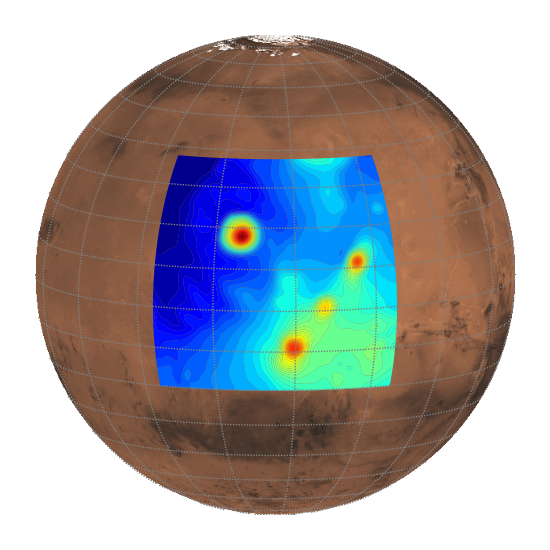
\includegraphics[width=0.8\textwidth]{domain_100.png} 
\end{center}
\mbox{}\\ 
\begin{center}
\huge{A. Spiga}\\
\email{aymeric.spiga}{upmc.fr}\\
Laboratoire de M\'et\'eorologie Dynamique\\
%Institut Pierre Simon Laplace\\
Universit\'e Pierre et Marie Curie, Paris, France\\
\mbox{}\\ 
\large \today \normalsize
\end{center} 
\end{titlepage} 


\clearemptydoublepage


%%%%%%%%%%%%%%%%%%%%%%
% TABLE DES MATIERES %
%%%%%%%%%%%%%%%%%%%%%%
\dominitoc
\ajusterletitrecourant{User Manual for the LMD Martian Mesoscale Model}
%\pagestyle{empty}
\tableofcontents
\clearemptydoublepage
%\pagestyle{fancy}


%%%%%%%%%%%%%%%%%%%%%%%%%%%%%%%%%%%%%%%%%%%%%%%%%%%%%%%%%%%%%%%
%%%%%%%%%%%%%%%%%%%%%%%%%%%%%%%%%%%%%%%%%%%%%%%%%%%%%%%%%%%%%%%
\mainmatter

%\clearemptydoublepage
%\chapter{Introduction}

\selectlanguage{english}
This document is a user manual for the Generic Climate Model
developed by the Laboratoire de M\'et\'eorologie
Dynamique of the CNRS in Paris.
It corresponds to the version of the model available since January 2011,
that includes the new dynamic code lmdz3.3
and input and output data in NetCDF format.
The physical part includes generalized correlated-k radiative transfer,
generalized tracer transport, and a water cycle that includes water vapour and ice transport,
radiative and thermodynamic effects, and simple hydrology.

Chapter~\ref{sc:apercu} of this document, to be read before any of the others,
describes the main features of the model.
The model is divided into two relatively independent parts:
(1) The hydrodynamic code, which integrates the fluid mechanical \emph{primitive equations} in time
over the globe, and (2) the physical parameterizations, which include the radiative transfer, tracer transport / evolution,
and surface-atmosphere interaction. It is followed by a list of references for anyone requiring a detailed
description of the physics and the numerical formulation of the parameterizations (Chapter~\ref{sc:phystd}).

For your {\bf first contact with the model}, Chapter~\ref{loc:contact1} guides the user through a practice simulation
(choosing the initial states and parameters and  visualizing the output files). The document then describes the code used for the model, including a user computer manual for compiling and running it (Chapter~\ref{sc:info}).

Chapter~\ref{sc:io} describes the input/output data of the model. The input files are the files needed to initialize the model (state of the atmosphere at instant $t0$ as well as a dataset of boundary conditions). The output files are ``historical files", archives of the atmospheric flow history as simulated by the model, the ``diagfi files", the ``stats files'', the daily averages, and so on. Common ways of editing or visualizing these files (editor ``ncdump" and the graphics software ``grads") are also explained.  Chapter~\ref{sc:water} explains how to run a simulation that includes the water cycle. Finally, Chapter~\ref{sc:rcm1d} will help you to use a 1-dimensional version of the model, which may be a simpler tool for some analysis work.
  
%
%\clearemptydoublepage
%\include{ch1}
%
\clearemptydoublepage
\ajusterletitrecourant{User Manual for the LMD Martian Mesoscale Model}
%\chapter*{
%Realistic modeling of the 
%Martian mesoscale and 
%microscale circulation :
%validation and first results.
%}
%\newpage





%\newpage
%\mbox{}
%\newpage

\chapter*{Foreword}

\vk
\paragraph{Welcome!} This manual describes how to use the Laboratoire de M\'et\'eorologie Dynamique (LMD) Martian Mesoscale Model. Many thanks for looking forward to using this model which development required countless hours of hard work! A significant part of the model development and validation have been funded by ESA and CNES which are acknowledged for their support.

\paragraph{Contact} The main contact to reach at LMD to become an user of the model is Aymeric SPIGA (main developper, \href{mailto:aymeric.spiga@upmc.fr}{\nolinkurl{aymeric.spiga@upmc.fr}}). Alternative contacts at LMD for mesoscale modeling inquiries are Ehouarn MILLOUR~\url{ehouarn.millour@lmd.jussieu.fr} or Fran\c cois FORGET~\url{francois.forget@lmd.jussieu.fr}. We are open to questions and suggestions on new scientific collaborations, teaching/outreach actions or contractual proposals.

\paragraph{Copyright (LMD)} The LMD Martian Mesoscale Model sources are made available on the condition that we make no representations or warranties regarding the reliability or validity of the model predictions nor the use to which such model predictions should be put, disclaim any and all responsibility for any errors or inaccuracies in the model predictions and bear no responsibility for any use made of this model predictions by any party. The scientific use of already published LMD Martian Mesoscale Model simulations is freely allowed provided that the reference paper \textit{Spiga and Forget} [2009]\nocite{Spig:09} is correctly quoted in all publications and that we are kept informed of usage and developments. If your study requires dedicated simulations with the LMD Martian Mesoscale Model, please consider including Aymeric SPIGA as a co-author of your work and asking, if needed, for help with writing the part related to mesoscale modeling. If your study requires additional work on a specific Martian physical parameterization, please consider including other members of the LMD team in addition to Aymeric SPIGA. The LMD Martian Mesoscale Model may not be put to any commercial use without specific authorization. 

\paragraph{Copyright (WRF)} Part of the LMD Martian Mesoscale Model is based on the terrestrial model WRF which is in the public domain. If you are an user of the LMD Martian Mesoscale Model, you are therefore an user of the WRF model. Please take a minute to fill in the WRF registration form so that the WRF development team knows about the people using their model: \url{http://www.mmm.ucar.edu/wrf/users/download/wrf-regist.php}. \noindent \scriptsize \emph{WRF was developed at the National Center for Atmospheric Research (NCAR) which is operated by the University Corporation for Atmospheric Research (UCAR). NCAR and UCAR make no proprietary claims, either statutory or otherwise, to this version and release of WRF and consider WRF to be in the public domain for use by any person or entity for any purpose without any fee or charge. UCAR requests that any WRF user include this notice on any partial or full copies of WRF. WRF is provided on an "AS IS" basis and any warranties, either express or implied, including but not limited to implied warranties of non-infringement, originality, merchantability and fitness for a particular purpose, are disclaimed. In no event shall UCAR be liable for any damages, whatsoever, whether direct, indirect, consequential or special, that arise out of or in connection with the access, use or performance of WRF, including infringement actions. WRF is a registered trademark of the University Corporation for Atmospheric Research (UCAR).} \normalsize

\clearemptydoublepage

\chapter{What is the LMD Martian Mesoscale Model?}\label{whatis}

\vk
This chapter comprises slightly edited excerpts from \textit{Spiga and Forget} [2009]\nocite{Spig:09}, dedicated to a general scientific and technical description of the LMD Martian Mesoscale Model, of its design and capabilities. Further details can be found in the reference \textit{Spiga and Forget} [2009]\nocite{Spig:09} paper and subsequent papers about mesoscale applications: e.g., \textit{Spiga and Lewis} [2010]\nocite{Spig:10dust} and \textit{Spiga et al.} [2011]\nocite{Spig:11ti}. Figure~\ref{modelstructure} summarizes the main points detailed in this introduction. This chapter is intended both for beginners and advanced users of the LMD Martian Mesoscale Model.

\begin{center}
\begin{figure}[p] 
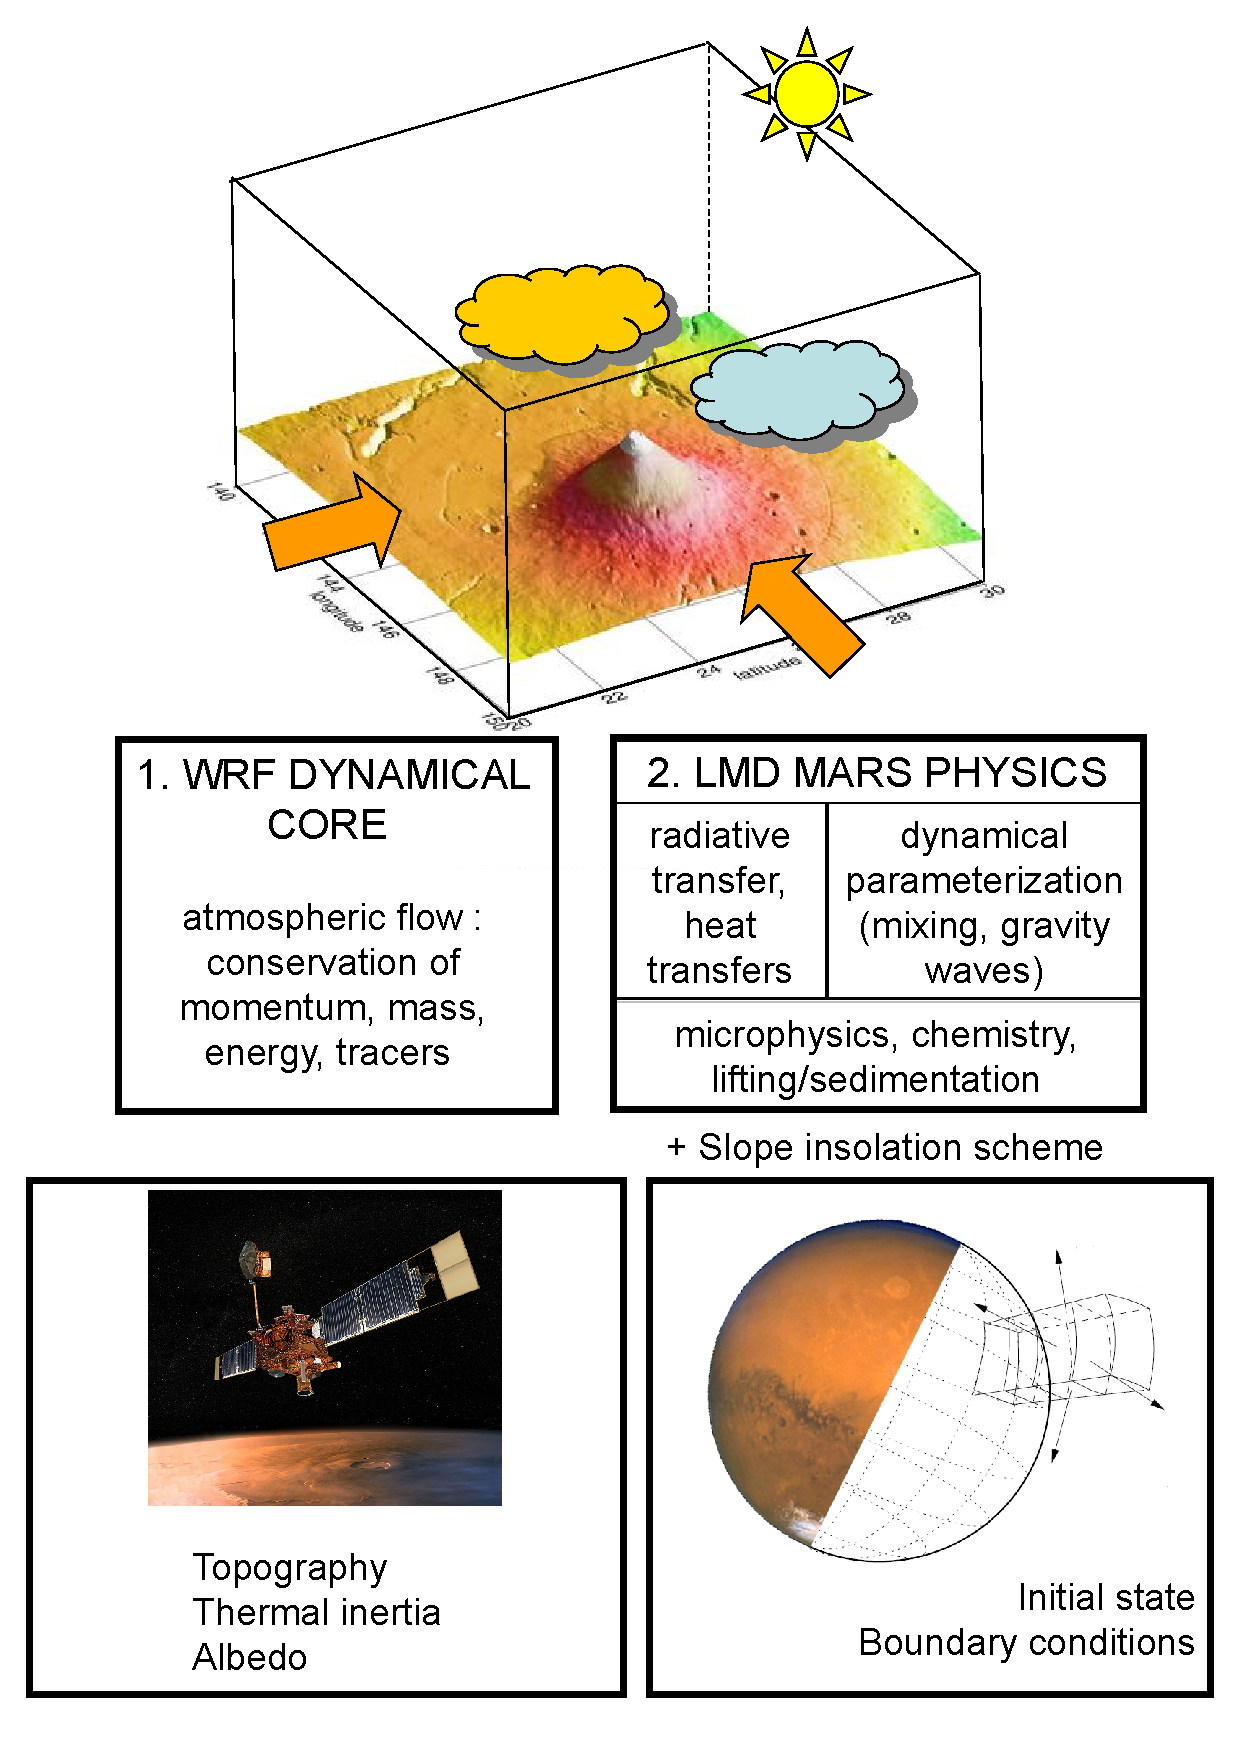
\includegraphics[width=0.99\textwidth]{meso.pdf} 
\caption{\label{modelstructure} An illustration of the LMD Martian Mesoscale Model design and capabilities.}
\end{figure}
\end{center}

\mk
\section{Dynamical core}

\sk
The numerical integration of the atmospheric fluid dynamic equations is performed in meteorological models by the dynamical core. The LMD Martian Mesoscale Model dynamical core is based on the stable and carefully tested, fully parallellized, Advanced Research Weather Research and Forecasting model (hereinafter referred as ARW-WRF) [\textit{Skamarock et al.}, 2005, 2008\nocite{Skam:08}\nocite{Skam:05}], developed for terrestrial applications at NCEP/NCAR (version 2.2.1 - November 2007).

\sk
The ARW-WRF mesoscale model integrates the fully compressible non-hydrostatic Navier-Stokes equations in a specific area of interest on the planet. Since the mesoscale models can be employed to resolve meteorological motions less than few kilometers, a scale at which the vertical wind acceleration might become comparable to the acceleration of gravity, hydrostatic balance cannot be assumed, as is usually done in General Circulation Models (GCMs).

\sk
Mass, momentum, entropy, and tracer conservation are ensured by an explicitly conservative flux-form formulation of the fundamental equations, based on mass-coupled meteorological variables (winds, potential temperature, tracers). Alternatively, these variables are recast into a reference profile plus a perturbation to reduce truncation errors [\textit{Skamarock et al.}, 2008]\nocite{Skam:08}. Tracer transport can be computed by an additional forward-in-time scheme based on the Piecewise Parabolic Method [\textit{Carpenter et al.}, 1990]\nocite{Carp:90}, with positive definite and monotonic properties
[\textit{Skamarock et al.}, 2006]\nocite{Skam:06}.

\sk
In the vertical dimension, the equations are projected, as suggested by \textit{Laprise} [1992]\nocite{Lapr:92}, on terrain-following mass-based coordinates (``eta levels"): $\eta = (\pi-\pi_t) / (\pi_s-\pi_t)$ where $\pi$ is the hydrostatic component of the pressure, $\pi_s$ the value at the surface and $\pi_t$ the (constant) upper boundary value. As shown in \textit{Laprise} [1992]\nocite{Lapr:92} and \textit{Janjic et al.} [2001]\nocite{Janj:01}, the choice of such vertical coordinates enables the integration of the ARW-WRF equations either in full non-hydrostatic mode or under the hydrostatic assumption. At the top of the domain, a free relaxation condition to zero vertical velocity is imposed (gravity wave absorbing layers can be defined as well).

\sk
In the horizontal dimension, the dynamical solver is available with three possible projections on the planetary sphere: Mercator (suitable for equatorial regions),  Lambert Conformal (for mid-latitudes),  and Polar Stereographic (for high-latitudes). Projections are defined by map scale factors, ensuring a regular computational grid whatever the map projection should be. Polar simulations are therefore devoid of any pole singularity, an usual drawback of the GCMs that requires the use of additional filtering. The spatial discretization is an Arakawa C-grid, where normal velocities are staggered one-half grid length from the thermodynamic variables [\textit{Arakawa}, 1966]\nocite{Arak:66}.

\sk
In the temporal dimension, a third-order Runge-Kutta integration scheme is employed for improved numerical accuracy and stability: the maximum stable Courant Friedrichs Lewy (CFL) numbers for advection are increased by a factor of two compared to the regular leapfrog integration scheme [\textit{Skamarock et al.}, 2008]. A time-splitting integration technique is implemented to prevent the meteorologically insignificant acoustic motions from triggering numerical instabilities [\textit{Klemp et al.}, 2007]\nocite{Klem:07}. Additional filters for acoustic external and internal modes damp residual instabilities possibly arising in the acoustic step integration.

\sk
In the ARW-WRF Runge-Kutta time-integration scheme, while pressure gradient and divergence terms are simply second order and centered, spatial discretizations of the advection terms for momentum, scalars and geopotential are 2nd through 6th order accurate [\textit{Wicker and Skamarock}, 2002]\nocite{Wick:02}. Martian simulations are performed with a 5th order discretized advection. One peculiarity of the odd-order advection discretization is the inherent inclusion of a dissipation term [\textit{Hundsdorfer et al.}, 1995]\nocite{Hund:95} with a coefficient proportional to the Courant number.

\sk
However, as was pointed out by \textit{Knievel et al.} [2007]\nocite{Knie:07}, this odd-ordered implicit scheme is not diffusive enough in low-wind or neutral/unstable stratification, and numerical noise in the wind fields might reach amplitudes comparable to the simulated winds. Such noise was found to be significant in the Martian case under near-surface afternoon superadiabatic conditions. The standard Martian simulations thus include the additional 6th order diffusion scheme developed by \textit{Knievel et al.}, with a removal parameter set for Martian applications to $20\%$ of the $2\,\Delta x$ noise in one timestep. While reducing the numerical noise near the surface to almost undiscernable amplitudes, the additional Knievel diffusion has little effect on the simulated meteorological fields.

\sk
Particular adaptations were required to use the ARW-WRF dynamical solver in the Martian environment. Physical constants, such as the acceleration of gravity and the planetary rotation rate, were converted to the Martian values. Vegetation and ocean-related variables were not used, and replaced with variables more suitable for the Martian applications (e.g., thermal inertia). Martian dates are given by the aerocentric solar longitude $L_s$, which indicates the position of Mars with respect to the Sun (0, 90, 180, 270 degrees are, respectively, the beginning of the northern hemisphere spring, summer, fall and winter). The terrestrial calendar was thus replaced with the LMD-GCM Martian calendar built on 669 Martian sols split in 12 ``aerocentric longitude"-based months (each of them is $L_s=30^{\circ}$ long, and thus encloses an irregular number of Martian sols due to the high eccentricity of the orbit), and one hour was defined as $1/24$ sol.

\mk
\section{Martian physics}

\sk
In any meteorological model, the 3D dynamical core is coupled with parameterization schemes (most often 1D) to compute at each grid point of the simulation domain the particular physics of the considered planetary environment: diabatic forcing of the atmospheric circulation (radiative transfer, soil thermal diffusion); sub-grid scale dynamical parameterizations (Planetary Boundary Layer [PBL] diffusion and mixing, convective adjustment); tracer sources and sinks (microphysical processes, chemistry, dust sedimentation and lifting). The LMD-MGCM complete physical parameterizations are interfaced with the adapted ARW-WRF dynamical core, described in the previous section, by a new ``driver" that is built on the same principles as the ARW-WRF terrestrial parameterization schemes, which are all switched off for the Martian applications. Thus, the LMD Martian Mesoscale Model shares the same comprehensive physical parameterizations as the LMD-MGCM, in order to simulate the Martian dust, CO$_2$, H$_2$O and photochemistry cycles [\textit{Forget et al.}, 1999; \textit{Montmessin et al.}, 2004; \textit{Lefevre et al.}, 2004].

\sk
\subsection{Physical parameterizations}

\sk
The radiative transfer in the model accounts for CO$_2$ gas infrared absorption/emission [\textit{Hourdin et al.}, 1992]\nocite{Hour:92} and visible and infrared dust absorption, emission and diffusion [\textit{Forget et al.}, 1998, 1999]\nocite{Forg:98grl}. Description of the CO$_2$ condensation processes in the model can be found in \textit{Forget et al.} [1998b]\nocite{Forg:98}. Thermal conduction in the soil is simulated by the 11-layer soil model developed by \textit{Hourdin et al.} [1993]\nocite{Hour:93} for Mars (soil density and soil specific heat capacity are set as constants). Turbulent closure is based on turbulent viscosity with coefficients calculated from the ``$2.5$-order" scheme by \textit{Mellor and Yamada} [1982]\nocite{Mell:82}, improved by \textit{Galperin et al.} [1988]\nocite{Galp:88}. In the case where vertical mixing is handled in the independent 1D physical packages, the native vertical mixing schemes in the ARW-WRF dynamical core are switched off, and the most appropriate choice for explicit horizontal diffusion is the built-in ARW-WRF scheme based on horizontal deformation [\textit{Smagorinsky}, 1963]\nocite{Smag:63}.

\sk
Recent improvements on the radiative transfer computations [\textit{Dufresne et al.}, 2005]\nocite{Dufr:05}, on the slope irradiance estimations [\textit{Spiga and Forget}, 2008]\nocite{Spig:08grl}, on the dust lifting and sedimentation [\textit{Forget et al.}, 1999b\nocite{Forg:99icm5}; \textit{Newmann et al.}, 2002]\nocite{Newm:02a}, on the water cycle and water ice clouds [\textit{Montmessin et al.}, 2004]\nocite{Mont:04}, and on the photochemical species [\textit{Lefevre et al.}, 2004]\nocite{Lefe:04}, particularly ozone [\textit{Lefevre et al.}, 2008]\nocite{Lefe:08}, are also natively included in the LMD Martian Mesoscale Model. The non-local thermodynamic equilibrium (NLTE) parameterizations for thermosphere applications [\textit{Gonz\'alez-Galindo et al.}, 2005\nocite{Gonz:05}] as well as estimations of the atmospheric exchanges with the Martian regolith [\textit{B\"ottger et al.}, 2005]\nocite{Bott:05}, are also available in the model.

%\sk
%Upcoming improvements of the LMD-MGCM physics [\textit{Forget et al.}, 2007]\nocite{Forg:07emsec}, following the recent measurements by instruments onboard Mars Express (MEx) and MRO, will be included in the LMD Martian Mesoscale Model too. Examples of future parameterizations that will be added in both models are the radiative effects of water ice clouds, which could significantly modify the atmospheric temperatures [\textit{Wilson et al.}, 2007]\nocite{Wils:07}, and the new dust radiative properties derived from recent measurements by the OMEGA instrument onboard MEx [\textit{M\"a\"att\"anen et al.}, 2008]\nocite{Maat:08} and the CRISM instrument onboard MRO [\textit{M.~J. Wolff and M. Vincendon}, personal communication, 2008].

\sk
Two physical parameterizations of the LMD-MGCM, specifically designed for synoptic-scale meteorological applications, are not used in the mesoscale applications.

\sk
Firstly, in the mesoscale domain, the topographical field is described with horizontal resolutions from tens of kilometers to hundreds of meters. The \textit{Lott and Miller} [1997]\nocite{Lott:97} subgrid-scale topographical drag parameterization and the \textit{Miller et al.} [1989]\nocite{Mill:89} gravity-wave drag scheme can thus be switched off, as the topographical influence on the atmospheric flow is computed by the dynamical core at the chosen mesoscale resolutions.

\sk
Secondly, in order to ensure numerical stability, and to account for subgrid-scale mixing processes insufficiently handled in the PBL scheme, it is usually necessary to modify any unstable layer with negative potential temperature gradients (an usual near-surface situation during Martian afternoons) into a neutral equivalent [\textit{Hourdin et al.}, 1993]. As pointed out by \textit{Rafkin} [2003b]\nocite{Rafk:03adj}, the use of such an artificial convective adjustment scheme might be questionable in Martian atmospheric models, should they be GCMs or mesoscale models. Since numerical stability is ensured in the LMD Martian Mesoscale Model by choosing the appropriate dynamical timestep with respect to the CFL condition, and using the aforementioned ARW-WRF nominal filters and diffusion schemes, the convective adjustment scheme used in the LMD-MGCM can thus be switched off in the LMD Martian Mesoscale Model. 

\mk
\subsection{Physical timestep}

\sk
Invoking physical packages often with respect to the dynamical computations was found to be necessary to accurately account for near-surface friction effects where the wind acceleration is particularly high, typically in regions of strong Martian topographically-driven circulation. In such areas, if the ratio between the physical timestep and the dynamical timestep is above $\sim 5$, the model predicts winds spuriously increasing with the chosen ratio and varying with the horizontal resolution. On the contrary, if this ratio is less than $\sim 5$, the simulated winds neither vary significantly with the chosen ratio nor with the horizontal resolution.

\sk
A ratio equal to 1 is chosen in the standard LMD Martian Mesoscale Model simulations. This choice is in conformity with the strategy adopted in the terrestrial ARW-WRF model. Besides, computing the physical parameterizations at the same frequency as the dynamical integration is profitable to some physical parameterizations, such as the formation of clouds (which is sensitive to rapid temperature change). Note that radiative transfer computations are usually carried out less often to save computational time.

\sk
When the ratio between the physical timestep and the dynamical timestep is superior to 1, two distinct strategies could be adopted. Interestingly, we found that splitting the physical tendency in equal parts and blending it with the dynamical tendency at each dynamical timestep computation is slightly more stable (understand: allows for higher dynamical timesteps) than applying the whole physical tendency when the physical parameterizations are computed, and letting the dynamical core naturally evolve until the next physics call. However, an analysis of the simulated meteorological fields in both cases does not reveal significant differences.

\mk
\section{Initial and boundary conditions}
\label{ssc:inibdy}

\mk
\subsection{Starting state and horizontal boundaries}

\sk
Mesoscale simulations can be performed in a limited domain anywhere on the planet. Thus, boundary conditions for the main meteorological fields (horizontal winds, temperature, tracers) have to be provided during the simulations, in addition to an atmospheric starting state. Idealized simulations usually require the use of periodic, symmetric or open boundary conditions, whereas real-case simulations need specified climatologies at the boundaries.

\sk
The specified boundary conditions and the atmospheric starting state are derived from previously performed $64\times48\times25$ (i.e., horizontal resolution of $5.625^{\circ}$ in longitude and $3.75^{\circ}$ in latitude, model top $\sim$~80~km~altitude) LMD-MGCM simulations which have reached equilibrium, typically after $\sim 10$ simulated years. GCM results are often used every Martian hour to constrain the mesoscale model at the domain boundaries. Temporal interpolations to each mesoscale timestep and spatial interpolations on the mesoscale domain are performed from the LMD-MGCM inputs. A relaxation zone of a given width (user-defined, usually 5 grid points) is implemented at the boundaries of the ARW-WRF domain to enable both the influence of the large-scale fields on the limited area, and the development of the specific mesoscale circulation inside the domain. The interpolations and the use of a relaxation zone prevent the prescribed meteorological fields at the lateral boundaries from having sharp gradients and from triggering spurious waves or numerical instabilities (the situation where the relaxation zone crosses steep topographical gradients should however be avoided).

\mk
\subsection{Nesting or single-domain strategy ?}
\label{ssc:nestingvalid}

\sk
The model includes one-way and two-way (or ``feedback") nesting capabilities. The nested simulations feature two kinds of domains where the meteorological fields are computed: the "parent" domain, with a large geographical extent, a coarse grid resolution, and specified boundary conditions, and the "nested" domains, centered in a particular zone of interest, with a finer grid resolution, and boundary conditions provided by its parent domain.

\sk
The nesting capabilities can be used only if deemed necessary, and single-domain simulations may be the primary type of run performed.

\sk
Firstly, employing the same physical parameterizations in the mesoscale model computations and in the GCM simulations defining the boundary and initial conditions, ensures a very consistent meteorological forcing at the boundaries of the mesoscale domain. This assumption was not denied by further examination of the performed simulations: mesoscale predictions are not unrealistically departing from the LMD-MGCM prescribed fields at the boundaries, and the mesoscale influence naturally adds to the synoptic (large-scale) tendency communicated at the boundaries. 

\sk
Secondly, the single-domain approach is appropriate as long as the variations of near-surface winds, pressure and temperature induced by ``passing" thermal tides through the east-west boundaries are not unrealistic. This criterion is specific to Martian mesoscale modeling and was described by \textit{Tyler et al.} [2002]. In the various simulations performed with the LMD Martian Mesoscale Model, a likely spurious influence of the passing thermal tides was only detected in the near-surface meteorological fields calculated at the $\sim 5$ near-boundaries grid points. The amplitudes of the departures were negligible ($\delta T \apprle 3$~K; $\delta u, \delta v \apprle 5\%$) and did not require the use of domains nested inside one semi-hemispheric parent domain [\textit{Tyler et al.}, 2002]. However, the analysis of the simulated fields at the near-boundaries grid points should be carried out with caution when choosing the single-domain approach. A practical solution to this drawback is to define a large domain, centered on the chosen area of interest, with a sufficient number of grid points ($75 \times 75$ being a minimal requirement).

\sk
Thirdly, \textit{Dimitrijevic and Laprise} [2005]\nocite{Dimi:05} showed, by the so-called ``Big Brother" approach, that the single-domain approach yields unbiased results when the boundary forcing involves a minimum of $\sim 8-10$ GCM grid points. Thus, given the resolution of the GCM fields used to constrain the LMD Martian Mesoscale Model, single-domain simulations with, for instance, a horizontal resolution of $20$~km shall be performed on at least $133 \times 88$ grid points. \textit{Antic et al.} [2006]\nocite{Anti:06} found that the ``$8-10$ grid points" limit can be lowered in situations of complex topography, because the dynamical influence of these mesoscale features is responsible for the larger part of the mesoscale circulation in the domain. Such situations are rather common on Mars, and the aforementioned ``minimal" grid can be of slightly smaller horizontal extent in areas such as Olympus Mons or Valles Marineris.

\sk
Thus the sizes of the simulation grids have to be chosen in order to ensure the applicability of the single-domain approach. The nesting technique is used only when defining a single domain with sufficient geographical extent would have required too many grid points to handle the computations within reasonable CPU time. For instance, with ``$64 \times 48$" GCM simulations as boundary conditions, the use of the single-domain strategy to model the Arsia Mons circulation at $5$ km resolution imposes a simulation grid of at least $531 \times 354$ points. The nesting technique is more suitable for this kind of simulation.

\mk
\subsection{Surface fields}

\sk
Surface static data intended for the mesoscale domain are extracted from maps derived from recent spacecraft measurements: 64 pixel-per-degree (ppd) MOLA topography [\textit{Smith et al.}, 2001]\nocite{Smit:01mola}, 8 ppd MGS/Thermal Emission Spectrometer (TES) albedo [\textit{Christensen et al.}, 2001]\nocite{Chri:01}, 20 ppd TES thermal inertia [\textit{Putzig and Mellon}, 2007]\nocite{Putz:07}. A smoother composite thermal inertia map derived from \textit{Palluconi and Kieffer} [1981]\nocite{Pall:81}, \textit{Mellon et al.} [2000]\nocite{Mell:00} and \textit{Vasavada et al.} [2000]\nocite{Vasa:00} can be alternatively used for better continuity with LMD-MGCM simulations. Except for CO$_2$ ice covered areas, emissivity is set to $0.95$. The roughness length $z_0$ is set to the constant value of $1$~cm, but further versions of the model will use spatially-varying $z_0$ [\textit{H\'ebrard et al.}, 2007]\nocite{Hebr:07}. Initial values for time-varying surface data, such as CO$_2$ and H$_2$O ice on the surface and soil temperatures, are derived from the GCM simulations. The latter initialization reduces the spin-up time for surface temperature to roughly one simulated sol.

\sk
The LMD Martian Mesoscale Model has the complete ability to simulate the dust cycle (lifting, sedimentation, transport). However, the high sensitivity of the results to the assumptions made on threshold wind stress and injection rate [\textit{Basu et al.}, 2004]\nocite{Basu:04} leads us to postpone these issues to future studies. Instead, similarly to the reference LMD-MGCM simulations, dust opacities are prescribed in the mesoscale model from 1999-2001 TES measurements, thought to be representative of Martian atmospheric conditions outside of planet-encircling dust storm events [\textit{Montabone et al.}, 2006]\nocite{Mont:06luca}. In the vertical dimension, as described in \textit{Forget et al.} [1999], and in accordance with the general consensus of well-mixed dust in equilibrium with sedimentation and mixing processes [\textit{Conrath}, 1975]\nocite{Conr:75}, dust mixing ratio is kept constant from the surface up to a given elevation $z_{\textrm{\tiny{max}}}$ above which it rapidly declines. Both in the nominal GCM and mesoscale simulations, $z_{\textrm{\tiny{max}}}$ as a function of areocentric longitude and latitude is calculated from the ``MGS scenario" [\textit{Forget et al.}, 2003]\nocite{Forg:03}.

\mk
\subsection{Vertical interpolation}

\sk
In the process of initialization and definition of boundary conditions, the vertical interpolation of GCM meteorological fields to the terrain-following mesoscale levels must be treated with caution. While deriving the near-surface meteorological fields from GCM inputs, one may address the problem of underlying topographical structures at fine mesoscale horizontal resolution, e.g., a deep crater that is not resolved in the coarse GCM case.

\sk
A crude extrapolation of the near-surface GCM fields to the mesoscale levels is usually acceptable for terrestrial applications. On Mars, owing to the low density and heat capacity of the Martian atmosphere, the surface temperature is to first order controlled by radiative equilibrium, and thus it is left relatively unaffected by variations of topography [e.g. \textit{Nayvelt et al.}, 1997]\nocite{Nayv:97}. A practical consequence, which renders an extrapolation strategy particularly wrong on Mars, is that the near-surface temperature and wind fields vary much more with the distance from the surface than with the absolute altitude above the areoid (or equivalently with the pressure level). Initial tests carried out with the extrapolation strategy showed that differences between temperatures at the boundaries and temperatures computed within the mesoscale domain close to these boundaries often reach $20-30$~K near the surface. An interpolation based only on terrain-following principles solves this problem near the surface but was found to lead to numerical instabilities at higher altitudes during the mesoscale integrations.

\sk
Therefore, input meteorological data need to be recast on intermediate pressure levels $P'$ with a low level smooth transition from terrain-following levels (for the near-surface environment) to constant pressure levels (for the free atmosphere at higher altitude). We thus have $P'(x,y)=\alpha + \beta \, P_s(x,y)$, $P_s$ being the surface pressure at the resolution of the GCM simulations. To ensure a realistic low-level transition, the technique described in \textit{Millour et al.} [2008]\nocite{Mill:08ddd}, based on high-resolution GCM results, is employed to calculate the $P'$ levels. The mesoscale surface pressure field $p_s$ is an input parameter of the method, since the near-surface adiabatic cooling over mountains and warming within craters are taken into account. Note that $p_s(x,y)$ is calculated from $P_s(x,y)$ on the basis of the high-resolution topography of the mesoscale domain $z(x,y)$ by $$p_s(x,y) = P_s(x,y) \, e^{ \frac{g \, [Z(x,y)-z(x,y)]}{R \, T(x,y)} }$$ \noindent where $Z(x,y)$ is the topography at the resolution of the GCM simulations, $R$ the gas law constant, $g$ the acceleration of gravity, and $T(x,y)$ the temperature predicted by the GCM $1$~km above the surface (see \textit{Spiga et al.} [2007]\nocite{Spig:07omeg}). Without reinterpolating the data, the intermediate pressure $P'$ levels are then simply converted into their mesoscale counterparts $p'$ by substituting $p_s$ for $P_s$ in the formula $P'(x,y)=\alpha + \beta \, P_s(x,y)$. Finally, the built-in ARW-WRF vertical interpolation onto the final mesoscale terrain-following levels can be performed, as the problem of extrapolation is solved by the use of the intermediate pressure levels $p'$.

\sk
The initial atmospheric state obtained through this ``hybrid" method ensures low-amplitude adjustments of the meteorological fields by the mesoscale model at the beginning of the performed simulations (i.e., in the first thousands of seconds). Furthermore, the continuity between the large-scale forcing and the mesoscale computations near the limits of the domain, as well as the numerical stability of the simulations, appear as significantly improved compared to methods either based on extrapolation (especially in areas of uneven terrains) or terrain-following interpolation.

%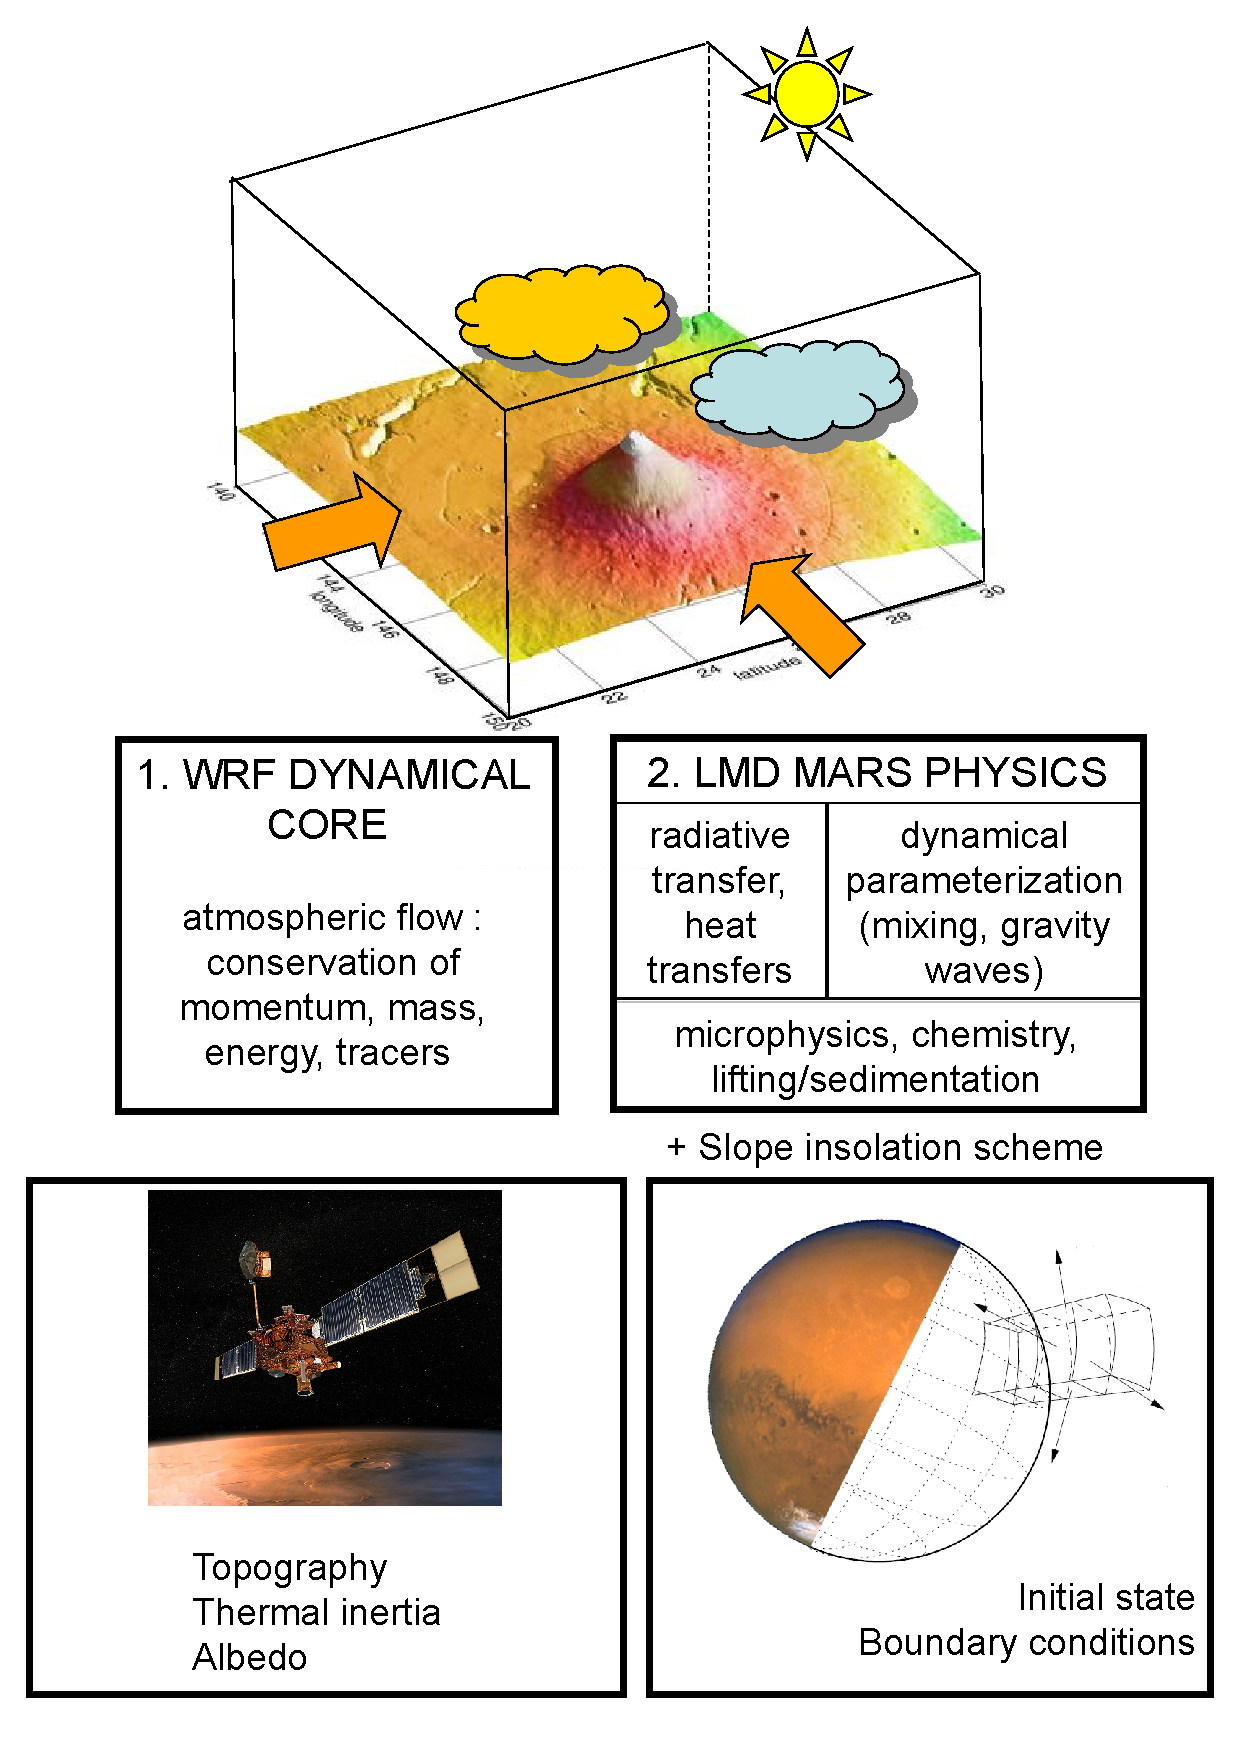
\includepdf[pages=1,offset=25mm -20mm]{meso.pdf}
\clearemptydoublepage


\chapter{Installing the model}\label{install}

\vk
This chapter is meant for first time users of the LMD Martian Mesoscale Model. We describe how to install the model on your system. Experience with either the terrestrial WRF mesoscale model or the LMD Martian GCM is not absolutely required, although it would help you getting more easily through the installation process.

\mk
\section{Prerequisites}

\sk
\subsection{General requirements}

\sk
In order to install the LMD Martian Mesoscale Model, please ensure the following prerequisites:
\begin{citemize}
\item your computer is connected to the internet;
\item you have~\ttt{200 Mo} free disk space available;
\item your OS is Linux\footnote{The model was also successfully compiled on MacOSX; ``howto" information is available upon request but could have become obsolete on recent versions of Apple hardware and software. It is probably possible to compile the model on Windows using Cygwin but this has not been implemented nor tested. This could work, but we recommend instead to install a Linux distribution on your computer (e.g. Ubuntu, Debian, Fedora, ...).} with a decent set of basic commmands (\ttt{sed}, \ttt{awk}, \ldots);
\item \ttt{bash}, \ttt{m4} and \ttt{perl} are installed on your computer;
\item at least one of the following Fortran compilers is installed on your computer
\begin{itemize}
\item Portland Group commercial compiler \ttt{pgf90}
\item G95 free compiler\footnote{Sources and binaries available on \url{http://www.g95.org}} \ttt{g95} 
\item Intel commercial compiler \ttt{ifort} 
\item GNU Fortran compiler \ttt{gfortran}
\end{itemize}
\item your C compiler is \ttt{gcc} and C development libraries are included;
\item \ttt{netCDF} libraries\footnote{The outputs from model computations are in netCDF format. This is a convenient self-describing file format widely used in atmospheric science and data analysis. Further information and downloads can be found in \url{http://www.unidata.ucar.edu/software/netcdf}.} have been compiled \emph{on your system with the Fortran compiler suite you aim to use to compile the model}. Three environment variables associated with the \ttt{NETCDF} libraries must be defined with the following commands\footnote{All command lines proposed in this document are defined in \ttt{bash} script language}:
\begin{verbatim}
declare -x NETCDF=/disk/user/netcdf  
declare -x NCDFLIB=$NETCDF/lib       
declare -x NCDFINC=$NETCDF/include       
\end{verbatim}
\end{citemize} 

\sk
\begin{finger}
\item If you want the environment variables to be persistent in your system, copy the \ttt{declare} command lines spread in this user manual in your \ttt{.bashrc} or \ttt{.bash\_profile}. 
\item You might also find useful -- though not mandatory -- to install on your system:
\begin{citemize}
\item \ttt{ncview}\footnote{ \url{http://meteora.ucsd.edu/~pierce/ncview\_home\_page.html} }: tool to visualize the contents of a netCDF file;
\item \ttt{nco}\footnote{ \url{ http://nco.sourceforge.net } }: tools to manipulate and modify netCDF files;
\item \ttt{epd}\footnote{ \url{ http://www.enthought.com/products/getepd.php }. A complete version is available free of charge for students and employees at degree-granting institutions. A limited version with essential librairies is available free of charge for any user (but e.g. cartography and \ttt{netCDF} python packages are not included in this free version). }: the python distribution suite packaged by Enthought, including many librairies for plotting, scientific computations, data analysis...
\end{citemize}
\end{finger}

\sk
\subsection{Compiling the terrestrial WRF model}\label{terrestrial}

\sk The LMD Martian Mesoscale Model is based on the terrestrial NCEP/NCAR ARW-WRF Mesoscale Model. As a first step towards the compilation of the Martian version, we advise you to check that the terrestrial model compiles on your computer with either \ttt{g95} or \ttt{pgf90} or \ttt{ifort}. On the ARW-WRF website \url{http://www.mmm.ucar.edu/wrf/users/download/get\_source.html}, you will be allowed to freely download the model after a quick registration process (click on ``New users"). Make sure to download the version 2.2 of the WRF model and copy the \ttt{WRFV2.2.TAR.gz} archive to your current working directory. Then please extract the model sources and configure the compilation process:
\begin{verbatim}
tar xzvf WRFV2.2.TAR.gz
cd WRFV2
./configure
\end{verbatim}

\sk
The \ttt{configure} script analyzes your architecture and proposes you several possible compilation options. Make sure to choose the ``single-threaded, no nesting" option related to either \ttt{g95} (should be option $13$ on a $32$~bits Linux PC) or \ttt{pgf90} (should be option $1$ on a $32$~bits Linux PC) or \ttt{ifort}. The next step is then to compile the WRF model by choosing the kind of simulations you would like to run. A simple and direct test consists in trying to compile the idealized case of a 2D flow impinging on a small hill:
\begin{verbatim}
./compile em_hill2d_x > log_compile 2> log_error &
\end{verbatim}
%
\begin{finger} \item In case you encounter problems compiling the ARW-WRF model, please read documentation on the website \url{http://www.mmm.ucar.edu/wrf/users}, contact the WRF helpdesk or search the web for your error message. Our team will not be able to offer support for the LMD Martian Mesoscale Model if the ARW-WRF model does not compile and run on your system. \end{finger}

\sk
If the compilation is successful, the file \ttt{log\_error} should be empty or only reporting few warnings. In the \ttt{main} folder two executables \ttt{ideal.exe} and \ttt{run.exe} should be found, which allows you to run\footnote{If you compiled the model with \ttt{g95}, \ttt{ideal.exe} will possibly complain about an error reading the namelist. Please move the line \ttt{non\_hydrostatic} below the line \ttt{v\_sca\_adv\_order} in the \ttt{namelist.input} file to solve the problem.} the test simulation:
\begin{verbatim}
cd test/em_hill2d_x
./ideal.exe
./wrf.exe
\end{verbatim}

\sk
During the simulation, the time taken by the computer to perform integrations at each dynamical timestep  is displayed in the standard output. The simulation should end with a message \ttt{SUCCESS COMPLETE WRF}. The model results are stored in a \ttt{wrfout} netCDF data file you might like to browse with a \ttt{NETCDF}-compliant software such as \ttt{ncview}, or read with your favorite graphical software. Once you have checked the WRF terrestrial model compiles and runs well on your system, you can delete all files related to the operations done in this section~\ref{terrestrial}.

\mk
\section{Main installation of the model sources}

\paragraph{Method 1: You were given a \ttt{LMD\_MM\_MARS.tar.gz} archive} Please set the environment variable \ttt{\$MESO} to point at the directory where you will install the model, and set the environment variable \ttt{\$MMM} as \ttt{\$MESO/LMD\_MM\_MARS}. Copy the \ttt{LMD\_MM\_MARS.tar.gz} file in the \ttt{\$MESO} directory and extract the files. Then execute the \ttt{prepare} script that would perform all installation tasks\footnote{Deflate the various compressed archives contained into \ttt{LMD\_MM\_MARS}, download the ARW-WRF sources from the web, apply a (significant) ``Martian patch" to these sources and build the structure of your \ttt{LMD\_MM\_MARS} directory}:
%
\begin{verbatim}       
declare -x MESO=/disk/user/MODELS
declare -x MMM=$MESO/LMD_MM_MARS
cp LMD_MM_MARS.tar.gz $MESO
cd $MESO
tar xzvf LMD_MM_MARS.tar.gz
cd $MESO/LMD_MM_MARS
ln -sf ./SRC/SCRIPTS/prepare .  ## not needed if script already in LMD_MM_MARS
./prepare  
\end{verbatim}

\begin{finger}
\item If you would like to use several versions of the model in separate folders, remember to change the \ttt{\$MESO} and \ttt{\$MMM} environment variables accordingly.
\end{finger}

\paragraph{Method 2: You were given a \ttt{svn} link \ttt{the\_link}} \emph{You must have Subversion (\ttt{svn}) installed on your system to follow this method}. Please use the name of our server repository combined to an \ttt{svn checkout} command to get the model sources\footnote{At this stage, it is essential to have registered to the WRF website (see foreword) because our server contains some part of the ARW-WRF sources.}. Please also set the environment variables \ttt{\$MESO} and \ttt{\$MMM} as is detailed below. The first download of the model sources could be a bit long. Compared to method~$1$, this method~$2$ using \ttt{svn} would allow you to easily get the latest updates and bug fixes done on the LMD Martian Mesoscale Model by the development team\footnote{If you are not interested by this feature, please replace the command line featuring \ttt{svn checkout} by the command line \ttt{svn export the\_link/LMDZ.MARS the\_link/MESOSCALE} }.

\begin{verbatim}
svn checkout the_link -N the_name_of_your_local_destination_folder
cd the_name_of_your_local_destination_folder
svn update MESOSCALE
[svn update LMDZ.MARS] ## only if you use the new physics (not recommended for a starter)
cd MESOSCALE
declare -x MESO=$PWD  ## put absolute link in your .bashrc
declare -x MMM=$MESO/LMD_MM_MARS
    ## to get latest updates later on
    cd the_name_of_your_local_destination_folder
    svn update
    svn log | more
\end{verbatim}

\mk
\section{Parallel computations (optional)}

\sk
Parallel computations with the Message Passing Interface (MPI) standard are supported by the LMD Martian Mesoscale Model. If you want to use this capability, you would have to add the installation of \ttt{MPICH2} or \ttt{openMPI} as a additional prerequisite. Once the installation is completed, it is required to define the environment variable \ttt{\$WHERE\_MPI} to point in your MPI \ttt{bin} directory, even if you added this directory to your \ttt{\$PATH} variable. 

%\begin{finger}
%\scriptsize
%\item An installation script for openMPI is available upon request (and information can be easily retrieved from the web).
%\item Here is a brief ``how-to" to install MPICH2, although this surely does not replace reading carefully installation notes and choosing which installation suits best your system. Please download the current stable version of the sources (e.g. we choose here an old version \ttt{mpich2-1.0.8.tar.gz} for the sake of illustration) on the MPICH2 website \url{http://www.mcs.anl.gov/research/projects/mpich2} and install the MPICH2 utilities by the following commands:
%\begin{verbatim}
%mkdir $your_software_dir/MPI ; mv mpich2-1.0.8.tar.gz $your_software_dir/MPI/ ; cd $your_software_dir/MPI
%tar xzvf mpich2-1.0.8.tar.gz ; cd mpich2-1.0.8
%./configure --prefix=$PWD --with-device=ch3:nemesis > conf.log 2> conferr.log &
%make > mk.log 2> mkerr.log &
%declare -x WHERE_MPI=$your_software_dir/MPI/mpich2-1.0.8/bin
%\end{verbatim}
%\normalsize
%\end{finger}

\clearemptydoublepage

\chapter{Compiling the model and running a test case}\label{compile}

\vk
This chapter is meant for first time users of the LMD Martian Mesoscale Model. We describe how to compile the program and run a test case. We start with important basics about how the model works and how it is organized.

\mk
\section{Basics}

\sk
\subsection{Necessary steps to run a simulation}\label{steps}

\sk
Any simulation that will be carried out with the LMD Martian Mesoscale Model comprises the five following steps. More details are given on these steps in the following chapters, but it is important at this stage to have this structure in mind. 

\sk 
\begin{itemize}
\item \textbf{Step 0} Compiling the model.
\item \textbf{Step 1} Running the LMD Global Circulation Model (GCM) to provide initial and boundary conditions for the mesoscale model.
\item \textbf{Step 2} Choosing the mesoscale limited-area domain of simulation. Running preprocessing programs to horizontally interpolate GCM meteorological fields and static data (topography, soil properties) to the chosen simulation domain.
\item \textbf{Step 3} Running preprocessing programs to vertically interpolate GCM meteorological fields and generate the initial and boundary conditions directly used by the mesoscale model.
\item \textbf{Step 4} Running the LMD Martian Mesoscale Model.
\end{itemize}

\sk
In this chapter, the general method to perform steps 0 and 4 is reviewed. Other steps are reviewed in chapter~\ref{zepreproc}; here the model is compiled and run for a test case with precomputed sample files for preprocessing steps 1, 2, 3. 

\sk
\subsection{Structure of the \ttt{LMD\_MM\_MARS} directory}

\sk
Please take the time to check the contents of the \ttt{LMD\_MM\_MARS} directories\footnote{If you used method~$2$, you will probably notice that other directories than~\ttt{LMD\_MM\_MARS} are present in \ttt{\$MESO}, but those are not important at this stage.} and sub-directories through the following command lines:
\begin{verbatim}
ls $MMM ; ls $MMM/*
\end{verbatim}

\sk
Contents of~\ttt{LMD\_MM\_MARS} directory:
\begin{citemize}
\item \ttt{makemeso}: this is the \ttt{bash} script to compile the model.
\item \ttt{SRC}: this is a directory containing the model sources.
\item \ttt{SIMU}: this is a directory containing scripts and files for an advanced use.
\item \ttt{WPS\_GEOG}: this is a directory containing static data used in step~2.
\end{citemize}

\sk
Contents of~\ttt{LMD\_MM\_MARS/SRC} subdirectory:
\begin{citemize}
\item \ttt{SCRIPTS}: this is a directory containing useful \ttt{bash} scripts for installation.
\item \ttt{WRFV2}: this is a directory containing main model sources (modified WRF dynamics + LMD physics in \ttt{mars\_lmd*}).
\item \ttt{PREP\_MARS}: this is a directory containing sources for the last part of step~1.
\item \ttt{WPS}: this is a directory containing sources for step~2.
\item \ttt{POSTPROC}: this is a directory containing postprocessing sources.
%\item \ttt{PYTHON}: this is a directory containing \ttt{python}-based graphical scripts.
\item \ttt{LES} and \ttt{LESnophys\_}: these are directories containing sources for Large-Eddy Simulations.
\end{citemize}

\sk
Contents of~\ttt{LMD\_MM\_MARS/SIMU} subdirectory:
\begin{citemize}
\item \ttt{callphys.def},\ttt{dustopacity.def}, \ttt{run.def}, \ttt{namelist.input\_full}, \ttt{namelist.input\_minim}, \ttt{namelist.input\_nests}, \ttt{namelist.input\_les}, \ttt{namelist.wps\_example}, \ttt{namelist.wps\_nests}, \ttt{namelist.wps.template}~: these are useful example and template files to guide you through setting up your own parameters for the LMD Martian Mesoscale Model simulations. 
\item \ttt{calendar}: this is a text file containing time management information in the model.
\item \ttt{runmeso}: this is a \ttt{bash} script that can be used once the model and preprocessing systems are installed; it prepares and runs a mesoscale simulation by going from step~1 to~4. 
\item \ttt{RUN}: this is a directory containing various files and scripts useful for advanced simulations.
\item \ttt{DEF}: this is a directory containing many examples of parameter files for simulations.
\end{citemize}

\sk
\begin{finger}
\item In pre-2011 versions of the model, the contents of the various directories listed here might differ. This has probably no impact on your use of the model if you ensure the following files and directories are present in \ttt{LMD\_MM\_MARS}:
\begin{citemize}
\item \ttt{makemeso}, \ttt{prepare}, \ttt{prepare\_ini}, \ttt{copy\_model}
\item \ttt{SRC/WRFV2}, \ttt{SRC/PREP\_MARS}, \ttt{SRC/WPS}
\item \ttt{SIMU/runmeso}, \ttt{SIMU/calendar}
\item \ttt{WPS\_GEOG}
\end{citemize}
\end{finger}

\mk
\section{Main compilation step}
\label{sc:makemeso}

\sk
\subsection{Description of the \ttt{makemeso} script}

\sk
The \ttt{bash} script which allows you to compile the LMD Martian Mesoscale Model is \ttt{makemeso}. It is an automated script which performs the following serie of tasks:
\begin{citemize}
\item ask the user about compilation settings;
\item retrieve some additional information about the system;
\item create a directory \ttt{\$MESO/LMD\_MM\_MARS/your\_compdir} which name depends\footnote{For example, a \ttt{your\_compdir} directory named \ttt{g95\_32\_single} is created if the user requested a \ttt{g95} compilation of the code for single-domain simulations on a 32 bits machine.} on the kind of compiler you are using, on whether your system is 32 or 64 bits, on whether sequential or parallel computations are planned and on the kind of simulations (idealized or real-case); 
\item generate with \ttt{copy\_model} a directory \ttt{your\_compdir/WRFV2} with links to \ttt{SRC/WRFV2} sources\footnote{A note to developers: this method ensures that any change to the model sources would be propagated to all the different \ttt{your\_compdir} installation folders.};
\item execute the WRF \ttt{configure} script with the correct options;
\item tweak the resulting \ttt{configure.wrf} file to include a link towards the Martian physics and various patches and specific compilation options;
\item calculate the total number of horizontal grid points handled by the LMD physics;
\item duplicate LMD physical sources if nesting is activated;
\pagebreak
\item compile the LMD physical packages with the appropriate \ttt{makegcm} command
and collect the compiled objects in the library \ttt{liblmd.a};
\begin{finger}
\item This step could be a bit long, especially if you are defining more than one domain. The \ttt{makemeso} script provides you with the full path towards the text file \ttt{log\_compile\_phys} in which you can check for compilation progress and possible errors. In the end of the process, you might find at the end of~\ttt{log\_compile\_phys} an error message associated to the generation of the final executable. Please do not pay attention to this, as the compilation of the LMD sources is meant to generate a library of compiled objects called \ttt{liblmd.a} instead of an executable.
\end{finger}
\item compile the modified Martian ARW-WRF solver and include the \ttt{liblmd.a} library; 
\begin{finger}
\item When it is the first time the model is compiled, this step could be quite long. The \ttt{makemeso} script provides you with a \ttt{log\_compile} text file where the progress of the compilation can be checked and a \ttt{log\_error} text file listing errors and warnings during compilation. A list of warnings related to \ttt{grib} utilities (not used in the Martian model) may appear and have no impact on the final executables.
\end{finger}
\item change the name of the executables in agreement with the
settings provided by the user.
\end{citemize}

\sk
\subsection{Use of the \ttt{makemeso} script}

\sk
To compile the model, change directory to \ttt{\$MMM} and execute the \ttt{makemeso} command:

\begin{verbatim}
cd $MMM
./makemeso
\end{verbatim}

\sk
You are asked a few questions by the \ttt{makemeso} script (see the list below) then it compiles the model for you. The script outputs a text file named \ttt{last} in which your answers to the questions are stored, which allows you to re-run the script without the ``questions to the user" step through the \ttt{makemeso < last} command line. 

\mk
\begin{asparaenum}[1.]%[\itshape Q1\upshape)]
\item \textbf{choice of compiler}\footnote{We advise you to compile the model on the same kind of system (computer + operating system + librairies) as the one you plan to use to run the model.} 
\item[1.bis] (mpi-based compilation) number of processors to be used
\item \textbf{number of grid points in longitude}\footnote{When you use parallel computations, please bear in mind that with $2$ (respectively $4$, $6$, $8$, $12$, $16$, $20$, $24$, $32$, $64$, $128$) processors the whole domain would be separated into $1$ (resp. $2$, $2$, $2$,  $3$,  $4$,  $4$,  $4$,  $4$,  $8$,   $8$) tiles over the longitude direction and $2$ (resp. $2$, $3$, $4$,  $4$,  $4$,  $5$,  $6$,  $8$,  $8$,  $16$) tiles over the latitude direction. Thus make sure that the number of grid points minus $1$ in each direction could be divided by the aforementioned number of tiles over the considered direction. For instance a~$82 \times 109$ horizontal grid is compliant with the use of~$12$ processors.} [61]
\item \textbf{number of grid points in latitude} [61]
\item \textbf{number of vertical levels} [61] 
\item \textbf{number of tracers}\footnote{The minimum number of tracers is 1 and not 0. Setting to 0 will actually make the script to set tracer number to 1.} [1]
\item \textbf{number of domains} [1]
%\item[6.bis] (not the first time you use \ttt{makemeso}) a question for advanced users [press any key]
%\item[6.ter] (new LMD physics) number of different scatterers to be used
\end{asparaenum}

\sk
The answers given in brackets above are the ones you want to use so that you will be able to run the test case proposed in the next section. Otherwise, before proceeding with \ttt{makemeso}, it is good to get used to gather the following information
\begin{itemize}
\item On which machine do you want to run the model? (a good practice is to compile on the same machine as the one used to run the model).
\item What is the horizontal resolution you want for your simulation? How many domains? How many tracers?
\item If parallel computations are employed: Do you have parallel librairies installed on the machine you chose? How much processors you want to use? 
\end{itemize}

\mk
A key question that often arises when using the LMD Martian Mesoscale Model is: when does the model has to be recompiled? The set of questions asked by~\ttt{makemeso} give some hints about this. Suppose you compiled a version of the model for a given set of parameters $1$ to $6$ to run a specific compilation. If you would like to run another simulation with at least one of parameters $1$ to $6$ subject to change, the model needs to be recompiled\footnote{This necessary recompilation each time the number of grid points, tracers and domains is modified is imposed by the LMD physics code. The WRF dynamical core alone is more flexible.} with \ttt{makemeso} (cf. also chapter~\ref{zeparam}).

\mk
Note that the \ttt{makemeso -h} command lists the various options that can be used in the \ttt{makemeso} script. Most options should be used only by advanced users and some of them will be described in the following chapters. At this stage, the only option of \ttt{makemeso} which can be useful to you is \ttt{-f} which forces the model to be recompiled from scratch (this is for instance very useful if a previous compilation ran into problems, or was interrupted by the user). If you already compiled the model succesfully, but the model fails to compile a few days later for reasons unrelated to your operations on your system or on the model file, we recommend you to use the \ttt{-f} option in \ttt{makemeso} to try to recompile the model\footnote{A more extreme solution if \ttt{makemeso -f} does not solve your problem is to remove the corresponding \ttt{your\_compdir} directory. See chapter~\ref{faq}}.

\scriptsize
\codesource{makemesohelp}
\normalsize

\mk
\section{Running a simple test case}
\label{sc:arsia}

\sk
We assume here that you had successfully compiled the model with \ttt{makemeso} at the end of the previous section and you had based your answers to the \ttt{makemeso} script on the indications in brackets. You should then find in the \ttt{your\_compdir} directory the \ttt{real\_x61\_y61\_z61\_d1\_t1\_p1.exe} and~\ttt{wrf\_x61\_y61\_z61\_d1\_t1\_p1.exe} executables.

\sk
In order to test the compiled executables, a ready-to-use test case (with pre-generated initial and boundary conditions) is proposed in the \ttt{LMD\_MM\_MARS/SIMU/DEF/TESTCASE} folder (use the \ttt{EXEC\_TO\_GET\_data.sh} command to get the initial and boundary condition files). This test case simulates the hydrostatic atmospheric flow around Arsia Mons (Figure~\ref{arsia}) during half a sol in springtime with constant thermal inertia, albedo and dust opacity\footnote{Though the simulation reproduces some reasonable features of the mesoscale circulation around Arsia Mons (e.g. slope winds), it should not be used for scientific purpose, for the number of grid points is unsufficient for single-domain simulation and the integration time is below the necessary spin-up time.}.

\sk
To launch the test simulation, please type the following commands, replacing if needed the \ttt{LATEST} directory with its corresponding value on your system. In the end, the model should run and output the computed meteorological fields in netCDF files named \ttt{wrfout*}. Feel free to browse those files with \ttt{ncview} or your favorite graphical tool to check if the simulated fields look reasonable. 
%
\begin{verbatim}
cd $MMM/SIMU/DEF/TESTCASE
./EXEC_TO_GET_data.sh (only once)
ln -sf ../../../LATEST/wrf_x61_y61_z61_d1_t1_p1.exe wrf.exe  
nohup wrf.exe > log_wrf &
\end{verbatim}

\sk
The files contained in \ttt{TESTCASE} prior to launching the simulations with the \ttt{wrf.exe} command illustrate which files are needed to perform step 4, i.e. running a LMD Martian Mesoscale Model simulation\footnote{For the test case presented here, a file named \ttt{dustopacity.def} is needed because for the sake of simplicity of this test case, we set idealized uniform dust opacity. The file \ttt{namelist.wps} is included in the \ttt{TESTCASE} folder for further reference but not needed at this stage.}. 
\begin{itemize}
\item \ttt{namelist.input}: text file containing parameters for the dynamical core
\item \ttt{callphys.def}: text file containing parameters for the physics parameterizations
\item \ttt{wrf.exe}: the model executable (or a link to it) as compiled by \ttt{makemeso}
\item \ttt{wrfinput\_d01} and \ttt{wrfbdy\_d01}: data files containing initial and boundary conditions
\end{itemize}

\begin{center} 
\begin{figure}[h!]
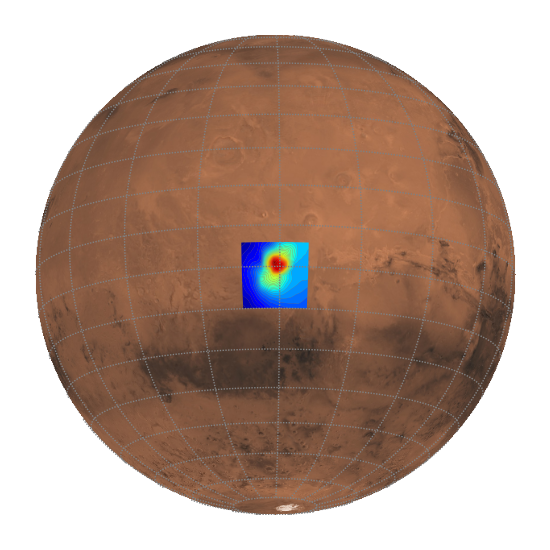
\includegraphics[width=0.5\textwidth]{arsiadomain.png} 
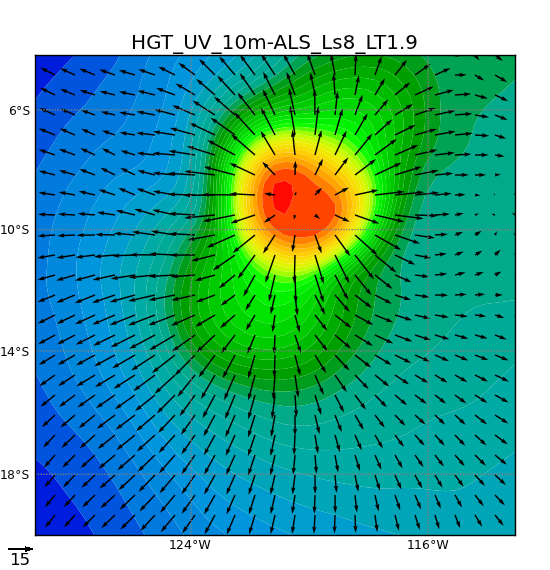
\includegraphics[width=0.5\textwidth]{LMD_MMM_d1_20km_HGT_UV_10m-ALS_Ls8_LT1_100.png}
\caption{\label{arsia} [Left plot] Simulation domain defined in the test case proposed as a demonstrator for running the LMD Martian Mesoscale Model. [Right plot] Nighttime winds predicted by the model~$10$~m above the surface. Both plots have been generated by command-line scripts written in~\ttt{python + numpy + matplotlib} (see chapter~\ref{postproc}).}
\end{figure}
\end{center}

\bk
%\scriptsize
\begin{finger}
\item If you compiled the model using MPI, the command to launch a simulation is slightly different:
%
\begin{verbatim}
[if several connected machines, create a file mpd.hosts with machine names...]
[... and make sure that ssh between machines does not need authentification]
mpirun [-f mpd.hosts] -np number_of_processors wrf.exe < /dev/null &      
tail -20 rsl.out.000? # to check the outputs
\end{verbatim}
%%echo barry.lmd.jussieu.fr > ~/mpd.hosts
%%echo white.lmd.jussieu.fr >> ~/mpd.hosts
%%echo loves.lmd.jussieu.fr >> ~/mpd.hosts
%%echo tapas.lmd.jussieu.fr >> ~/mpd.hosts	
%%mpdboot  -n 4
%%mpdtrace
%%mpirun -l -np 16 wrf.exe < /dev/null &   # NB: mpirun is only a link to mpiexec
\end{finger}
%\normalsize

\clearemptydoublepage

\chapter{Setting simulation parameters}\label{zeparam}

\vk
Here we describe how to set the parameters defining a simulation with the LMD Martian Mesoscale Model. As it was detailed in~\ref{sc:arsia}, two main parameter files are needed to run the model. Many examples of such files for martian mesoscale simulations can be found in \ttt{\$MMM/SIMU/DEF}:
\begin{enumerate}
\item The parameters related to the dynamical part of the model (dynamical core) can be set in the file \ttt{namelist.input} according to the ARW-WRF namelist formatting.
\item The parameters related to the physical part of the model (physical parameterizations) can be set in the file \ttt{callphys.def} according to the LMD-GCM formatting.
\end{enumerate}

\mk
\section{Dynamical settings}

\sk
\subsection{Description of \ttt{namelist.input}}

\sk
The file \ttt{namelist.input} controls the behavior of the dynamical core in the LMD Martian Mesoscale Model. This file is organized as a Fortran namelist with explicitely named categories:
\begin{citemize}
\item \ttt{time\_control}: set simulation start/end time and frequency of outputs;
\item \ttt{domains}: set the extent and grid spacing of the simulation domain(s) in the horizontal and vertical dimension, as well as the timestep for numerical integration;
\item \ttt{physics}: set parameters related to the dynamics / physics interface;
\item \ttt{dynamics}: set parameters controlling dynamical integrations (accuracy, diffusion, filters);
\item \ttt{bdy\_control}: set parameters related to boundary conditions and relaxation rows between model integrations and boundary conditions;
\item \ttt{grib2}, \ttt{fdda}, \ttt{namelist\_quilt}: not relevant for Mars, only present for continuity.
\end{citemize}

\sk %answer \ttt{y} to the last question.
Many parameters in the \ttt{namelist.input} file are optional in the Martian version\footnote{E.g., in the \ttt{namelist.input} file associated to the Arsia Mons test case presented in the previous chapter, the parameter \ttt{non\_hydrostatic} is set to false to assume hydrostatic equilibrium, whereas standard simulations are non-hydrostatic. Compared to the file the ARW-WRF users are familiar with (see generic description in \ttt{\$MMM/SRC/WRFV2/run/README.namelist}), typical \ttt{namelist.input} files for LMD Martian Mesoscale Model simulations are much shorter.} and their default values are defined in the file \ttt{\$MMM/SRC/WRFV2/Registry/Registry.EM}\footnote{Changing default values in \ttt{\$MMM/SRC/WRFV2/Registry/Registry.EM} should be avoided even if you are an advanced user.}. The only mandatory parameters in \ttt{namelist.input} are within the~\ttt{time\_control} and~\ttt{domains} categories. The minimal version of the \ttt{namelist.input} file corresponds to standard simulations with the model\footnote{You may find the corresponding file in \ttt{\$MMM/SIMU/namelist.input\_minim}.}:
%
\scriptsize
\codesource{namelist.input_minim}
\normalsize

\sk
A more detailed description of the \ttt{namelist.input} file is given in what follows\footnote{You may find the corresponding file in \ttt{\$MMM/SIMU/namelist.input\_full}.}, with all available (mandatory or optional) parameters to be set by the user. Each parameter is commented to understand its impact on the mesoscale simulations. Optional parameters are given with their default values. We have adopted labels to describe the specifics of each parameter with respect to the $5$~steps detailed in section~\ref{steps} (compilation, preprocessing, run):

\sk
\begin{citemize}
\item \ttt{(r)} indicates parameters which modifications imply a new compilation\footnote{A full recompilation using the option \ttt{makemeso -f} is not needed here.} of the model using \ttt{makemeso} (step 0);
\item \ttt{(p1)}, \ttt{(p2)}, \ttt{(p3)} mention parameters which modification implies a new processing of initial and boundary conditions (see chapter~\ref{zepreproc}), corresponding respectively to step~1, 2, 3; \ttt{(p1)} means the user has to carry out again steps~1 to 3 before being able to run the model at step~4; \ttt{(p2)} means the user has to carry out again steps~2 to~3 before model run at step~4; 
\item no label means that once you have modified the parameter, you can simply start directly at step~4 (running the model);
\item \ttt{(*d)} denotes dynamical parameters which modification implies non-standard simulations -- please read \ttt{\$MMM/SRC/WRFV2/run/README.namelist} and use with caution, i.e. if you know what you are doing; after modifying those parameters you can simply start at step~4.
\item \ttt{(*)} denotes parameters not to be modified;
\item \ttt{(n)} describes parameters involved when nested domains are defined (see chapter~\ref{nests}).
\end{citemize}

\sk
\small
\codesource{namelist.input_full}
\normalsize

\sk
\subsection{Important advice on filling \ttt{namelist.input}}\label{namelist}

\paragraph{Test case} An interesting exercise is to analyze comparatively the \ttt{TESTCASE/namelist.input} file (cf. section~\ref{sc:arsia}) with the reference \ttt{namelist.input\_full} given above, so that you could understand which settings are being made in the Arsia Mons test simulation. Then you could try to modify parameters in the \ttt{namelist.input} file and re-run the model to start getting familiar with the various settings. Given that the test case relies on pre-computed initial and boundary conditions, not all parameters can be changed in the \ttt{namelist.input} file at this stage.

\paragraph{Syntax} Please pay attention to rigorous syntax while editing your personal \ttt{namelist.input} file to avoid reading error. If the model complains about this at runtime, start again with the available template \ttt{\$MMM/SIMU/namelist.input\_full}.

\paragraph{Time management} Usually the user would like to start/end the mesoscale simulation at a given solar aerocentric longitude~$L_s$ or a given sol in the Martian year\footnote{Information on Martian calendars: \url{http://www-mars.lmd.jussieu.fr/mars/time/solar_longitude.html}.}. In the \ttt{namelist.input} file, start/end time is set in the form year / month / day with each month corresponding to a ``slice" of~$30^{\circ}$~$L_s$. The file~\ttt{\$MMM/SIMU/calendar} (reproduced in appendix) is intended to help the user to perform the conversion prior to filling the \ttt{namelist.input} file. In the above example of \ttt{namelist.input\_minim}, the simulation with the LMD Martian Mesoscale Model takes place on month~7 and day~1, which corresponds to~$L_s \sim 180^{\circ}$ according to the \ttt{calendar} file. In the Arsia Mons test case, the simulation with the LMD Martian Mesoscale Model takes place on month~1 and day~17, which corresponds to~$L_s \sim 8^{\circ}$.

\mk
\section{Physical settings}

\mk
The file \ttt{callphys.def} controls the behavior of the physical parameterizations in the LMD Martian Mesoscale Model. Modifying \ttt{callphys.def} implies to recompile the model only if the number of tracers has changed. This file is organized very similarly to the corresponding file in the LMD Martian GCM, which user manual can be found at \url{http://web.lmd.jussieu.fr/~forget/datagcm/user_manual.pdf}. Here are the \ttt{callphys.def} contents with typical mesoscale settings:

\vskip -0.5cm
\codesource{callphys.def}

\mk
\begin{finger}
\item In the provided example, convective adjustment \ttt{calladj}, gravity wave parameterization \ttt{calllott} and non-local thermodynamic equilibrium schemes \ttt{callnlte} are turned off, as is usually the case in typical Martian tropospheric mesoscale simulations (see chapter~\ref{whatis}).
\item \ttt{iradia} sets the frequency (in dynamical timesteps) at which the radiative computations are performed. To obtain the interval in seconds at which radiative computations are performed, one simply has to multiply \ttt{iradia} to the value of \ttt{time\_step} in \ttt{namelist.input}.
\item \ttt{iaervar=4} and~\ttt{iddist=3} defines the standard ``Mars Global Surveyor" dust scenario (see chapter~\ref{whatis}). It is the recommended choice.
\end{finger}

\clearemptydoublepage

\chapter{Preprocessing utilities}\label{zepreproc}

\vk
In this chapter, we describe the installation and use of the preprocessing tools to define the domain of simulation, calculate an initial atmospheric state and prepare the boundary conditions for the chosen simulation season and time of day. This corresponds to steps 1,2,3 as defined in section~\ref{steps}. These operations would eventually allow you to run your own simulations at the specific season and region you are interested in, with a complete ability to modify any of the parameters in \ttt{namelist.input}, including the ones labelled with~\ttt{(p1)}, \ttt{(p2)} or \ttt{(p3)}.

\mk
\section{Installing the preprocessing utilities}

\sk
The compilation operations indicated here need to be done only once on a given system with a given compiler. 

\sk
\subsection{Prerequisites}

\sk
First and foremost, since the preprocessing utilities could involve files of quite significant sizes, it is necessary to define a directory where these files would be stored. Such a directory (e.g. \ttt{/bigdisk/user}) must be linked with the name \ttt{TMPDIR} as follows. In addition, three directories \ttt{GCMINI}, \ttt{WPSFEED}, \ttt{WRFFEED} have to be created in \ttt{\$MESO/TMPDIR} as indicated below.

\begin{verbatim}
ln -sf /bigdisk/user $MESO/TMPDIR
mkdir $MESO/TMPDIR/GCMINI
mkdir $MESO/TMPDIR/WPSFEED
mkdir $MESO/TMPDIR/WRFFEED
\end{verbatim}

\sk
A second prerequisite to the installation of the preprocessing tools is that the LMD Martian Mesoscale Model was compiled at least once. If this is not the case, please compile the model with the \ttt{makemeso} command described in section~\ref{sc:makemeso}. The compilation process created an installation directory adapted to your particular choice of compiler$+$machine (what we named \ttt{your\_compdir} in section~\ref{sc:makemeso}, which could be for instance \ttt{g95\_32\_single}). The preprocessing tools will also be installed in this directory. Please type the following commands:

\begin{verbatim}
cd $MMM/your_compdir
ln -sf ../SRC/SCRIPTS/prepare_ini .
./prepare_ini
\end{verbatim}
%%echo $PWD

\sk
\subsection{Compiling preprocessing utilities}

\sk
The script \ttt{prepare\_ini} plays for the preprocessing tools a similar role as the script \ttt{copy\_model} for the model sources: files are simply linked to their actual location in the \ttt{SRC} folder. Once you have executed \ttt{prepare\_ini}, please check that two folders were generated: \ttt{PREP\_MARS} and \ttt{WPS}. In the \ttt{PREP\_MARS} directory, please compile the programs \ttt{create\_readmeteo.exe} and \ttt{readmeteo.exe}, using the compiler mentioned in the name of the current installation directory. In the \ttt{WPS} directory, please compile the programs \ttt{geogrid.exe} and \ttt{metgrid.exe}. Here are the useful commands:

\begin{verbatim}
cd your_compdir/PREP_MARS/
./compile_pgf [or] ./compile_g95 [or] ./compile_ifort  
ls -lt create_readmeteo.exe readmeteo.exe
cd ..
cd WPS/
clean
./configure     ## select your compiler + 'NO GRIB2' option
./compile
ls -lt geogrid.exe metgrid.exe
\end{verbatim}

\sk
Apart from the executables just compiled, the preprocessing utilities include \ttt{real.exe}, which was compiled by the \ttt{makemeso} script along with the mesoscale model executable \ttt{wrf.exe}\footnote{Even though the name of the executable reads e.g. \ttt{real\_x61\_y61\_z61\_d1\_t1\_p1.exe}, such program is not related to the specific \ttt{makemeso} parameters -- contrary to the \ttt{wrf.exe} executable. We just found that renaming the (possibly similar if the model sources were not modified) \ttt{real.exe} executable was a practical way not to confuse between executables compiled at different moments.} (cf. chapter~\ref{compile}). \ttt{real.exe} should be copied or linked in the simulation directory (e.g. \ttt{TESTCASE} for the Arsia Mons test case) to be at the same level than \ttt{namelist.input}.

\begin{verbatim}
cp your_compdir/real_*.exe your_simulation_directory/
cp your_compdir/wrf_*.exe your_simulation_directory/
\end{verbatim}

\sk
\subsection{Preparing input static data}\label{wpsgeog}

\sk
All the static data (topography, thermal inertia, albedo) needed to initialize the model are included in the \ttt{\$MMM/WPS\_GEOG} directory. By default, only coarse-resolution datasets\footnote{These coarse-resolution datasets correspond to the fields stored in the file \ttt{surface.nc} known by LMD-MGCM users: \url{http://web.lmd.jussieu.fr/~forget/datagcm/datafile/surface.nc} } are available, but the directory also contains sources and scripts to install finer resolution datasets: 32 and/or 64 pixel-per-degree (ppd) MOLA topography (\ttt{mola\_topo32} and \ttt{mola\_topo64}), 8 ppd MGS/Thermal Emission Spectrometer (TES) albedo (\ttt{albedo\_TES}), 20 ppd TES thermal inertia (\ttt{thermal\_TES}). The role of the \ttt{build\_static} script is to automatically download these datasets from the web (namely PDS archives) and convert them to an acceptable format for a future use by the preprocessing utilities:

\begin{verbatim}
cd $MMM
ln -sf SRC/SCRIPTS/build_static .
./build_static
\end{verbatim}

\sk
\begin{finger}
\item Please install the \ttt{octave} free software\footnote{Available at \url{http://www.gnu.org/software/octave} } on your system to execute the \ttt{build\_static} script\footnote{ Another solution is to browse into each of the directories within \ttt{WPS\_GEOG/res}, download the data with the shell scripts and execute the \ttt{.m} scripts with either \ttt{octave} or the commercial software \ttt{matlab} (just replace \ttt{\#} by \ttt{\%}). }. 
\item Building the MOLA 64ppd database can be quite long; hence this is not performed by default by the \ttt{build\_static} script. If you would like to build this database, please remove the \ttt{exit} command in the script, just above the commands related to the MOLA 64ppd.
\item If you do not manage to execute the \ttt{build\_static} script, ready-to-use datafiles can be found in the link \url{ftp://ftp.lmd.jussieu.fr/pub/aslmd} and must be extracted in \ttt{\$MMM/WPS\_GEOG}.
\item The resulting \ttt{WPS\_GEOG} directory can reach a size of several hundreds of Mo. You might move such a folder in a place with more disk space available and define a link~\ttt{WPS\_GEOG} in \ttt{\$MMM}.
\end{finger}

\sk
\subsection{Compiling the GCM for initial and boundary conditions}

\sk
The LMD Martian GCM needs to be run to compute meteorological fields that will be used as initial and boundary conditions each one or two Martian hours by the limited-area LMD Martian Mesoscale Model. Hence the LMD Martian GCM must be compiled in your system (see the LMD-MGCM user manual for further details \url{http://web.lmd.jussieu.fr/~forget/datagcm/user_manual.pdf}). If you did not get the model using the \ttt{svn} method, please request us to send you an archive containing the LMD-MGCM named \ttt{LMDZ.MARS.meso.tar.gz}, to be extracted in the \ttt{\$MESO} directory. If you got the model using \ttt{svn}, you do not have to request this file. In the \ttt{\$MESO/LMDZ.MARS} directory, a script named \ttt{compile} can be found and must be used \emph{on the system you plan to run the mesoscale model on} to compile the GCM. The \ttt{compile} script is actually just a wrapper for the \ttt{makegcm} script which compile the GCM for you; the default \ttt{makegcm} script only works with Portland Group Fortran compiler \ttt{pgf90} but scripts to compile the model using other Fortran compilers (including \ttt{g95} or \ttt{ifort}) are also available. The following commands should yield the compilation of two executables \ttt{newstart.e} and \ttt{gcm.e}:

\begin{verbatim}
cd $MESO/LMDZ.MARS
[edit $MESO/LMDZ.MARS/libf/phymars/datafile.h & fill absolute link $MMM/WPS_GEOG]
[edit compile if needed]
./compile
\end{verbatim}

\sk
The other necessary operation to prepare the LMD-MGCM for step~1 is to store a set of initial states for the LMD-MGCM to start with, based on previous typical LMD-MGCM runs having reached equilibrium after ten years of integration. A reference database\footnote{If another database is used, \ttt{compile} must be edited; default is~$64 \times 48 \times 32$ GCM runs with~$2$ tracers.} can be found in the following online archive~\url{ftp://ftp.lmd.jussieu.fr/pub/aslmd/STARTBASE_64_48_32_t2.tar.gz}. This archive must be extracted somewhere on a disk that would be accessible to the system you plan to run the mesoscale model on. A link named~\ttt{startbase} towards the \ttt{STARTBASE\_64\_48\_32\_t2} directory must be created in the directory~\ttt{\$MESO/LMDZ.MARS/myGCM}. 

\begin{verbatim}
ln -sf where_is_your_startbase/STARTBASE_64_48_32_t2 startbase
\end{verbatim}

\sk
It is important to check that the chosen reference database 1. spans the season desired for the mesoscale simulation; 2. includes the right number of tracers and vertical extent; and 3. uses GCM parameterizations that are close to the ones employed in the subsequent mesoscale simulations.

\sk
GCM integrations can then be launched in~\ttt{\$MESO/LMDZ.MARS/myGCM} using~\ttt{launch\_gcm}.

\mk
\section{Running the preprocessing utilities}

\sk
\subsection{General overview}\label{changeparam}

\sk
When you run a simulation with \ttt{wrf.exe} (e.g. section \ref{sc:arsia}), the program attempts to read the initial state in \ttt{wrfinput\_d01} and the domain boundary conditions in \ttt{wrfbdy\_d01}. The whole chain of data conversion and interpolation needed to generate those files is summarized in the diagram on Figure~\ref{preproc}. Three distinct preprocessing steps are necessary to generate the final files (steps are numbered 1,2,3 as in section~\ref{steps}). Figure~\ref{preproc} helps to better understand the labels \ttt{(p1)}, \ttt{(p2)}, \ttt{(p3)} used to describe \ttt{namelist.input} parameters in chapter~\ref{zeparam}. For instance: 
\begin{finger}
\item changing the season of simulation implies to re-run the LMD Mars GCM for this specific season to prepare initial and boundary conditions for the mesoscale model. Hence e.g. \ttt{start\_month} is labelled with \ttt{(p1)} because changing this in \ttt{namelist.input} requires a complete reprocessing from step~$1$ to step~$3$ to successfully launch the simulation.
\item changing the number of horizontal grid points for the mesoscale domain implies to interpolate the static and GCM fields to the new domain, while no new computations on the GCM side are needed. Hence e.g. \ttt{e\_we} is labelled with \ttt{(p2)} because changing this in \ttt{namelist.input} requires a reprocessing from step~$2$ to step~$3$ to successfully launch the simulation (for this specific parameter recompiling with \ttt{makemeso} is also needed).
\item changing the position of model top implies to interpolate initial and boundary conditions to the new vertical levels, while no horizontal re-interpolations are needed. Hence e.g. \ttt{p\_top\_requested} is labelled with \ttt{(p3)} because changing this requires a reprocessing of step~$3$.
\item changing the timestep for dynamical integration does not require any change in initial and boundary conditions. Hence e.g. \ttt{time\_step} is not labelled with \ttt{(p1)}, \ttt{(p2)} or \ttt{(p3)}.
\end{finger}

\begin{center}
\begin{figure}[p] 
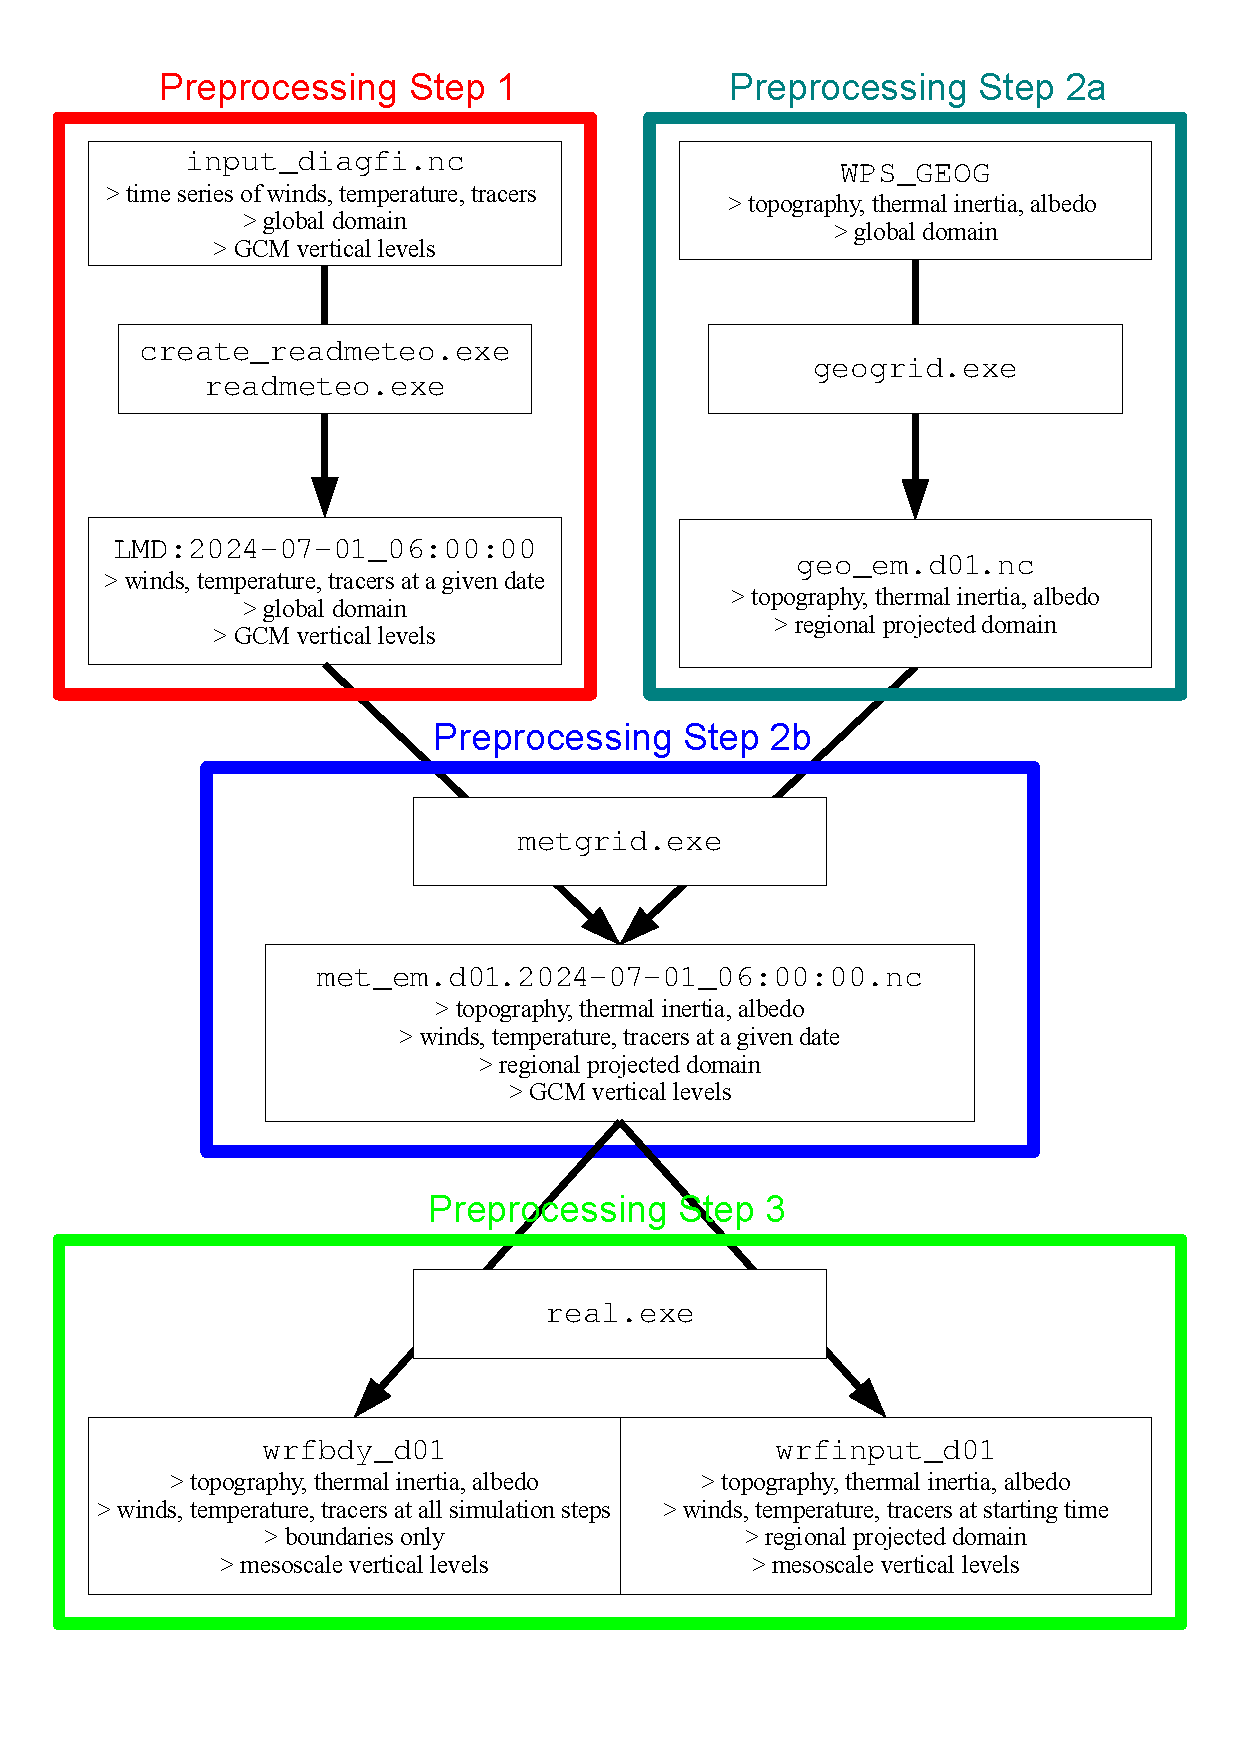
\includegraphics[width=0.99\textwidth]{diagramme.pdf} 
\caption{\label{preproc} The details of preprocessing steps and their related software and inputs/ouputs}
\end{figure}
\end{center}

%\sk
\subsection{Step 1: Running the GCM and converting data}\label{gcmini}

\sk
Here we assume that the user has chosen a given Martian sol or $L_s$ on which to start the mesoscale simulation. As already mentionned in section~\ref{namelist}, the file \ttt{\$MMM/SIMU/calendar} reproduced in appendix can help with this choice (i.e. sol$\rightarrow$$L_s$$\rightarrow$mesoscale date and vice-versa). In addition, the user has to check in the \ttt{calendar} file which sol is before the one wanted for simulation start and has $99$ in the first column: such sols are the ones for which an initial starting file for the GCM is available. Then the number of GCM simulated days \ttt{nday} in \ttt{\$MESO/LMDZ.MARS/myGCM/run.def} must be set accordingly: suppose you want to start a mesoscale simulation at sol~9 during 4~sols, then according to the \ttt{calendar} file, sol~8 is the closest file before sol~9 to be in the database, so \ttt{nday} must be at least~$5$. For optimal forcing at the boundaries, we advise you to write the meteorological fields to the \ttt{diagfi.nc} file at least each two hours, or ideally each hour\footnote{The parameter \ttt{interval\_seconds} in \ttt{namelist.wps} (see section~\ref{wps}) has to be set accordingly.}, i.e. \ttt{ecritphy} is respectively~$80$ or~$40$ in \ttt{\$MESO/LMDZ.MARS/myGCM/run.def}. Eventually the GCM run can be launched using the following commands and should produce a netCDF data file named \ttt{diagfi.nc}:

\begin{verbatim}
cd $MESO/LMDZ.MARS/myGCM
[edit run.def, in particular to modify nday]
./launch_gcm    ## answer: your desired starting sol for the simulations
\end{verbatim}

	%\mk
	%\marge An example of input meteorological file	 
	%\ttt{diagfi.nc} file can be downloaded
	%at \url{http://web.lmd.jussieu.fr/~aslmd/LMD_MM_MARS/diagfi.nc.tar.gz}.
	%%
	%Please deflate the archive and copy the \ttt{diagfi.nc} file
	%in \ttt{\$MESO/TMPDIR/GCMINI}.
	%%
	%Such a file can then be used to define the initial
	%and boundary conditions, and we will go 
	%through the three preprocessing steps.

\sk
Once the GCM simulations are finished, programs in the \ttt{PREP\_MARS} directory allow the user to convert the data from the NETCDF \ttt{diagfi.nc} file into separated binary datafiles\footnote{If the fields \ttt{emis}, \ttt{co2ice}, \ttt{q01}, \ttt{q02}, \ttt{tsoil} are missing in the \ttt{diagfi.nc} file, those are replaced by respective default values $0.95$, $0$, $0$, $0$, tsurf.} for each date contained in \ttt{diagfi.nc} and formatted for the preprocessing programs at step 2. These programs can be executed by the following commands; if everything went well with the conversion, the directory \ttt{\$MESO/TMPDIR/WPSFEED} should contain files named \ttt{LMD:*}. 

\begin{verbatim}
cd $MMM/your_install_dir/PREP_MARS
echo 1 | ./create_readmeteo.exe     # drop the "echo 1 |" if you want control
./readmeteo.exe < readmeteo.def
\end{verbatim}

\sk
\subsection{Step 2: Interpolation on the regional domain}\label{wps}

\sk
\paragraph{Step 2a} In the \ttt{WPS} directory, the \ttt{geogrid.exe} program allows you to define the mesoscale simulation domain, to horizontally interpolate the topography, thermal inertia and albedo fields at the domain resolution and to calculate useful fields such as topographical slopes. Please execute the commands:

\begin{verbatim}
cd $MMM/your_install_dir/WPS
ln -sf $MMM/TESTCASE/namelist.wps .   # test case (or use your customized file)
./geogrid.exe
\end{verbatim}

The result of \ttt{geogrid.exe} -- and thus the definition of the mesoscale domain -- can be checked in the NETCDF file \ttt{geo\_em.d01.nc} e.g. with topographical fields \ttt{HGT\_M} \ttt{HGT\_U} \ttt{HGT\_V} (using for instance \ttt{ncview}, or your favorite graphical interface for netCDF files, or python-based scripts as in section~\ref{postproc}). If you are unhappy with the results or you want to change the location of the mesoscale domain on the planet, the horizontal resolution, the number of grid points \ldots, please modify the parameter file \ttt{namelist.wps}, content thereof is reproduced/commented on the next page\footnote{You may find the corresponding file in \ttt{\$MMM/SIMU/namelist.wps\_example}.}, and execute again \ttt{geogrid.exe}. 

\begin{finger}
\item No input meteorological data are actually needed to execute \ttt{geogrid.exe}. This step~2a can be done e.g. before step~1. It is probably a good idea to prepare step~2 by choosing the mesoscale simulation domain while GCM computations being performed during step~1. 
\item More details about the database and more options of interpolation could be found in the file \ttt{geogrid/GEOGRID.TBL} (for advanced users only).
\item Two examples of \ttt{namelist.wps} parameters are given in Figure~\ref{vallespolar} with resulting domains.
\end{finger}

\footnotesize
\codesource{namelist.wps_example}
\normalsize

\begin{figure}[h!] 
\begin{center}
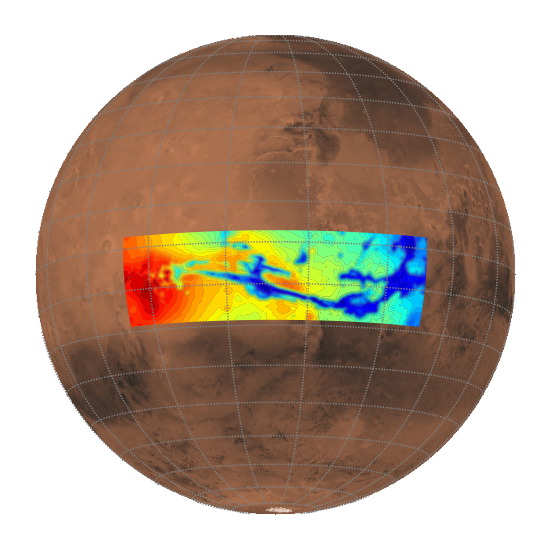
\includegraphics[width=0.48\textwidth]{valles.png}
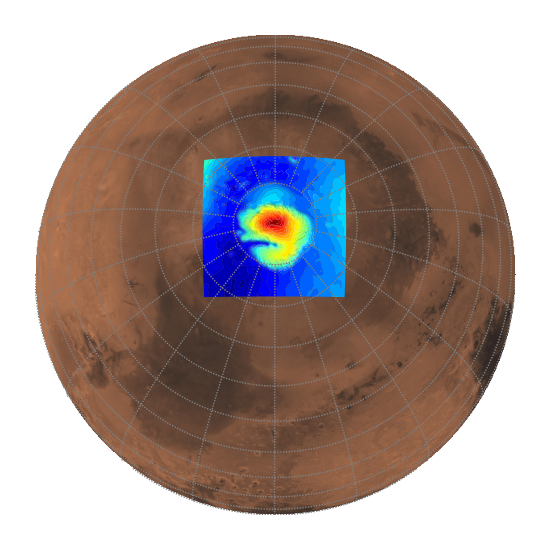
\includegraphics[width=0.48\textwidth]{LMD_MMM_d1_20km_domain_100.png} 
\end{center}
\caption{\label{vallespolar} (Left plot) An example of mercator domain in the Valles Marineris region as simulated by \textit{Spiga and Forget} [2009, their section 3.3]: relevant parameters in \ttt{namelist.wps} are: \ttt{e\_we = 401}, \ttt{e\_we = 121}, \ttt{dx = 12000}, \ttt{dy = 12000}, \ttt{map\_proj = 'mercator'}, \ttt{ref\_lat = -8}, \ttt{ref\_lon = -68}. (Right plot) An example of north polar domain with stereographical projection: relevant parameters in \ttt{namelist.wps} are: \ttt{e\_we = 117}, \ttt{e\_we = 117}, \ttt{dx = 20000}, \ttt{dy = 20000}, \ttt{map\_proj = 'polar'}, \ttt{ref\_lat = 90}, \ttt{ref\_lon = 0.1}, \ttt{truelat1  =  90}, \ttt{stand\_lon =  0.1}.}
\end{figure}

\sk
The input datasets for topography and soil properties can be set in \ttt{namelist.wps} through the keyword \ttt{geog\_data\_res}. Possible choices are:
\begin{citemize}
\item \ttt{'gcm'}: coarse-resolution datasets;
\item \ttt{'32ppd'}: coarse-resolution datasets, but 32ppd MOLA topography;
\item \ttt{'64ppd'}: fine-resolution datasets: TES albedo \& thermal inertia, 64ppd MOLA topography;
\item \ttt{'64ppd\_noHRti'}: fine-resolution datasets, but coarse-resolution thermal inertia;
\item \ttt{'32ppd\_HRalb'}: fine-resolution albedo, coarse-resolution thermal inertia, 32ppd topography.
\end{citemize}
The corresponding dataset must have been built in the \ttt{WPS\_GEOG} folder previously (see section~\ref{wpsgeog}).

\sk
\paragraph{Step 2b} Once the \ttt{geo\_em} file(s) are generated, the \ttt{metgrid.exe} program performs a similar horizontal interpolation of the meteorological fields to the mesoscale domain as the one performed by \ttt{geogrid.exe} for the surface data (interpolation options can be modified by advanced users in \ttt{metgrid/METGRID.TBL}). Then the program writes the results in \ttt{met\_em} files and also collects the static fields and domain parameters included in the \ttt{geo\_em} file(s). If everything went well with the commands below, the directory \ttt{\$MESO/TMPDIR/WRFFEED/current} should contain \ttt{met\_em.*} files.

\begin{verbatim}
cd $MMM/your_install_dir/WPS
mkdir WRFFEED/current
./metgrid.exe
\end{verbatim}

\sk
\subsection{Step 3: Vertical interpolation on mesoscale levels}\label{real.exe}

\sk
The last preprocessing step before being able to run the mesoscale simulation at step~4 is to execute \ttt{real.exe} to perform the interpolation from the vertical levels of the GCM to the vertical levels defined in the mesoscale model. This program also prepares the final initial state for the simulation in files named \ttt{wrfinput} and the boundary conditions in files named \ttt{wrfbdy}. To successfully execute \ttt{real.exe}, you need the \ttt{met\_em.*} files and the \ttt{namelist.input} file to be in the same directory as \ttt{real.exe}. Parameters in \ttt{namelist.input} which controls the behavior of the vertical interpolation are those labelled with \ttt{(p3)} in the detailed list introduced in chapter~\ref{zeparam}. 

\begin{verbatim}
cd $MMM/TESTCASE   ## or anywhere you would like to run the simulation
ln -sf $MESO/TMPDIR/WRFFEED/current/met_em* .
./real.exe
\end{verbatim}

\sk
The final message of the \ttt{real.exe} should claim the success of the processes and you are now ready to launch the integrations of the LMD Martian Mesoscale Model with the \ttt{wrf.exe} command as in section \ref{sc:arsia}.

\sk
\begin{finger}
\item \textbf{ When you modify either \ttt{namelist.wps} or \ttt{namelist.input}, make sure that the common parameters are exactly similar in both files (especially when running nested simulations) otherwise either \ttt{real.exe} or \ttt{wrf.exe} command will exit with an error message. Obviously the dates sent to \ttt{launch\_gcm} and set in both \ttt{namelist.input} and \ttt{namelist.wps} should be consistent too. }
\end{finger}

\clearemptydoublepage


ok_guide=y
# guidage sur niveaux mod�le (y) ou standard
guide_modele=y
# inversion de l'ordre des niveaux verticaux
ok_invertp=y
ncep=y
 ######################################
 #### guidage de u #####
 guide_u=y
 ######################################
 #### guidage de v #####
 guide_v=y
 ######################################
 #### guidage de T #####
 guide_T=y
 ######################################
 #### guidage de P #####
 guide_P=n
 ######################################
 #### guidage de Q (hr=y:hum.rel,n:hum.spec) #####
 guide_Q=n
 guide_hr=n
 ######################################
 ## guidage dans la couche limite
 guide_BL=n
 ######################################
ini_anal=n
tau_min_u=0.04166667
tau_max_u=0.125
tau_min_v=0.04166667
tau_max_v=0.125
tau_min_T=0.04166667
tau_max_T=10.
tau_min_Q=0.2
tau_max_Q=10.
# gamma limit�
gamma4=n

\chapter{Advanced simulations}\label{advance}

\vk
In this chapter, advice to perform more sophisticated simulations is provided to advanced users. 

\mk
\section{Running nested simulations}\label{nests}

\paragraph{Preparing namelist.input} For simulations with \ttt{max\_dom} nested domains, \ttt{max\_dom} parameters must be set wherever there is a ``," in the \ttt{namelist.input\_full} template in chapter~\ref{zeparam}. Specific parameters for nested simulations are labelled with \ttt{(n)} in this \ttt{namelist.input} template (see e.g. categories \ttt{\&time\_control}, \ttt{\&domains} and \ttt{\&bdy\_control}). To help you with filling the \ttt{namelist.input} file for a nested simulation, a commented example is given below. 

\vskip -0.4cm
\scriptsize
\codesource{namelist.input_nests}
\normalsize

\paragraph{Preparing namelist.wps} As is the case for single-domain simulations, the common parameters in the two files \ttt{namelist.input} and~\ttt{namelist.wps} must be exactly similar. Similarly to single-domain simulations, an automated generation of \ttt{namelist.wps} from \ttt{namelist.input} is provided in the \ttt{runmeso} script. If you do not use \ttt{runmeso} to generate the \ttt{namelist.wps} file, please bear in mind that in this file, dates are different for the parent domain and the child domains, since boundary conditions are needed only for the parent domain while initial conditions are needed for all domains. The \ttt{namelist.wps} file associated to the previously described \ttt{namelist.input} file is given below\footnote{You may find \ttt{namelist.input\_nests} and \ttt{namelist.wps\_nests} in \ttt{\$MMM/SIMU}.} and corresponds to a nested simulation in the Hellas Planitia region (Figure~\ref{nesteddomains}). Note that map projection is similar in all nests.

\vskip -0.2cm
\scriptsize
\codesource{namelist.wps_nests}
\normalsize

\begin{center} 
\begin{figure}[h!]
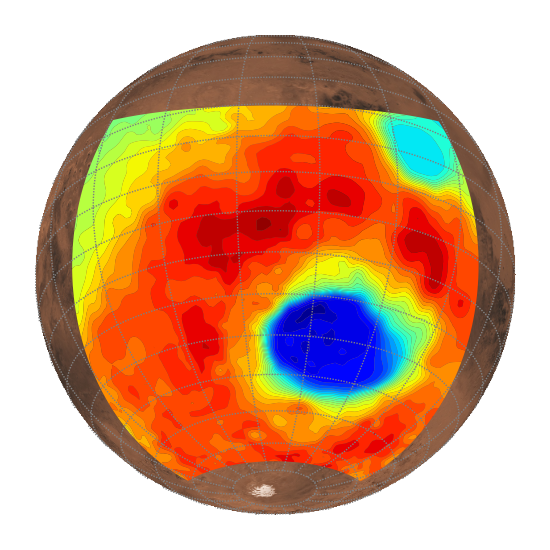
\includegraphics[width=0.33\textwidth]{LMD_MMM_d1_63km_domain_100.png} 
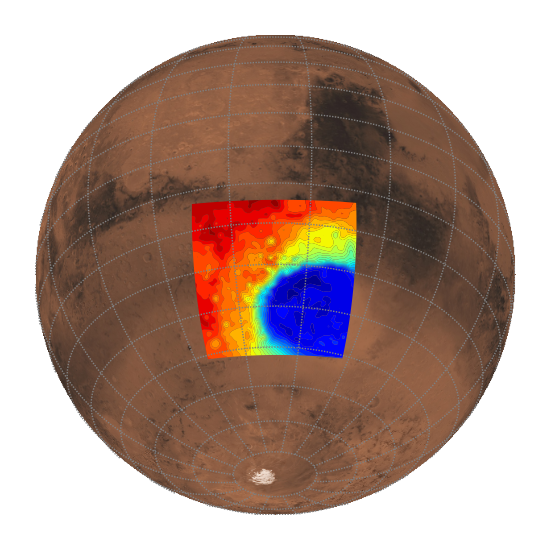
\includegraphics[width=0.33\textwidth]{LMD_MMM_d2_21km_domain_100.png}
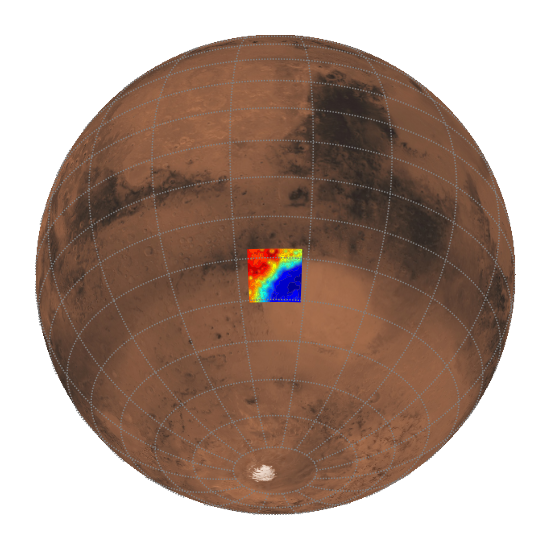
\includegraphics[width=0.33\textwidth]{LMD_MMM_d3_7km_domain_100.png}
\caption{\label{nesteddomains} Domains for a nested mesoscale simulations in Hella Planitia defined by \ttt{namelist.wps\_nests}. From left to right, ``parent" domain i.e. nest number~$1$ (horizontal resolution $63$~km), ``child" domain i.e. nest number~$2$ (horizontal resolution $21$~km), ``grandchild" domain i.e. nest number~$3$ (horizontal resolution $7$~km).}
\end{figure}
\end{center}

\paragraph{Preparing callphys.def} If you run a simulation with, say, $3$ domains, please ensure that you defined three files \ttt{callphys.def}, \ttt{callphys\_d2.def} and \ttt{callphys\_d3.def} (one per nest). If needed, different settings for physical parameterizations can be made in each nest; usually all settings in these files are similar, except \ttt{iradia} (so that differences in dynamical timesteps between nests can be potentially impacted to \ttt{callphys*.def} in order to synchronize radiative transfer call).

\paragraph{Compiling} Use the command \ttt{makemeso} and specify the number of domains and dimensions set in \ttt{namelist.input} (as far as the horizontal grid is concerned, answers to \ttt{makemeso} shall refer to the values of \ttt{e\_we} and \ttt{e\_sn} for the parent domain). This is done automatically of course if you use \ttt{runmeso} which reads the information in \ttt{namelist.input}.

\paragraph{Running} If grid nesting and parallel computing are used, no more than~$4$ processors can be used. If the nested simulation is unstable, try a single-domain simulation with the parent domain and choose best parameters for stability (e.g., \ttt{time\_step}), then add a first nested domain, and start again stability tests and investigations, etc.

\paragraph{Inputs/outputs} Defining several domains yield one output per domain: e.g. for three domains \ttt{geogrid.exe} yields \ttt{geo\_em.d01.nc}, \ttt{geo\_em.d02.nc}, \ttt{geo\_em.d03.nc}\ldots; \ttt{real.exe} yields \ttt{wrfinput\_d01}, \ttt{wrfinput\_d02}, \ttt{wrfinput\_d03}, \ldots; \ttt{wrf.exe} yields \ttt{wrfout\_d01*}, \ttt{wrfout\_d02*}, \ttt{wrfout\_d03*}, \ldots   

\paragraph{Useful remarks} The model presently supports 3 nests, but more nests can be included by adaptating \ttt{runmeso} and the following files: 
%\scriptsize
\begin{verbatim}
$LMDMOD/LMD_MM_MARS/SRC/WRFV2/call_meso_inifis3.inc
$LMDMOD/LMD_MM_MARS/SRC/WRFV2/call_meso_physiq3.inc
$LMDMOD/LMD_MM_MARS/SRC/WRFV2/mars_lmd/libf/duplicate3
$LMDMOD/LMD_MM_MARS/SRC/WRFV2/mars_lmd/libf/generate3
$LMDMOD/LMD_MM_MARS/SRC/WRFV2/mars_lmd/makegcm*  ## search for 'nest'
\end{verbatim}
%\normalsize

\mk
\section{Running simulations with tracers}

\paragraph{Preparing namelist.input} The default behavior of the model is to include no transported tracer by the dynamics. This corresponds to \ttt{mars=0} in \ttt{namelist.input} (or the absence of parameter \ttt{mars} from the user's namelist). To compute the water cycle in the LMD Martian Mesoscale Model, simply set \ttt{mars=1} in \ttt{namelist.input} (category \ttt{\&physics}). This will add one tracer for water vapor and one tracer for water ice in the model's computations and outputs. To compute a mesoscale simulation with one simple transported dust bin (with typical characteristics), set \ttt{mars=2} in \ttt{namelist.input}.

\paragraph{GCM inputs} For water cycle simulations (\ttt{mars=1}), the GCM runs used to build initial and boundary conditions for the mesoscale model must also include water tracers. This is done by default in parameter files in \ttt{\$MESO/LMDZ.MARS/myGCM}, compiler wrapper \ttt{\$MESO/LMDZ.MARS/compile} and the database of start files \ttt{STARTBASE\_64\_48\_32\_t2}.

\paragraph{Preparing callphys.def} It is important to set \ttt{callphys.def} in accordance with the option chosen for the keyword \ttt{mars} in \ttt{namelist.input}. For instance, for water cycle simulations (\ttt{mars=1}), the following settings must be changed in \ttt{callphys.def}: \ttt{tracer}, \ttt{sedimentation}, \ttt{iceparty}, \ttt{water} shall be \ttt{T}. An example file is \ttt{\$MMM/SIMU/DEF/REF\_ARTICLE/callphys.def.mars1}.

\paragraph{Compiling} It is key to recompile the LMD Martian Mesoscale Model with \ttt{makemeso} each time the number of transported tracers has changed, which would most often be the case if you modify \ttt{mars} in \ttt{namelist.input}. The right number of tracers corresponding to the \ttt{mars} case you are setting must be specified when answering questions to the \ttt{makemeso} script. This is of course automatically done if you use \ttt{runmeso} which reads the information in \ttt{namelist.input}.

\paragraph{Inputs/outputs} Additional fields corresponding to tracer mixing ratios (e.g. \ttt{QH2O} for water vapor) are automatically output in \ttt{wrfout*} files if a different option than~\ttt{0} is used for the \ttt{mars} keyword. Note that when a large number of tracers is set, output files might grow very large quickly after the mesoscale simulation is launched.

\paragraph{Test case} A good test case consists in coming back to the Arsia simulation described in section~\ref{sc:arsia} and activate the water cycle. Add \ttt{mars=1} to \ttt{namelist.input}, change \ttt{callphys.def} as described previously. Launch \ttt{runmeso} and choose \ttt{3} (i.e. recompile the model, run \ttt{real.exe} so that initial and boundary conditions for water are included, eventually run \ttt{wrf.exe}). Check for tracer fields in output files \ttt{wrfout*}. 

\mk
\section{Running Large-Eddy Simulations}

\paragraph{Prerequisites} Large-Eddy Simulations are very specific applications of the LMD Martian Meso\-scale Model which allow the user to simulate boundary layer turbulent convection in idealized conditions at fine spatial and temporal resolution. We recommend to read section 3.4 of \textit{Spiga and Forget} [2009] and the first three sections of \textit{Spiga et al.} [2010]\nocite{Spig:10bl}.

\paragraph{Preparing namelist.input} A typical parameter file \ttt{namelist.input\_les} is given in what follows (and could be found in \ttt{\$MMM/SIMU}). Settings specific to Large-Eddy Simulations are referred to as \ttt{LES}. The main differences with regular mesoscale simulations are the following: 
\begin{citemize}
\item the duration of simulation is specified in seconds, 
\item model top is specified as altitude above surface, 
\item the dynamical timestep and the spatial resolutions are much smaller,
\item an additional \ttt{isfflx} keyword defines surface forcings (\ttt{1} is recommended),
\item albedo and thermal inertia have to be set with uniform user-defined values,
\item idealized wind profile is assumed,
\item \ttt{\&dynamics} keywords are adapted to small-scale diffusion,
\item periodic boundary conditions are set for the horizontal grid.
\end{citemize}

\scriptsize
\codesource{namelist.input_les}
\normalsize

%\vskip 0.4cm
\newpage

\paragraph{Preparing callphys.def} It is essential that \ttt{calldifv} is set to \ttt{T} and \ttt{calladj} is set to \ttt{F} for Large-Eddy Simulations. Generally \ttt{iaervar} is set to \ttt{1} so that the (uniform) opacity in the domain can be set by adding a text file named \ttt{dustopacity.def} with the chosen value for opacity in it.

\paragraph{Compiling} The dynamical core used for Martian Large-Eddy Simulations is different than usual mesoscale simulations; it is based on WRF v3 instead of WRF v2. The first time the model is compiled, the user has to install it by typing the following commands:
\begin{verbatim}
cd $MMM/SRC/LES
./LMD_LES_MARS_install
cd $MMM
\end{verbatim}
The compilation of the Large-Eddy Simulations model is carried out through the command: 
\begin{verbatim}
makemeso -c les 
\end{verbatim}
This creates a new compilation folder with prefix \ttt{les} in which the executables can be found once the model is compiled. Answers to \ttt{makemeso} must be compliant with settings in \ttt{namelist.input}.

\paragraph{Inputs/outputs} Large-Eddy Simulations need four input files \ttt{input\_coord}, \ttt{input\_sounding}, \ttt{input\_more}, \ttt{input\_therm} which define initial pressure, temperature, density, winds profiles at the location/season for which simulations are run, along with information about this location/season. Typical files are available upon request, or you might simply build your own profiles using the Mars Climate Database (see the sample \ttt{scilab} script \ttt{wrf\_sounding.sci} in \ttt{\$MMM/SIMU/RUN}). Examples for \ttt{input\_*} files are provided in \ttt{\$MMM/SRC/LES/modif\_mars/DEF} and correspond to the cases run in the study by \textit{Spiga et al.} [2010].

%% IMPORTANT IMPORTANT
%% now python inimeso.py in UTIL/PYTHON

\begin{citemize}
\item \ttt{input\_coord} contains longitude, latitude, $L_s$ and local time;
\item \ttt{input\_sounding} contains (first line) near-surface pressure (mbar), potential temperature, a dummy value; and (subsequent lines) altitudes above MOLA zero datum, potential temperatures, dummy value, zonal wind component, meridional wind component;
\item \ttt{input\_more} contains on the same line altimetry and surface temperature;
\item \ttt{input\_therm} contains lines with corresponding values for (from left column to right column)~$R$, $c_p$, pressure, density, temperature.
\end{citemize}

\paragraph{Running} Large-Eddy Simulations are not supported by \ttt{runmeso}. After compiling the model with the command \ttt{makemeso -c les}, please copy the executables \ttt{ideal.exe} and \ttt{wrf.exe} from the compilation directory \ttt{\$MMM/les*} towards your simulation directory where the \ttt{input\_*} files are located. Running \ttt{ideal.exe} would generate the initial state \ttt{wrfbdy\_d01} from the profiles provided in the \ttt{input\_*} files, then running \ttt{wrf.exe} would launch the model's integrations.


%%% le modele supporte en fait 5 nests
%%% ne pas oublier que mars doit etre dupliquee dans la namelist...


%\mk
%\section{Idealized test cases} [such as GW case]

%ze_hill ???
%version without physics ???


\mk
\section{Running simulations with the new physical parameterizations}

\sk
Using the most recent physical parameterizations means using a version of the LMD Martian Mesoscale Model that is still under development (thus experimental). It is therefore recommended to contact developers to run simulations in this mode. Reference setting files are located in \ttt{MESOSCALE/LMD\_MM\_MARS/SIMU/DEF/newphys\_THARSIS\_WATER}.

\sk
For advanced users who learnt with the LMD team how to use the new physical parameterizations, here are a few differences with the physical parameterizations natively provided with the LMD Martian Mesoscale Model that must be kept in mind
\begin{finger}
\item a folder \ttt{LMDZ\_MARS} containing the latest sources of the Mars LMD GCM must be located in the same repository which contains \ttt{MESOSCALE} (easy to do with SVN)
\item GCM runs used to produce initial and boundary conditions for the mesoscale model must be done in \ttt{MESOSCALE/LMDZ.MARS.new}
\item \ttt{makemeso} must be used with option \ttt{-p}
\item the \ttt{callphys.def} file is different
\item modifying the \ttt{datafile.h} is not necessary anymore, this can be done in \ttt{callphys.def}
\item an additional \ttt{run.def} file is needed
\item in \ttt{namelist.input}, the soil model must set to 18 levels
\item in \ttt{namelist.input}, the 6th order small scale diffusion must be set to 0 (i.e. \ttt{diff\_6th\_opt = 0}) if the resolution is small ($<10$~km)
\item additional \ttt{mars} modes can be accessed (e.g. for interactive dust or the radiative effect of clouds)
%\item if \ttt{init\_TI} is modified, \ttt{real.exe} must be run again (because of subsurface modeling)
\item a varying map for surface roughness~$z_0$ can be used -- or a constant value can be set with \ttt{init\_Z0} in \ttt{namelist.input} (if there is a problem, the old reference of 1cm is chosen)
\item (starting from version \ttt{r1038}) the model does not need to be recompiled if the number of tracers is changed
\item (starting from version \ttt{r1214}) the model does not need to be recompiled if the number of horizontal grid points or the number of processors is changed
\item (prior to version \ttt{r1247}) the number of scatterers must be given when compiling, standard simulation uses 1 scatterer (2 is used for radiatively active water ice clouds)
\item (starting from version \ttt{r1247}) the model does not need to be recompiled if the number of scatterers is changed
\item (starting from version \ttt{r1272}) the model does not need to be recompiled if the number of vertical levels is changed
\end{finger}

For nested runs, all versions posterior to \ttt{r1027} are broken. However, the interface between the WRF dynamical core and the LMD physical parameterizations has been significantly improved in \ttt{r1243}, which fixes nesting runs and simplifies restart runs. Those improvements remain to be extensively tested more extensively, but getting an operational model with nesting and restart runs will only require now minor adjustments that will be committed in subsequent revisions of the model.

%% r1199 MESOSCALE. possibility to experiment simulations with Wee et al. 2012 changes in initialization (more consistent handling of hypsometric equation)
%% run.def different if callphys different for nests

%%% Here is how to output near-surface diagnostics
%- Look for n_out in physiq.F this will lead you to a few lines of codes that will allow you to output near-surface diagnostics
%- Change n_out to a value of 2
%- A few lines below change z_out and make it equal to [1.6,0.5]
%Now this is OK for physics, but you have to make this available in the dynamical outputs of WRF
%Go to the mesoscale sources, then in Registry find Registry.EM
%then following the example of this kind of line
%state  real  ALBBARE   ij   misc  1  -  rhd   "ALBBARE"   "SOIL ALBEDO"                     ""        #SAVEMARS2 albedodat
%add this
%state  real  TVIK   ij   misc  1  -  rhd   "TVIK"   "temperature at 1.6m"     "K"       #SAVEMARS2 T_out1
%Then proceed through a full recompile of the mesoscale model from scratch Here is how to output near-surface diagnostics
%- Look for n_out in physiq.F this will lead you to a few lines of codes that will allow you to output near-surface diagnostics
%- Change n_out to a value of 2
%- A few lines below change z_out and make it equal to [1.6,0.5]
%Now this is OK for physics, but you have to make this available in the dynamical outputs of WRF
%Go to the mesoscale sources, then in Registry find Registry.EM
%then following the example of this kind of line
%state  real  ALBBARE   ij   misc  1  -  rhd   "ALBBARE"   "SOIL ALBEDO"                     ""        #SAVEMARS2 albedodat
%add this
%state  real  TVIK   ij   misc  1  -  rhd   "TVIK"   "temperature at 1.6m"     "K"       #SAVEMARS2 T_out1
%Then proceed through a full recompile of the mesoscale model from scratch 

\sk
A fully functional modeling architecture with \ttt{LMD\_MM\_MARS} and the new physical parameterizations (as well as the \ttt{LMDZ\_MARS} Global Climate Model used to initialize the mesoscale simulations) can be downloaded and compiled using the \ttt{meso\_install.sh} script: \url{http://svn.lmd.jussieu.fr/Planeto/trunk/MESOSCALE/LMD_MM_MARS/SIMU/meso_install.sh}. The \ttt{NETCDF} environment variable shall be positioned. The \ttt{meso\_install.sh} script only works on the IPSL \ttt{ciclad} computing cluster with compiler ifort; it shall be used as a template for other environments (or manually installing the architecture step-by-step). Options in the \ttt{meso\_install.sh} script can be displayed with the \ttt{-h} option.

%I think the main point is to change CICLAD for a name representative of your local cluster, and then creates a arch file analogous to what is done for arch_CICLADifort, but adapted to your local cluster

%declare -x WHERE_MPI=/usr/lib64/openmpi/1.6.5-ifort/bin/
%declare -x NETCDF=/opt/netcdf3/ifort
%declare -x NCDFLIB=$NETCDF/lib
%declare -x NCDFINC=$NETCDF/include
%### pour fcm nouvelle version du GCM
%declare -x PATH=~millour/FCM_V1.2/bin/:$PATH
%## + mettre ./ dans PATH

%r1613 (or slightly before) use of -p mars_lmd_new



\clearemptydoublepage

\chapter{Post-processing}\label{postproc}

\vk
In this chapter, the user is introduced to the principles of choosing the outputs of the LMD Martian Mesoscale Model. Elements about post-processing (interpolation, graphics) are also proposed here, although it is obviously left to the user to choose and develop its own tools to analyze the results of LMD Martian Mesoscale Model computations.

\mk
\section{Controlling which fields to output in \ttt{wrfout} files}

\sk
All non-local variables communicated within subroutines and functions in the WRF dynamical core are declared in a text file named \ttt{Registry.EM} located in \ttt{\$MMM/SRC/WRFV2/Registry}. In this file, each useful variable is declared through a one-line instance organized as follows:

\scriptsize
\begin{verbatim}
state  real  PSFC  ij  misc  1  -  i01rh  "PSFC"  "SFC PRESSURE"  "Pa"
\end{verbatim}
\normalsize

\sk
The fields which appears in \ttt{wrfout*} output files feature an \ttt{h} (which stands for history) in the 8th column. If you do not want the field to appear in \ttt{wrfout*} files, simply remove the letter \ttt{h} from the group of letters in the 8th column. If you want the field to appear in \ttt{wrfout*} files, simply add the letter \ttt{h} in the group of letters in the 8th column.  

\sk
It is also possible to output fields which are present only in the physical computations, i.e. appearing in \ttt{\$MMM/SRC/WRFV2/mars\_lmd/libf/phymars/physiq.F}. The method is simple. Assume you would like to output in the \ttt{wrfout*} files a 3D field named \ttt{zdtnirco2} and a 2D field named \ttt{qsurfice} in \ttt{physiq.F} with the new names \ttt{HR\_NIR} and \ttt{QSURFICE}. All you have to do is add the following lines to \ttt{Registry.EM} (see also examples around lines \ttt{75-120}). For 2D [3D] files the 4th column must be \ttt{ij} [\ttt{ikj}] and the 12th column \ttt{\#SAVEMARS2} [\ttt{\#SAVEMARS3}].

\scriptsize
\begin{verbatim}
state  real  HR_NIR  ikj  misc  1  -  rhd  "HR_NIR"  "HEATING RATE nirco2"  "K/s"  #SAVEMARS3  zdtnirco2
state  real  QSURFICE  ij  misc  1  -  rhd  "QSURFICE"  "WATER ICE AT SURFACE"  "kg m-2"  #SAVEMARS2  qsurfice
\end{verbatim}
\normalsize

\sk
Each change in \ttt{Registry.EM} must be followed by a complete recompilation because the model variables have changed. Whether you use \ttt{makemeso} or \ttt{runmeso}, use the option \ttt{-f} to force recompiling with a new/updated list of variables.
%%%% now obsolete ! remove Registry and recompile, or use fresh start (-f).

\sk
\begin{finger}
\item IMPORTANT: Each compilation directory \ttt{your\_compdir} in \ttt{\$MMM} (e.g. \ttt{g95\_32\_single}) has its own copy of \ttt{Registry.EM} in \ttt{your\_compdir/WRFV2/Registry}. This is the file that has to be modified. The file \ttt{\$MMM/SRC/WRFV2/Registry/Registry.EM} should not be modified: it is the reference file that is copied when the compilation directory is built by the \ttt{copy\_model} script (cf. section~\ref{sc:makemeso}).
\end{finger}

\mk
\section{Interpolating outputs on altitude and pressure levels}

\sk
The fields output in \ttt{wrfout*} files are given for each grid point and model level. A vertical interpolation has to be performed to get those fields either in altitude or pressure levels. In addition, perturbation potential temperature \ttt{T}, x-component wind \ttt{U} and y-component \ttt{V} are output instead of the more informative (meteorologically-speaking) temperature \ttt{tk}, zonal wind \ttt{Um} and meridional wind \ttt{Vm}. This is why we developed a program named \ttt{api} (Altitude and Pressure Interpolator) which performs the tasks to convert the netCDF \ttt{wrfout*} files into another netCDF file featuring more useful fields to make plots and analyze the Martian mesoscale meteorology.

\sk
The source files for \ttt{api} are located in \ttt{\$MMM/SRC/POSTPROC/}. The program \ttt{api.F90} has to be compiled with the \ttt{comp\_api} command (which must be edited first, to uncomment the line corresponding to the Fortran compiler you are used to). Then the user has to fill in the parameter file \ttt{namelist.api} before launching the interpolator through the command \ttt{api}. A commented template for \ttt{namelist.api} is given below (this examples and many others can be found in \ttt{\$MMM/SRC/POSTPROC/}). The calculations might be long if you are requesting many fields and many interpolation levels. In the example below, temperature, meteorological winds and vertical velocity are interpolated at~$50$~m above the local surface. The results are output in a netCDF file having the same name as the input \ttt{wrfout*} files, with an additional suffix which depends on the chosen interpolation method.

\scriptsize
\codesource{namelist.api}
\normalsize

\mk
\section{Generating maps for winds and meteorological fields simulated by the model}\label{plots}

\sk
%This section does not replace the need for you to develop your own plotting tools to suit your needs, which should be not too difficult. 
The model outputs, as well as the results of \ttt{api} interpolations, are written using the netCDF format which can be read by most software with graphical capabilities. For a quick inspection of model results (especially for checking model outputs while the model is running), we recommend using \ttt{ncview}; for simple manipulations of netCDF files (e.g. concatenation, difference, extraction, \ldots), we recommend using commands from the \ttt{nco} package (see chapter~\ref{install} for website links). Graphical routines based on \ttt{idl}, \ttt{ferret} and \ttt{grads} can be made available upon request (as is, i.e. undocumented yet commented scripts). Successful reading/plotting of the LMD Martian Mesoscale Model outputs on \ttt{matlab}, \ttt{octave}, \ttt{idv} are also reported. It is possible to import the model's outputs to Geographical Information System (GIS) such as \ttt{arcgis}\footnote{\ttt{idl}, \ttt{matlab} and \ttt{arcgis} are neither open-source nor free.}. Since 2012, we developped our own tool named \ttt{PLANETOPLOT} based on \ttt{Python}. More information can be found here: \url{http://www.lmd.jussieu.fr/~aslmd/planetoplot}.

%\sk
%\subsection{Python scripts}
%
%\sk
%Powerful scripts based on \ttt{python+numpy+matplotlib} have been developed to obtain plots from the mesoscale model outputs. All figures in this user manual are based on the script \ttt{pp.py}. This script can be obtained with the commands: \ttt{cd \$MESO ; cd .. ; svn update UTIL ; cd UTIL/PYTHON}. It is required that \ttt{python} and numerical/graphical librairies (\ttt{numpy}, \ttt{scipy}, \ttt{matplotlib}, \ttt{basemap}, \ttt{netcdf}) are installed on your system. Perhaps the simplest way to do so is to install the user-friendly complete python distribution \ttt{epd} (cf. link in chapter~\ref{install} and readme file \ttt{UTIL/PYTHON/README.INSTALL}). 
%
%\sk
%One of the advantages of an approach using \ttt{python}, apart from its open-source philosophy and the abundant online documentation, is that it allows, in a common framework, for scripting with various options, integrating Fortran routines, manipulating arrays, making plots with various map projections. This is exemplified by the \ttt{pp.py} script. It can both perform interpolation with \ttt{api} for the level requested by the user then generate a map, all that in one simple command line. For instance, Figures~\ref{arsia} in chapter~\ref{compile} has been generated by the following two commands\footnote{The first plot can also be obtained by the command \ttt{domain.py -f name\_of\_file}}:
%
%\begin{verbatim}
%pp.py -f wrfout_d01_2024-01-17_02:00:00 -p ortho -b vishires --title ""
%pp.py -f wrfout_d01_2024-01-17_02:00:00 -i 4 -l 0.01 -v HGT -W -s 2 \
%      --time 1 --axtime lt -m -1500. -M 20000. --div 20 -c nobar -z 25
%\end{verbatim}
%
%\sk
%Many options are implemented in our \ttt{pp.py} script. The information on the existing options to~\ttt{pp.py} can be obtained by typing \ttt{pp.py -h} (cf. next page). Examples on how to use the \ttt{pp.py} script can be found in \ttt{UTIL/PYTHON/README.PP}. The script can also be edited to suit your needs if the desired option does not exist.
%
%\begin{finger}
%\item Please ensure that you have the rights to execute \ttt{pp.py} (otherwise use the \ttt{chmod} command). It is also necessary to set the following environment variables to ensure the command \ttt{pp.py} would execute in any working directory
%\begin{verbatim}
%PYTHONPATH=$MESO/../UTIL/PYTHON/
%export PYTHONPATH
%PATH=$PYTHONPATH:$PATH
%\end{verbatim}
%\item The option \ttt{-i} in \ttt{pp.py} make use of the Fortran routines \ttt{api.F90} and \ttt{time.F}. The routines have to be converted to \ttt{python} commands using \ttt{f2py}. Please execute the script amongst \ttt{api\_g95.sh}, \ttt{api\_ifort.sh}, \ttt{api\_pgf90.sh} which corresponds to the Fortran compiler installed on your system. Check for errors/warnings in the log files and ensure that the two files \ttt{api.so} and \ttt{timestuff.so} are generated.
%\end{finger}
%
%\newpage
%
%\scriptsize
%\codesource{winds.py.help}
%\normalsize
%
%%% IMPORTANT IMPORTANT
%%% now python inimeso.py in UTIL/PYTHON
%%% mettre a jour le help

\clearemptydoublepage

\chapter{Frequently Asked Questions, Tips and Troubleshooting}\label{faq}

\vk
Browse this chapter if you encounter problems or issues while using the LMD Martian Mesoscale Model. Before reading what follows, please ensure that:
\begin{citemize}
\item you made no errors in using the model;
\item your problem is not addressed in the previous chapters;
\item your operating system and machine are in good health.
\end{citemize}
You might also read this chapter out of curiosity: it might be useful for your experience as an user.

\mk
\section{General questions}

\sk
\noindent \textbf{I don't know anything about mesoscale meteorology. Does that prevent me from becoming an user of your model?}
\begin{finger}
\item Not really. It is the purpose of this user manual to help you with running simulations with the LMD Martian Mesoscale Model. Now, you will probably not be able to interpret simulation results that easily, but we will then be happy to help you with our expertise on atmospheric science and to advise good books so that you learn more about this topic.
\end{finger}

\sk
\noindent \textbf{I don't have time, or feeling overwhelmed by learning how to use the model.}
\begin{finger}
\item There are particular cases in which our team might be able to run the simulation for your study. Or help someone you would hire to do the work with learning about how to use the model and answer to questions. We are open to discussion.
\end{finger}

\mk
\section{Compilation}

\sk
\noindent \textbf{The model compiled yesterday. Now, with no apparent changes, it does not compile.}
\begin{finger}
\item This is one of the most frustating situation. Remember though that there is $99\%$ chance that the reason for the problem is either stupid or none of your responsability. Please check that:
\begin{citemize}
\item Disk quota is not exceeded;
\item You are working on the same machine as the day before;
\item No source file has been accidentally modified; no links broken;
\item No updates has been performed on your system during the night;
\item Recompiling with \ttt{makemeso -f} does not solve the problem.
\end{citemize}
\end{finger}

\sk
\noindent \textbf{The model is no longer compiling, after I abruptly stopped the \ttt{makemeso} script because I realized that I made a mistake (e.g. I was compiling on the wrong machine).}
\begin{finger}
\item Recompile the model from scratch by adding the option \ttt{-f} to \ttt{makemeso}.
\end{finger}

\sk
\noindent \textbf{I am asking for compiling the model on a huge grid (e.g. over $200 \times 200 \times 100$ for a single-processor run). The compilation fails with ``relocated fits" errors.}
\begin{finger}
\item Try to lower the number of grid points (either horizontal or vertical) or consider using parallel computations where computations over the model grid will be split over several processors.
\end{finger}

\sk
\noindent \textbf{I am afraid I explored a given compilation directory in \ttt{\$MMM} (say \ttt{g95\_32\_single}) and broke something, e.g. deleted or break some links. The model does not compile anymore.}
\begin{finger}
\item Delete the corresponding compilation directory. Since it is mostly filled with symbolic links, you will only lose the previously compiled executables and the (possibly modified) \ttt{Registry.EM} file. Save those files prior to deletion of the compilation directory if you would like to keep those. Then run again \ttt{makemeso} for the same combination of compiler/system and a new clean version of the compilation directory will reappear, while the model executables are recompiled from scratch.
\end{finger}

\sk
\noindent \textbf{I update the model's sources through \ttt{svn update} and the compilation failed with the new version}
\begin{finger}
\item It could happen (but this is not usual) that we move, create or delete some files in \ttt{\$MMM/SRC} while developing new capabilities or bug fixes for the model -- and commit the changes to the reference version of the model. Please apply the solution proposed in the previous point and the model can be compiled again (because our rule is to commit only versions of the model which could be compiled). Possible problems can be anticipated by having a look to commit log through the command \ttt{svn log}. The vast majority of our commits, and subsequent reference model changes, is perfectly transparent for the user.
\end{finger}

\sk
\noindent \textbf{I would like to learn more about the interface between the WRF dynamical core and the LMD Martian physical parameterizations.}
\begin{finger}
\item The program source that is responsible for the interface between the dynamical core and the physical parameterizations is \ttt{module\_lmd\_driver.F} in \ttt{\$MMM/SRC/WRFV2/phys/}.
\end{finger}

\sk
\noindent \textbf{WPS does not compile with my favorite compiler (the one I have to use for model integrations) but seems to work with another one}
\begin{finger}
\item Go to the folder corresponding to your favorite compiler. Remove the \ttt{WPS} folder and link here the \ttt{WPS} folder obtained with the alternate compiler. The \ttt{runmeso} workflow will then work just fine if you select your favorite compiler.
\end{finger}

\sk
\noindent \textbf{I think I found a bug in the model.}
\begin{finger}
\item This is not impossible! Please double check then contact us.
\end{finger}

\mk
\section{Preprocessing steps}

\sk
\noindent \textbf{I would like to have smoother surface properties.}
\begin{finger}
\item Increase the smoothing parameter \ttt{smooth\_passes} in the file \ttt{WPS/geogrid/GEOGRID.TBL} for each field you would like to get smoother, then restart at step 2 (execution of \ttt{geogrid.exe}).
\end{finger}

\sk
\noindent \textbf{I would like to know more about customizing the calculations made by \ttt{geogrid.exe} and \ttt{metgrid.exe}.}
\begin{finger}
\item You probably want to know more about various settings in \ttt{WPS/geogrid/GEOGRID.TBL} and \ttt{WPS/geogrid/METGRID.TBL}. A detailed description can be found here \url{http://www.mmm.ucar.edu/wrf/users/docs/user_guide/users_guide_chap3.html} (some parameters are not relevant for Mars).
\end{finger}

\sk
\noindent \textbf{To speed up initializations, I would like to define GCM constraints at the domain boundaries each 6 Martian hours, instead of each one or two hours as it is usually done (cf. \ttt{interval\_seconds = 3700}).}
\begin{finger}
\item It is not a good idea. Near-surface atmospheric fields undergo a strong daily cycle on Mars which you will not be able to capture if \ttt{interval\_seconds} is higher than 7400 seconds (i.e. two Martian hours).
\end{finger}

\sk
\noindent \textbf{\ttt{real.exe} is sometimes crashing with certain (low) values of \ttt{p\_top\_requested}.}
\begin{finger}
\item The program \ttt{real.exe} attempts to come up with nice equally-spaced-in-altitude vertical levels above the boundary layer up to the model top. This is done by an iterating algorithm integrating the hydrostatic equation, which sometimes does not converge if the model top is too high (typically for values of \ttt{p\_top\_requested} below~$5$~Pa). Try to lower \ttt{force\_sfc\_in\_vinterp}, increase \ttt{max\_dz}, or modify \ttt{tiso} to help the algorithm to converge. An alternate solution to set values for \ttt{p\_top\_requested} below~$5$~Pa is to prescribe your own vertical levels (see next point).
\end{finger}

\sk
\noindent \textbf{I would like to define my own vertical levels.}
\begin{finger}
\item Create a file \ttt{levels} with all your mass-based model levels (see chapter~\ref{whatis}) in it then add the optional setting in \ttt{\&domains} in \ttt{namelist.input}
\begin{verbatim}
eta_levels =     1.000000,
                 0.000000
\end{verbatim}
You might also want to use \ttt{eta\_levels} to prescribe directly in \ttt{namelist.input} the list of your custom model levels. Please ensure that the lowermost model level is $1$, the uppermost is $0$ and vertical resolution is refined in the boundary layer ($\sim 8$ vertical levels above surface).
\end{finger}

\mk
\section{Runtime}

\sk
\noindent \textbf{I would like to know how long my simulation will last.}
\begin{finger}
\item Check the log information while \ttt{wrf.exe} is running. The effective time to realize each integrating or writing step is indicated. Hence you can extrapolate and predict the total simulation time. If you use parallel computations, have a look in \ttt{rsl.error.0000} to get this information.
\end{finger}

\sk
\noindent \textbf{With default settings, I have one \ttt{wrfout*} file per simulated day, each one of those containing fields hour by hour. I want to change this.}
\begin{finger}
\item If you want to have an output frequency higher [lower] than one per hour, decrease [increase] the parameter \ttt{history\_interval} in \ttt{namelist.input} (remember that each unit of \ttt{history\_interval} is $100$~seconds). If you want to have more [less] data in each individual file, increase [decrease] the parameter \ttt{frames\_per\_outfile} in \ttt{namelist.input}.
\end{finger}

\sk
\noindent \textbf{Looks like in the model (cf. \ttt{namelist.input}), a Martian hour is~$3700$ seconds. The reality is closer to~$3699$ seconds.}
\begin{finger}
\item This is true, though obviously the~$3700$ figure is much more convenient and choosing this instead of~$3699$ has no impact whatsoever on simulations which last typically less than one month, and most often only a few days. 
\end{finger}

\sk
\noindent \textbf{I want to know the local time for a given model output.}
\begin{finger}
\item Time management in the model, which includes the way output files are named, relates to UTC time, i.e. local time at longitude~$0^{\circ}$. The time given in the name of each \ttt{wrfout*} file refers to the first frame written in the file -- using \ttt{history\_interval} allows you to infer universal time for all frames in the file. Another method is to look at the variable \ttt{Times} in \ttt{wrfout*}. Once you know about universal time, you can check the domain longitudes in \ttt{XLONG} to calculate local time at any location.
\end{finger}

\sk
\noindent \textbf{The executable \ttt{wrf.exe} crashes a few seconds after launching and I don't know why.}
\begin{finger}
\item Please check all outputs from \ttt{wrf.exe}: \ttt{wrfout*} files and information log (note that the model can be made more verbose by setting \ttt{debug\_level = 200} in \ttt{namelist.input}). It is usually possible to find hints about the problem(s) which make the model become unstable or crash. Sometimes it is just one file that is missing. If \ttt{cfl} warnings are reported in information log, it is probably a good idea to lower the timestep, but this will not fix the problem all the time especially if there are wrong settings and subsequent physical inconsistencies. If everything looks fine in the information log, try to lower \ttt{history\_interval} to $1$ in \ttt{namelist.input} so that much frequent outputs can be obtained in the \ttt{wrfout*} files and the problem can be further diagnosed through analyzing simulated meteorological fields.
\end{finger}

\sk
\noindent \textbf{I don't know which timestep should I choose to prevent the model from crashing.}
\begin{finger}
\item The answer depends on the horizontal resolution according to the CFL condition -- and whether the dynamical core is used in hydrostatic or non-hydrostatic mode, plus other factors (e.g. slopes, temperature gradients, etc\ldots). Please refer to the table in \textit{Spiga and Forget} [2009] for guidelines about timestep; or check examples in \ttt{\$MMM/SIMU/DEF}. A rule-of-thumb to start with is to set \ttt{time\_step} to the value of \ttt{dx} in kilometers; this value can be sometimes raised to get faster integrations. If the \ttt{time\_step} parameter is too large for the horizontal resolution~\ttt{dx} and violates the CFL criterion, \ttt{wrf.exe} usually issues warnings about CFL violation in the first integration steps. 
\end{finger}

\sk
\noindent \textbf{Looks like \ttt{wrf.exe} is crashing because there are dynamical instabilities on the lateral boundaries apparently close to a topographical obstacle.}
\begin{finger}
\item Check that no steep slope (mountain, crater) is located at the domain boundaries. Otherwise, change the domain's center so that no major topographical gradient is located close to the domain boundaries (in the relaxation zone). This is also true for nested simulations at the boundary between parent and nested domains.
\end{finger}

\sk
\noindent \textbf{I compiled the model with \ttt{ifort}. At runtime it stops after a few integration steps because a segmentation fault appeared.}
\begin{finger}
\item The model uses a lot of memory, especially when large domains or nests are requested. Try the command \ttt{ulimit -s unlimited}. If this does not solve the problem, try other solutions listed in this chapter.
\end{finger}

\sk
\noindent \textbf{The model seems not being able to produce outputs although the log files indicate writing files has been done. This is the case especially when I increased the number of grid points.}
\begin{finger}
\item Set the environment variable \ttt{WRFIO\_NCD\_LARGE\_FILE\_SUPPORT} to 1
\begin{verbatim}
declare -x WRFIO_NCD_LARGE_FILE_SUPPORT=1
\end{verbatim}
and recompile the model from scratch. Your model will be able then to produce very large files (especially restart files).
\end{finger}

\mk
\section{Specific simulations}

\sk
\noindent \textbf{It seems difficult to me to find a number of horizontal grid points for parallel nested simulations that is compliant with all constraints mentioned in section~\ref{nests}.}
\begin{finger}
\item Here is a tip that allows to easily choose the number of horizontal grid points for parallel nested simulations. Let \ttt{e\_we} minus 1 be~$nn$. The three following conditions must be verified
\begin{enumerate}
\item the number of processors (usually 4) must divide~$nn$ for the mother domain
\item same condition for~$nn+4$ in the nested domains
\item \ttt{grid\_ratio} (usually 3) must divide~$nn+4$ for the nested domains
\end{enumerate}
With a standard number of 4 processors for nested runs, the second condition is verified if the first one is. The first and third conditions are verified if we make~$nn+4$ be a multiple of 12. Hence a very simple way to set the number of horizontal grid points \ttt{e\_we} and \ttt{e\_sn} in a nested simulation is to set the number of horizontal grid points in the nested domains as a multiple of 12 plus 1. The mother domain would then have this number of horizontal grid points minus 4. Examples: 117,121,121; 177,181,181; 57,61,61 \ldots
\end{finger}

%%% DIFFUSION FOR TRACERS
%%% GRAVITY WAVE ABSORBING LAYER
%%% ILM files with PGF90 ?
%%% WPS PREP_MARS peuvent être liés entre e.g. pgf et mpi, ou ifort et mpifort

%%% RESTART: see SVN

%%% LMD with old physics does not compile with ifort

%%%         rel_path=               32ppd:thermal_TES/
%%%  -- il faudrait mettre ca dans GEOGRID.TBL

%%il y a une chose qu'il faut que tu fasses
%%cd $MMM/newphys_mpifort_64/WRFV2/Registry
%%cp $MMM/SRC/WRFV2/Registry/Registry.EM .
%%et ensuite tu retournes dans ton dossier de simu et tu fais "runmeso -f"
%%tu me diras si ça marche
%%la maladresse c'est que le fichier Registry.EM n'est pas un lien. donc s'il change entre les versions il n'est pas mis à jour dans le dossier particulier newphys_mpifort_64 (ou autre). il faudrait peut être que je change ça mais faire un lien avait ses désavantages aussi, on aura l'occasion de le voir ensemble 


\clearemptydoublepage


\backmatter

\appendix
\chapter{Martian calendars}

\sk
\scriptsize
\codesource{calendar}
\normalsize

\footnotesize{
\bibliographystyle{these}
%\bibliographystyle{plain}
%\bibliographystyle{natbib}
%\bibliographystyle{abbrvnat}
\bibliography{newfred}
}

\end{document}
